% Options for packages loaded elsewhere
\PassOptionsToPackage{unicode}{hyperref}
\PassOptionsToPackage{hyphens}{url}
\PassOptionsToPackage{dvipsnames,svgnames,x11names}{xcolor}
\documentclass[
]{article}
\usepackage{xcolor}
\usepackage{amsmath,amssymb}
\setcounter{secnumdepth}{-\maxdimen} % remove section numbering
\usepackage{iftex}
\ifPDFTeX
  \usepackage[T1]{fontenc}
  \usepackage[utf8]{inputenc}
  \usepackage{textcomp} % provide euro and other symbols
\else % if luatex or xetex
  \usepackage{unicode-math} % this also loads fontspec
  \defaultfontfeatures{Scale=MatchLowercase}
  \defaultfontfeatures[\rmfamily]{Ligatures=TeX,Scale=1}
\fi
\usepackage{lmodern}
\ifPDFTeX\else
  % xetex/luatex font selection
\fi
% Use upquote if available, for straight quotes in verbatim environments
\IfFileExists{upquote.sty}{\usepackage{upquote}}{}
\IfFileExists{microtype.sty}{% use microtype if available
  \usepackage[]{microtype}
  \UseMicrotypeSet[protrusion]{basicmath} % disable protrusion for tt fonts
}{}
\makeatletter
\@ifundefined{KOMAClassName}{% if non-KOMA class
  \IfFileExists{parskip.sty}{%
    \usepackage{parskip}
  }{% else
    \setlength{\parindent}{0pt}
    \setlength{\parskip}{6pt plus 2pt minus 1pt}}
}{% if KOMA class
  \KOMAoptions{parskip=half}}
\makeatother
\usepackage{color}
\usepackage{fancyvrb}
\newcommand{\VerbBar}{|}
\newcommand{\VERB}{\Verb[commandchars=\\\{\}]}
\DefineVerbatimEnvironment{Highlighting}{Verbatim}{commandchars=\\\{\}}
% Add ',fontsize=\small' for more characters per line
\newenvironment{Shaded}{}{}
\newcommand{\AlertTok}[1]{\textcolor[rgb]{1.00,0.00,0.00}{\textbf{#1}}}
\newcommand{\AnnotationTok}[1]{\textcolor[rgb]{0.38,0.63,0.69}{\textbf{\textit{#1}}}}
\newcommand{\AttributeTok}[1]{\textcolor[rgb]{0.49,0.56,0.16}{#1}}
\newcommand{\BaseNTok}[1]{\textcolor[rgb]{0.25,0.63,0.44}{#1}}
\newcommand{\BuiltInTok}[1]{\textcolor[rgb]{0.00,0.50,0.00}{#1}}
\newcommand{\CharTok}[1]{\textcolor[rgb]{0.25,0.44,0.63}{#1}}
\newcommand{\CommentTok}[1]{\textcolor[rgb]{0.38,0.63,0.69}{\textit{#1}}}
\newcommand{\CommentVarTok}[1]{\textcolor[rgb]{0.38,0.63,0.69}{\textbf{\textit{#1}}}}
\newcommand{\ConstantTok}[1]{\textcolor[rgb]{0.53,0.00,0.00}{#1}}
\newcommand{\ControlFlowTok}[1]{\textcolor[rgb]{0.00,0.44,0.13}{\textbf{#1}}}
\newcommand{\DataTypeTok}[1]{\textcolor[rgb]{0.56,0.13,0.00}{#1}}
\newcommand{\DecValTok}[1]{\textcolor[rgb]{0.25,0.63,0.44}{#1}}
\newcommand{\DocumentationTok}[1]{\textcolor[rgb]{0.73,0.13,0.13}{\textit{#1}}}
\newcommand{\ErrorTok}[1]{\textcolor[rgb]{1.00,0.00,0.00}{\textbf{#1}}}
\newcommand{\ExtensionTok}[1]{#1}
\newcommand{\FloatTok}[1]{\textcolor[rgb]{0.25,0.63,0.44}{#1}}
\newcommand{\FunctionTok}[1]{\textcolor[rgb]{0.02,0.16,0.49}{#1}}
\newcommand{\ImportTok}[1]{\textcolor[rgb]{0.00,0.50,0.00}{\textbf{#1}}}
\newcommand{\InformationTok}[1]{\textcolor[rgb]{0.38,0.63,0.69}{\textbf{\textit{#1}}}}
\newcommand{\KeywordTok}[1]{\textcolor[rgb]{0.00,0.44,0.13}{\textbf{#1}}}
\newcommand{\NormalTok}[1]{#1}
\newcommand{\OperatorTok}[1]{\textcolor[rgb]{0.40,0.40,0.40}{#1}}
\newcommand{\OtherTok}[1]{\textcolor[rgb]{0.00,0.44,0.13}{#1}}
\newcommand{\PreprocessorTok}[1]{\textcolor[rgb]{0.74,0.48,0.00}{#1}}
\newcommand{\RegionMarkerTok}[1]{#1}
\newcommand{\SpecialCharTok}[1]{\textcolor[rgb]{0.25,0.44,0.63}{#1}}
\newcommand{\SpecialStringTok}[1]{\textcolor[rgb]{0.73,0.40,0.53}{#1}}
\newcommand{\StringTok}[1]{\textcolor[rgb]{0.25,0.44,0.63}{#1}}
\newcommand{\VariableTok}[1]{\textcolor[rgb]{0.10,0.09,0.49}{#1}}
\newcommand{\VerbatimStringTok}[1]{\textcolor[rgb]{0.25,0.44,0.63}{#1}}
\newcommand{\WarningTok}[1]{\textcolor[rgb]{0.38,0.63,0.69}{\textbf{\textit{#1}}}}
\usepackage{graphicx}
\makeatletter
\newsavebox\pandoc@box
\newcommand*\pandocbounded[1]{% scales image to fit in text height/width
  \sbox\pandoc@box{#1}%
  \Gscale@div\@tempa{\textheight}{\dimexpr\ht\pandoc@box+\dp\pandoc@box\relax}%
  \Gscale@div\@tempb{\linewidth}{\wd\pandoc@box}%
  \ifdim\@tempb\p@<\@tempa\p@\let\@tempa\@tempb\fi% select the smaller of both
  \ifdim\@tempa\p@<\p@\scalebox{\@tempa}{\usebox\pandoc@box}%
  \else\usebox{\pandoc@box}%
  \fi%
}
% Set default figure placement to htbp
\def\fps@figure{htbp}
\makeatother
\setlength{\emergencystretch}{3em} % prevent overfull lines
\providecommand{\tightlist}{%
  \setlength{\itemsep}{0pt}\setlength{\parskip}{0pt}}
\usepackage{bookmark}
\IfFileExists{xurl.sty}{\usepackage{xurl}}{} % add URL line breaks if available
\urlstyle{same}
\hypersetup{
  colorlinks=true,
  linkcolor={Maroon},
  filecolor={Maroon},
  citecolor={Blue},
  urlcolor={Blue},
  pdfcreator={LaTeX via pandoc}}

\author{}
\date{}

\begin{document}

\section{book6}\label{book6}

\pandocbounded{\includegraphics[keepaspectratio]{book6logo.png}}

A collaborative IPv6 book.

Editors: Nick Buraglio and Brian E. Carpenter

The PDF edition has ISBN 979-8-89269-031-7.

The EPUB edition has ISBN 979-8-89546-334-5.

© Copyright 2022 through the timestamp below by the editors and
contributors.

Released under the Creative Commons Attribution 4.0 license, known as CC
BY 4.0.

Version captured at 2026-02-12 16:01:23 UTC+1300

\pagebreak

\section{book6: A Collaborative IPv6
Book.}\label{book6-a-collaborative-ipv6-book}

\begin{figure}
\centering
\pandocbounded{\includegraphics[keepaspectratio,alt={book6 logo}]{book6logo.png}}
\caption{book6 logo}
\end{figure}

This is the current list of contents. It will change as the book
evolves. There is also an \hyperref[book6-main-index]{index}, and a
\hyperref[book6-citation-index]{citation index}.

\section{List of Contents}\label{list-of-contents}

\hyperref[introduction-and-foreword]{1. Introduction}

\begin{itemize}
\tightlist
\item
  \hyperref[foreword]{Foreword}
\item
  \hyperref[how-to-use-this-book]{How to use this book}
\item
  \hyperref[how-a-user-sees-ipv6]{How a user sees IPv6}
\item
  \hyperref[how-an-application-programmer-sees-ipv6]{How an application
  programmer sees IPv6}
\item
  \hyperref[how-a-network-operations-center-sees-ipv6]{How a network
  operations center sees IPv6}
\item
  \hyperref[how-to-keep-up-to-date]{How to keep up to date}
\item
  \hyperref[how-to-contribute]{How to contribute}
\item
  \hyperref[acknowledgments]{Acknowledgments}
\item
  \hyperref[why-version-6]{Why version 6}
\end{itemize}

\hyperref[ipv6-basic-technology]{2. IPv6 Basic Technology}

\begin{itemize}
\tightlist
\item
  \hyperref[packet-format]{Packet Format}
\item
  \hyperref[addresses]{Addresses}
\item
  \hyperref[layer-2-functions]{Layer 2 functions}
\item
  \hyperref[address-resolution]{Address resolution}
\item
  \hyperref[auto-configuration]{Auto-configuration}
\item
  \hyperref[managed-configuration]{Managed configuration}
\item
  \hyperref[dns]{DNS}
\item
  \hyperref[routing]{Routing}
\item
  \hyperref[transport-protocols]{Transport protocols}
\item
  \hyperref[extension-headers-and-options]{Extension headers and
  options}
\item
  \hyperref[traffic-class-and-flow-label]{Traffic class and flow label}
\item
  \hyperref[source-and-destination-address-selection]{Source and
  Destination Address Selection}
\end{itemize}

\hyperref[coexistence-with-legacy-ipv4]{3. Coexistence with Legacy IPv4}

\begin{itemize}
\tightlist
\item
  \hyperref[dual-stack-scenarios]{Dual stack scenarios}
\item
  \hyperref[tunnels]{Tunnels}
\item
  \hyperref[translation-and-ipv4-as-a-service]{Translation and IPv4 as a
  service}
\item
  \hyperref[obsolete-techniques]{Obsolete techniques}
\item
  \hyperref[ipv6-primary-differences-from-ipv4]{IPv6 primary differences
  from IPv4}
\end{itemize}

\hyperref[security]{4. Security}

\begin{itemize}
\tightlist
\item
  \hyperref[layer-2-considerations]{Layer 2 considerations}
\item
  \hyperref[filtering]{Filtering}
\item
  \hyperref[topology-obfuscation]{Topology obfuscation}
\end{itemize}

\hyperref[network-design]{5. Network Design}

\begin{itemize}
\tightlist
\item
  \hyperref[address-planning]{Address Planning}
\item
  \hyperref[prefix-per-host]{Prefix per Host}
\end{itemize}

\hyperref[management-and-operations]{6. Management and Operations}

\begin{itemize}
\tightlist
\item
  \hyperref[address-and-prefix-management]{Address and Prefix
  Management}
\item
  \hyperref[remote-configuration]{Remote configuration}
\item
  \hyperref[benchmarking-and-monitoring]{Benchmarking and monitoring}
\item
  \hyperref[routing-operation]{Routing operation}
\item
  \hyperref[security-operation]{Security operation}
\item
  \hyperref[multi-prefix-operation]{Multi-prefix operation}
\item
  \hyperref[multihoming]{Multihoming}
\item
  \hyperref[energy-consumption]{Energy consumption}
\item
  \hyperref[packet-size-and-jumbo-frames]{Packet size and Jumbo Frames}
\item
  \hyperref[basic-windows-commands]{Basic Windows commands}
\end{itemize}

\hyperref[case-studies]{7. Case Studies}

\begin{itemize}
\tightlist
\item
  \hyperref[cern-and-the-lhc]{CERN and the LHC}
\end{itemize}

\hyperref[deployment-status]{8. Deployment Status}

\begin{itemize}
\tightlist
\item
  \hyperref[status]{Status}
\item
  \hyperref[deployment-by-carriers]{Deployment by carriers}
\item
  \hyperref[deployment-in-the-home]{Deployment in the home}
\item
  \hyperref[deployment-in-the-enterprise]{Deployment in the enterprise}
\end{itemize}

\hyperref[troubleshooting]{9. Troubleshooting}

\begin{itemize}
\tightlist
\item
  \hyperref[advanced-troubleshooting]{Advanced Troubleshooting}
\item
  \hyperref[tools]{Tools}
\end{itemize}

\hyperref[obsolete-features-in-ipv6]{10. Obsolete Features in IPv6}

\hyperref[further-reading]{20. Further Reading}

\begin{itemize}
\tightlist
\item
  \hyperref[rfc-bibliography]{RFC bibliography}
\end{itemize}

\hyperref[chapter-template]{99. Chapter Template}

\begin{itemize}
\tightlist
\item
  \hyperref[first-section]{First Section}
\item
  \hyperref[section-template]{Section Template}
\item
  \hyperref[markdown-usage]{Markdown Usage}
\item
  \hyperref[last-section]{Last Section}
\end{itemize}

\pagebreak

\section{Introduction and Foreword}\label{introduction-and-foreword}

\hyperref[foreword]{Foreword}

\hyperref[how-to-use-this-book]{How to use this book}

\hyperref[how-a-user-sees-ipv6]{How a user sees IPv6}

\hyperref[how-an-application-programmer-sees-ipv6]{How an application
programmer sees IPv6}

\hyperref[how-a-network-operations-center-sees-ipv6]{How a network
operations center sees IPv6}

\hyperref[how-to-keep-up-to-date]{How to keep up to date}

\hyperref[how-to-contribute]{How to contribute}

\hyperref[acknowledgments]{Acknowledgments}

\hyperref[why-version-6]{Why version 6}

\subsubsection{\texorpdfstring{\hyperref[list-of-contents]{Back to main
Contents}}{Back to main Contents}}\label{back-to-main-contents}

\pagebreak

\subsection{Foreword}\label{foreword}

This book is written and maintained by a team of volunteers, who are all
actively involved as users or providers of IPv6 services. It is their
hope that the book will be useful and up to date as IPv6 usage in the
Internet continues to grow.

\subsubsection{\texorpdfstring{\hyperref[how-to-use-this-book]{Next}
\hyperref[introduction-and-foreword]{Top}}{Next Top}}\label{next-top}

\pagebreak

\subsection{How to use this book}\label{how-to-use-this-book}

This book is, and we hope always will be, a work in progress. It is
intended for people who plan, deploy, maintain and operate computer
networks using Internet Protocol version 6 (IPv6). It is being written
and updated by exactly such people. IPv6 is a mature protocol but every
day we gain more experience, products are updated, and quite often the
underlying technical standards are updated too. Therefore, this book
will likewise be constantly updated. It\textquotesingle s issued under
an \href{https://github.com/becarpenter/book6/blob/main/LICENSE.md}{open
source license}. You are welcome to make a printed copy at your own
expense, but be aware that the book will evolve constantly.

The \hyperref[list-of-contents]{list of contents} should act as an
on-line guide to the topics covered. Most readers will probably not read
from cover to cover. Design your own path through the book.

There is also an \hyperref[book6-main-index]{index}.

A little tip if you are reading this on GitHub: For some reason, GitHub
doesn\textquotesingle t support automatically opening a link in a new
browser tab or window, so clicking on links will always take you away
from the current page. To avoid this, with most browsers you can use
CTRL+click (on Windows and Linux) or CMD+click (on MacOS) to open a new
tab.

You can download a pre-release PDF of the whole book
\href{https://github.com/becarpenter/book6/blob/main/pdf/baked.pdf}{here},
and a pre-release ePub version
\href{https://github.com/becarpenter/book6/blob/main/pdf/baked.epub}{here}.
(On those pages, use the little "download" button at the top right.)

\subsubsection{\texorpdfstring{\hyperref[foreword]{Previous}
\hyperref[how-a-user-sees-ipv6]{Next}
\hyperref[introduction-and-foreword]{Top}}{Previous Next Top}}\label{previous-next-top}

\pagebreak

\subsection{How a user sees IPv6}\label{how-a-user-sees-ipv6}

The answer should be: \emph{they don\textquotesingle t}. In an ideal
world, users would never need to be aware of the lower layers of the
protocol stack, and they certainly should never have to see a
hexadecimal number, or even be aware that they are using IPv6. The goal
of a network designer or operator should be to make this true.

However, it\textquotesingle s unlikely that this will always succeed.
It\textquotesingle s likely that if a user ever does see something
specific to IPv6, it\textquotesingle s probably at the worst possible
time: when there is a fault or a system configuration issue. That is
exactly when the user is either reading on-line help information, or in
contact with a help desk. It is therefore recommended to review any
documentation you provide to users or to help desk staff to make sure
that when IPv6 is mentioned, the information is complete, correct and up
to date. It\textquotesingle s also important that configuration tools
are designed to avoid or minimize any need for users to enter IPv6
addresses by hand.

P.S. In case you\textquotesingle re wondering whether you can in fact
use IPv6 right now, try \url{https://ipv6test.google.com/}. GitHub,
where this book is hosted, supports IPv6 for many things, but not
everything.

\subsubsection{\texorpdfstring{\hyperref[how-to-use-this-book]{Previous}
\hyperref[how-an-application-programmer-sees-ipv6]{Next}
\hyperref[introduction-and-foreword]{Top}}{Previous Next Top}}\label{previous-next-top-1}

\pagebreak

\subsection{How an application programmer sees
IPv6}\label{how-an-application-programmer-sees-ipv6}

In a very theoretical world, an application programmer could rely on a
DNS lookup to return the best (and only) address of a remote host, and
could then pass that address directly to the network socket interface
without further ado. Unfortunately the real world is not that simple.
Even without considering the version number, there are several types of
IP address, and a DNS lookup may return a variety of addresses. In most
cases, applications will use the function \texttt{getaddrinfo()} ("get
address information") to obtain a list of valid addresses, typically
containing both IPv6 and IPv4 addresses. Which is the best one to use,
and should the program try more than one?

We do not go into this subject in detail, because this book is not aimed
primarily at application programmers. However, operators need to be
aware that the default behavior of most applications is simply to use
the \emph{first} address returned by \texttt{getaddrinfo()}. Some
applications (such as web browsers) may use a smarter approach known as
"happy eyeballs" (\href{https://www.rfc-editor.org/info/rfc8305}{RFC
8305}) by means of a heuristic to detect which address gives the fastest
response. However, operators need to understand the various address
types in order to configure systems optimally, including the
\texttt{getaddrinfo()} precedence table
(\href{https://www.rfc-editor.org/info/rfc6724}{RFC 6724}) in every
host.

When developing IPv6 enabled applications, keep in mind that IPv6
addresses are longer and look different than IPv4 addresses. This may
sound obvious, but the past has shown that these are two of the most
common problems, especially when you store IPv6 addresses in a database
or have an existing input field in your application that is too small.
Also, regular expressions for validating IP addresses are different. As
you will learn later in this book there are different types of IPv6
addresses and several ways to write them. Make sure your application
only accepts the correct type of addresses and is also not too strict by
only accepting one format. Users want to use copy-and-paste or
automation and the input format of an IP address may not always be what
your application expects. Always remember: "Be conservative in what you
do, be liberal in what you accept from others". And it\textquotesingle s
probably always a good idea not to reinvent the wheel but use library
functions that your programming language of choice provides, e.g. the
\texttt{ipaddress} module for Python. And please don\textquotesingle t
hard-code IP addresses of any kind in your code. Always make them
configurable and if possible use FQDNs (DNS names) instead of IP
addresses.

Address types are discussed further in \hyperref[addresses]{2.
Addresses}. Address \emph{selection} is discussed
\hyperref[source-and-destination-address-selection]{here}. How
applications relate to a mixture of IPv4 and IPv6 addresses is also
discussed in \hyperref[dual-stack-scenarios]{3. Dual stack scenarios}.

\subsubsection{\texorpdfstring{\hyperref[how-a-user-sees-ipv6]{Previous}
\hyperref[how-a-network-operations-center-sees-ipv6]{Next}
\hyperref[introduction-and-foreword]{Top}}{Previous Next Top}}\label{previous-next-top-2}

\pagebreak

\subsection{How a network operations center sees
IPv6}\label{how-a-network-operations-center-sees-ipv6}

This is really the topic of this entire book. In the long term, we
expect that "running an IPv6 network" will be synonymous with "running a
network". IPv6 should not be viewed as an add-on, but as the primary
network protocol. How it coexists and interacts with IPv4 is the subject
of
\href{https://github.com/becarpenter/book6/tree/main/3.\%20Coexistence\%20with\%20legacy\%20IPv4}{Chapter
3}. This section gives an overview of how IPv6 looks when viewed from
the NOC, and the rest of the book covers the details.

IPv6 is, at its roots, not fundamentally different from IPv4 - just
different in almost every detail. So the \emph{nature} of NOC design and
operation is not changed by IPv6, but existing operations and management
tools need to be updated. For example, any configuration databases,
whether home-grown or purchased, must be able to handle IPv6. For
operators, there are many new details to learn. Also, supporting IPv4
and IPv6 simultaneously is obviously more complicated than supporting
only one protocol.

Enterprise networks, carrier networks, and data center networks each
have their own requirements and challenges, with differing geographical
spreads, availability requirements, etc. Various chapters of this book
tackle different aspects of NOC operations: \hyperref[network-design]{5.
Network Design}, \hyperref[management-and-operations]{6. Management and
Operations}, \hyperref[troubleshooting]{9. Troubleshooting}. The
\hyperref[case-studies]{7. Case Studies} will also be relevant to NOCs.

\subsubsection{\texorpdfstring{\hyperref[how-an-application-programmer-sees-ipv6]{Previous}
\hyperref[how-to-keep-up-to-date]{Next}
\hyperref[introduction-and-foreword]{Top}}{Previous Next Top}}\label{previous-next-top-3}

\pagebreak

\subsection{How to keep up to date}\label{how-to-keep-up-to-date}

The intention is for this book to be kept up to date by its user
community. However, for the very latest information on IPv6 operational
best practices and protocol details, readers may wish to track the
discussions in the relevant \href{https://www.ietf.org}{IETF} working
groups, in particular
\href{https://datatracker.ietf.org/wg/v6ops/about/}{IPv6 Operations
(v6ops)} and \href{https://datatracker.ietf.org/wg/6man/about/}{IPv6
Maintenance (6man)}. These groups are open to all, although following
the discussion can be quite time-consuming.

The final results of these working groups are published as Internet
Request for Comments documents (RFCs), freely available from the
\href{https://www.rfc-editor.org/}{RFC Editor}. \emph{Warning:} obsolete
RFCs are never modified or deleted. It is essential to look at the
current status of an RFC before trusting it. For example, the current
status of the 2017 version of the main IPv6 standard is shown at
\href{https://www.rfc-editor.org/info/rfc8200}{this info page}.

This book intends to cite the latest version of all the RFCs it
mentions, but it never hurts to check the info page.

Also see the \hyperref[further-reading]{Further Reading} chapter for
more explanation about RFCs and for other resources.

\subsubsection{\texorpdfstring{\hyperref[how-a-network-operations-center-sees-ipv6]{Previous}
\hyperref[how-to-contribute]{Next}
\hyperref[introduction-and-foreword]{Top}}{Previous Next Top}}\label{previous-next-top-4}

\pagebreak

\subsection{How to contribute}\label{how-to-contribute}

If you find an error or a gap in this book, or a recommendation that you
disagree with on the basis of practical experience, you are most welcome
either to raise an issue, or even better to draft updated or new text.
We are maintaining this book using GitHub - see the
\href{https://github.com/becarpenter/book6}{book6 repository}.

You can raise issues through the book\textquotesingle s
\href{https://github.com/becarpenter/book6/issues}{issue tracker}.
General discussions also take place
\href{https://github.com/becarpenter/book6/discussions}{here on GitHub}.

To become an active contributor
\href{https://github.com/becarpenter/book6/blob/main/CONTRIBUTING.md}{check
the conditions} and
\href{https://github.com/becarpenter/book6/blob/main/99.\%20Chapter\%20Template/99.\%20Chapter\%20Template.md}{instructions}.
Then submit GitHub PRs. Your contributions will be reviewed by an
editorial team.

There is a short
\href{https://github.com/becarpenter/book6/blob/main/CODE_OF_CONDUCT.md}{code
of conduct} for participants.

\subsubsection{\texorpdfstring{\hyperref[how-to-keep-up-to-date]{Previous}
\hyperref[acknowledgments]{Next}
\hyperref[introduction-and-foreword]{Top}}{Previous Next Top}}\label{previous-next-top-5}

\pagebreak

\subsection{Acknowledgments}\label{acknowledgments}

Currently the editorial committee includes Nick Buraglio and Brian
Carpenter.

Contributors via GitHub may be identified at
\href{https://github.com/becarpenter/book6/graphs/contributors}{Contributors}.

Other direct and indirect contributors, either of text or very helpful
comments (mainly via email), include:

\begin{itemize}
\item
  Tim Chown
\item
  Gert Doering
\item
  David Farmer
\item
  John Klensin
\item
  Gábor Lencse
\item
  Jyrki Soini
\end{itemize}

(with apologies to those forgotten)

\subsubsection{\texorpdfstring{\hyperref[how-to-contribute]{Previous}
\hyperref[why-version-6]{Next}
\hyperref[introduction-and-foreword]{Top}}{Previous Next Top}}\label{previous-next-top-6}

\pagebreak

\subsection{Why version 6}\label{why-version-6}

This section is mainly historical. Cutting a long story short, IPv6 was
designed in the early 1990s because people knew that IPv4 was destined
to run out of addresses. But why is the version number 6?

Some people ask why IPv4 went to version 6, leaping the next number.
This was \emph{not} related to the programmer\textquotesingle s
superstition where odd numbers should be beta releases. Maybe we should
start by asking why IPv4 was version 4. Stated simply, that was because
versions 0 through 3 were assigned in 1977 and 1978 during the evolution
from ARPANET to TCP/IP. So version 4 was the next number available for
use in the final design
\href{https://www.rfc-editor.org/info/rfc791}{RFC 791}. A rather more
subtle explanation is given by the late Danny Cohen, one of the pioneers
involved, at 38 minutes and 26 seconds into the video
\href{https://youtu.be/av4KF1j-wp4}{A Brief Prehistory of Voice over
IP}.

So why not IPv5? The answer is quite simple. The number 5 in the version
field of the IP header was already assigned for what was called the
Internet Stream Protocol, or ST. It\textquotesingle s a bit confusing,
but ST, ST-2 and ST-2+
{[}\href{https://www.rfc-editor.org/info/rfc1819}{RFC1819}{]} were
designed and proposed as protocols for applications like voice and video
that demand quality of service. As IP datagrams are delivered on a
``best effort'' basis, the ST proposals were more like ATM networks,
using stateful relationships, queuing and much more. Each ST flow would
hold connection state and dynamic controls to ensure quality of service.
As we can see in \href{https://www.rfc-editor.org/info/rfc1190}{RFC
1190}, the ST header is completely different from IPv4, except for the
very first field where is the version number 5:

\begin{verbatim}
 0                   1                   2                   3
    0 1 2 3 4 5 6 7 8 9 0 1 2 3 4 5 6 7 8 9 0 1 2 3 4 5 6 7 8 9 0 1
   +-+-+-+-+-+-+-+-+-+-+-+-+-+-+-+-+-+-+-+-+-+-+-+-+-+-+-+-+-+-+-+-+
   |  ST=5 | Ver=2 | Pri |T| Bits  |           TotalBytes          |
   +-+-+-+-+-+-+-+-+-+-+-+-+-+-+-+-+-+-+-+-+-+-+-+-+-+-+-+-+-+-+-+-+
   |              HID              |        HeaderChecksum         |
   +-+-+-+-+-+-+-+-+-+-+-+-+-+-+-+-+-+-+-+-+-+-+-+-+-+-+-+-+-+-+-+-+

   +-+-+-+-+-+-+-+-+-+-+-+-+-+-+-+-+-+-+-+-+-+-+-+-+-+-+-+-+-+-+-+-+
   |                                                               |
   +-                          Timestamp                          -+
   |                                                               |
   +-+-+-+-+-+-+-+-+-+-+-+-+-+-+-+-+-+-+-+-+-+-+-+-+-+-+-+-+-+-+-+-+
\end{verbatim}

As ST would be incompatible with IP, the next version number was
assigned to identify its packets. Ever since then, the number 5 was
reserved for ST in the IP version field (layer 3) and protocol number
(layer 4) field. The idea is that routers could differentiate packets or
that IPv4 packets could carry encapsulated ST packets, where the number
5 would show up as an upper layer protocol. Since
\href{https://www.rfc-editor.org/info/rfc762}{RFC 762} we can see number
5 assigned in "protocol numbers":

\begin{verbatim}
                 ASSIGNED INTERNET PROTOCOL NUMBERS

   In the Internet Protocol (IP) [44] there is a field to identify the
   the next level protocol.  This field is 8 bits in size.  This field
   is called Protocol in the IP header.

   Assigned Internet Protocol Numbers

      Decimal    Octal      Protocol Numbers                  References
      -------    -----      ----------------                  ----------
           0       0         Reserved
           1       1         raw internet datagrams                 [44]
           2       2         TCP-3                                  [36]
           3       3         Gateway-to-Gateway                     [49]
           4       4         Gateway Monitoring Message             [41]
           5       5         ST                                     [45]
           6       6         TCP-4                                  [46]
\end{verbatim}

ST protocols never left an experimental phase, but for live experiments
on the early Internet, its own version number was needed. While (as far
as we know) there is no ST in use anywhere in the Internet today, its
version number is still assigned, so it would not make sense for the
\textbf{next generation IP} to carry that number, so it was ``skipped''.
The number 6 would only appear a few years later in an ``Assigned
numbers'' update
{[}\href{https://www.rfc-editor.org/info/rfc1700}{RFC1700}{]}, then
named as "Simple Internet Protocol" (SIP). This acronym has been
recycled for the Session Initiation Protocol.

\begin{verbatim}
Assigned Internet Version Numbers

Decimal   Keyword    Version                            References
-------   -------    -------                            ----------
    0                Reserved                                [JBP]
  1-3                Unassigned                              [JBP]
    4       IP       Internet Protocol                [RFC791,JBP]
    5       ST       ST Datagram Mode                [RFC1190,JWF]
    6       SIP      Simple Internet Protocol                [RH6]
    7       TP/IX    TP/IX: The Next Internet                [RXU]
    8       PIP      The P Internet Protocol                 [PXF]
    9       TUBA     TUBA                                    [RXC]
10-14                Unassigned                              [JBP]
   15                Reserved                                [JBP]
\end{verbatim}

Note that IANA had assigned numbers 6 through 9 for the then
``competitors'' of what became IPv6. Number 7 was chosen for TP/IX
{[}\href{https://www.rfc-editor.org/info/rfc1475}{RFC1475}{]}, as its
designer expected ST version 2 would use number 6, which did not happen.
But unexpectedly, a different "IPv7" proposal was announced during the
Internet Society\textquotesingle s INET conference in Kobe, Japan, in
June 1992, by IAB members. There was no consensus among IETF engineers
at that time about the new protocol, and some IAB members proposed using
ISO/OSI\textquotesingle s CLNP - designating it as IPv7 without a formal
IANA assignment. This caused some discomfort in the Internet community
and became known in technical circles as the ``Kobe incident''. Numbers
8 and 9 were used by proposals that came to be merged into
IPv6\textquotesingle s ultimate design. As the lowest number available
after 4, and already used by the same author\textquotesingle s SIP,
number 6 was kept for the first official specification in
\href{https://www.rfc-editor.org/info/rfc1883}{RFC 1883}. Therefore, do
not expect IP versions 7 or 8 in the future, nor even 9 that also
belongs to an April fool\textquotesingle s day joke
{[}\href{https://www.rfc-editor.org/info/rfc1606}{RFC1606}{]}.

\subsubsection{\texorpdfstring{\hyperref[acknowledgments]{Previous}
\hyperref[ipv6-basic-technology]{Next}
\hyperref[introduction-and-foreword]{Top}}{Previous Next Top}}\label{previous-next-top-7}

\pagebreak

\section{IPv6 Basic Technology}\label{ipv6-basic-technology}

The main standard for IPv6 is
\href{https://www.rfc-editor.org/info/std86}{STD 86}, currently defined
by \href{https://www.rfc-editor.org/info/rfc8200}{RFC 8200}. Many other
relevant RFCs are cited in
\href{https://www.rfc-editor.org/info/bcp220}{IPv6 node requirements
(BCP 220)}, although this is always slightly behind the latest RFCs.
Quotes from relevant RFCs are included in this chapter.

Some generic terms that should be used precisely are given in Section 2
of STD 86. In particular:

\begin{itemize}
\item
  Node: a device that implements IPv6
\item
  Router: a node that forwards IPv6 packets not explicitly addressed to
  itself
\item
  Host: any node that is not a router
\end{itemize}

To avoid confusion, note that a router may receive and send its own
packets, and run IPv6 applications, just as a host does.

The rest of this chapter covers various basic aspects of IPv6. Some
topics are very closely linked, especially address resolution and
auto-configuration, so the reader is advised to read in sequence.

\hyperref[packet-format]{Packet Format}

\hyperref[addresses]{Addresses}

\hyperref[layer-2-functions]{Layer 2 functions}

\hyperref[address-resolution]{Address resolution}

\hyperref[auto-configuration]{Auto-configuration}

\hyperref[managed-configuration]{Managed configuration}

\hyperref[dns]{DNS}

\hyperref[routing]{Routing}

\hyperref[transport-protocols]{Transport protocols}

\hyperref[extension-headers-and-options]{Extension headers and options}

\hyperref[traffic-class-and-flow-label]{Traffic class and flow label}

\hyperref[source-and-destination-address-selection]{Source and
Destination Address Selection}

\subsubsection{\texorpdfstring{\hyperref[list-of-contents]{Back to main
Contents}}{Back to main Contents}}\label{back-to-main-contents-1}

\pagebreak

\subsection{Packet Format}\label{packet-format}

IPv6 packets are transmitted independently of each other even if they
belong to the same application session, so they are sometimes referred
to as \emph{datagrams}. The basic datagram header is as follows. (The
diagram is 32 bits wide and big-endian.)

\begin{verbatim}
   +-+-+-+-+-+-+-+-+-+-+-+-+-+-+-+-+-+-+-+-+-+-+-+-+-+-+-+-+-+-+-+-+
   |Version| Traffic Class |           Flow Label                  |
   +-+-+-+-+-+-+-+-+-+-+-+-+-+-+-+-+-+-+-+-+-+-+-+-+-+-+-+-+-+-+-+-+
   |         Payload Length        |  Next Header  |   Hop Limit   |
   +-+-+-+-+-+-+-+-+-+-+-+-+-+-+-+-+-+-+-+-+-+-+-+-+-+-+-+-+-+-+-+-+
   |                                                               |
   +                                                               +
   |                                                               |
   +                         Source Address                        +
   |                                                               |
   +                                                               +
   |                                                               |
   +-+-+-+-+-+-+-+-+-+-+-+-+-+-+-+-+-+-+-+-+-+-+-+-+-+-+-+-+-+-+-+-+
   |                                                               |
   +                                                               +
   |                                                               |
   +                      Destination Address                      +
   |                                                               |
   +                                                               +
   |                                                               |
   +-+-+-+-+-+-+-+-+-+-+-+-+-+-+-+-+-+-+-+-+-+-+-+-+-+-+-+-+-+-+-+-+

(Followed immediately by one or more "next headers" including the
upper layer payload.)
\end{verbatim}

Some notes on these fixed fields:

\begin{itemize}
\item
  Version: is always 6
\item
  Traffic class: six bits of
  \href{https://www.rfc-editor.org/info/rfc2474}{differentiated services
  code point} (DSCP) followed by two
  \href{https://www.rfc-editor.org/info/rfc3168}{ECN} bits. See
  \hyperref[traffic-class-and-flow-label]{Traffic class and flow label}.
\item
  Flow label: 20 bits. Should be a pseudo-random value unique to a given
  traffic flow. See \hyperref[traffic-class-and-flow-label]{Traffic
  class and flow label}.
\item
  Payload length: Length of the rest of the packet following this IPv6
  header, counted in bytes.
\item
  Next header: an integer defining the type of the following header.
\item
  Hop limit: counts down at each routing hop. The packet is discarded
  when it hits zero.
\item
  Addresses: 128 bits; see below.
\end{itemize}

The "next headers" are an important aspect of the design. After the
fixed header just defined, there are one or more additional headers
chained together. The best description is probably in
\href{https://www.rfc-editor.org/info/rfc8200}{the standard itself}, so
we only give a summary here. Every header format has a known length, and
includes a "next header" field identifying the next header
(d\textquotesingle oh). The last header in a packet is usually a TCP or
UDP header containing the actual payload. The last header naturally has
a "next header" field, but it contains the magic number 59, which means
"no next header", and terminates the chain.

(The standard seems to allow a packet which has 59 as the initial "Next
header" and therefore no extension headers and no payload. There is no
reason to lose sleep over this.)

The earlier headers have functions including:

\begin{itemize}
\item
  Hop-by-hop options, for packet-level options that should be examined
  by every node on the path.
\item
  Fragment header, when a packet has been fragmented (which happens only
  at the source, if the raw packet exceeds the known MTU of the
  transmission path, which is at least the IPv6 minimum MTU of 1280
  bytes).
\item
  Destination options, for packet-level options only useful at the
  destination node.
\item
  Routing header, if non-standard routing is required.
\item
  Encapsulating security payload, if
  \href{https://www.rfc-editor.org/info/rfc4303}{IPsec} is in use.
\end{itemize}

An interesting feature of IPv6 is that extension header types are
numbered out of the same space as IP protocol numbers. It
isn\textquotesingle t a coincidence that the next header type for UDP is
17, the same as IPPROTO\_UDP; it\textquotesingle s by design. The latest
set of valid extension header types is always available from
\href{https://www.iana.org/assignments/ipv6-parameters/ipv6-parameters.xhtml}{IANA}.

Extension headers and options are described in more detail in the
section \hyperref[extension-headers-and-options]{Extension headers and
options}. It\textquotesingle s also worth noting that Wireshark knows
all about IPv6 header formats.

\subsubsection{\texorpdfstring{\hyperref[addresses]{Next}
\hyperref[ipv6-basic-technology]{Top}}{Next Top}}\label{next-top-1}

\pagebreak

\subsection{Addresses}\label{addresses}

A 128 bit address is big enough that, assuming the adoption of wise
allocation policies, IPv6 will \href{https://m.xkcd.com/865/}{never} run
out of addresses. However, the reason for choosing 128 rather than 64
was not just that: it was also to allow for some intrinsic structure to
addresses, as described below. On the other hand, a \emph{fundamental}
property of IPv6 unicast routing is that it is
\href{http://www.rfc-editor.org/info/bcp198}{based on all 128 bits},
regardless of any internal structure. In other words, a unicast routing
prefix is anywhere between 1 and 128 bits long. There is more about
\hyperref[routing]{routing} below.

\emph{Terminology note}: When comparing two address prefixes, a
\emph{longer} prefix covers a smaller amount of address space (e.g., a
52-bit prefix covers a 76-bit address space) and a \emph{shorter} prefix
covers a larger amount (e.g., a 48-bit prefix covers an 80-bit address
space). Unfortunately, some documents use the term "larger prefix",
which is ambiguous.

The enormous amount of IPv6 address space allows a good deal of freedom
in network design that never existed for IPv4. This is discussed in
{[}\hyperref[network-design]{5. Network Design}{]}.

The IPv6 addressing architecture is defined by
\href{http://www.rfc-editor.org/info/rfc4291}{RFC 4291}, which has not
been fundamentally revised since 2006, although there are a number of
RFCs that partially update it.

\subsubsection{Notation}\label{notation}

We\textquotesingle ll first introduce the notation for writing down IPv6
addresses, and then use that notation to explain the main features.

The only feasible way to write down 128 bit addresses is in hexadecimal.
There\textquotesingle s no doubt this is less convenient than the
decimal notation used for IPv4, but that\textquotesingle s unavoidable.
Despite what you may see in older RFCs,
\href{https://www.rfc-editor.org/info/rfc5952}{the recommendation by
RFC5952 today} is to use lower-case letters for hexadecimal. Thus a
basic example of the notation is:

\begin{verbatim}
2001:0db8:ef01:2345:6789:abcd:ef01:2345
\end{verbatim}

In that example, there are 8 groups of 4 hexadecimal digits, to specify
all 128 bits in 16 bit chunks. In conventional hexadecimal notation,
that would be \texttt{0x20010db8ef0123456789abcdef012345}. The colons
(\textquotesingle:\textquotesingle) are there to help the reader.

In each chunk of 16 bits, leading zeros are dropped, so we write:

\begin{verbatim}
2001:db8:ef01:45:6789:abcd:ef01:2345
\end{verbatim}

\textbf{not}:

\begin{verbatim}
2001:0db8:ef01:0045:6789:abcd:ef01:2345
\end{verbatim}

There is often a run of zero bytes in an IPv6 address. One such run can
be replaced by a double colon (\textquotesingle::\textquotesingle) so
that we write:

\begin{verbatim}
2001:db8::6789:abcd:ef01:2345
\end{verbatim}

\textbf{not}:

\begin{verbatim}
2001:db8:0:0:6789:abcd:ef01:2345
\end{verbatim}

The idea is that IPv6 addresses should be cut-and-pasted in almost all
cases. If you ever do have to enter one manually, a great deal of care
is needed. Note that not all implementations will strictly follow
RFC9592, and older documentation often uses uppercase hexadecimal.

The choice of \textquotesingle:\textquotesingle{} as the separator is
annoying in one particular aspect - where a colon has another meaning
and works as a separator between address and port. This is quite common
in (Web) URLs, that\textquotesingle s why IPv6 addresses in URLs are in
square brackets like this:

\begin{verbatim}
https://[2001:db8:4006:80b::200e]:443
\end{verbatim}

\subsubsection{Address registries}\label{address-registries}

The top-level address registries are maintained by IANA (the Internet
Assigned Numbers Authority) in the
\href{https://www.iana.org/assignments/ipv6-address-space/ipv6-address-space.xhtml}{IPv6
Address Space registry} and several subsdidiary registries linked from
that page.

Regional address assignments are maintained by the RIRs (Regional
Internet Registries) as described on the
\href{https://www.iana.org/numbers}{IANA web site}. RIRs in turn assign
address space to Internet service providers, national registries, or
local registries.

\subsubsection{Easy addresses}\label{easy-addresses}

The unspecified IPv6 address is simply zero, represented as \texttt{::}.

The loopback IPv6 address is 1, represented as \texttt{::1}. Note that
IPv6 only has one loopback address whereas IPv4 has \texttt{127.0.0.0/8}
reserved for loopback addressing. It seems that some operators have
misused address such as \texttt{::2} or \texttt{::3} as if they were
loopback addresses; this is a misconfiguration.

\subsubsection{Routeable unicast
addresses}\label{routeable-unicast-addresses}

This is the most familiar case. A unicast address is split into a
routing prefix followed by an interface identifier (IID). The normal
case is a 64 bit prefix that identifies a subnet, followed by a 64 bit
IID. Thus:

\begin{verbatim}
 ----- prefix ----  IID
 |               |  |  |
 2001:db8:4006:80b::cafe
\end{verbatim}

However, that\textquotesingle s a bad example because
\textquotesingle cafe\textquotesingle{} might be guessable. For privacy
reasons, a pseudo-random IID is
\href{https://www.rfc-editor.org/info/rfc8064}{strongly recommended}:

\begin{verbatim}
 ----- prefix ---- ------- IID -------
 |               | |                 |
 2001:db8:4006:80b:a1b3:6d7a:3f65:dd13
\end{verbatim}

This replaces a deprecated mechanism of forming the IID based on IEEE
MAC addresses. Many legacy products still use that mechanism.

In this example, we used a 64 bit prefix based on the
\texttt{2001:db8::/32} prefix, which is reserved for documentation use,
but at present all prefixes
\href{https://www.iana.org/assignments/ipv6-unicast-address-assignments/ipv6-unicast-address-assignments.xhtml}{allocated
to the Regional Internet Registries} start with a 2. Often such
addresses are referred to as GUAs (globally reachable unique addresses).
The background to prefix assignment policies by the registries is
covered by \href{https://www.rfc-editor.org/info/bcp157}{BCP 157}.

(Incidentally, \texttt{2001:db8::/32} is the full notation for a 32-bit
prefix, but sometimes it is written informally as \texttt{2001:db8/32},
leaving the reader to insert the missing
\textquotesingle::\textquotesingle.)

GUAs are often described as belonging administratively to one of two
classes, PI or PA. Provider Independent (PI) address prefixes are those
that have been assigned directly to an end-user site by one of the
address registries. Provider Assigned (PA) address prefixes are those
that have been assigned to an end-user site by one of its Internet
Service Providers. PI prefixes are valid even if the site changes to a
different service provider; PA prefixes vanish if the site drops the ISP
concerned, and some ISPs change a site\textquotesingle s PA prefix from
time to time without warning. The benefit of PA addresses is that all of
a given ISP\textquotesingle s customer prefixes can be aggregated into a
single BGP-4 announcement, thus greatly reducing growth in the
Internet\textquotesingle s global routing tables. By contrast, each new
PI prefix adds to the global routing tables. For this reason, it is
unacceptable for millions of sites to use PI prefixes.

Another type of routeable unicast address exists, known as Unique Local
Addresses (ULA). The benefits of these are:

\begin{enumerate}
\def\labelenumi{\arabic{enumi}.}
\tightlist
\item
  They are self-allocated by a particular network for its own internal
  use.
\item
  They are all under a /48 prefix that includes a locally assigned
  \emph{pseudo-random} 40 bit part.
\item
  They \textbf{MUST NOT} be routed over the open Internet, so remain
  private.
\end{enumerate}

An example:

\begin{verbatim}
 ----- prefix --- ------- IID -------
 |              | |                 |
 fd63:45eb:dc14:1:a1b3:6d7a:3f65:dd13
\end{verbatim}

The \textquotesingle fd\textquotesingle{} prefix is enough to identify a
ULA. In this example,

\begin{itemize}
\tightlist
\item
  \texttt{fd63:45eb:dc14::/48} is the so-called ULA prefix.
\item
  The locally generated pseudo-random part is \texttt{0x6345ebdc14}.
\item
  \texttt{fd63:45eb:dc14:1::/64} is the subnet prefix.
\end{itemize}

Occasionally people use the prefix \texttt{fd00::/48} (zero instead of
the pseudo-random bits) but this is not recommended. If two such
networks are merged, things will break.

It is slightly confusing that both GUAs and ULAs are architecturally
defined as having \textquotesingle global scope\textquotesingle, but
ULAs are forbidden \emph{by rule} to be routed globally.

In the preceding examples, the prefix boundary is shown after bit 63
(counting from zero), so the subnet prefix is
\texttt{2001:db8:4006:80b/64} or \texttt{fd63:45eb:dc14:1/64}. This is
the normal setting in IPv6: subnets have 64 bit prefixes and 64 bit
IIDs. \hyperref[auto-configuration]{Automatic address configuration}
depends on this fixed boundary. Links that don\textquotesingle t use
automatic address configuration are not bound by the /64 rule, but a lot
of software and configurations rely on it.

An important characteristic of routeable IPv6 unicast addresses is that
they are assigned to interfaces (not whole nodes) and each interface may
have several addresses at the same time. For example, a host in an
enterprise network could in theory have all of the following
simultaneously:

\begin{itemize}
\tightlist
\item
  A fixed GUA with a DNS entry for it to act as a web server
\item
  A temporary GUA with a random IID for it to act as a client for remote
  web access
  {[}\href{https://www.rfc-editor.org/info/rfc8981}{RFC8981}{]}
\item
  A fixed ULA used for transactions within the enterprise
\item
  A second fixed GUA under a different prefix, with a DNS entry, for
  backup
\end{itemize}

You may see multiple temporary GUA addresses with random IID when you
have some long-running TCP sessions, e.g. ssh, and your system created
new addresses while the session(s) were up and running.

However, making the last two settings (GUA plus ULA, or two GUA
prefixes) work smoothly can be challenging and is discussed in
\hyperref[multi-prefix-operation]{6. Multi-prefix operation}.

\subsubsection{Anycast addresses}\label{anycast-addresses}

Syntactically, anycast addresses are identical to unicast addresses, so
any GUA or ULA may be treated as anycast. A special case is that on a
link with prefix P, the address P::/128 (i.e. with the IID set to zero)
is the subnet-router anycast address. Here is an example:

\begin{verbatim}
 ----- prefix ----
 |                |
 2001:db8:4006:80b::
\end{verbatim}

\subsubsection{Link local addresses}\label{link-local-addresses}

These look like:

\begin{verbatim}
prefix ------- IID -------
 |    ||                 |
 fe80::a1b3:6d7a:3f65:dd13
\end{verbatim}

The \texttt{fe80::/64} prefix is enough to identify a link local
address.

Link local addresses (LLAs) do what it says on the can: they are
\emph{never} forwarded by a router (but they will be forwarded by a
Layer 2 switch). They are essential during the startup phase for address
allocation and they are essential for reaching a first-hop router.

LLAs are specific to a given interface, and a host with multiple Layer 2
interfaces will have a different address on each one.
There\textquotesingle s a special notation for this, e.g.:

\begin{verbatim}
prefix ------- IID ------- zone
 |    ||                 | |  |
 fe80::a1b3:6d7a:3f65:dd13%eth0

or

 fe80::a1b3:6d7a:3f65:dd13%7
\end{verbatim}

The first of these would be seen on, say, a Linux host and the second on
a Windows host; the character(s) after the
\textquotesingle\%\textquotesingle{} sign are the Layer 2
interface\textquotesingle s locally defined identifier. Unfortunately,
that makes two \textquotesingle identifiers\textquotesingle{} in one
address. Technically, the second one can be referred to as the
\textquotesingle Zone ID\textquotesingle{} according to
\href{https://www.rfc-editor.org/info/rfc4007}{RFC 4007}. User
interfaces need to accept the Zone ID in some use cases
{[}\href{https://www.rfc-editor.org/info/rfc9844}{RFC9844}{]}.
Unfortunately, current web browsers do not.

\subsubsection{Embedded IPv4 addresses}\label{embedded-ipv4-addresses}

It\textquotesingle s possible to embed an IPv4 address in an IPv6
address in some circumstances. Here we\textquotesingle ll just give the
notation - the usage is discussed in
\href{https://github.com/becarpenter/book6/tree/main/3.\%20Coexistence\%20with\%20legacy\%20IPv4}{Chapter
3}.

An IPv4-mapped IPv6 address is a way to represent an IPv4 address as if
it was an IPv6 address, e.g.

\begin{verbatim}
 96 bit
 prefix -- IPv4 ---
 |    | |         |
 ::ffff:192.0.2.123
\end{verbatim}

That is, the prefix at full length would be
\texttt{0:0:0:0:0:ffff::/96}.

(Note that \texttt{::ffff::/96} would be ambiguous. Only one
\textquotesingle::\textquotesingle{} is allowed.)

In particular, this form of address can be used to make the IPv6 socket
interface handle an IPv4 address (see
\href{https://www.rfc-editor.org/info/rfc4038}{RFC 4038}).

\subsubsection{Multicast addresses}\label{multicast-addresses}

IPv6 multicast address are all under the \texttt{ff00::/8} prefix, i.e.
they start with 0xff. The next 8 bits have special meanings, so 112 bits
are left to specify a particular multicast group. The special meanings
are well explained in Section 2.7 of
\href{http://www.rfc-editor.org/info/rfc4291}{RFC 4291}, so this is not
repeated here. Some multicast addresses are predefined; for example
\texttt{ff02::1} is the link-local "all nodes" address that every IPv6
node must listen to, and \texttt{ff02::2} is the link-local "all
routers" address that every IPv6 router must listen to.

All the officially assigned multicast addresses may found at
\href{https://www.iana.org/assignments/ipv6-multicast-addresses/ipv6-multicast-addresses.xhtml\#link-local}{IANA}.

\subsubsection{Literal addresses in web
browsers}\label{literal-addresses-in-web-browsers}

Browsers can recognize a literal IPv6 address instead of a host name,
but the address must be enclosed in square brackets, e.g.:

\begin{verbatim}
   https://[2001:db8:4006:80b:a1b3:6d7a:3f65:dd13]
\end{verbatim}

Of course, literal addresses should only be used for diagnostic or
testing purposes, and will normally be cut-and-pasted rather than being
typed in by hand.

\subsubsection{Some addresses are
special}\label{some-addresses-are-special}

Special-purpose IPv6 addresses and their registry are described in
\href{https://www.rfc-editor.org/info/rfc6890}{RFC 6890}.

You may have noticed that many examples above use the prefix
\texttt{2001:db8::/32}. That prefix is reserved for documentation and
should never appear on the real Internet
{[}\href{https://www.rfc-editor.org/info/rfc3849}{RFC3849}{]}. For
documenting examples that need a prefix shorter than /32, the prefix
\texttt{3fff::/20} has been reserved
{[}\href{https://www.rfc-editor.org/info/rfc9637}{RFC9637}{]}.

Another special case worth mentioning is the \emph{discard prefix}
\texttt{0100::/64}; a packet sent to any address in this prefix will be
dropped {[}\href{https://www.rfc-editor.org/info/rfc6666}{RFC6666}{]}.

\subsubsection{Obsolete address types}\label{obsolete-address-types}

\begin{itemize}
\item
  A mapping of some OSI addresses into IPv6 addresses, and of arbitrary
  OSI addresses into IPv6 destination options, was made obsolete by
  \href{https://www.rfc-editor.org/info/rfc4048}{RFC 4048}.
\item
  A format known as "Top Level Aggregator (TLA)" was made obsolete by
  \href{https://www.rfc-editor.org/info/rfc3587}{RFC 3587}.
\item
  A format known as "site-local" addresses was made obsolete by
  \href{https://www.rfc-editor.org/info/rfc3879}{RFC 3879}.
\item
  A format known as "IPv4-Compatible IPv6" addresses was made obsolete
  by \href{https://www.rfc-editor.org/info/rfc4291}{RFC 4291}.
\item
  Address prefixes previously allocated for special use are mentioned in
  the
  \href{https://www.iana.org/assignments/ipv6-unicast-address-assignments/ipv6-unicast-address-assignments.xhtml}{unicast
  address registry}.
\end{itemize}

\subsubsection{\texorpdfstring{\hyperref[packet-format]{Previous}
\hyperref[layer-2-functions]{Next}
\hyperref[ipv6-basic-technology]{Top}}{Previous Next Top}}\label{previous-next-top-8}

\pagebreak

\subsection{Layer 2 functions}\label{layer-2-functions}

Every IPv6 packet has to be wrapped in a Layer 2 packet (or frame) for
physical transmission on the "wire", which of course is more likely to
be an optical fibre or a radio link in many cases. This statement needs
two immediate qualifications:

\begin{enumerate}
\def\labelenumi{\arabic{enumi}.}
\item
  For hardware media with very small frame sizes, an IPv6 packet may
  need to be split between several Layer 2 packets. This is \emph{not}
  fragmementation as far as IPv6 is concerned, because it is handled as
  a Layer 2 function (sometimes called an "adaptation layer"), whether
  hardware or software.
\item
  For IPv6-in-IPv4 tunnels, it is IPv4 that serves as Layer 2; see
  \hyperref[tunnels]{3. Tunnels}.
\end{enumerate}

There is a considerable difference between the mapping of IPv6 onto
Ethernet-like links (including WiFi) and the mapping onto various forms
of wireless mesh networks. An Ethernet-like link (including many
point-to-point links) is one that send or receives one complete frame at
a time with a raw size of at least 1500 bytes and a 48 bit IEEE MAC
address at Layer 2. It must provide or emulate classical Ethernet
multicasting. The IPv6 mapping then follows
\href{https://www.rfc-editor.org/info/rfc2464}{RFC 2464} from 1998,
except for some updates to multicast address details in
\href{https://www.rfc-editor.org/info/rfc6085}{RFC 6085} and to the
interface identifier in
\href{https://www.rfc-editor.org/info/rfc8064}{RFC 8064}. IPv6 has its
own Ethertype field (0x86dd), so that IPv6 and IPv4 packets can be
distinguished at driver level. Documents similar to RFC 2464 exist for
several other hardware media and are often known as "IPv6-over-foo"
documents.

Interestingly, there is \emph{no} IPv6-over-WiFi document; IPv6 relies
on WiFi completely emulating Ethernet, including multicast. This has
consequences for the scaleability of IPv6 over WiFi which are discussed
in \href{https://www.rfc-editor.org/info/rfc9119}{RFC 9119}.

A consequence of the Ethernet legacy frame size of 1500 bytes is that
the Internet-wide required minimum transmission unit size (MTU) for IPv6
is set at \textbf{1280 bytes} (reduced from 1500 to allow for possible
encapsulation overhead). Therefore, \emph{any} IPv6-over-foo mechanism
\textbf{MUST} provide at least this MTU, and this applies to every
adaptation layer.

IPv6 can be transmitted over PPP (Point-to-Point Protocol) links
{[}\href{https://www.rfc-editor.org/info/rfc5072}{RFC5072},
\href{https://www.rfc-editor.org/info/rfc5172}{RFC 5172}{]}. Similarly,
it can be transmitted using GRE (Generic Routing Encapsulation,
\href{https://www.rfc-editor.org/info/rfc7676}{RFC 7676}).

IPv6 can also be transmitted over MPLS infrastructure
{[}\href{https://www.rfc-editor.org/info/rfc4029}{RFC4029}{]}. Further
details can be found in {[}\hyperref[tunnels]{3. Tunnels}{]}.

Mapping IPv6 to mesh networks, which have no native support for
multicast and no simple model of a shared link like Ethernet, is rather
different. \href{https://www.rfc-editor.org/info/rfc9119}{RFC 9119} is
relevant here too, and
\href{https://www.rfc-editor.org/info/rfc8376}{RFC 8376} provides
general background on the challenges involved. Operational experience is
limited today and best practices are not yet established.

\subsubsection{\texorpdfstring{\hyperref[addresses]{Previous}
\hyperref[address-resolution]{Next}
\hyperref[ipv6-basic-technology]{Top}}{Previous Next Top}}\label{previous-next-top-9}

\pagebreak

\subsection{Address resolution}\label{address-resolution}

When an IPv6 node "A" becomes aware of the IPv6 address of another node
"B", and requires to send a packet to B, it must first determine whether
B is directly connected to one of the same links as A. If not, it will
need to send the packet to a router (see \hyperref[routing]{Routing}).
This is known as "on-link determination". The simplest case is when the
address of B is a link local address as described in
\hyperref[addresses]{Addresses}. In that case, it is necessarily
on-link. In cases where B has a routeable address, A can determine
whether it is on-link by consulting information received from Router
Advertisement (RA) messages. This process is well described in
\href{https://www.rfc-editor.org/info/rfc4861}{RFC 4861}, so is not
repeated here.

When A has determined that B\textquotesingle s address is on-link, and
in the process determined which interface that link is connected to, it
starts address resolution, also known as neighbor discovery (ND) or
neighbor discovery protocol (NDP). It multicasts a Neighbor Solicitation
message via that interface to the relevant link local multicast address,
which is known as the solicited-node multicast address. This is defined
in \href{https://www.rfc-editor.org/info/rfc4291}{RFC 4291}, but
explained in \href{https://www.rfc-editor.org/info/rfc4861}{RFC 4861}.
Neighbor Solicitation is a specific form of ICMPv6 message; ICMPv6 is
defined in \href{https://www.rfc-editor.org/info/rfc8200}{RFC 8200}.
Since this is a link local multicast, such messages never escape the
local link.

All IPv6 nodes \textbf{MUST} monitor multicasts sent to the
solicited-node multicast address. When B receives the Neighbor
Solicitation from A, it replies with a Neighbor Advertisement ICMPv6
message, sent unicast to A\textquotesingle s link local address. A will
then decode that message to obtain B\textquotesingle s Layer 2 address
(typically an IEEE MAC address), and will record the information in its
Neighbor Cache for future use. At that point, A has all the information
it needs to send packets to B.

These are the essentials of address resolution; readers who want more
detail should consult \href{https://www.rfc-editor.org/info/rfc4861}{RFC
4861}.

This mechanism works well on a small scale, and it was designed with
full knowledge of the "ARP storms" experienced on large bridged
Ethernets running IPv4. However, it can cause significant multicast
overloads on large bridged WiFi networks, and is made worse by the need
for duplicate address detection (DAD) described in the next section.
Multicast is badly supported by large WiFi networks, as discussed in
\href{https://www.rfc-editor.org/info/rfc9119}{RFC 9119} and in Section
4.2.1 of \href{https://www.rfc-editor.org/info/rfc5757}{RFC 5757}. As an
absolute minimum, the WiFi infrastructure switches in a large network
need to support \emph{MLD snooping} as explained in
\href{https://www.rfc-editor.org/info/rfc4541}{RFC 4541}. "MLD" means
"Multicast Listener Discovery" and is the mechanism used by IPv6 routers
to identify which nodes require to receive packets sent to a given
multicast address. Version 2 of MLD is specified by
\href{https://www.rfc-editor.org/info/rfc3810}{RFC 3810}. Of course, all
IPv6 nodes must join the \texttt{ff02::1} multicast group, as well as
the relevant solicited-node multicast group, so MLD snooping does not
avoid the scaling problem, but at least it suppresses multicasts on WiFi
segments that do not need them.

Some optimizations have been defined, such as Gratuitous Neighbor
Discovery {[}\href{https://www.rfc-editor.org/info/rfc9131}{RFC9131}{]},
but further standards work is needed in this area.

Operational issues with neighbor discovery and wireless multicast have
been analyzed in the past
(\href{https://www.rfc-editor.org/info/rfc6583}{RFC 6583},
\href{https://www.rfc-editor.org/info/rfc6636}{RFC 6636},
\href{https://www.rfc-editor.org/info/rfc9119}{RFC 9119}), but it
remains the case that very large WiFi networks (such as the IETF builds
several times a year for its plenary meetings) are subject to
significant multicast overloads. In practice, this causes the WiFi
switches to arbitrarily throttle the rate of multicasting, so neighbor
discovery proceeds very slowly. It is \textbf{strongly} recommended to
limit the size of wireless subnets as much as practicable.

A summary of the issues and complications of neighbor discovery on
wireless networks in general (not just WiFi) can be found in
\href{https://datatracker.ietf.org/doc/draft-ietf-6man-ipv6-over-wireless/}{this
draft}.

Considerable work has been done to alleviate these problems in the case
of Low-Power Wireless Personal Area Networks (6LoWPANs, using the IEEE
802.15.4 standard). Relevant RFCs include
\href{https://www.rfc-editor.org/info/rfc6775}{RFC 6775},
\href{https://www.rfc-editor.org/info/rfc8505}{RFC 8505},
\href{https://www.rfc-editor.org/info/rfc8928}{RFC 8928},
\href{https://www.rfc-editor.org/info/rfc8929}{RFC 8929} and
\href{https://www.rfc-editor.org/info/rfc9685}{RFC9685}. These
improvements might be applied more generally in future.

\subsubsection{\texorpdfstring{\hyperref[layer-2-functions]{Previous}
\hyperref[auto-configuration]{Next}
\hyperref[ipv6-basic-technology]{Top}}{Previous Next Top}}\label{previous-next-top-10}

\pagebreak

\subsection{Auto-configuration}\label{auto-configuration}

One design goal for IPv6 was that it could be used "out of the box" in
an isolated network (referred to in the early 1990s as a
"dentist\textquotesingle s office" network). Today, of course, this is a
less likely scenario if taken literally, but all the same, isolated
network segments do indeed arise. For this scenario, IPv6 has an elegant
solution: when an IPv6 node first detects an active network interface,
it will automatically configure a link local address on that interface,
such as \texttt{fe80::a1b3:6d7a:3f65:dd13}. The interface identifier is
a pseudo-random 64-bit number, normally fixed for a given interface. (In
legacy implementations, it may be derived from the
interface\textquotesingle s IEEE MAC address, but this method is now
deprecated.)

Link local addresses are usable only for operations on the same link.
The most common case is for traffic between a host and its first-hop
router. Another likely case is traffic between a host and local printer.
There is nothing to stop them being used for any other type of traffic
between local nodes, but they are useless \emph{off} the given link and
should definitely never appear in DNS.

Further details are given in
\href{https://www.rfc-editor.org/info/rfc4862}{RFC 4862}. Also, we have
skipped an important issue that will be discussed later: duplicate
address detection.

When a node has configured a link local address, it then continues a
process known as SLAAC (pronounced
\textquotesingle slack\textquotesingle) -\/- StateLess Address
AutoConfiguration -\/- in order to configure at least one routeable
address {[}\href{https://www.rfc-editor.org/info/rfc4862}{RFC4862}{]}.
Naturally, this can only happen on a link with an IPv6 router connected
to it. If there is no such router, only link local IPv6 operation is
possible. The first step, therefore, is router discovery. IPv6 routers
supporting SLAAC \textbf{MUST} listen to the link local all-routers
multicast address, defined as \texttt{ff02::2}. The new node will send a
Router Solicitation ICMPv6 message to that address. Each SLAAC router
will respond with a Router Advertisement (RA) ICMPv6 message to the new
node at its link local address. (RA messages are also sent periodically
to \texttt{ff02::1}, the link local all-nodes multicast address. This is
important to refresh information in all nodes.)

RA messages are quite complex and are defined in detail in
\href{https://www.rfc-editor.org/info/rfc4861}{RFC 4861}. They contain
one Prefix Information Option (PIO) for each routeable IPv6 prefix that
they can handle. A PIO naturally contains the prefix itself
(theoretically of any length; in practice normally 64 bits), some
lifetime information, and two flag bits known as L and A. L=1 signifies
that the prefix is indeed supported on the link concerned -\/- this is
needed for on-link determination as mentioned in the previous section.
A=1 signifies that the prefix may indeed be used for stateless address
auto-configuration. A PIO with A=L=0 signifies only that the router can
act as the first hop router for the prefix concerned
{[}\href{https://www.rfc-editor.org/info/rfc8028}{RFC8028}{]}. For
auto-configuration, when a node receives a typical RA/PIO with A=L=1, it
configures an address for itself, and also records the fact the the
announced prefix is on-link. For example, if the prefix announced in the
PIO is \texttt{2001:db8:4006:80b::/64}, and the pre-defined interface
identifier for the interface concerned is \texttt{a1b3:6d7a:3f65:dd13},
the node will configure the interface\textquotesingle s new address as
\texttt{2001:db8:4006:80b:a1b3:6d7a:3f65:dd13}.

As mentioned in \hyperref[addresses]{2. Addresses}, the interface
identifier should be pseudo-random to enhance privacy, except in the
case of public servers (thus a certain large company uses identifiers
like \texttt{face:b00c:0:25de}). For practical reasons, stable
identifiers are often preferred
{[}\href{https://www.rfc-editor.org/info/rfc8064}{RFC8064}{]} but
privacy is better protected by temporary identifiers
{[}\href{https://www.rfc-editor.org/info/rfc8981}{RFC8981}{]}.

An important step in configuring either a link local address or a
routeable address is \emph{Duplicate Address Detection} (DAD). Before a
new address is safe to use, the node first sends out a Neighbor
Solicitation for this address, as described in the previous section. If
it receives a Neighbor Advertisement in reply, there\textquotesingle s a
duplicate, and the new address must be abandoned. The Neighbor
Solicitations sent for DAD add to the multicast scaling issues mentioned
above.

It\textquotesingle s worth underlining a couple of IPv6 features here:

\begin{enumerate}
\def\labelenumi{\arabic{enumi}.}
\item
  Several subnet prefixes can be active on the same physical link.
  Therefore, a host may receive several different PIO messages and
  configure several routeable addresses per interface. Also, for example
  when using temporary addresses
  {[}\href{https://www.rfc-editor.org/info/rfc8981}{RFC8981}{]}, a host
  may have several simultaneous addresses \emph{under the same prefix}.
  This is not an error; it\textquotesingle s normal IPv6 behavior.
\item
  Both GUA and ULA addresses (see \hyperref[addresses]{2. Addresses})
  are routeable, even though the ULA is only routeable within an
  administrative boundary. Having both a GUA and a ULA simultaneously is
  also normal IPv6 behavior.
\end{enumerate}

All IPv6 nodes \textbf{MUST} support SLAAC as described above, in case
they find themselves on a network where it is the only method of
acquiring addresses. However, some network operators prefer to manage
addressing using DHCPv6, as discussed in the next section. There is a
global flag for this in the RA message format known as the M bit (see
\href{https://www.rfc-editor.org/info/rfc4861}{RFC 4861} for details).
If M=1, DHCPv6 is in use for address assignment. However, PIOs are still
needed to allow on-link determination, and link-local addresses are
still needed.

\emph{More details}: This section and the previous one have summarized a
complex topic. Apart from the basic specifications
\href{https://www.rfc-editor.org/info/rfc4861}{RFC 4861} and
\href{https://www.rfc-editor.org/info/rfc4862}{RFC 4862}, many other
RFCs exist on this topic, including for example:

\begin{itemize}
\item
  Enhanced Duplicate Address Detection,
  \href{https://www.rfc-editor.org/info/rfc7527}{RFC 7527}
\item
  IPv6 Subnet Model: The Relationship between Links and Subnet Prefixes,
  \href{https://www.rfc-editor.org/info/rfc5942}{RFC 5942}
\end{itemize}

The numerous options allowed in RA messages, and the other ICMPv6
messages used for address resolution and SLAAC, are documented in
IANA\textquotesingle s
\href{https://www.iana.org/assignments/icmpv6-parameters/icmpv6-parameters.xhtml\#icmpv6-parameters-5}{IPv6
Neighbor Discovery Option Formats registry}.

A simple network can operate with SLAAC as the only way to configure
host IPv6 connections. DNS parameters can be configured using RA options
(Recursive DNS Server Option and DNS Search List Option)
{[}\href{https://www.rfc-editor.org/info/rfc8106}{RFC8106}{]}.

However, as noted in the previous section, the dependency of neighbor
discovery and SLAAC on link-layer multicast does not scale well,
particularly on wireless networks. Also, the ability of SLAAC to assign
multiple addresses per host, especially dynamic temporary addresses
{[}\href{https://www.rfc-editor.org/info/rfc8981}{RFC8981}{]}, can
create scaling problems for routers.

When preferred by an operator, managed configuration, especially for
large networks, can be achieved using DHCPv6, as described in the next
section.

\subsubsection{\texorpdfstring{\hyperref[address-resolution]{Previous}
\hyperref[managed-configuration]{Next}
\hyperref[ipv6-basic-technology]{Top}}{Previous Next Top}}\label{previous-next-top-11}

\pagebreak

\subsection{Managed configuration}\label{managed-configuration}

Host addresses and other IPv6 parameters can be configured using the
Dynamic Host Configuration Protocol for IPv6 (DHCPv6). The players in
DHCPv6 are the client (the host to be configured), the server (providing
configuration data), and optionally DHCPv6 relay agents connecting a
host indirectly to the main server.

People sometimes wonder why both this and SLAAC exist. The reason is
partly historical (DHCP for IPv4 was new and not widely deployed when
IPv6 was designed). In addition, the concept of SLAAC (previous section)
was intended to avoid any need for a separate configuration protocol in
simple networks. The result is that even in a complicated network,
Neighbor Discovery and Router Advertisement messages remain necessary,
even if DHCPv6 is deployed.

The Android operating system does not support DHCPv6. This means that a
network that requires to support Android hosts must provide SLAAC as
well as DHCPv6. In an enterprise environment, that might lead an
operator to run a separate (WiFi) network that supports SLAAC, isolated
from other corporate networks managed using DHCPv6. Alternatively, they
may simply not provide IPv6 support for Android users. Cellular mobile
service providers do support SLAAC over a point-to-point 3GPP link from
the network to the mobile device. Public networks as in coffee-shops and
hotels, if they support IPv6 at all, do so via SLAAC. So the domain of
applicability for DHCPv6 is mainly enterprise networks. They tend to
prefer managed addresses because of security compliance requirements.

DHCPv6 is defined by \href{https://www.rfc-editor.org/info/rfc8415}{RFC
8415}. It is conceptually similar to DHCP for IPv4, but different in
detail. When it is in use, each host must contain a DHCPv6 client and
either a DHCPv6 server or a DHCPv6 relay must be available on the
subnet. DHCPv6 can provide assigned IPv6 addresses and other parameters,
and new options can be defined. (All registered DHCP parameters can be
found on the
\href{https://www.iana.org/assignments/dhcpv6-parameters/dhcpv6-parameters.xhtml\#dhcpv6-parameters-2}{IANA
site}.) DHCPv6 messages are transmitted over UDP/IPv6 using ports 546
and 547.

A notable feature of DHCPv6 is that it can be used \emph{between
routers} to assign prefixes dynamically. For example, if a new segment
is switched on and its router doesn\textquotesingle t have an IPv6
prefix, an infrastructure router "above" it in the topology can assign
it one (e.g. a /64 prefix), using the \texttt{OPTION\_IA\_PD} and
\texttt{OPTION\_IAPREFIX} DHCPv6 options (previously defined by RFC3633,
but now covered by
\href{https://www.rfc-editor.org/rfc/rfc8415.html\#section-6.3}{Section
6.3 of RFC8415}. This process is known as DHCPv6-PD (for "prefix
delegation"). Further, it is possible to signal the availability of
DHCPv6-PD in SLAAC Router Advertisements
{[}\href{https://www.rfc-editor.org/info/rfc9762}{RFC9762}{]}, which
allows client devices in large broadcast networks to benefit from an
IPv6 prefix per device
{[}\href{https://www.rfc-editor.org/info/rfc9663}{RFC9663}{]},
{[}\hyperref[prefix-per-host]{5. Prefix per Host}{]}.

However, the 3GPP specifications for IPv6 usage over cellular mobile
systems make both DHCPv6 and DHCPv6-PD optional
{[}\href{https://www.rfc-editor.org/info/rfc7066}{RFC7066}{]}, and
experience shows that many common 3GPP implementations do not support
them. Thus mobile devices can only rely on RA-based address and prefix
mechanisms.

DHCPv6 message types include:

\begin{itemize}
\tightlist
\item
  SOLICIT (discover DHCPv6 servers)
\item
  ADVERTISE (response to SOLICIT)
\item
  REQUEST (client request for configuration data)
\item
  REPLY (server sends configuration data)
\item
  RELEASE (client releases resources)
\item
  RECONFIGURE (server changes configuration data)
\end{itemize}

DHCPv6 options include:

\begin{itemize}
\tightlist
\item
  Client Identifier Option
\item
  Server Identifier Option
\item
  Identity Association for Non-temporary Addresses Option
\item
  Identity Association for Temporary Addresses Option
\item
  IA Address Option
\item
  Authentication Option
\item
  Server Unicast Option
\item
  Status Code Option
\item
  DNS Recursive Name Server Option
\item
  Domain Search List Option
\item
  Identity Association for Prefix Delegation Option
\item
  IA Prefix Option
\end{itemize}

Readers who want more details should consult
\href{https://www.rfc-editor.org/info/rfc8415}{RFC 8415} directly. Be
warned, this is a very complex RFC of about 150 pages. Also, the full
lists of defined messages and options may be found at
\href{https://www.iana.org/assignments/dhcpv6-parameters/dhcpv6-parameters.xhtml}{IANA},
with citations of the relevant RFCs.

A missing DHCPv6 option is information about default routers; this is
only available via RAs, as described in the previous sections. No
consensus has been reached in the IETF to also supply this information
via DHCPv6. In fact, DHCPv6 is designed to supplement router
advertisement information and is not intended to work on a subnet that
has no router. Therefore DHCPv6 assigned addresses effectively have
prefix length /128, and clients need to combine that information with RA
information to communicate with other on-link hosts.

\subsubsection{\texorpdfstring{\hyperref[auto-configuration]{Previous}
\hyperref[dns]{Next}
\hyperref[ipv6-basic-technology]{Top}}{Previous Next Top}}\label{previous-next-top-12}

\pagebreak

\subsection{DNS}\label{dns}

We assume that the reader has a good general understanding of the Domain
Name System (DNS). Many aspects of the DNS are unaffected by IPv6,
because it was designed on very general principles.

A specific Resource Record type is defined to embed IPv6 addresses: the
AAAA Record
{[}\href{https://www.rfc-editor.org/info/rfc3596}{RFC3596}{]}. This
simply provides a 128 bit IPv6 address in the same way that an A record
provides an IPv4 address. (AAAA is normally pronounced "Quad-A".)

Similarly, reverse lookup is enabled by the \texttt{IP6.ARPA} domain.
This is done using 4-byte nibbles respresented as hexadecimal
characters, so the address
\texttt{2001:db8:4006:80b:a1b3:6d7a:3f65:dd13} will appear as
\texttt{3.1.d.d.5.6.f.3.a.7.d.6.3.b.1.a.b.0.8.0.6.0.0.4.8.b.d.0.1.0.0.2.IP6.ARPA.}
Clearly, these entries are for computers, not for humans.

A corollary of defining the AAAA record is that DNS lookups that
\emph{indirectly} cause an A record lookup must also cause a AAAA
lookup. This concerns NS, SRV and MX lookups.

This change also affects API calls that involve the DNS. The old
\texttt{gethostbyname()} and \texttt{gethostbyaddr()} calls are
\textbf{OBSOLETE} and should no longer be used. They are replaced by
\texttt{getaddrinfo()} and \texttt{getnameinfo()}, which handle IPv6 as
well as IPv4. In particular, \texttt{getaddrinfo()} provides the
programmer with a list of both IPv6 and IPv4 addresses, and it is the
programmer\textquotesingle s job to decide which one to use. The order
in which addresses are presented to the programmer is determined by a
local configuration table on the host, in a way described by
\href{https://www.rfc-editor.org/info/rfc6724}{RFC 6724}. Unfortunately
the standard DHCPv6 mechanism for remote configuration of this table
{[}\href{https://www.rfc-editor.org/info/rfc7078}{RFC7078}{]} is not
widely used. Operators need to be aware of this complexity when
attempting to cause users to favor IPv6 over IPv4 (or the converse).

Apart from this, in an ideal world DNS for IPv6 should not cause extra
operational issues. However, in practice, there are some matters of
concern:

\begin{itemize}
\item
  As noted in \hyperref[managed-configuration]{2. Managed
  configuration}, the DNS server for a subnet must be announced by a
  Router Advertisement even if DHCPv6 is in use.
\item
  DNS IPv6 Transport Operational Guidelines are documented in
  \href{https://www.rfc-editor.org/info/bcp91}{BCP 91}.
\item
  Considerations for Reverse DNS in IPv6 for Internet Service Providers
  are documented in \href{https://www.rfc-editor.org/info/rfc8501}{RFC
  8501}.
\item
  It is not unknown for some sites to register IPv4-mapped IPv6
  addresses, e.g. \texttt{::ffff:198.51.100.99}, with AAAA records.
  While this seems to work in most cases, it is inappropriate if the
  host in question has a valid IPv6 address, and pointless otherwise.
\item
  Certain IPv6 address types should \textbf{never} be visible in global
  DNS: ULAs (starting with \texttt{fdxx:} or even \texttt{fcxx:}) or
  link-local (starting with \texttt{fe80::}). Beware that automated
  mechanisms like Active Directory might add ULAs to global DNS by
  default. Of course, it is OK to include ULAs in \emph{local} DNS if a
  split DNS configuration is used.

  \emph{Note:} Some AAAA records for ULA addresses do exist in the DNS,
  and are not a security risk, but they may cause unexpected failures
  from a user\textquotesingle s standpoint.
\end{itemize}

Some statistics on AAAA records and reachability may be found at
\href{https://www.employees.org/~dwing/aaaa-stats/}{Dan
Wing\textquotesingle s site}.

\subsubsection{\texorpdfstring{\hyperref[managed-configuration]{Previous}
\hyperref[routing]{Next}
\hyperref[ipv6-basic-technology]{Top}}{Previous Next Top}}\label{previous-next-top-13}

\pagebreak

\subsection{Routing}\label{routing}

This section is a short introduction to a complex topic. IPv6 packets
are routed individually and statelessly, like any datagram protocol.
Consecutive packets may follow different routes, may be lost on the way,
may arrive out of order, and transit times are variable. In practice,
operators attempt to minimize these effects but upper layer protocols
cannot rely on this. In some cases, quality of service mechanisms such
as differentiated services {[}\hyperref[traffic-class-and-flow-label]{2.
Traffic class and flow label}{]} may help, but packet delivery remains
statistical.

IPv6 routing in general operates by longest-match, i.e. each router
forwards each packet to another router known to handle an address prefix
that is the longest one (up to 128 bits) that matches the
packet\textquotesingle s destination address
{[}\href{https://www.rfc-editor.org/info/bcp198}{BCP198}{]}. Routers use
various routing protocols among themselves to distribute information
about which prefixes they handle. Common routing protocols are:

\emph{For site and enterprise networks:}

\begin{itemize}
\item
  OSPFv3 {[}\href{https://www.rfc-editor.org/info/rfc5340}{RFC5340}{]}
  is most common.
\item
  IS-IS {[}\href{https://www.rfc-editor.org/info/rfc5308}{RFC5308},
  \href{https://www.rfc-editor.org/info/rfc7775}{RFC 7775}{]}.
\item
  RIPng {[}\href{https://www.rfc-editor.org/info/rfc2080}{RFC2080},
  \href{https://www.rfc-editor.org/info/rfc2081}{RFC 2081}{]} is defined
  but seems to be little used.
\end{itemize}

\emph{Small enterprise and home networks}

\begin{itemize}
\tightlist
\item
  The Babel Routing Protocol
  {[}\href{https://www.rfc-editor.org/info/rfc8966}{RFC8966}{]}.
\end{itemize}

\emph{Inside carrier (ISP) networks or very large enterprise networks:}

\begin{itemize}
\item
  IBGP (internal use of BGP-4) optimized by route reflection
  {[}\href{https://www.rfc-editor.org/info/rfc4456}{RFC4456}{]}.
\item
  IS-IS {[}\href{https://www.rfc-editor.org/info/rfc5308}{RFC5308},
  \href{https://www.rfc-editor.org/info/rfc7775}{RFC 7775}{]}
\item
  OSPFv3 {[}\href{https://www.rfc-editor.org/info/rfc5340}{RFC5340}{]}.
\end{itemize}

\emph{Between carrier (ISP) networks (inter-domain routing):}

\begin{itemize}
\tightlist
\item
  Border Gateway Protocol 4 (BGP-4) in its multiprotocol form
  {[}\href{https://www.rfc-editor.org/info/rfc2545}{RFC2545},
  \href{https://www.rfc-editor.org/info/rfc4271}{RFC 4271},
  \href{https://www.rfc-editor.org/info/rfc4760}{RFC 4760}{]}.
  Autonomous System numbers work the same way for IPv6 and IPv4.
\end{itemize}

\emph{For emerging mesh networks:}

\begin{itemize}
\item
  RPL (IPv6 Routing Protocol for Low-Power and Lossy Networks)
  {[}\href{https://www.rfc-editor.org/info/rfc6550}{RFC6550},
  \href{https://www.rfc-editor.org/info/rfc9008}{RFC 9008},
  \href{https://www.rfc-editor.org/info/rfc9010}{RFC 9010}{]}.
\item
  The Babel Routing Protocol
  {[}\href{https://www.rfc-editor.org/info/rfc8966}{RFC8966}{]}.
\end{itemize}

IPv6 routers can be placed in various categories, each of which requires
different features to be active. These categories may overlap:

\begin{itemize}
\item
  Customer Edge (CE) routers (enterprise): These are routers that
  connect an enterprise network to one or more ISPs
  {[}\href{https://www.rfc-editor.org/info/rfc7084}{RFC7084},
  \href{https://www.rfc-editor.org/info/rfc8585}{RFC 8585},
  \href{https://www.rfc-editor.org/info/rfc9096}{RFC 9096}{]}.
\item
  Enterprise routers: Internal routers within a large enterprise
  network.
\item
  Subnet routers: Internal routers that support one or more links
  connecting end hosts (typically Ethernet or WiFi). Such a router will
  be the last-hop router for incoming traffic and the first-hop router
  for outgoing traffic. It must also provide Router Advertisement
  services for the end hosts, and either SLAAC or DHCPv6 or both {[}See
  \hyperref[address-resolution]{2. Address resolution} etc.{]}.
\item
  Customer Edge (CE) routers (domestic): These are cheap routers
  connecting home or small office networks to an ISP. They typically act
  as subnet routers too, but are unlikely to provide the full set of
  enterprise CE router services. They need little or no configuration
  for basic operation.
\item
  Provider Edge routers. These are routers within ISP networks that
  directly connect to CE routers.
\item
  Transit routers within ISPs.
\item
  Inter-domain routers connecting ISPs to peer ISPs and/or Internet
  Exchange Points.
\end{itemize}

A general comment is that IPv6 prefixes being longer than IPv4 prefixes
(up to 64 bits instead of, say, 24 bits), one might expect routing
tables to require much more memory space. While this is true, IPv6 was
designed for classless route aggregation from the beginning, which
generally permits there to be fewer IPv6 prefixes, mitigating the table
size issue. (Nevertheless, the BGP-4 table for IPv6 continues to grow,
as discussed in
\href{https://dl.acm.org/doi/10.1145/3477482.3477490}{this CCR paper}.)
Interested readers can find exhaustive data on BGP-4 table sizes at
\href{https://bgp.potaroo.net/index-bgp.html}{Geoff
Huston\textquotesingle s site}. For a deep dive on BGP-4 itself, with
much focus on IPv6, see the e-book by Iljitsch van Beijnum:
\href{https://www.iljitsch.com/2022/11-18-new-e-book-internet-routing-with-bgp.html}{Internet
Routing with BGP} (2022).

As explained in \hyperref[dual-stack-scenarios]{3. Dual stack
scenarios}, IPv6 routing generally works independently of IPv4 routing,
which was indeed a fundamental design choice. However, if necessary,
encapsulated IPv4 traffic can be carried over an IPv6-only path. To
enable this, multiprotocol BGP-4 has provisions to advertise IPv4
reachability over an IPv6-only path
{[}\href{https://www.rfc-editor.org/info/rfc8950}{RFC8950}{]}.

Finally, IPv6 allows routing headers, interpreted by intermediate nodes
along a packet\textquotesingle s path. These are briefly explained in
\hyperref[extension-headers-and-options]{Extension headers and options}.

\subsubsection{\texorpdfstring{\hyperref[dns]{Previous}
\hyperref[transport-protocols]{Next}
\hyperref[ipv6-basic-technology]{Top}}{Previous Next Top}}\label{previous-next-top-14}

\pagebreak

\subsection{Transport protocols}\label{transport-protocols}

Applications can readily be updated to work in dual stack mode, because
the transport layer is affected very little by IPv6. Therefore, IPv6
supports all the common transport protocols:

\begin{itemize}
\item
  UDP. There is no separate specification for UDP over IPv6;
  \href{https://www.rfc-editor.org/info/rfc768}{RFC 768} still applies!
  However, the UDP checksum is mandatory for IPv6 (since the IPv6 header
  itself has no checksum), except as allowed by
  \href{https://www.rfc-editor.org/info/rfc6936}{RFC 6936}.
\item
  UDP-lite {[}\href{https://www.rfc-editor.org/info/rfc3828}{RFC3828}{]}
  also supports IPv6. There is interesting background on UDP and
  UDP-lite in \href{https://www.rfc-editor.org/info/rfc8304}{RFC 8304}.
\item
  TCP. IPv6 support is fully integrated in the latest TCP standard
  {[}\href{https://www.rfc-editor.org/info/std7}{STD7}{]}.
\item
  RTP fully supports IPv6
  {[}\href{https://www.rfc-editor.org/info/rfc3550}{RFC3550}{]}.
\item
  QUIC fully supports IPv6
  {[}\href{https://www.rfc-editor.org/info/rfc9000}{RFC9000}{]}.
\item
  SCTP fully supports IPv6
  {[}\href{https://www.rfc-editor.org/info/rfc4960}{RFC4960}{]}.
\item
  MPTCP fully supports IPv6
  {[}\href{https://www.rfc-editor.org/info/rfc8684}{RFC8684}{]}.
\end{itemize}

Also, the secure transports TLS, DTLS and SSL all work normally with
IPv6. So does SIP (Session Initiation Protocol
{[}\href{https://www.rfc-editor.org/info/rfc3261}{RFC3261}{]}), which
does not require NAT traversal support (STUN) in the case of IPv6.

All quality of service and congestion control considerations should be
approximately the same for IPv4 and IPv6. This is why
\href{https://www.rfc-editor.org/info/rfc2474}{RFC 2474} defined
differentiated services identically for both versions of IP, and the
same applies to ECN (Explicit Congestion Notification
{[}\href{https://www.rfc-editor.org/info/rfc3168}{RFC3168}{]}).

\subsubsection{\texorpdfstring{\hyperref[routing]{Previous}
\hyperref[extension-headers-and-options]{Next}
\hyperref[ipv6-basic-technology]{Top}}{Previous Next Top}}\label{previous-next-top-15}

\pagebreak

\subsection{Extension headers and
options}\label{extension-headers-and-options}

As explained in \hyperref[packet-format]{2. Packet Format}, every IPv6
packet may include one or more extension headers before the transport
layer payload (UDP, TCP, etc.). For the precise rules of how extension
headers and options are encoded, see
\href{https://www.rfc-editor.org/info/std86}{STD 86}. The current set of
standardized extension headers is listed at
\href{https://www.iana.org/assignments/ipv6-parameters/ipv6-parameters.xhtml\#extension-header}{IANA}.
Here are some notes on the most common ones:

\begin{itemize}
\item
  Hop-by-Hop (HBH) options, for packet-level options that should be
  examined by every node on the path. The defined options are listed,
  with references, at
  \href{https://www.iana.org/assignments/ipv6-parameters/ipv6-parameters.xhtml\#ipv6-parameters-2}{IANA}.
  Option 0x05 "Router Alert" is perhaps the most interesting; it is
  intended to warn every router on the path that the packet may need
  special handling. Router Alert types have their own registry at
  \href{https://www.iana.org/assignments/ipv6-routeralert-values/ipv6-routeralert-values.xhtml}{IANA}.
  Unfortunately, experience shows that the HBH header can be
  problematic, and that many routers do not in fact process it. As a
  result, Router Alert has been deprecated for future protocols
  {[}\href{https://www.rfc-editor.org/info/rfc9805}{RFC 9805}{]}.

  More generally, \href{https://www.rfc-editor.org/info/rfc8200}{RFC
  8200} states that "it is now expected that nodes along a
  packet\textquotesingle s delivery path only examine and process the
  Hop-by-Hop Options header if explicitly configured to do so." Some
  mitigations of this problem are described in
  \href{https://www.rfc-editor.org/info/rfc9673}{RFC 9673}.
\item
  Fragment header, when a packet has been fragmented (which happens only
  at the source, if the raw packet exceeds the known MTU of the
  transmission path, which is at least the IPv6 minimum MTU of 1280
  bytes). IPv6 fragmentation is significantly different from IPv4
  fragmentation, which may occur anywhere along the path. The technical
  details are described in
  \href{https://www.rfc-editor.org/info/std86}{STD 86}. Of course,
  fragmentation interacts with PMTUD (Path Maximum Transmission Unit
  Determination) so the lazy solution is to never exceed the 1280 byte
  limit. For PMTUD, see \href{https://www.rfc-editor.org/info/std87}{STD
  87}, \href{https://www.rfc-editor.org/info/rfc8899}{RFC 8899}, and
  (for horror stories)
  \href{https://www.rfc-editor.org/info/rfc7690}{RFC 7690}. Also see "IP
  Fragmentation Considered Fragile" for operational recommendations
  {[}\href{https://www.rfc-editor.org/info/bcp230}{BCP230}{]}.
\item
  Destination options, for packet-level options only useful at the
  destination node. These are also listed at
  \href{https://www.iana.org/assignments/ipv6-parameters/ipv6-parameters.xhtml\#ipv6-parameters-2}{IANA}.
\item
  Routing header, if non-standard routing is required. There are various
  \href{https://www.iana.org/assignments/ipv6-parameters/ipv6-parameters.xhtml\#ipv6-parameters-2}{routing
  header types}. An important current one is the Segment Routing Header
  (type 4, \href{https://www.rfc-editor.org/info/rfc8754}{RFC 8754}). A
  router that acts as an intermediate destination and therefore
  processes routing headers is known as an \textquotesingle intermediate
  node\textquotesingle{} in
  \href{https://www.rfc-editor.org/info/std86}{STD 86}.
\item
  Encapsulating security payload, if
  \href{https://www.rfc-editor.org/info/rfc4303}{IPsec} is in use. This
  is the defined mechanism for IPv6 security at layer 3. This is
  probably the most widely used IPv6 extension header.
\end{itemize}

Both hop-by-hop and destination options include flag bits in the option
type for nodes that may not understand the option, telling the node
whether to simply ignore the unknown option, or whether to drop the
whole packet and possibly send an ICMP response.

There is a recognized operational problem with IPv6 extension headers:
while they work well within a limited domain with consistent
administration and security rules, they are not reliably transmitted
across the open Internet, presumably due to firewall and router
filtering rules. \href{https://www.rfc-editor.org/info/rfc7872}{RFC
7872} reported on the situation in 2015, and there is ongoing work to
update similar measurements. The operational implications are described
in \href{https://www.rfc-editor.org/info/rfc9098}{RFC 9098} and
filtering recommendations are in
\href{https://www.rfc-editor.org/info/rfc9288}{RFC 9288}.

\subsubsection{\texorpdfstring{\hyperref[transport-protocols]{Previous}
\hyperref[traffic-class-and-flow-label]{Next}
\hyperref[ipv6-basic-technology]{Top}}{Previous Next Top}}\label{previous-next-top-16}

\pagebreak

\subsection{Traffic class and flow
label}\label{traffic-class-and-flow-label}

The Traffic Class in every IPv6 packet is a byte also known as the
Differentiated Services field. It is treated in every respect exactly
like the same field in every IPv4 packet (originally named the TOS octet
in \href{https://www.rfc-editor.org/info/rfc791}{RFC 791}). It contains
six bits of
\href{https://www.rfc-editor.org/info/rfc2474}{differentiated services}
code point followed by two
\href{https://www.rfc-editor.org/info/rfc3168}{ECN (Explicit Congestion
Notification)} bits. \href{https://www.rfc-editor.org/info/rfc8100}{RFC
8100} gives a good overview of current differentiated service
interconnection practices for ISPs.
\href{https://www.rfc-editor.org/info/rfc5127}{RFC 5127},
\href{https://www.rfc-editor.org/info/rfc4594}{RFC 4594},
\href{https://www.rfc-editor.org/info/rfc5865}{RFC 5865},
\href{https://www.rfc-editor.org/info/rfc8622}{RFC 8622} and
\href{https://www.rfc-editor.org/info/rfc8837}{RFC 8837} also describe
current practice.

ECN is intended for use by transport protocols to support congestion
control.

The Flow Label is a 20 bit field in every IPv6 packet, although as its
name indicates, it is only relevant to sustained traffic flows. The
sender of a packet should fill it with a pseudo-random non-zero value
unique to a given traffic flow, such as a given TCP connection. It can
then be used downstream in support of load balancing. By definition, the
20 bits have no semantics, although some deployments are known to have
broken this guideline, which would interfere with load balancing. See
\href{https://www.rfc-editor.org/info/rfc6437}{IPv6 Flow Label
Specification}, \href{https://www.rfc-editor.org/info/rfc6438}{Using the
IPv6 Flow Label for Equal Cost Multipath Routing and Link Aggregation in
Tunnels} and \href{https://www.rfc-editor.org/info/rfc7098}{Using the
IPv6 Flow Label for Load Balancing in Server Farms}.

\subsubsection{\texorpdfstring{\hyperref[extension-headers-and-options]{Previous}
\hyperref[source-and-destination-address-selection]{Next}
\hyperref[ipv6-basic-technology]{Top}}{Previous Next Top}}\label{previous-next-top-17}

\pagebreak

\subsection{Source and Destination address
selection}\label{source-and-destination-address-selection}

As described in {[}\hyperref[addresses]{2. Addresses}{]}, a host will
have more than one IPv6 address per interface. Because of the presence
of multiple addresses in the same address family, there must be a
process for selecting the source and destination address pair for
general use. This address selection is described in
\href{https://www.rfc-editor.org/info/rfc6724}{RFC 6724} and further,
more complex topics and scenarios can be found in the
{[}\hyperref[multi-prefix-operation]{6. Multi-prefix operation}{]}
section. Address selection is complicated by the flexibility that is
afforded by the multi-addressing nature of IPv6, and the ability for a
given host and applications ability to further define behavior. Server
applications are the best example of an application prescriptively
defining a specific address with which to source traffic. In the case
that an application specifies a specific address, then the process
generally stops there for that particular traffic, the host is not
required to further evaluate and the traffic in question is sourced from
the address specified by the given application.

In cases where there is no specificity by a given application, the
operating system will evaluate the available addresses of both IPv4 and
IPv6 address families and sort them according to a set of rules,
returning the top address from its evaluated list based on the pair of
source address and destination addresses, often shortened to "SA/DA" for
documentation and brevity. The sorting is done in order, and ceases once
a match is made. Address pairs for given traffic is evaluated in the
following order:

\begin{enumerate}
\def\labelenumi{\arabic{enumi}.}
\tightlist
\item
  Prefer same address contacted
\item
  Prefer appropriate address scope
\item
  Avoid deprecated addresses
\item
  Prefer home addresses
\item
  Prefer outgoing interface
\item
  Prefer matching address label
\item
  Prefer privacy addresses
\item
  Use longest matching prefix
\end{enumerate}

The default sorting behavior is generally defined by the following
table:

\begin{verbatim}
Prefix                            Prec   Label      
::1/128                           50     0    
::/0                              40     1  
::ffff:0.0.0.0/96                 35     4   
2002::/16                         30     2        
2001::/32                          5     5        
fc00::/7                           3    13   
::/96                              1     3       
fec0::/16                          1    11        
3ffe::/16                          1    12        
\end{verbatim}

\subsubsection{Destination address
selection}\label{destination-address-selection}

Destination address selection is somewhat complex, and it should be
understood that it is configurable and may be somewhat inconsistent
based on the implementation of a given IPv6 network stack and the age of
the operating system. At the time of this writing there are still
operating systems that employ aspects of or full implementations of
\href{https://www.rfc-editor.org/info/rfc3484}{RFC 3484}, which was
obsoleted by \href{https://www.rfc-editor.org/info/rfc6724}{RFC 6724} in
2012. To fully understand address selection, one can reference the file
\emph{/etc/gai.conf} in a modern Linux system as it has the most
succinct example of the rules governing the process.

\subsubsection{Changing address selection
policy}\label{changing-address-selection-policy}

In the vast majority of use cases, the default policy table is unchanged
and consistent. However, on platforms such as Linux and Microsoft
Windows, it is possible to adjust this table to create desired behavior,
up to and including creating address pairings, adjusted preferences, and
unique traffic SA/DA characteristics.

A site using DHCPv6 options 84 and 85 can change the default settings
for address selection via
\href{https://www.rfc-editor.org/info/rfc7078}{RFC 7078}, but
unfortunately this is not widely implemented. In principle this can also
be achieved by system commands in each host (e.g. \emph{netsh interface
ipv6 add prefixpolicy} in Windows and \emph{ip addrlabel add prefix} in
Linux) but this is rarely done. The result is that hosts generally apply
the default policy for their operating system release, even when a
different policy would work better.

\subsubsection{ULA considerations}\label{ula-considerations}

In default situations where both IPv4 and ULA are present, IPv4 will be
the preferred protocol. This is often counter to general understanding
of how IPv6 behavior works in a dual stacked environment and can be
observed in the aforementioned \emph{gai.conf} file with the following
line:

\begin{verbatim}
Prefix                            Prec   Label      
...
::ffff:0.0.0.0/96                 35     4
\end{verbatim}

This is the IPv6 conversion of IPv4 address space. Because this block of
addresses has a higher preference value than ULA addressing, it will be
preferred by default by the operating system and application due to its
preference value.

\href{https://datatracker.ietf.org/doc/draft-ietf-v6ops-ula/}{draft-ietf-v6ops-ula}
described in detail many of the considerations for use of ULA,
specifically in a dual stacked environment. It should be noted that in
an IPv6-only environment, the address selection process is generally
problem free, leveraging the above process.

\subsubsection{Labels}\label{labels}

Not to be confused with flow labels, address labels are a powerful and
often overlooked tool in the selection process. Address labels allow for
prefix or address pairings thus forcing traffic pairs to act in
consistent or desirable ways that may differ from default for technical,
security, or policy reasons. Taking a basic Linux system and creating an
address pair with matching labels will cause the system to act on the
labels and generate traffic between the SA/DA pairs as determined by the
operator.

Using a vanilla linux system the following changes can be made using the
ip command
\texttt{\{ip\ addrlabel\ add\ prefix\ \textless{}PREFIX\textgreater{}\ label\ \textless{}LABEL\textgreater{}\}}
easily creating a working SA/DA pair.

For example:

\begin{verbatim}
sudo ip addrlabel add prefix fd68:1e02:dc1a:9:ba27:ebff:fe84:781c/128 label 97
sudo ip addrlabel add prefix 2001:db8:4009:81c::200e/128 label 97
\end{verbatim}

Yields:

\begin{verbatim}
user@v6host:~$ sudo ip addrlabel list
prefix 2001:db8:4009:81c::200e/128 label 97
prefix fd68:1e02:dc1a:9:ba27:ebff:fe84:781c/128 label 97
prefix ::1/128 label 0
prefix ::/96 label 3
prefix ::ffff:0.0.0.0/96 label 4
prefix 2001::/32 label 6
prefix 2001:10::/28 label 7
prefix 3ffe::/16 label 12
prefix 2002::/16 label 2
prefix fec0::/10 label 11
prefix fc00::/7 label 5
prefix ::/0 label 1
\end{verbatim}

\subsubsection{Source address selection}\label{source-address-selection}

In practice, source address selection is difficult to configure outside
of link local, GUA, and ULA default preferences, and varies by host and
application implementations. It is possible to create address pairings
using the IPv6 address label mechanisms, however.

\subsubsection{\texorpdfstring{\hyperref[traffic-class-and-flow-label]{Previous}
\hyperref[coexistence-with-legacy-ipv4]{Next}
\hyperref[ipv6-basic-technology]{Top}}{Previous Next Top}}\label{previous-next-top-18}

\pagebreak

\section{Coexistence with Legacy
IPv4}\label{coexistence-with-legacy-ipv4}

The notion of a utopian IPv6-only world is a noble goal. However, as
with any tectonic change, it happens slowly, and differing elements
exist simultaneously. As such, expectations should be set that in many
cases coexistence with legacy IPv4 is the norm, and while it should be
considered a transitional state, it may exist for extended or indefinite
periods of time. Since 2012, the IETF has therefore required all new or
updated Internet Protocol implementations to support IPv6
{[}\href{https://www.rfc-editor.org/info/bcp177}{BCP177}{]}.

Reasoning for coexistence will vary and is typically only locally
relevant to a given environment. It may be due to the requirement for
legacy hardware with no IPv6 support that requires capital expenditure
beyond the budget of an organization, such as a specialized piece of
operational technology, or it may be due to lagging compliance
regulations that have not tracked current technology standards. It may
simply be the conclusion from a cost/benefit analysis. Regardless, the
reasonings are less important than the details necessary to support a
dual-stacked environment.

Before describing the specific techniques for IPv6/IPv4 coexistence -\/-
dual stacks, tunnels, and translators -\/- it is useful to answer a
basic question that newcomers sometimes have: \emph{Why
isn\textquotesingle t IPv6 backwards compatible with IPv4?} The answer
is quite simple: this is a mathematical impossibility. IPv4 contains no
provision for any address length other than 32 bits. Stretching the
address length by only one bit, let alone by 32 or more bits, would
completely break all existing IPv4 implementations. Therefore,
\textbf{backwards compatibility at the IP packet level was impossible,
so was not a design goal.}

Given that fundamental incompatibility, the designers of IPv6 decided to
meet a number of requirements that IPv4 could never satisfy. As a
result, the IP packet header was redesigned in the light of experience.
This has no impact except on the low-level code that actually processes
a raw packet.

Another basic decision was to develop a co-existence model from the
start, since it was clear that a quick transition to a new version of IP
was unthinkable. In short, a \emph{dual stack} originally meant that
hosts and routers were able to handle both IPv4 and IPv6 at the same
time. Recently, this simple view of dual stacks has been complicated by
the introduction of "IPv4 as a service", as discussed below.
\emph{Tunnels} means that IPv6 hosts can talk to each other over an IPv4
network, by encapsulating their packets, and vice versa.
\emph{Translation} means that, in a limited way, an IPv6 host can talk
to an IPv4 host via a translation mechanism. The following sections
discuss those three methods of co-existence in more detail. Later
sections list some mechanisms that are no longer recommended, and the
main differences between IPv4 and IPv6.

We first give two quite general references for this complex topic:

\begin{enumerate}
\def\labelenumi{\arabic{enumi}.}
\item
  Although a few years old,
  \href{https://www.rfc-editor.org/info/rfc6180}{RFC 6180} gives useful
  guidelines for deploying various IPv6 transition mechanisms.
\item
  A common tactic today for operators wishing to simplify their
  infrastructure is to provide IPv4 as a \emph{service} over the top of
  an underlying IPv6 layer. Various ways to achieve this are described
  in \href{https://www.rfc-editor.org/info/rfc9313}{RFC 9313}.
\end{enumerate}

As networks migrate away from IPv4 and into an IPv6-only environment,
they will undoubtedly discover unexpected hurdles consisting of
half-completed protocol stacks, lack of capabilities, and unexposed
configuration knobs. These will almost certainly be discovered in the
periphery of the network. Elements such as power controllers, optical
multiplexing platforms, mechanical control systems, and other speciality
hardware tend to possess a very long mean time to replacement, and a
slow to modernize firmware offering. Operational technologies and SCADA
systems are also very slow to update and may also live in the network
for many years, if not decades. In domestic networks, old network
appliances may persist for many years. With that acknowledgment, it
should be expected that there will exist one or more enclaves that
differ in their network addressing schema.

To summarize the coexistence scenarios, we have:

\begin{itemize}
\item
  IPv4 only enclaves:

  Areas where IPv6 simply is not possible or desirable for compliance,
  technological, policy, budgetary, or other strategic reasons may
  operate as an IPv4-only or Legacy IP enclave. This may be the result
  of migration happening around the enclave, or it may be an
  intentionally created segment for housing legacy services, devices, or
  application stacks. It is important to accept that there may be
  long-lived enclaves where legacy IPv4 is a hard requirement. This fact
  should inform policy, however, but in an ideal situation will not
  necessarily define it.
\item
  IPv4-IPv6 dual stack "on the wire"

  \begin{itemize}
  \tightlist
  \item
    Supporting "ships in the night" protocols

    \begin{itemize}
    \tightlist
    \item
      Consistent policy
    \item
      Monitoring and measurement
    \item
      Multi-topology within the Internet
    \end{itemize}
  \item
    Widely deployed but requires dual management
  \end{itemize}
\item
  IPv6 only infrastructure networks

  \begin{itemize}
  \tightlist
  \item
    Native access to IPV6 resources
  \item
    Requiring access to IPv4-only resources via IPv4 as a service
  \item
    Reduced management complexity
  \item
    Still presents a dual stack to the upper layer API
  \end{itemize}
\end{itemize}

In the long term, it is conceivable that all useful resources on the
Internet will be accessible by IPv6, in which case IPv4 as a service
could be discontinued, leaving IPv4-only enclaves to fend for
themselves. However, there is no time scale for when this might occur.

This chapter is about IPv6/IPv4 coexistence, because IPv6-only enclaves
can only be part of the whole Internet if they support at least one
coexistence mechanism. Theoretically, such an enclave could be connected
to the Internet by an application layer gateway, but we do not describe
this further. An IPv6 network where there is no coexistence mechanism
whatsoever is out of scope.

\hyperref[dual-stack-scenarios]{Dual stack scenarios}

\hyperref[tunnels]{Tunnels}

\hyperref[translation-and-ipv4-as-a-service]{Translation and IPv4 as a
service}

\hyperref[obsolete-techniques]{Obsolete techniques}

\hyperref[ipv6-primary-differences-from-ipv4]{IPv6 primary differences
from IPv4}

\subsubsection{\texorpdfstring{\hyperref[list-of-contents]{Back to main
Contents}}{Back to main Contents}}\label{back-to-main-contents-2}

\pagebreak

\subsection{Dual stack scenarios}\label{dual-stack-scenarios}

We must distinguish the original model of dual stack deployment from the
new concept of presenting a dual stack to the upper layer protocols
while providing IPv4 as a \emph{service} over an IPv6 infrastructure.

\subsubsection{Original dual stack
model}\label{original-dual-stack-model}

Dual-Stack was originally described (along with basic tunneling) in
\href{https://www.rfc-editor.org/rfc/rfc4213}{RFC 4213}. In 2020, it
appeared to be the most widely deployed IPv6 solution (about 50\%, see
the statistics reported in
\href{https://www.etsi.org/images/files/ETSIWhitePapers/etsi_WP35_IPv6_Best_Practices_Benefits_Transition_Challenges_and_the_Way_Forward.pdf}{ETSI-IP6-WhitePaper}).

In a classical dual stack deployment, packets on the link are either
native IPv6 or native IPv4. All routers support IPv6 and IPv4
simultaneously, with separate routing tables: this is known as "ships in
the night".

\begin{verbatim}
Ships that pass in the night, and speak [to] each other in passing,
only a signal shown, and a distant voice in the darkness
  --  Henry Wadsworth Longfellow, 1863
\end{verbatim}

Today, the core of the Internet - all the major international transit
providers and all major Internet Exchange Points - support dual stack
routing. So do many local ISPs.

Also, all hosts in a dual stack network should support IPv6 and IPv4
simultaneously, with IPv6 preferred. Such a deployment can tolerate the
presence of legacy IPv4-only hosts and applications, and can reach
external IPv4-only services, with no special arrangements. An essential
part of this model is that applications using the network see a version
of the socket API that intrinsically supports both IPv4 and IPv6. Thus,
{[}\href{https://www.rfc-editor.org/info/rfc3542}{RFC3542}{]} introduced
a dual-stack API, including the important \texttt{getaddrinfo()} ("get
address information") function, which has since been adopted by both
POSIX and Windows operating systems.

\href{https://www.rfc-editor.org/info/rfc8305}{RFC 8305} explains the
"Happy Eyeballs" technique for applications seeking to optimize
dual-stack performance.

With Dual-Stack, IPv6 can be introduced together with other network
upgrades and many parts of network management and Information Technology
(IT) systems can still work in IPv4. As a matter of fact, IPv4
reachability can be provided for a long time and most Internet Service
Providers (ISPs) are leveraging Carrier-Grade NAT (CGN,
\href{https://www.rfc-editor.org/info/rfc6888}{RFC 6888}) to extend the
life of IPv4. However, large ISPs have discovered the scaling limits and
operational costs of CGN.

A gap in this classical dual stack approach is that it does not allow an
IPv6-only client to communicate with an IPv4-only server. IPv6-only
devices do exist, e.g.
\href{https://www.threadgroup.org/What-is-Thread/Overview}{Thread}
devices, and more are to be expected in future. This situation requires
a translation mechanism, such as NAT64 + DNS64 (see
{[}\hyperref[translation-and-ipv4-as-a-service]{Translation and IPv4 as
a service}{]}), which will allow IPv6 only devices, on a dual stack
network, to access IPv4 hosts. Typically, dual stack clients on the same
network will also use NAT64 (instead of
\href{https://www.rfc-editor.org/info/rfc1918}{RFC 1918} addresses and
NAT44) to access IPv4 only hosts, but they are using NAT either way. See
this helpful
\href{https://sgryphon.gamertheory.net/2022/12/14/running-nat64-in-a-dual-stack-network/}{blog
article}.

A specific issue is that SIP (Session Initiation Protocol for IP
telephony) will not work without provision for IPv6/IPv4 coexistence
{[}\href{https://www.rfc-editor.org/info/rfc6157}{RFC6157}{]}.

Although Dual-Stack provides advantages in the initial phase of
deployment, it has some disadvantages in the long run, like the
duplication of network resources and states. It also requires more IPv4
addresses, thus increasing both Capital Expenses (CAPEX) and Operating
Expenses (OPEX). To be clear, a network (whether a home network or an
office network) can today work very smoothly with every host having both
an IPv4 address and an IPv6 address, and using whichever works best for
a particular application.

\subsubsection{IPv6-Mostly Networks}\label{ipv6-mostly-networks}

With the standardization of
\href{https://www.rfc-editor.org/info/rfc8925}{RFC 8925} ("IPv6-Only
Preferred Option for DHCPv4") there now exists a supportable, standard
mechanism for gracefully migrating off of legacy IP while preserving
access for systems and network stacks that either do not support IPv6 or
only support classical dual-stack. (Such systems do not automatically
support the 464XLAT technique described below, or are otherwise unable
to operate without legacy IPv4 for application or internal operating
system requirements). What IPv6-mostly provides is a low risk mode of
converting legacy IPv4 or existing dual stack networks to IPv6-only in a
very measured manner. By leveraging the IPv6-only-preferred option for
legacy IPv4 (DHCP option 108) an operator is able to signal via a
network protocol that is likely already in use (DHCP for IPv4) that the
network is able to support IPv6-only mechanisms if the host is capable
of utilizing them. Conversely, if a device does not implement and
understand DHCP option 108, they happily move on with a dual-stack
IPv4/IPv6 experience, again, with no user intervention.

This methodology holds several advantages, notably the simplification of
network segments and protocol deployment. This deployment model allows
for the host stacks to "operate at their highest level of evolution"
insomuch that they are able to, and based on the signal from the DHCP
server, disable their legacy IP stack for the duration of time
communicated in the DHCP transaction. This "timed disablement"
methodology also allows for measured testing, should there be a need to
test disabling legacy IPv4 for a short period of time, and guarantee
that it will be re-enabled. Additionally, this allows for an operator to
slowly migrate off of legacy IPv4 at the pace of the evolution of the
operating systems within their operational domain and allows for the
coexistence of a wide variety of hosts on a given network segment:
IPv4-only hosts, IPv6-only hosts, and dual-stacked hosts. As operating
systems add support for DHCP option 108, reliance on legacy IPv4
naturally becomes smaller and smaller until it can eventually be
disabled or is diminished enough that it can be removed.

One operational glitch has been observed in this scenario. If a host
that supports DHCP option 108 has any kind of misconfiguration that
prevents IPv6 from working properly, it can enter a state where it
disables IPv4 but has no IPv6 connectivity either. For example, if a
host\textquotesingle s intrinsic firewall is configured to block
incoming ICMPv6 and IPv6 packets, yet the host respects option 108, it
will fail to connect to either version of IP when it encounters an
IPv6-mostly network. This misconfiguration has been observed in laptop
computers with a mandatory corporate security configuration, when they
roam to an IPv6-mostly network outside the corporate network.

Apart from this problem, controlled and deliberate migration via
IPv6-mostly allows the operating system to decide how much or how little
it can support without needing input from the user, making the network
fit the capabilities of the host, thus lowering the risk of
incompatibility (and lowering the rate of problem reports). Like most
existing IPv6-only networks, IPv6-mostly will nevertheless require
packet and DNS translation services
(\hyperref[translation-and-ipv4-as-a-service]{discussed later}) as well
as knowledge of the IPv6 prefix used for translation
(\hyperref[translation-and-ipv4-as-a-service]{ditto}). With these
features suppported, hosts on an IPv6-mostly network will have a full
suite of capabilities.

There is a great deployment report on IPv6-mostly
\href{https://nsrc.org/blog/apricot-ipv6-only}{at a large conference}.

\subsubsection{The need for IPv4 as a
service}\label{the-need-for-ipv4-as-a-service}

Globally unique IPv4 addresses are now scarce and have significant
commercial value. Indeed, even if private IPv4 addresses are used with
CGN, global IPv4 addresses for the CGN systems must be paid for by
somebody.

For this reason, when IPv6 usage exceeds a certain threshold, it may be
advantageous to start a transition to the next phase and move to a more
advanced IPv6 deployment, also referred to as IPv6-only. To be clear,
that does not mean removing access to IPv4-only resources. Some method
of access to IPv4 resources must be retained, as the primary network
infrastructure is switched from a dual stack. In effect the
\emph{application layer} in a host will still see a dual stack
environment, even if the packets on the link are no longer a mixture of
native IPv6 and native IPv4.

Such solutions are known as "IPv4 as a Service" (IPv4aaS) and can be
used to ensure IPv4 support and coexistence when starting the IPv6-only
transition for the infrastructure. This can be a complex decision. As
mentioned in \href{https://www.rfc-editor.org/info/rfc9386}{RFC 9386},
IPv6-only is generally associated with a scope, e.g. IPv6-only overlay
or IPv6-only underlay.

"IPv6-only overlay" denotes that the overlay tunnel between the end
points of a network domain is based only on IPv6. IPv6-only overlay in a
fixed network means that IPv4 is encapsulated in IPv6 (or translated) at
least between the interfaces of the Provider Edge (PE) nodes and
Customer Edge (CE) node (or the Broadband Network Gateway (BNG)). As
further mentioned in \hyperref[tunnels]{Tunnels}, tunneling provides a
way to use an existing IPv4 infrastructure to carry IPv6 traffic. There
are also translation options described in
\hyperref[translation-and-ipv4-as-a-service]{Translation and IPv4 as a
service}. This approach with IPv6-only overlay helps to maintain
compatibility with the existing base of IPv4, but it is not a long-term
solution

"IPv6-only underlay" relates to the specific domain, such as IPv6-only
access network or IPv6-only backbone network, and means that IPv6 is the
network protocol for all traffic delivery. Both the control and data
planes are IPv6-based. For example, IPv6-only underlay in fixed network
means that the underlay network protocol is only IPv6 between any
Provider Edge (PE) nodes.

To ensure IPv4 support, the concept of IPv4aaS is introduced and means
that IPv4 connection is provided by means of a coexistence mechanism,
therefore there is a combination of encapsulation/translation +
IPv6-only underlay + decapsulation/translation. IPv4aaS offers
Dual-Stack service to users and allows an ISP to run IPv6-only in the
network, typically the access network. Some network operators already
started this process, as in the case of
\href{https://pc.nanog.org/static/published/meetings/NANOG73/1645/20180625_Lagerholm_T-Mobile_S_Journey_To_v1.pdf}{T-Mobile
US},
\href{https://datatracker.ietf.org/meeting/109/materials/slides-109-v6ops-ipv6-only-adoption-challenges-and-standardization-requirements-03}{Reliance
Jio} and
\href{https://indico.uknof.org.uk/event/38/contributions/489/attachments/612/736/Nick_Heatley_EE_IPv6_UKNOF_20170119.pdf}{EE}.

\href{https://www.rfc-editor.org/info/rfc9313}{RFC 9313} compares the
merits of the most common IPv6 transition solutions, i.e. 464XLAT
{[}\href{https://www.rfc-editor.org/info/rfc6877}{RFC6877}{]}, DS-lite
{[}\href{https://www.rfc-editor.org/info/rfc6333}{RFC6333}{]},
Lightweight 4over6 (lw4o6)
{[}\href{https://www.rfc-editor.org/info/rfc7596}{RFC7596}{]}, MAP-E
{[}\href{https://www.rfc-editor.org/info/rfc7597}{RFC7597}{]}, and MAP-T
{[}\href{https://www.rfc-editor.org/infoc/rfc7599}{RFC7599}{]}.

A framework for carriers is proposed in a current draft
{[}\href{https://datatracker.ietf.org/doc/draft-ietf-v6ops-framework-md-ipv6only-underlay/}{draft-ietf-v6ops-framework-md-ipv6only-underlay}{]}.
Customer edge routers need to support
\href{https://www.rfc-editor.org/info/rfc8585}{RFC 8585}. The reader
will notice that the solutions most commonly adopted today, such as this
one, exploit both the use of tunnels (IPv4 carried over IPv6) and
translation (IPv4 re-encoded as IPv6). The following two sections
separate out these two techniques.
{[}\hyperref[translation-and-ipv4-as-a-service]{3. Translation}{]} also
gives more detail on IPv4aaS.

\subsubsection{\texorpdfstring{\hyperref[tunnels]{Next}
\hyperref[coexistence-with-legacy-ipv4]{Top}}{Next Top}}\label{next-top-2}

\pagebreak

\subsection{Tunnels}\label{tunnels}

At its simplest, two IPv6 hosts or networks can be joined together via
IPv4 with a tunnel, i.e. an arrangement whereby a device at each end
acts as a tunnel end-point. Typically such a tunnel connects two IPv6
routers, using a very simple IPv6-in-IPv4 encapsulation described in
\href{https://www.rfc-editor.org/info/rfc4213}{RFC 4213}, with IP
Protocol number 41 to tell IPv4 that the payload is IPv6. Conversely,
IPv4-in-IPv6 tunnels are also possible, with IPv6 Next Header value 4 to
tell IPv6 that the payload is IPv4. This would allow an operator to
interconnect two IPv4 islands across an IPv6 backbone. (Naturally,
IPv6-in-IPv6 tunnels are also possible, if needed.)

However, such simple encapsulation is rarely needed today, with direct
IPv6 transit being widely available from major ISPs. Tunnels are used in
other co-existence scenarios, some of which we will now describe.

Early solutions assumed that an ISP\textquotesingle s infrastructure was
primarily IPv4; \href{https://www.rfc-editor.org/info/rfc6264}{RFC 6264}
is no longer up to date, but it provided background on how IPv6-in-IPv4
tunnels would be used in such cases. Today, the picture is reversed, and
the emphasis is on ISP infrastructure which is primarily IPv6.

DS-Lite (Dual-Stack Lite Broadband Deployments Following IPv4
Exhaustion)
{[}\href{https://www.rfc-editor.org/info/rfc6333}{RFC6333}{]} uses an
IPv4-in-IPv6 tunnel between the the ISP\textquotesingle s carrier-grade
NAT (CGN) and the customer\textquotesingle s Customer Edge (CE) router.
The customer is given a private IPv4 prefix
{[}\href{https://www.rfc-editor.org/info/rfc1918}{RFC1918}{]} and the
CGN translates IPv4 traffic to and from a public IPv4 address. Thus, the
infrastructure between the CGN and the CE router can be pure IPv6.

IPv6 can be tunneled using GRE (Generic Routing Encapsulation,
\href{https://www.rfc-editor.org/info/rfc7676}{RFC 7676}).

IPv6 can be carried over IPv4-only ISP infrastructure using 6rd
{[}\href{https://www.rfc-editor.org/info/rfc5969}{RFC5969}{]} (but see
{[}\hyperref[obsolete-techniques]{Obsolete techniques}{]}).

IPv6 can be tunneled over MPLS
{[}\href{https://www.rfc-editor.org/info/rfc4029}{RFC4029}{]}; for
example, see "Connecting IPv6 Islands over IPv4 MPLS Using IPv6 Provider
Edge Routers (6PE)"
{[}\href{https://www.rfc-editor.org/info/rfc4798}{RFC4798}{]}. A common
solution is to connect IPv6 networks over IPv4 MPLS via IPv6 Provider
Edge routers (6PE)
{[}\href{https://www.rfc-editor.org/info/rfc4798}{RFC4798}{]}.
\href{https://www.rfc-editor.org/info/rfc7439}{RFC 7439} provided a gap
analysis for IPv6-only MPLS networks.
\href{https://www.rfc-editor.org/info/rfc7552}{RFC 7552} closed many of
those gaps. Interested readers can study a 125 page
\href{https://pc.nanog.org/static/published/meetings/NANOG76/1993/20190612_Agahian_Demystifying_Ipv6_Over_v1.pdf}{NANOG
tutorial}.

\subsubsection{\texorpdfstring{\hyperref[dual-stack-scenarios]{Previous}
\hyperref[translation-and-ipv4-as-a-service]{Next}
\hyperref[coexistence-with-legacy-ipv4]{Top}}{Previous Next Top}}\label{previous-next-top-19}

\pagebreak

\subsection{Translation and IPv4 as a
service}\label{translation-and-ipv4-as-a-service}

When an operator wants to reduce infrastructure costs by running a
single protocol, IPv6, instead of a dual stack, the strategic approach
is to minimize IPv4 presence in the network. Unfortunately, some
resources are available only on IPv4 and some client applications may
\emph{require} IPv4. Hence, a pure IPv6-only environment is unrealistic
for the foreseeable future. In some situations, tunneling (as described
above) is sufficient, but typically translation between IPv6 and IPv4 is
unavoidable. Especially, when providing IPv4 as a Service (IPv4aaS), a
typical scenario will:

\begin{enumerate}
\def\labelenumi{\arabic{enumi}.}
\tightlist
\item
  Let IPv6 native traffic flow directly between the client and the
  server.
\item
  Translate the traffic of local IPv6 clients to remote IPv4-only
  servers, using a centralized NAT64 device.
\item
  Encapsulate literal IPv4 address requests into IPv6 on the client then
  decapsulate and translate it on the centralized NAT to access the IPv4
  server.
\end{enumerate}

Because of this, it is essentially impossible to separate the discussion
of translation techniques from the discussion of IPv4 as a service.

\subsubsection{Terminology}\label{terminology}

\begin{itemize}
\item
  SIIT (Stateless IP/ICMP Translation Algorithm). This is also known
  simply as "IP/ICMP Translation Algorithm"
  {[}\href{https://www.rfc-editor.org/info/rfc7915}{RFC7915},
  \href{https://www.rfc-editor.org/info/rfc6144}{RFC 6144}{]}. It
  translates IPv4 packets to IPv6 format and the opposite. Note that
  translation is limited to basic functionality, and does not translate
  any IPv4 options or any IPv6 extension headers except the Fragment
  Header. Technically the mechanism is stateless (i.e., it relies on no
  stored information) but in practice it is used as part of stateful
  mechanisms.
\item
  NAT64 refers to address translation between IPv6 clients and IPv4
  servers, using the SIIT mechanism.

  \begin{itemize}
  \tightlist
  \item
    \href{https://www.rfc-editor.org/info/rfc6146}{RFC 6146} defines
    \emph{stateful} NAT64, which (like IPv4 NAT) includes port
    translation and supports two-way transport sessions.
  \item
    DNS64 {[}\href{https://www.rfc-editor.org/info/rfc6147}{RFC6147}{]}
    supports DNS extensions for clients of stateful NAT64.
  \item
    PREF64 refers to the IPv6 prefix used "outside" the NAT64
    translator. \href{https://www.rfc-editor.org/info/rfc8781}{RFC 8781}
    and \href{https://www.rfc-editor.org/info/rfc8880}{RFC 8880} are
    mechanisms by which a host can learn the PREF64 in use.
    \href{https://www.rfc-editor.org/info/rfc9872}{RFC 9872} recommends
    all operators to support RFC 8781, i.e. announce PREF64 via Router
    Advertisements, if possible.
  \end{itemize}
\item
  464XLAT (Combination of Stateful and Stateless Translation)
  {[}\href{https://www.rfc-editor.org/info/rfc6877}{RFC6877}{]} is SIIT
  plus address translation \emph{from} IPv4 clients to IPv6 transport
  and \emph{back to} IPv4 servers. This is used for IPv4 traffic to
  cross an IPv6-only network.

  \begin{itemize}
  \tightlist
  \item
    CLAT is the client side translator in 464XLAT. It implements
    stateless NAT46 (SIIT) translation.
  \item
    PLAT is the provider side translator in 464XLAT. It is nothing else
    than a stateful NAT64 gateway.
  \item
    This is the only well-defined model for NAT464 translation.
  \end{itemize}
\item
  The final two items have nothing to do with IPv6/IPv4 co-existence but
  are included here for completeness:

  \begin{itemize}
  \item
    NPTv6 (IPv6-to-IPv6 Network Prefix Translation) is an
    \emph{experimental} technique
    {[}\href{https://www.rfc-editor.org/info/rfc6296}{RFC6296}{]} whose
    applicability is debated.
  \item
    NAT66 is not defined by the IETF and, given the vast supply of IPv6
    addresses, is not generally considered useful enough to overcome its
    disadvantages, which it shares with classical IPv4 NAT
    {[}\href{https://www.rfc-editor.org/info/rfc5902}{RFC5902}{]}. Like
    IPv4 NAT, it may be implemented with support of port translation
    (i.e., NAPT66), but as there is no shortage of IPv6 addresses, port
    translation is unnecessary.
  \end{itemize}
\end{itemize}

\subsubsection{Further details of IPv4 as a
service}\label{further-details-of-ipv4-as-a-service}

Point 2 listed above evidently needs stateful NAT64
{[}\href{https://www.rfc-editor.org/info/rfc6146}{RFC6146}{]}.

Additionally, the client could be triggered to start a cross-protocol
connection. For this, the client should be told that the server is
available on the IPv6 Internet. DNS64
{[}\href{https://www.rfc-editor.org/info/rfc6147}{RFC6147}{]} can do
this on the ISP side. It can synthesize an IPv6 address from an IPv4
address, by adding a particular static prefix. When the client asks for
\texttt{www.example.net} (which only has an A record in the global DNS),
DNS64 will synthesize and return an AAAA record. Deployment of DNS64
involves complications and is not necessary in the presence of
IPv4-as-a-service.

Point 3 above may be implemented (in addition to points 1 and 2) by
various technologies:

\begin{itemize}
\tightlist
\item
  464XLAT (Combination of Stateful and Stateless Translation)
  {[}\href{https://www.rfc-editor.org/info/rfc6877}{RFC6877}{]}
\item
  DS-Lite (Dual-Stack Lite)
  {[}\href{https://www.rfc-editor.org/info/rfc6333}{RFC6333}{]}
\item
  lw4o6 (Lightweight 4over6)
  {[}\href{https://www.rfc-editor.org/info/rfc7596}{RFC7596}{]}
\item
  MAP E (Mapping of Address and Port with Encapsulation)
  {[}\href{https://www.rfc-editor.org/info/rfc7597}{RFC7597}{]}
\item
  MAP T (Mapping of Address and Port using Translation)
  {[}\href{https://www.rfc-editor.org/info/rfc7599}{RFC7599}{]}.
\end{itemize}

\href{https://www.rfc-editor.org/info/rfc9313}{RFC 9313} has a good
overview and comparison of these technologies.

The following figure illustrates such a scenario.

\begin{figure}
\centering
\pandocbounded{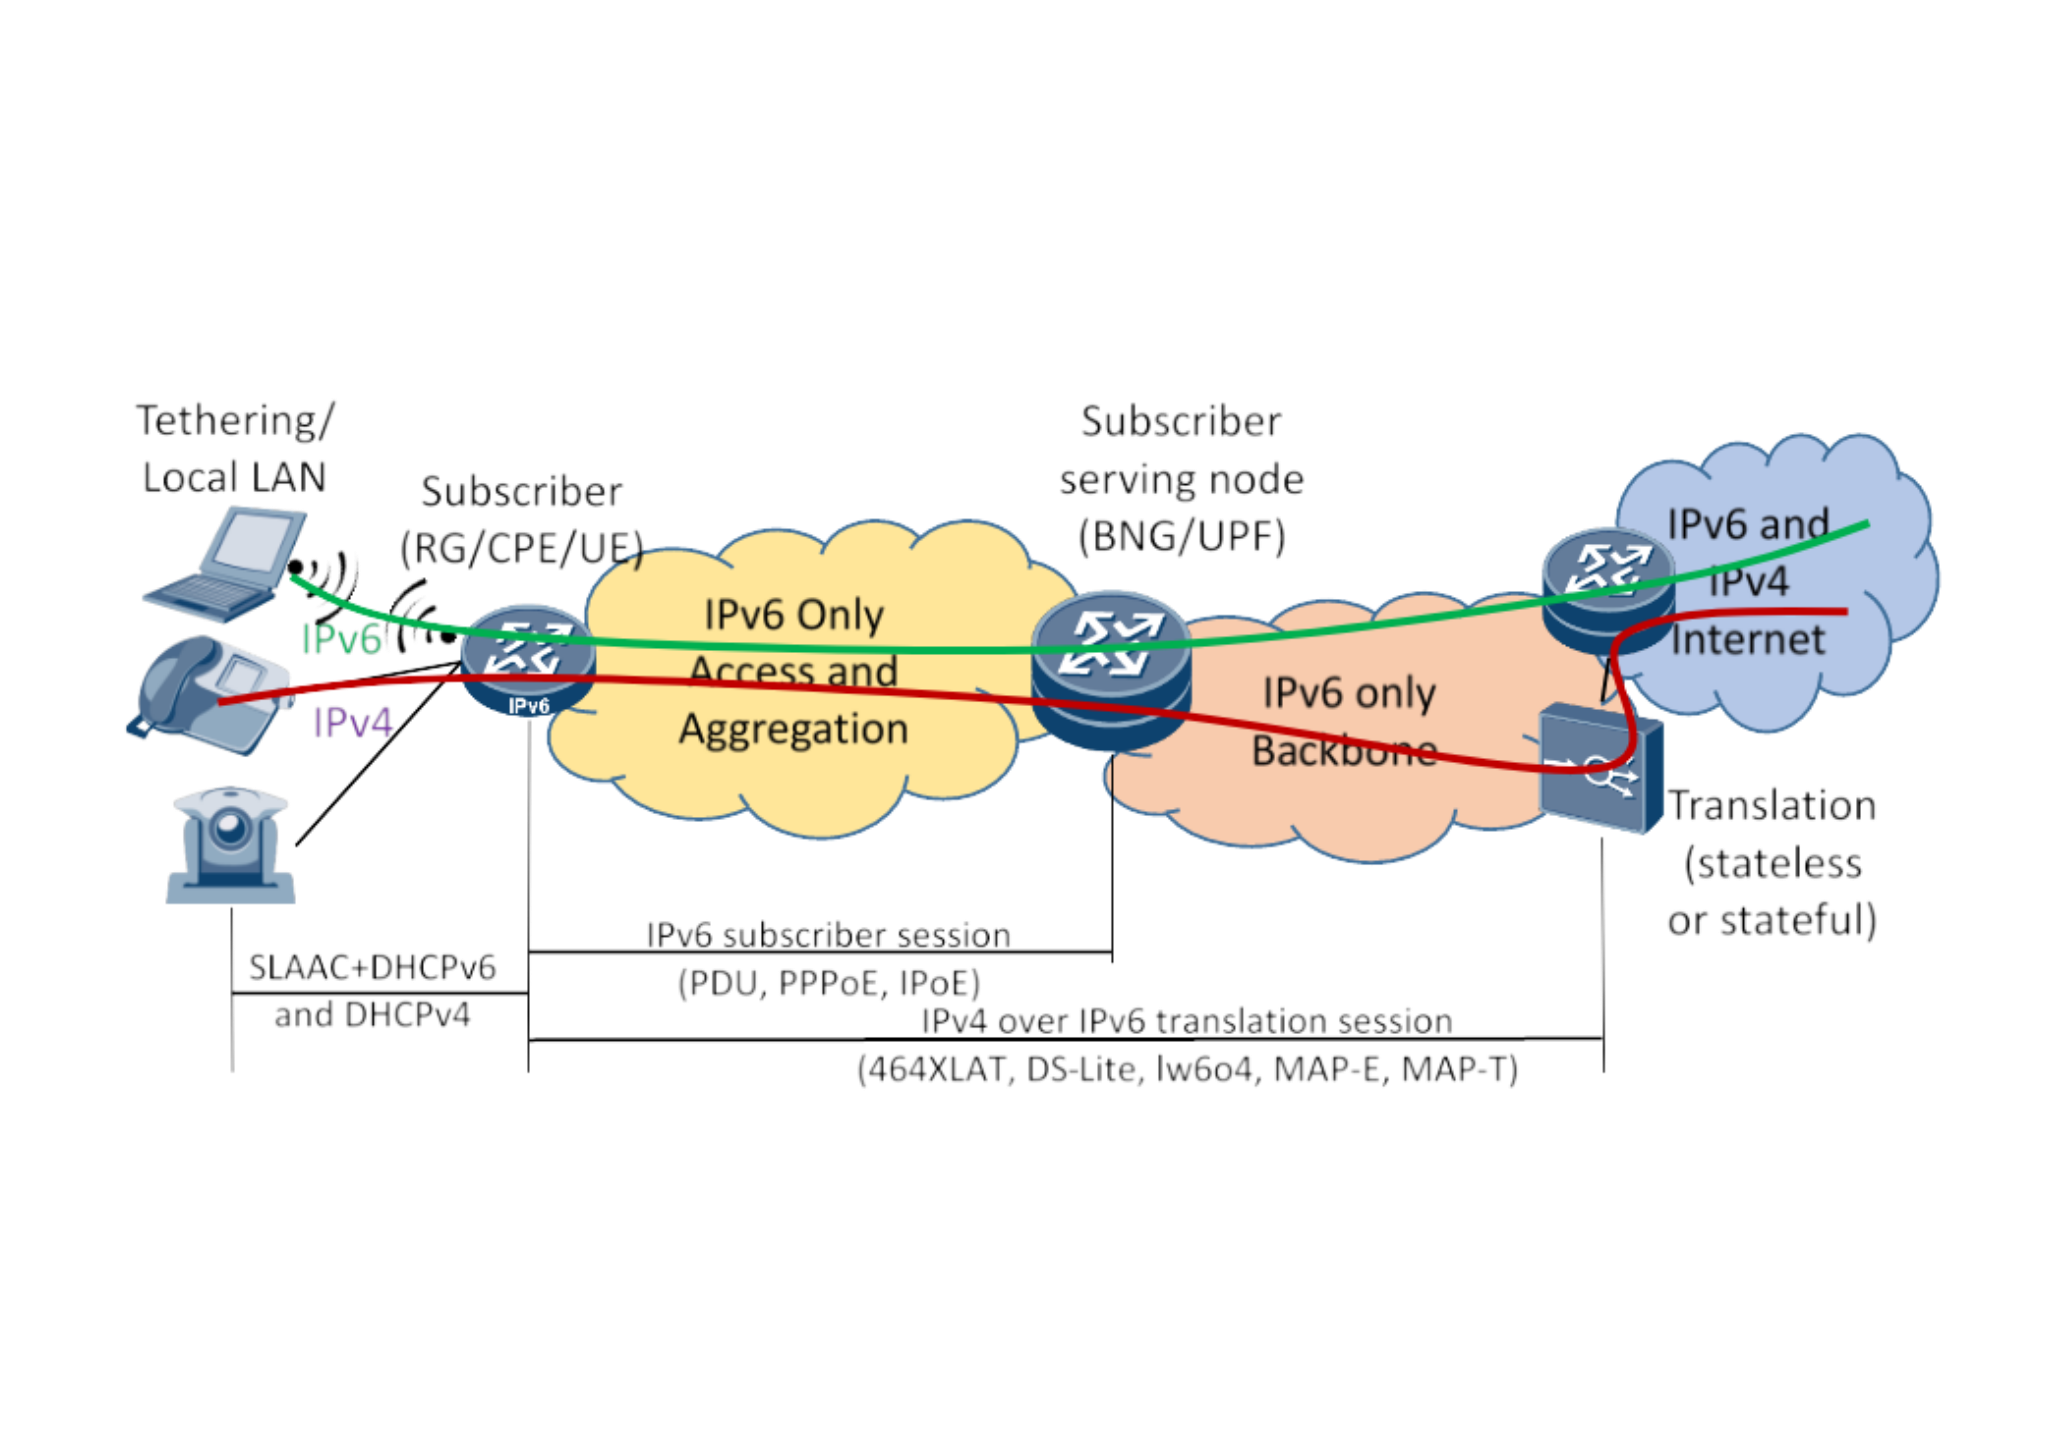
\includegraphics[keepaspectratio,alt={User devices connected to Internet via IPv6 infrastructure}]{vasilenko-IPv4aaS.png}}
\caption{User devices connected to Internet via IPv6 infrastructure}
\end{figure}

\begin{itemize}
\item
  464XLAT is the widely preferred translation technology now because it
  has a natural synergy with NAT64 (which is highly desirable by itself)
  and because it is the only solution supported on mobile devices. The
  centralized NAT64 engine is called PLAT, and is the same
  {[}\href{https://www.rfc-editor.org/info/rfc6146}{RFC6146}{]} as for
  ordinary NAT64. The client side is called CLAT, and is typically a
  stateless NAT46 translation
  {[}\href{https://www.rfc-editor.org/info/rfc7915}{RFC7915}{]}. A good
  analysis of deployment considerations is in
  \href{https://www.rfc-editor.org/info/rfc8683}{RFC 8683}, from which
  an operator might conclude \emph{not} to implement DNS64, since IPv4
  clients can simply use the normal DNS A records and the IPv4 service
  as if it was native.
\item
  DS-Lite was the most popular technology for a considerable period of
  time.
\item
  Lw6o4 has not gained significant market adoption.
\item
  Technically, MAP-E and MAP-T are stateless with significant related
  advantages: no need for logs, possible to implement on routers. But
  MAP needs a rather big IPv4 address space to be reserved for all
  clients (even when disconnected) and MAP is not available by default
  on the majority of Mobile OSes. As a result, MAP has a small market
  share.
\end{itemize}

\subsubsection{IPv4 as a service for mobile
devices}\label{ipv4-as-a-service-for-mobile-devices}

The diagram above covers IPv4aaS for a network. A special case is
IPv4aaS for a mobile device, especially when the device has only been
provided with a single /64 prefix, as is the case in most 3GPP
deployments. In this case, 464XLAT is the only available solution, and
as described in Section 6.3 of
\href{https://www.rfc-editor.org/info/rfc6877}{RFC 6877}, the CLAT will
use a specific address from that /64 prefix.

\subsubsection{Further details of NPTv6}\label{further-details-of-nptv6}

Network Prefix Translation (NPTv6)
{[}\href{https://www.rfc-editor.org/info/rfc6296}{RFC6296}{]} is a
special technology available only in IPv6. It exchanges prefixes between
``inside'' (private network) and ``outside'' (public network) of the
translation engine and modifies the IID. The IID is changed so as
preserve the transport layer checksum despite the prefix change. Hence,
it is transparent for all transport layer protocols. In principle it
would, for example, allow a site using ULA addresses
{[}\hyperref[addresses]{2. Addresses}{]} to communicate with global IPv6
addresses, but with some of the disadvantages of classical IPv4 NAT,
sometimes referred to as 1:1 NAT, and not to be confused with
masquerading address translation. The principal difference between NPTv6
and classical NAT is that it permits connection initiation in both
directions. However, it is not fully transparent for applications that
embed IP addresses at high layers (so-called ``referrals''). Hence, it
cannot be considered end-to-end transparent.

A particular difficulty is that SIP (Session Initiation Protocol for IP
telephony) will not work behind NPTv6 without the support of a proxy
mechanism {[}\href{https://www.rfc-editor.org/info/rfc6314}{RFC6314}{]}.

As stated above, NPTv6 is outlined in
\href{https://www.rfc-editor.org/info/rfc6296}{RFC 6296}; however,
although there is significant commercial support, it should be noted
that the RFC is experimental as of the time of this writing, so it is
not considered standards track.

It goes without saying that NPTv6 is \emph{never} justified by a
shortage of IPv6 addresses. Nevertheless, while there is controversy
about breaking end-to-end address transparency in IPv6, there are valid
use cases for such architectures, and breaking the end-to-end model is
more of an unfortunate side effect than a feature of such tools. Some
details on the "breakage" caused by NPTv6, and a comparison with
classical NAT, are given in
\href{https://www.rfc-editor.org/rfc/rfc6296.html\#section-5}{Section 5
of RFC 6296}.

In large scale deployments of wide area architectures, NPTv6 does enable
some compelling use cases which enable diversity in security platforms
such as stateful unified threat management devices (UTMs). These are
positioned in geographically and topologically diverse locations, but
require flexibility of \emph{external} layer 3 addressing to support
flow identification. Using NPTv6 to perform re-mapping of addressing
allows inspection engines to maintain the flow symmetry that is required
for stateful deep packet inspection engines to operate, as asymmetry
will cause them to mark all flows as incomplete. It is in this model
that it can be GUA to GUA, and this is a valid, supportable, and
definitely production deployed architecture.

In smaller deployments, NPTv6 can be leveraged to create stable
addressing inside a network that may be too small for PI address space,
but too large to operate without service provider diversity. In this
model, such as an SD-WAN deployment, a GUA or ULA prefix may be
deployed, delegated by a home office, other IT governance body, or a
local administrator, and mapped to one or more PA prefixes provided by
lower cost commercial internet services. This allows for internal
addressing to be stable, while providing a more robust connectivity
model, and the ability to more quickly switch providers if required by
leveraging dynamic addressing externally mapped to stable addressing
internally. This model more closely aligns with the current IPv4
architectures pervasively deployed nearly everywhere with stable
internal IPv4 addressing masqueraded to one or more PA addresses
provided by an upstream ISP.

\subsubsection{Further details on NAT66}\label{further-details-on-nat66}

NAT66 is currently a non-standards based mechanism for statefully
translating one or more IPv6 addresses to one or more other IPv6
addresses. When port translation is also provided (as is very common for
IPv4 NAT), the term NAPT66 may also be used.

It goes without saying that NAT66 is \emph{never} justified by a general
shortage of IPv6 addresses. Like NPTv6, NAT66 should be used only when
necessary or required. Moreover, is is also very important to understand
that the intent of these tools is to translate, hence the names. They
may play a part in compliance requirements, but they are - at their core
- translation tools and not security mechanisms. Address translation is
often deployed alongside stateful packet filtering, but the two are, in
actuality, exclusive toolkits. That is to say, they are not tied to each
other, and should be considered distinct - address translation is not a
security tool.

\subsubsection{\texorpdfstring{\hyperref[tunnels]{Previous}
\hyperref[obsolete-techniques]{Next}
\hyperref[coexistence-with-legacy-ipv4]{Top}}{Previous Next Top}}\label{previous-next-top-20}

\pagebreak

\subsection{Obsolete techniques}\label{obsolete-techniques}

As IPv6 has matured and people have gained operational experience,
various co-existence and transition techniques have either been shown to
be unsatisfactory or have simply been overtaken by events. This section
simply lists such techniques, with minimal explanation. Readers are
advised to ignore these techniques for new deployments, and to consider
removing them from existing deployments.

Tunneling IPv6 over IPv4, or the converse, remains fundamental to
co-existence, although various specific tunnel mechanisms are listed
below as obsolete.

Note that three such mechanisms (6to4, Teredo and ISATAP) have left
behind them some operational security risks related to IPv4 protocol
type 41, as described in
\href{https://doi.org/10.1007/978-3-030-72582-2_23}{Plight at the End of
the Tunnel - Legacy IPv6 Transition Mechanisms in the Wild}, preprint
\href{https://dataplane.org/jtk/publications/kgkp-pam-21.pdf}{here}.

\begin{itemize}
\item
  Transmission of IPv6 over IPv4 Domains without Explicit Tunnels
  {[}\href{https://www.rfc-editor.org/info/rfc2529}{RFC2529}{]}. As far
  as is known, this was never deployed in practice.
\item
  IPv6 Tunnel Broker
  {[}\href{https://www.rfc-editor.org/info/rfc3053}{RFC3053}{]}.
\item
  Connection of IPv6 Domains via IPv4 Clouds ("6to4")
  {[}\href{https://www.rfc-editor.org/info/rfc3056}{RFC3056}{]}
  {[}\href{https://www.rfc-editor.org/info/rfc3068}{RFC3068}{]}. The
  problems with this are documented in
  \href{https://www.rfc-editor.org/info/rfc6343}{RFC 6343} and it was
  largely deprecated by
  \href{https://www.rfc-editor.org/info/rfc7526}{RFC 7526}.
\item
  Teredo: Tunneling IPv6 over UDP through Network Address Translations
  (NATs) {[}\href{https://www.rfc-editor.org/info/rfc4380}{RFC4380}{]}.
\item
  SOCKS-based IPv6/IPv4 Gateway
  {[}\href{https://www.rfc-editor.org/info/rfc3089}{RFC3089}{]}.
\item
  ISATAP {[}\href{https://www.rfc-editor.org/info/rfc5214}{RFC5214}{]}.
\item
  6rd {[}\href{https://www.rfc-editor.org/info/rfc5569}{RFC5569}{]}.
\item
  An Incremental Carrier-Grade NAT (CGN) for IPv6 Transition
  {[}\href{https://www.rfc-editor.org/info/rfc6264}{RFC6264}{]}.
\item
  6a44 {[}\href{https://www.rfc-editor.org/info/rfc6751}{RFC6751}{]}.
\item
  In the context of NAT64,
  \href{https://www.rfc-editor.org/info/rfc7050}{RFC 7050} should no
  longer be used.
\end{itemize}

\subsubsection{\texorpdfstring{\hyperref[translation-and-ipv4-as-a-service]{Previous}
\hyperref[ipv6-primary-differences-from-ipv4]{Next}
\hyperref[coexistence-with-legacy-ipv4]{Top}}{Previous Next Top}}\label{previous-next-top-21}

\pagebreak

\subsection{IPv6 primary differences from
IPv4}\label{ipv6-primary-differences-from-ipv4}

This book intentionally describes IPv6 as the "new normal" IP protocol,
but this section mentions the main ways that it differs from IPv4, using
terminology from \hyperref[ipv6-basic-technology]{2. IPv6 Basic
Technology}.

IPv6 is very similar for transit routing, but has some considerable
differences on the first hop for hosts as well as for routers that do
more than pure routing.

The primary differences are:

\begin{itemize}
\item
  The first difference is desirable and expected: IPv6 has a four times
  bigger address size (128 bits against 32 bits).

  SLAAC is more used on IPv6 than DHCPv6. A SLAAC subnet prefix is 64
  bits for historical reasons that are fixed in many standards. 2\^{}64
  hosts are of course not possible in one subnet, but the address space
  is reserved even for a smartphone. Hence, it is disputable what is the
  effective IPv6 address space. It is bigger than 2\^{}64 bits but the
  64 IID bits are utilized for privacy and security, not for addressing
  \emph{per se}.
\item
  NAT44 is a common solution in IPv4 networking.

  NAT66 is discouraged by IETF and not specified as a standard. IPv6
  end-to-end connectivity is considered a big value.
\item
  IPv4 has only one address per interface (without special hacks).

  Many IPv6 addresses on every interface are the norm. It is not just
  different address types (LLA, ULA, and GUA) but additionally many
  instances of GUA and ULA for security or virtualization reasons. The
  popular ChromOS has seven IPv6 addresses as the minimum. Additionally,
  the number of IPv6 addresses per interface could almost double in the
  case of link renumbering.
\item
  IPv4 has only centralized DHCPv4 address acquisition.

  IPv6 has additionally distributed address acquisition by SLAAC which
  is widely adopted. SLAAC considerably changes the logic of the link
  operation. (The problems caused by broadcast IPv4 ARP are replaced by
  the problems caused by multicast IPv6 Neighbor Solicitation!)
\item
  IPv4 has a complex (many fields) and theoretically variable header
  that is practically fixed because options are not widely used.

  IPv6 has a simple and fixed header. Additionally, IPv6 could have
  extension headers that permit unlimited protocol extensibility at the
  data plane. Many extension headers are already used in limited
  domains. Just like IPv4 options, deployment of new IPv6 extensions
  headers and options across the open Internet is problematic.
\item
  IPv4 fragmentation is in the basic header and permitted in transit.

  IPv6 fragmentation uses an extension header and is prohibited in
  transit.
\item
  IPv4 address resolution on the link by ARP protocol is at layer 2 (for
  the IEEE 802 media it is an IEEE 802 frame). IPv6 address resolution
  on the link by ND protocol is at layer 3 (IPv6 packet over LLA or
  other IP addresses).
\item
  Multicast is not needed for IPv4 itself.

  Multicast is mandatory for the IPv6 link operation. Many ND functions
  are using multicast. That may create advantages (for Ethernet) and
  disadvantages (for many types of wireless).
\end{itemize}

The list above is not comprehensive, but the other differences are
probably smaller.

An obvious question is: With all these differences, what is the
difference in performance between IPv6 and IPv4? There is no simple
answer to this question. Since the IPv6 packet header is 20 bytes larger
than for IPv4, the raw payload throughput of a link carrying full sized
IPv6 packets is slightly less than for IPv4 (about 1.3\% less for 1500
byte packets). However, many other factors come into play and
measurements often show better end-to-end performance for IPv6. For
example, in most countries
\href{https://www.google.com/intl/en/ipv6/statistics.html\#tab=per-country-ipv6-adoption}{Google
statistics} show lower latency (transit time) for IPv6. The safest
summary is that there is no significant performance difference.

\subsubsection{\texorpdfstring{\hyperref[obsolete-techniques]{Previous}
\hyperref[security]{Next}
\hyperref[coexistence-with-legacy-ipv4]{Top}}{Previous Next Top}}\label{previous-next-top-22}

\pagebreak

\section{Security}\label{security}

Security has ever-growing importance in general and the IP protocol has
been a big area for security research and development. The majority of
IPv4 practices remain applicable to IPv6. Exceptions exist for aspects
of the first hop and for extension headers that are significantly
different in IPv6. Distributed address acquisition (SLAAC,
\hyperref[auto-configuration]{2. Auto-configuration}) creates its own
additional security challenges. Multiple addresses per host improve
privacy, but not without complications. Extension headers give IPv6
great flexibility and extensibility that may be abused, leading to
additional security precautions.

Initially, it was expected that end-to-end cryptography (encryption and
authentication) would be a mandatory part of IPv6 (IPsec,
\href{https://www.rfc-editor.org/info/rfc4301}{RFC 4301} and SEND,
\href{https://www.rfc-editor.org/info/rfc3971}{RFC 3971}). This proved
unrealistic, so cryptography has been accepted as optional at the
networking layer, exactly as it is for IPv4. At the same time,
cryptography has become widespread at the transport or application
layers.

IPv6 aims at restoring end-to-end connectivity to the networking layer.
Therefore, IPv6 security in no way relies on the presence of network
address translation. IPv6 has no standardized NAT66 and even network
prefix translation (NPTv6,
\href{https://www.rfc-editor.org/info/rfc6296}{RFC 6296}) is little
used. NAT or NPTv6 provide at best weak security protection at the
network boundary, so this is not seen as a defect. The normal approach
to boundary security for IPv6 is a firewall; most firewall products
support IPv6 as well as IPv4. Topology hiding is addressed in a later
section of this chapter.

Today, the ``Zero-trust'' approach in security tends to move the stress
from perimeter protection to the authentication and encryption for all
traffic (including internal for any perimeter). If this approach
succeeds, some enterprises may choose to reduce the role of firewalls in
future. IPv6 is well positioned for this change.

A good design and policy rule to follow is that in a dual-stacked
deployment, which is by and large the largest percentage of IPv6
deployments, security policy for IPv4 and IPv6 should match in order to
ensure consistency of operational and user experience. In an IPv6-only
deployment, implementation of policy should be derived from overall
network security policy, taking into account protocol specifications
that may require adjustments from legacy IP (i.e. differences in ICMP
handling between IPv4 and IPv6).

There is a good overview of IPv6 security in
\href{https://www.rfc-editor.org/info/rfc9099}{RFC 9099}. This is a good
repository of references to many documents on various IPv6 security
aspects.

\hyperref[layer-2-considerations]{Layer 2 considerations}

\hyperref[filtering]{Filtering}

\hyperref[topology-obfuscation]{Topology obfuscation}

\subsubsection{\texorpdfstring{\hyperref[list-of-contents]{Back to main
Contents}}{Back to main Contents}}\label{back-to-main-contents-3}

\pagebreak

\subsection{Layer 2 considerations}\label{layer-2-considerations}

IPv6 is comparatively flexible at the link layer. Flexibility typically
comes with complexity, which can drive security challenges.

Initially, there was a belief that cryptographic SEcure Neighbor
Discovery (SEND, \href{https://www.rfc-editor.org/info/rfc3971}{RFC
3971}) would resolve the majority of neighbor discovery risks.
Unfortunately, SEND was not accepted by the market. Hence, the security
problems discussed in \href{https://www.rfc-editor.org/info/rfc3756}{RFC
3756} section 4.1 are still active:

\begin{itemize}
\tightlist
\item
  A malicious node could answer to Duplicate Address Discovery (DAD) for
  any request of a legitimate node, amounting to a denial of service
  attack;
\item
  A malicious node could poison the neighbor cache of another node
  (especially the router) to intercept traffic directed to another node
  (man-in-the-middle attack); it is possible for neighbor solicitation
  and neighbor advertisement in many different cases.
\end{itemize}

There is no big difference here from IPv4 ARP spoofing. Of course, the
danger only exists if a bad actor succeeds in implanting a malicious
node. Where this is felt to be a significant risk, the strongest
protection method is host isolation on a separate link with a separate
dedicated /64 prefix. IPv6 has enough address space to follow this
strategy. All subscribers (including mobile) already have at least one
/64 prefix. A /56 prefix is considered as the minimum for ordinary
domestic subscribers with the possibility for /48 for even a small
business. The latter would theoretically allow 65,535 hosts each to have
their own /64.

An alternative method of protection is Source Address Validation
Improvement (SAVI) - see
\href{https://www.rfc-editor.org/info/rfc6620}{RFC 6620} which is based
on the full Neighbor Discovery (ND) exchange monitoring by the switch to
dynamically install filters. Like SEND, it is not a very popular
solution.

Cellular mobile links (3GPP etc.) are always a point-to-point tunnel.
Hence, it was possible to greatly simplify the ND protocol (address
resolution and DAD are unnecessary) to avoid complexity and the majority
of security threats -- see
\href{https://www.rfc-editor.org/info/rfc7849}{RFC 7849}.

It is of the same importance as for IPv4 to restrict who could claim the
default router and DHCP server functionality because it is the best way
to organize man-in-the-middle attacks. Hence, RA-Guard
\href{https://www.rfc-editor.org/info/rfc6105}{RFC 6105} and
DHCPv6-Shield \href{https://www.rfc-editor.org/info/rfc7610}{RFC 7610}
are defined. Unfortunately, there is a possibility to hide the purpose
of a packet by prepending the transport layer with extension headers
(especially dangerous fragmentation). Hence,
\href{https://www.rfc-editor.org/info/rfc7113}{RFC 7113} and
\href{https://www.rfc-editor.org/info/rfc7112}{RFC 7112} are
additionally needed for protection against rogue Router or DHCP.

There is a new security attack vector related to IPv6 specifically.
SLAAC address acquisition is distributed, so the router may not know all
addresses configured on the link even if all ND exchange is monitored by
the router. Hence, the router needs to request address resolution after
the first packet of a new session is received from an external source.
At the same time, the IPv6 link address space is huge (2\^{}64) by
default. Hence, it is potentially possible to force the router to
perform address resolution a huge number of times (even from an external
network). It is an effective DoS attack that has simple protection
measures. \href{https://www.rfc-editor.org/info/rfc6583}{RFC 6583}
discusses how to rate-limit the number of address resolution requests or
minimize subnet size.

ND heavily relies on multicast which may create problems in the wireless
environment. See \hyperref[address-resolution]{2. Address resolution}
and
\href{https://datatracker.ietf.org/doc/draft-vyncke-6man-mcast-not-efficient}{Multicast
efficiency}. ND DoS activity may be effective for that reason but the
attacker should be local to the link. Hence, perimeter security may
help. The multicast storm is less of a problem in a wired environment
because of MLD snooping typically implemented on the link
(\href{https://www.rfc-editor.org/info/rfc4541}{RFC 4541}).

IPv6 has a new feature that improves privacy. It is normal for an IPv6
host to have many IP addresses for the same interface, often with
unpredictable (pseudo-random) IID values. Some IP addresses may be used
temporarily (\href{https://www.rfc-editor.org/info/rfc8981}{RFC 8981})
which creates a challenge for intermediate Internet nodes to trace
suspicious user activity, for the same reason that it protects privacy.

\subsubsection{\texorpdfstring{\hyperref[filtering]{Next}
\hyperref[security]{Top}}{Next Top}}\label{next-top-3}

\pagebreak

\subsection{Filtering}\label{filtering}

Filtering is a big part of safe Internet connection. IPv6 filtering in
general may be easy because of the hierarchical address plan. However,
each filter almost always consumes four times more resources in
products. This may affect scalability or performance, if equipment is
underprovisioned.

The majority of practices do not change with IPv6 adoption:

\begin{itemize}
\tightlist
\item
  \href{https://www.rfc-editor.org/info/bcp38}{BCP 38} recommends
  carriers to filter traffic based on \emph{source} addresses on ingress
  from the client to prevent address spoofing. Source addresses in the
  range delegated to this client are allowed; other sources addresses
  should be filtered (except for the case mentioned in
  {[}\hyperref[multi-prefix-operation]{6. Multi-prefix operation}{]}).
  Operators that do not implement BCP38 are condoning address spoofing.
\item
  "Martian" addresses should be filtered on the perimeter according to
  \href{https://www.rfc-editor.org/info/rfc6890}{RFC 6890}. In the case
  of IPv6, this refers to the
  \href{https://www.iana.org/assignments/iana-ipv6-special-registry/iana-ipv6-special-registry.xhtml}{IANA
  IPv6 Special-Purpose Address Registry}.
\item
  Filtering on \href{https://www.rfc-editor.org/info/rfc7454}{BGP
  Peering} and \href{https://www.rfc-editor.org/info/rfc8210}{RPKI} do
  not change for IPv6.
\item
  The router's control plane protection
  {[}\href{https://www.rfc-editor.org/info/rfc6192}{RFC6192}{]} is
  universal for IPv6 or IPv4.
\item
  \href{https://www.rfc-editor.org/info/rfc5635}{Remote Triggered Black
  Hole} is the same for IPv4 and IPv6, except that the prefix for IPv6
  \href{https://www.rfc-editor.org/info/rfc6666}{100::/64} has been
  defined separately.
\item
  All IGP protocols should filter announcements for the local link
  according to \href{https://www.rfc-editor.org/info/rfc5082}{RFC 5082}.
  In the case of IPv6, this means that announcements are allowed only
  from link-local addresses.
\item
  \href{https://www.rfc-editor.org/info/rfc4641}{DNSSEC} is recommended,
  independent of A or AAAA requests.
\end{itemize}

Some filters are specific to IPv6.

The biggest difference is related to the typical prefix size (/64).
Filtering anything longer than this is useless, because of the
unpredictable temporary addresses that a host may generate. Moreover, if
there is a desire to filter one subscriber it may be apprpriate to
filter even shorter prefixes, such as a /56. It is recommended to filter
/64 initially and then monitor the situation; if the problem persists,
then filter /60, then /56. /48 is the maximum that may belong to an
ordinary subscriber, so it does not make sense to filter shorter
prefixes than that to block a single subscriber.

The address plan design of an organization may be different, including
/128 addresses with DHCPv6 configuration, but it is never possible to
know this from the outside. If the organization employs SLAAC then again
/64 is the minimum that makes sense to filter.

The addresses of different scopes should be filtered at respective
borders:

\begin{itemize}
\tightlist
\item
  LLA should be not forwarded outside of the link according to
  \href{https://www.rfc-editor.org/info/rfc4291}{IPv6 Addressing
  Architecture},
\item
  ULA should be filtered at organization borders according to
  \href{https://www.rfc-editor.org/info/rfc4193}{RFC 4193},
\item
  Multicast addresses have 5 defined scopes (Interface, Link, Admin,
  Site, and Organization) according to
  \href{https://www.rfc-editor.org/info/rfc4291}{IPv6 Addressing
  Architecture} that should be filtered at respective borders. For the
  lowest scopes, the perimeter is evident and typically hard-coded into
  nodes. For the scopes with flexible borders (like Admin, Site,
  Organization) it needs a special configuration.
\end{itemize}

PMTUD operation is more important in IPv6 because fragmentation is
prohibited in transit. Hence, ICMP filtering may do more harm in IPv6.
It is discussed in
\href{https://www.rfc-editor.org/info/rfc4890}{Recommendations for
ICMPv6 filtering} what should be dropped or permitted.

Security devices and destination nodes should check that the first
fragment should have all headers (including the transport layer) and
fragments should not have an overlap according to
\href{https://www.rfc-editor.org/info/rfc8200}{RFC 8200}.

\href{https://www.rfc-editor.org/info/rfc9288}{Filtering recommendations
for packets with extension headers} is oriented for the transit case
where excessive filtering is common. This RFC motivates what particular
EHs to permit, drop, reject (with ICMP), rate-limit, or ignore. It is
important to mention that these additional actions are recommended in
addition to the basic rule of
\href{https://www.rfc-editor.org/info/rfc7045}{RFC 7045} to allow by
default the transmission of all extension headers in transit.

Limiting ND messages on the link is discussed in
\hyperref[address-resolution]{Address resolution}.

There is a risk for IPv4-only networks caused by IPv6 preference
programmed into hosts. The activation of IPv6 by a malicious node could
create security problems.
\href{https://www.rfc-editor.org/info/rfc7123}{Security Implications of
IPv6 on IPv4 Networks} discusses what is important to block in this
scenario. These are primarily different tunneling protocols that might
help to bypass perimeter security, and rogue DHCP or Router code for a
man-in-the-middle attack.

\subsubsection{\texorpdfstring{\hyperref[layer-2-considerations]{Previous}
\hyperref[topology-obfuscation]{Next}
\hyperref[security]{Top}}{Previous Next Top}}\label{previous-next-top-23}

\pagebreak

\subsection{Topology obfuscation}\label{topology-obfuscation}

There are various operational contexts in which an operator needs to
obfuscate or otherwise hide a network\textquotesingle s topology,
equipment, and hosts from outsiders. Since IPv6 promotes end-to-end
addressing, the question arises of how to achieve topology hiding or
obfuscation in the absence of network address translation (NAT).

One important context for this is networks that must conform to
standards such as Payment Card Industry Data Security Standard
Requirements (PCI-DSS), issued by the
\href{https://www.pcisecuritystandards.org}{PCI Security Standards
Council}. (This standard can be
\href{https://docs-prv.pcisecuritystandards.org/PCI\%20DSS/Standard/PCI-DSS-v4_0.pdf}{downloaded}
free of charge, but beware that you must agree to a license in order to
do so.) PCI-DSS requires an enterprise that stores certain types of
customer data to do so on servers that are effectively isolated from the
Internet and undiscoverable from outside the enterprise. Yet these
systems might also be offering Web services to clients anywhere in the
Internet. A common solution to this dilemma for IPv4 has two parts:

\begin{enumerate}
\def\labelenumi{\arabic{enumi}.}
\item
  A "demilitarized zone" (DMZ) between the Internet and the core of the
  enterprise network.
\item
  When a server in the core communicates with a client elsewhere in the
  Internet, the requirement to hide the server is commonly satisfied by
  IPv4 NAT between the server and the DMZ.
\end{enumerate}

It goes without saying that such traffic will flow through a firewall
(which PCI-DSS refers to as a Network Security Device or NSD). The
question is how should such a system obscure the
server\textquotesingle s regular IPv6 address as effectively as NAT
obscures its IPv4 address. Note that PCI-DSS (version 4, March 2022)
does not require NAT, although it is mentioned as a solution for IPv4.
For IPv6, it suggests using temporary addresses
{[}\href{https://www.rfc-editor.org/info/rfc8981}{RFC8981}{]} for
outgoing sessions (although it cites an obsoleted RFC). Placing system
components behind proxy servers is also suggested, and it seems probable
that large installations will do this anyway to support load balancing
{[}\href{https://www.rfc-editor.org/info/rfc7098}{RFC7098}{]}. Proxy
servers and load balancers will intrinsically hide the core topology
from attackers.

Other aspects of topology hiding were discussed in
\href{https://www.rfc-editor.org/info/rfc4864}{RFC 4864}, but that
document is significantly out of date.

Another common architectural scenario entails dis-aggregating a GUA
allocation, typically an RIR provided address block, and announcing only
the part of the assignment requiring public access, leaving the prefix
requiring obfuscation unannounced within the global DFZ (default free
zone). This model allows for a similar level of topology obscurement
without the added configuration complexity and potentially inconsistent
behavior of ULA or address translation. It should be noted, however,
that while this design model does reduce complexity at the host and
network layer, it may add minor routing complexity at the border and
incur risk of unintentionally leaking the GUA prefix that has been
earmarked for local-only use. In the latter case, use of a "belt and
suspenders" implementation of creating route policy in addition to
access control lists preventing prefix use is frequently employed.

\subsubsection{\texorpdfstring{\hyperref[filtering]{Previous}
\hyperref[network-design]{Next}
\hyperref[security]{Top}}{Previous Next Top}}\label{previous-next-top-24}

\pagebreak

\section{Network Design}\label{network-design}

A first very general remark is that since IPv6 is a datagram protocol,
whose routing relies on longest matching of address prefixes, the
highest level of design decisions are identical to those for IPv4.

There is one constraint that does not apply to IPv6: there is
effectively no theoretical limit to the number of hosts per subnet.
(Mathematically, there is a limit of about 18.10\^{}18 nodes on a /64
subnet, but this is of no practical concern.) However, most network
designers will never place hundreds or thousands of hosts on a single
subnet, for performance reasons.

A network designer does, however, have more flexibility with IPv6. If an
enterprise has a /48 prefix, 16 bits are available to identify more than
65 thousand individual subnets, a luxury for most IPv4 network
designers. But we can go even further: there are deployment models where
handing out a complete /64 prefix to a single node may be beneficial
(e.g., if that node may contain a large number of virtual machines).
Large enterprises, and of course carriers, can simply obtain more
address space (i.e., a prefix shorter than /48) if they need it. In
practice, address space should \emph{never} be a limiting factor for
IPv6 network design.

Setting these aspects aside, there is no reason why an IPv6 network will
have a different macroscopic design than an IPv4 network. The detailed
approach will vary.

\begin{itemize}
\item
  If the intention is a "retrofit" where IPv6 support is added to an
  existing IPv4 network, major topology will not change, but items such
  as border routers, firewalls, interior routers, and DMZs will need to
  be upgraded accordingly. Clearly, a specific choice of IPv6/IPv4
  coexistence mechanism must be made, and applied consistently. In the
  past, most networks have chosen the original dual-stack approach
  {[}\hyperref[dual-stack-scenarios]{3. Dual stack scenarios}{]} but
  designers should now also consider
  \hyperref[translation-and-ipv4-as-a-service]{3. Translation and IPv4
  as a service}. A priority will be adding comprehensive IPv6 support to
  the NOC and all its systems, before deployment to users. An equal
  priority will be training of all NOC and support personnel: they need
  to be IPv6 evangelists.
\item
  If the intention is a "greenfield" deployment with no existing IPv4
  network, the main topology will be conventional, but a specific choice
  of mechanism for IPv4 as a service must be made
  {[}\hyperref[translation-and-ipv4-as-a-service]{3. Translation and
  IPv4 as a service}{]}. The NOC must be designed from the start based
  on IPv6, with the ability to manage IPv4 as a service.
\item
  A specific difference between a retrofit design and a greenfield
  design is that an existing IPv4 network almost inevitably has subnets
  limited to 256 or fewer hosts, often as few as 64. Since the normal
  subnet prefix in IPv6 is a /64, there is no such limitation in a
  greenfield deployment of IPv6. However, for practical reasons such as
  the rate of link-local multicasts, very large subnets should be
  avoided. As noted elswehere {[}\hyperref[address-resolution]{2.
  Address resolution}{]} this applies particularly to wireless networks.
\end{itemize}

This chapter continues with a discussion of address planning, inevitably
combined with subnet design.

\hyperref[address-planning]{Address Planning}

\hyperref[prefix-per-host]{Prefix per Host}

\subsubsection{\texorpdfstring{\hyperref[list-of-contents]{Back to main
Contents}}{Back to main Contents}}\label{back-to-main-contents-4}

\pagebreak

\subsection{Address Planning}\label{address-planning}

As you would expect, in IPv6 networks all nodes may have globally unique
addresses. All networks will be given at least a /64 global prefix to
operate. Carriers should deliver a shorter prefix to their subscribers
(typically in the range /48 through /56)
{[}\href{https://www.rfc-editor.org/info/rfc6177}{RFC6177}{]}, which
allows multiple /64 subnets within subscriber organizations or home
environments. Even a home customer can have a public network prefix to
be split into smaller networks, which is a paradigm shift from ``hiding
behind NAT'' on a few public IPv4 addresses (or even inside
\texttt{100.64.0.0/10}
{[}\href{https://www.rfc-editor.org/info/rfc6598}{RFC6598}{]}).

In IPv6 networks, it is often necessary to manage received prefixes,
even if it is done automatically by a CE router. Likewise, network
operators receive large address blocks from the RIRs and must plan their
address distribution in order to handle address blocks assigned to
customers or their own infrastructure.

For instance, we can start with a network operator. Consider a carrier
called ``ISP'' that received the prefix \texttt{2001:db8::/32}. It is
necessary to separate address blocks asigned for home customers,
corporate customers and for ISP\textquotesingle s own infrastructure.
First, let\textquotesingle s see what space is available for planning:

\begin{verbatim}
 Global ID -Subnets- -- Interface IDs --
| 32 bits | 32 bits |   64 bits         |
 2001:0db8:0000:0000:0000:0000:0000:0000
\end{verbatim}

The first 32 bits will remain unchanged, of course, and the last 64 bits
will always belong to the ending subnet nodes. It leaves us the 32 bits
between them to work with. Keep in mind that there is no concern about
exhaustion of IPv6 addresses(or prefixes), seeing that this single
assignment for an autonomous system (ISP) gives the equivalent of the
entire IPv4 Internet address space to work with. And this is not about
unique addresses, but /64 network prefixes! As an analogy, a /64 prefix
would be the equivalent of leasing a public IPv4 address to a single
network or subscriber. In this way, in IPv6 planning we can favor
organization and clearer management instead of saving as many addresses
as possible. On IPv6 networks it makes no sense to count unique
addresses; instead, we consider the number of available /64 prefixes.
Think of a /64 prefix as a standard unit that fits all network sizes.

Remember that our 32-bit subnet space embodies 4 billion /64 networks,
so there is room for good planning and management as there will be no
address shortage on any reasonable timescale. A good addressing plan
should always have room for future expansion and favor network
aggregation and management. (Of course, even IPv6 address space is not
infinite, but the policies applied by the various Regional Address
Registries will avoid any risk of exhaustion.) For this reason, in the
following example, we will use the technique known as \textbf{leftmost},
to guarantee a more balanced distribution on all available space. Back
to the example, consider our 32 bits where we can use the first 4 (one
"nibble" or hexadecimal character) to assign sixteen regions, as 0 to F,
resulting in a /36 per region. A region may be a data center,
geographical area or a branching network.

\begin{verbatim}
A. Region A - Main Datacenter
B. Region B - City south
C. Region C - City north
\end{verbatim}

So the first layer of our address plan may look like this:

\begin{verbatim}
2001:0db8:0000::/36 - Reserved
2001:0db8:1000::/36 - Reserved
2001:0db8:2000::/36 - Reserved
2001:0db8:3000::/36 - Reserved
2001:0db8:4000::/36 - Reserved
2001:0db8:5000::/36 - Reserved
2001:0db8:6000::/36 - Reserved
2001:0db8:7000::/36 - Reserved
2001:0db8:8000::/36 - Reserved
2001:0db8:9000::/36 - Reserved
2001:0db8:A000::/36 - Region A
2001:0db8:B000::/36 - Region B
2001:0db8:C000::/36 - Region C
2001:0db8:D000::/36 - Reserved
2001:0db8:E000::/36 - Reserved
2001:0db8:F000::/36 - Reserved
\end{verbatim}

(Note: We are using uppercase characters to distinguish the locally
assigned prefixes; this breaks the usual recommendation to use
lowercase.)

Each region has functional divisions that may earn one or more address
blocks. Each division could be for instance:

\begin{enumerate}
\def\labelenumi{\arabic{enumi}.}
\tightlist
\item
  Internal infrastructure
\item
  Domestic clients
\item
  Corporate clients Using the same logic you can split a
  region\textquotesingle s /36 into 16 /40 prefixes, so it is easier to
  manage. Keep in mind that it is possible to assign more prefixes for
  each one if necessary. Now let\textquotesingle s see the address plan
  for \textbf{Region A} where we have 16 /40 prefixes:
\end{enumerate}

\begin{verbatim}
2001:0db8:A000::/40 - Corporate clients ---|
2001:0db8:A100::/40 - Corporate clients    |---> 1024 x /48 prefixes
2001:0db8:A200::/40 - Corporate clients    |
2001:0db8:A300::/40 - Corporate clients ---|
2001:0db8:A400::/40 - Internal infrastructure ---> 256 x /48 prefixes for infrastructure
2001:0db8:A500::/40 - Reserved
2001:0db8:A600::/40 - Reserved ---> 768 x /48 prefixes for expansion
2001:0db8:A700::/40 - Reserved
2001:0db8:A800::/40 - Domestic clients ---|
2001:0db8:A900::/40 - Domestic clients    | 2048 x /48 prefixes
2001:0db8:AA00::/40 - Domestic clients    | or
2001:0db8:AB00::/40 - Domestic clients    | 2001:db8:A800::/37
2001:0db8:AC00::/40 - Domestic clients    | or 
2001:0db8:AD00::/40 - Domestic clients    | 2048 x 256 x /56 prefixes
2001:0db8:AE00::/40 - Domestic clients    |
2001:0db8:AF00::/40 - Domestic clients ---|
\end{verbatim}

As shown above, we have a good measure for corporate and home customers,
plus a room for expansion, added by a generous /40 just for internal
infrastructure. Of course, this can be changed according to needs on
each case. For example, increase the number of prefixes for corporate
clients, or take some space in infrastructure reserved part, which is
very large. Even add another entire /36 block for the same region. If
you do the math, the numbers are always very loose so that we can always
give preference to address organization, aggregation and good
management.

\subsubsection{Client delegations}\label{client-delegations}

It is recommended to delegate at least a /48 block to clients. Best
practice says that corporate clients always receive at least a /48
prefix and domestic clients receive at least a /56 prefix. Mobile access
clients may receive a single /64 (but more would be better, to allow
IPv6 "hot spots"). See below with 2 prefixes from Region
A\textquotesingle s /40 block: a /48 assigned to a corporate customer
and a /56 to a domestic customer:

\begin{enumerate}
\def\labelenumi{\arabic{enumi}.}
\tightlist
\item
  \texttt{2001:0db8:A3CC:0000::/48} The least four Zeros shows 16 bits
  given within a /48 prefix, available to address 2\^{}16=65536 /64
  subnets.
\item
  \texttt{2001:0db8:ABDD:DD00::/56} The least two Zeros represent 8 bits
  given within a /56 prefix available to address 2\^{}8=256 /64 subnets.
\end{enumerate}

See that a single corporate client is up to a virtually unlimited
address space and a domestic subscriber may have 256 subnets on a home
network. Once a client leases an address block it has to split it for
given subnets inside the network. Let\textquotesingle s take that same
home customer with the \texttt{2001:0db8:ABDD:DD00::/56} prefix and see
what we can do:

\begin{verbatim}
2001:0db8:ABDD:DD00::/64 ---> Main home subnet
2001:0db8:ABDD:DD01::/64 ---> Wifi subnet
2001:0db8:ABDD:DD02::/64 ---> Wifi Guest subnet
2001:0db8:ABDD:DD(...)::/64 ---> Reserved
2001:0db8:ABDD:DDFE::/64 ---> IoT subnet
2001:0db8:ABDD:DDFF::/64 ---> VoIP subnet
\end{verbatim}

ISP customers typically lease address blocks through \textbf{DHCPv6
prefix delegation}
{[}\href{https://www.rfc-editor.org/info/rfc8415}{RFC8415}{]}. Instead
of acquiring only one Internet facing address, the customer premises
router requests an entire GUA block. Once it has it, the smaller /64
blocks are typically handled as a prefix pool, where each is assigned to
a internal subnet.

\subsubsection{Other sources of
information}\label{other-sources-of-information}

Daryll Swer has written an excellent
\href{https://www.daryllswer.com/ipv6-architecture-and-subnetting-guide-for-network-engineers-and-operators/}{blog}
that covers subnet and addressing design (also available from
\href{https://blog.apnic.net/2023/04/04/ipv6-architecture-and-subnetting-guide-for-network-engineers-and-operators/}{APNIC}).

Although quite old, the following book may be helpful:
\href{https://www.oreilly.com/library/view/ipv6-address-planning/9781491908211/}{IPv6
Address Planning} by Tom Coffeen.

\subsubsection{\texorpdfstring{\hyperref[prefix-per-host]{Next}
\hyperref[network-design]{Top}}{Next Top}}\label{next-top-4}

\pagebreak

\subsection{Prefix per Host}\label{prefix-per-host}

IPv6 nodes very often have multiple valid addresses, for example by
configuring temporary addresses
{[}\href{https://www.rfc-editor.org/info/rfc8981}{RFC8981}{]}. Since
IPv6 address space is not a scarce resource, there are scenarios where
assigning a complete /64 prefix to an individual host may be
advantageous. Mechanisms for this have been defined in
\href{https://www.rfc-editor.org/info/rfc8273}{RFC 8273},
\href{https://www.rfc-editor.org/info/rfc9663}{RFC 9663},
\href{https://www.rfc-editor.org/info/rfc9762}{RFC 9762} and
{[}\href{https://www.rfc-editor.org/info/rfc9818}{RFC9818}{]}.

One scenario where such a solution may be useful is a shared-access
network service where a Layer 2 access network (typically Wi-Fi) is
shared by multiple visiting subscriber devices. Service providers may
have a legal or operational requirement to provide isolation between
connected visitor devices, e.g. to control potential abuse of the shared
network. Separate prefixes make such isolation much simpler, since there
is no need to track multiple individual /128 addresses per host.

This approach has other benefits such as better scaling properties for
neighbor caches, etc., which are discussed in RFC 9663. The latter uses
standard DHCPv6 Prefix Delegation (DHCPv6-PD)
{[}\href{https://www.rfc-editor.org/info/rfc8415}{RFC8415}{]}, whereas
RFC 8273 uses specially crafted Router Advertisement messages.

\subsubsection{\texorpdfstring{\hyperref[address-planning]{Previous}
\hyperref[management-and-operations]{Next}
\hyperref[network-design]{Top}}{Previous Next Top}}\label{previous-next-top-25}

\pagebreak

\section{Management and Operations}\label{management-and-operations}

\emph{This chapter is at an early stage and is expected to grow
dynamically over time}.

Management and operations is a complex topic not just for IPv6, but for
information technology in general. Because there are many types of
networks consisting of a myriad of components, naturally operations and
management will vary based on the use cases, environments, policies, and
budgets of any given network ecosystem. To understand how to manage a
given resource, it is imperative that there exist an understanding of
that resource, and how it is to be used. Most networks can be broadly
categorized into one of a small number of general types: Carrier,
Personal, Enterprise, Mobile, and Data Center. There are obviously more
subtle categories, but in order to maintain an element of completeness,
these five categories will encompass the broad spectrum of networks in
use today.

Because most networks are comprised of similar elements and that the
core function of a network is to connect endpoints and to deliver data,
it is expected that there is overlap of operational requirements and
solutions in these categories.

\emph{Carrier}

This category includes local Internet Service Providers serving a single
market, national or international carriers, and a handful of backbone or
international carriers who offer transit services to other carriers.
Internet Exchange Points may also be considered as a special type of
transit carrier. Carriers in general do not offer services direct to end
users, except that they must all play a part in DNS infrastructure.

\emph{Personal}

This refers primarily to domestic networks, which are often quite simple
today (no internal routing) but are expected to become more complex as
more and more smart devices are deployed in the home. Needless to say,
they should be highly automated and should not rely on human expertise
for operations.

\emph{Enterprise}

This covers a wide range of networks which may have very different
characteristics. At the simple end, a small office network may be little
different from a domestic network, and is often referred to as SOHO
(small office, home office). A small to medium enterprise network may be
more complex, with internal routing and perhaps several nearby physical
locations. A large enterprise network could span anywhere from a small
town up to several continents. Some large enterprise networks may equal
or exceed a carrier network in complexity. Enterprises of all sizes are
likely to offer services to other enterprises or to the public, so will
be much more concerned by transport and application layer issues than
most carriers.

\emph{Data Center}

Large data centers, either embedded in enterprise networks, or
specialized enterprises in themsleves, have a unique set of networking
and performance requirements.

\emph{Other}

We do not claim that the above list is complete. For example, a fast
growing category is \emph{Building Services Networks} for the automation
of the infrastructure of large buildings. It is expected that
\emph{Vehicular Networks} will be widely deployed. Other forms of
industrial networks also have to be provided for. These networks (often
bundled together as "Internet of Things") may not be of concern to
typical network operations centers, but they will strongly influence
future technical development of IPv6.

This chapter starts by describing how various management and operations
tools apply to IPv6, and then continues by discussing some specific
topics where IPv6 presents its own challenges. The emphasis is on
carrier, enterprise and data center scenarios.

\hyperref[address-and-prefix-management]{Address and Prefix Management}

\hyperref[remote-configuration]{Remote configuration}

\hyperref[benchmarking-and-monitoring]{Benchmarking and monitoring}

\hyperref[routing-operation]{Routing operation}

\hyperref[security-operation]{Security operation}

\hyperref[multi-prefix-operation]{Multi-prefix operation}

\hyperref[multihoming]{Multihoming}

\hyperref[energy-consumption]{Energy consumption}

\hyperref[packet-size-and-jumbo-frames]{Packet size and Jumbo Frames}

\hyperref[basic-windows-commands]{Basic Windows commands}

\subsubsection{\texorpdfstring{\hyperref[list-of-contents]{Back to main
Contents}}{Back to main Contents}}\label{back-to-main-contents-5}

\pagebreak

\subsection{Address and Prefix
Management}\label{address-and-prefix-management}

Three main cases can be distinguished:

\begin{enumerate}
\def\labelenumi{\arabic{enumi}.}
\item
  Unmanaged networks will generally use stateless address
  autoconfiguration (SLAAC,
  \href{https://www.rfc-editor.org/info/rfc4862}{RFC 4862}) within the
  subnet prefix(es) assigned to them by a service provider. This is in
  contrast to IPv4 practice, where DHCP is automatically configured in
  most unmanaged networks.
\item
  Provider networks will generally configure prefixes and addresses on
  network elements, including customer gateways, according to a
  predefined plan as discussed in {[}\hyperref[address-planning]{5.
  Address Planning}{]}. DHCPv6 Prefix Delegation \texttt{OPTION\_IA\_PD}
  may be used to assign prefixes to routers, even if DHCPv6 is not used
  for address assignment {[}\hyperref[managed-configuration]{2. Managed
  configuration}{]}.
\item
  Managed enterprise networks will prepare an addressing and subnet plan
  that meets their specific requirements. To take a very simple example,
  an enterprise given a /48 prefix by its ISP might assign a /56 to each
  branch office and then assign /64 subnets as needed within each
  branch. The decision must then be taken whether to deploy SLAAC
  throughout the network, or to use DHCPv6 \texttt{OPTION\_IA\_NA} for
  address assignment {[}\hyperref[managed-configuration]{2. Managed
  configuration}{]}. This choice has implications for both
  trouble-shooting and security incident management.
\end{enumerate}

When a help-desk call or a security alert concerns a specific IPv6
address, the responder needs to know which computer and which user are
involved. In some security cases, this may have financial implications
and may need to meet a forensic evidentiary standard. Therefore,
ascertaining the correspondence between the address, the device, and the
user is a hard requirement for many enterprises. This is also known as
\emph{address accountability}.

In the case of SLAAC, the correspondence between IPv6 addresses and the
MAC addresses of connected devices is embedded in the neighbor discovery
caches of other devices on the same link, including the subnet router.
This is volatile information, especially if IPv6 temporary addresses
{[}\href{https://www.rfc-editor.org/info/rfc8981}{RFC8981}{]} or
variable MAC addresses
{[}\href{https://www.rfc-editor.org/info/rfc9724}{RFC9724}{]} are in
use. This topic is discussed in section 2.6.1.4 of
\href{https://www.rfc-editor.org/info/rfc9099}{RFC 9099}. A
supplementary mechanism is needed to extract and log this information at
a suitable frequency. An alternative would be to continuously monitor
neighbor discovery traffic and extract and log the same information. It
has also been observed that monitoring DAD (duplicate address detection)
traffic will work, as described in
\href{https://weberblog.net/monitoring-mac-ipv6-address-bindings/}{this
blog}. All these solutions have unpleasant scaling properties for a
large enterprise. A new approach is for hosts to actively register
self-generated IPv6 addresses using DHCPv6
{[}\href{https://www.rfc-editor.org/info/rfc9686}{RFC9686}{]}.

In the case of addresses assigned by DHCPv6, the IPv6-MAC address
correspondence is embedded in the DHCP server configuration. In the
simplest approach, MAC addresses are pre-registered and neither
temporary IPv6 addresses nor variable MAC addresses are supported.
However, this exposes the network to attack, since it is trivial to
forge a MAC address with most modern equipment.

With either SLAAC or DHCPv6, the user of an unknown MAC addresses can be
authenticated by IEEE 802.1X access control, and this would provide a
robust link between the MAC address in use and the human user whose
credentials were used for authentication.

An additional factor is that one widely used host operating system,
Android, does not currently support host address assignment via DHCPv6.
One solution to this, for a dual stack deployment, is to accept that
affected devices will only use IPv4. Another is to have a separate WiFi
BSS for "bring your own" devices (BYOD) where SLAAC is available, but
this network will be treated as suspect and will be effectively outside
the corporate firewall. A third solution is to offer no service at all
for such devices, which will have to connect to a public cellular system
instead.

A network operator must make a conscious choice between SLAAC and
DHCPv6, in conjunction with their choice of IPAM (IP Address Management)
solution if applicable. An important question is whether tools exist to
meet the help desk and security needs described above \emph{for the
specific vendor equipment and software in use}.

This book does not recommend specific products. However, it is to be
noted that an \href{https://www.isc.org/kea/}{open source solution} does
exist that supports DHCPv6-based address management including dynamic
DNS.

\subsubsection{\texorpdfstring{\hyperref[remote-configuration]{Next}
\hyperref[management-and-operations]{Top}}{Next Top}}\label{next-top-5}

\pagebreak

\subsection{Remote configuration}\label{remote-configuration}

This section remains to be written. If you have expertise in this field,
please feel free to write it!

\href{https://github.com/becarpenter/book6/tree/main/99.\%20Chapter\%20Template/99.\%20Chapter\%20Template.md}{Information
on how to contribute.}

\subsubsection{\texorpdfstring{\hyperref[address-and-prefix-management]{Previous}
\hyperref[benchmarking-and-monitoring]{Next}
\hyperref[management-and-operations]{Top}}{Previous Next Top}}\label{previous-next-top-26}

\pagebreak

\subsection{Benchmarking and
monitoring}\label{benchmarking-and-monitoring}

Tody, IPv6 monitoring is often forgotten, ignored or done from the wrong
vantage point.

Some examples from experience:

\begin{itemize}
\item
  Large corporate network with no IPv6 monitoring, because the part of
  the network where the monitoring system was located had no IPv6.
\item
  Web services with AAAA records {[}\hyperref[dns]{2. DNS}{]} and proper
  configuration; monitoring indicated that everything was okay, but
  users could not access the web services via IPv6 from the Internet.
  Someone forgot a firewall rule, and the monitoring system was on the
  inside of the network.
\item
  Mail (SMTP) server with AAAA records. However, IPv6 was disabled (or
  blocked by a firewall) for whatever reason, but nobody removed the
  AAAA records. Wasn\textquotesingle t noticed internally, i.e. they did
  not monitor via IPv6.
\end{itemize}

There is no fundamental difference between monitoring services for IPv4
or IPv6; it just has to be done for all services and, if they are
dual-stacked, for both protocols.

In case of the mail server example above, there were probably three
different teams involved and they either didn\textquotesingle t talk to
each other or had an inadequate process implemented and no automation.

Related to this, implementing IPv6 also gives an operator the chance to
clean up operational documentation, ops infrastructure and NOC
processes. It may also be an oportunity to implement more automation.

\subsubsection{\texorpdfstring{\hyperref[remote-configuration]{Previous}
\hyperref[routing-operation]{Next}
\hyperref[management-and-operations]{Top}}{Previous Next Top}}\label{previous-next-top-27}

\pagebreak

\subsection{Routing operation}\label{routing-operation}

\subsubsection{Global Routing}\label{global-routing}

Global routing between service providers using multiprotocol BGP-4
{[}\href{https://www.rfc-editor.org/info/rfc2545}{RFC2545},
\href{https://www.rfc-editor.org/info/rfc4271}{RFC 4271},
\href{https://www.rfc-editor.org/info/rfc4760}{RFC 4760}{]} is a highly
specialized topic, not for amateurs, that will not be summarized here.
An excellent source is Iljitsch van Beijnum\textquotesingle s book
\href{https://www.iljitsch.com/2022/11-18-new-e-book-internet-routing-with-bgp.html}{Internet
Routing with BGP} (2022). For relevant RFCs and upcoming drafts, see
\href{https://datatracker.ietf.org/wg/grow/documents/}{the IETF GROW
working group}, which covers both IPv6 and IPv4 BGP operations.

\subsubsection{Carrier, Enterprise and Campus
Networks}\label{carrier-enterprise-and-campus-networks}

Carriers (Internet service providers) and very large enterprises
typically operate iBGP
{[}\href{https://www.rfc-editor.org/info/rfc4456}{RFC4456}{]}, IS-IS
{[}\href{https://www.rfc-editor.org/info/rfc5308}{RFC5308},
\href{https://www.rfc-editor.org/info/rfc7775}{RFC 7775}{]}, or OSPFv3
{[}\href{https://www.rfc-editor.org/info/rfc5340}{RFC5340}{]} for IPv6.

Most enterprise networks or campus networks typically operate OSPFv3
{[}\href{https://www.rfc-editor.org/info/rfc5340}{RFC5340}{]} or IS-IS
{[}\href{https://www.rfc-editor.org/info/rfc5308}{RFC5308},
\href{https://www.rfc-editor.org/info/rfc7775}{RFC 7775}{]} for IPv6.

A brief introduction to OSPFv3 usage is at the
\href{https://www.blueally.com/ipv6-deployment-series-part-3-ospfv3/}{Blueally
blog}.

Not everyone can attend the RIPE NCC \emph{Advanced IPv6} training
course, but everyone can download their excellent 264 slides, which
cover OSPF and BGP configuration and many other things:
\href{https://www.ripe.net/documents/3822/AdvancedIPv6-Slides_xDUF4U9.pdf}{download
37MB}.

A video introduction to IS-IS (for all address families) from Cisco is
\href{https://youtu.be/jWdD8SCwzHk}{on Youtube}.

\subsubsection{\texorpdfstring{\hyperref[benchmarking-and-monitoring]{Previous}
\hyperref[security-operation]{Next}
\hyperref[management-and-operations]{Top}}{Previous Next Top}}\label{previous-next-top-28}

\pagebreak

\subsection{Security operation}\label{security-operation}

A starting point for this topic is
\href{https://www.rfc-editor.org/info/rfc9099}{RFC 9099}. It discusses
the security and privacy implications of addressing mechanisms, such as
allowing (or forbidding) temporary addresses
{[}\href{https://www.rfc-editor.org/info/rfc8981}{RFC8981}{]} and
pseudo-random interface identifiers
{[}\href{https://www.rfc-editor.org/info/rfc7217}{RFC7217},
\href{https://www.rfc-editor.org/info/rfc7943}{RFC7943}{]}. Address
privacy is considered further in
{[}\href{https://www.rfc-editor.org/info/rfc7721}{RFC7721}{]}.

\href{https://www.rfc-editor.org/info/rfc9099}{RFC 9099} also discusses
security aspects of extension headers, the link layer, the control
plane, routing, logging, monitoring, and transition and coexistence
technologies. It covers specific considerations for enterprises, service
providers (including lawful intercept) and residential users.

A related document is \href{https://www.rfc-editor.org/info/rfc9288}{RFC
9288} "Recommendations on the Filtering of IPv6 Packets Containing IPv6
Extension Headers at Transit Routers." It is important that service
providers follow these recommendations in order to provide satisfactory
end-to-end IPv6 service.

\subsubsection{\texorpdfstring{\hyperref[routing-operation]{Previous}
\hyperref[multi-prefix-operation]{Next}
\hyperref[management-and-operations]{Top}}{Previous Next Top}}\label{previous-next-top-29}

\pagebreak

\subsection{Multi-prefix operation}\label{multi-prefix-operation}

As mentioned in \hyperref[addresses]{2. Addresses}, an IPv6 node may
have multiple addresses. A trivial example is a home PC with both an
Ethernet and a WiFi interface both connected to the same local segment.
As a minimum, it will have two link-local addresses (one for each
interface) and two GUA (global unicast addresses), all assigned
automatically by SLAAC. In practice, this situation presents no
problems: the link-local addresses will not be used for external
traffic, and the two GUAs will both be assigned under the home
network\textquotesingle s IPv6 prefix assigned by its ISP. It is of
little importance which of the GUAs a particular outgoing application
session uses, because routing is the same for either of them. If the PC
is using temporary IPv6 addresses for privacy
{[}\href{https://www.rfc-editor.org/info/rfc8981}{RFC8981}{]}, they too
will be under the same prefix and will present no routing problem.

Similarly, an enterprise network with a single IPv6 prefix (typically a
/48) does not have any routing problems as a result of enterprise hosts
using multiple GUAs under subnet prefixes derived from that prefix. (An
enterprise might have other reasons, such as logging and auditing, for
wishing to avoid multiple addresses per host; such an enterprise is
likely to use DHCPv6 for address configuration, rather than SLAAC.)
However, a problem arises if a network operator wishes to connect to two
(or more) different ISPs, each providing its own prefix. Such prefixes
are known as PA (provider-assigned or sometimes provider-aggregatable)
because they can be summarized into a single BGP-4 route announcement
for the ISP as a whole.

Here is an illustrative example. Suppose provider X has obtained the
prefix \texttt{2001:db8:a000::/36} from its regional registry, and
provider Y has obtained \texttt{2001:db8:b000::/36}. Suppose our
enterprise has then been assigned \texttt{2001:db8:abcd::/48} from X,
and \texttt{2001:db8:b123::/48} from Y. These prefixes will then flow
down to the subnets within the enterprise. We will assume that a
particular subnet has been given the prefixes
\texttt{2001:db8:abcd:0101::/64} and \texttt{2001:db8:b123:0101::/64}.
Therefore, hosts on that subnet will acquire at least two GUAs, one
under each of those prefixes. A particular host, for example, might end
up with the addresses \texttt{2001:db8:abcd:0101::abc1} and
\texttt{2001:db8:b123:0101::def2}.

(To make the example more legible, we have not used randomized IID
values.)

The following diagram shows the example:

\begin{figure}
\centering
\pandocbounded{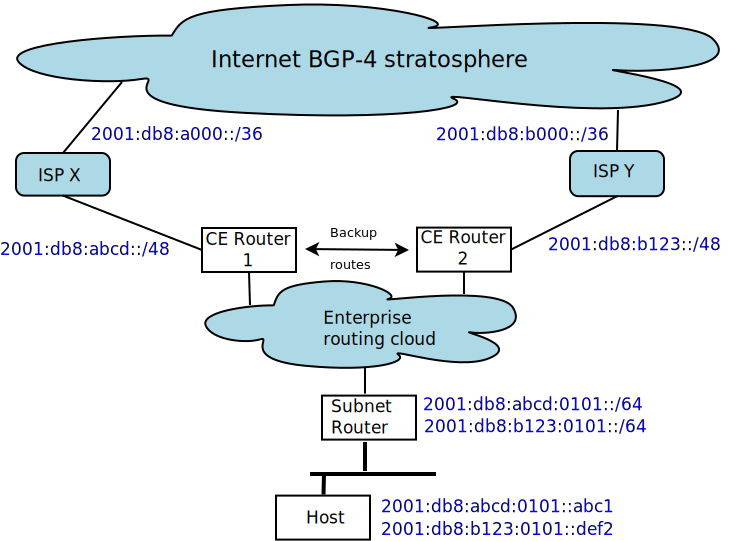
\includegraphics[keepaspectratio,alt={Routers and routing clouds as described above}]{multiPrefix.png}}
\caption{Routers and routing clouds as described above}
\end{figure}

If, for some reason, there is more than one subnet router on the subnet,
the host can be informed which one to use as suggested in
\href{https://www.rfc-editor.org/info/rfc8028}{RFC 8028}.

For this to work as intended, it is necessary to configure routing so
that traffic from \texttt{2001:db8:abcd:0101::abc1} exits the site
towards ISP X, and traffic from \texttt{2001:db8:b123:0101::def2} exits
towards ISP Y. Suitable source routing rules in the subnet router and
the rest of the enterprise routing cloud will do it. Such source routing
rules typically have to be set up as routing policies, including the
relevant source prefixes, configured on each router by a proprietary
mechanism.

But what happens if the link to ISP X goes down? Presumably the reason
for having two ISP connections is precisely for backup.

We can configure low priority (high metric) routes between the two exit
routers, such that when one ISP link is down, traffic is redirected to
the other. However, this may fail if the backup ISP applies ingress
filtering {[}\href{https://www.rfc-editor.org/info/bcp84}{BCP84}{]}, so
the enterprise needs to arrange for its ISPs to accept mutual backup
traffic.

If these steps (source routing \emph{and} backup routes \emph{and}
filtering exceptions) are not taken, a failure of one of the two ISP
connections will cause the failure of all user sessions using addresses
under that ISP\textquotesingle s PA prefix.

Even with backup routes in place, there may be a problem if user client
sessions originating \emph{within} the enterprise use IPv6 source
addresses under a failing PA prefix. This will happen unless the host is
somehow caused to deprecate such source addresses, so that the algorithm
of \href{https://www.rfc-editor.org/info/rfc6724}{RFC 6724} will not
select them.

An additional technique that has been suggested is for a site to deploy
\emph{conditional} router advertisements
{[}\href{https://www.rfc-editor.org/info/rfc8475}{RFC8475}{]}.

This whole topic is discussed in more depth in
\href{https://www.rfc-editor.org/info/rfc8678}{RFC 8678}.

The need for complex configuration and the resulting failure modes
explain why many enterprises have not opted for multi-prefix PA-based
multihoming. Instead, they have paid to obtain provider-independent (PI)
IPv6 prefixes, typically /48 in length, from an Internet registry.
However, this is expected to be problematic in the long term, since
every such enterprise adds to the size of the Internet-wide BGP-4
routing table. This may be viable for a few thousand enterprises, but
not for millions, i.e. not for small businesses or even home offices
that might benefit from multihoming.

At the time of writing, the most practical solution for multihoming with
multiple providers of IPv6 service (known as MHMP) remains under
discussion in the IETF.

Another use case for multiple prefixes is an enterprise (or home) that
in addition to its PA or PI prefix, which is routable anywhere on the
Internet, also decides to use a Unique Local Address (ULA) prefix for
strictly internal communication. Although unfamiliar to most operators,
this is conceptually simple and creates a class of traffic that \emph{by
definition} cannot escape the site, which has obvious privacy and
security attractions. Services that should only be accessed internally
could be configured with ULAs \emph{only} and those addresses may be
entered in local split-horizon DNS (Section 4 of
{[}\href{https://www.rfc-editor.org/info/rfc6950}{RFC6950}{]}). At the
time of writing, there is an operational problem in this scenario: host
computers configured with default settings from
\href{https://www.rfc-editor.org/info/rfc6724}{RFC 6724} will not prefer
ULAs over IPv4 addresses
{[}\href{https://datatracker.ietf.org/doc/draft-ietf-v6ops-ula/}{draft-ietf-v6ops-ula}{]}.
A site using DHCPv6 can change the default settings via
\href{https://www.rfc-editor.org/info/rfc7078}{RFC 7078}, but
unfortunately this is not widely implemented.

A partial work-around for this problem is for a host to have two AAAA
records in DNS, e.g. \texttt{www.example.com} for its GUA and
\texttt{w3.example.com} for its ULA, the latter only being present in
local split-horizon DNS.

\subsubsection{\texorpdfstring{\hyperref[security-operation]{Previous}
\hyperref[multihoming]{Next}
\hyperref[management-and-operations]{Top}}{Previous Next Top}}\label{previous-next-top-30}

\pagebreak

\subsection{Multihoming}\label{multihoming}

Multihoming means configuring a site in such a way that it is connected
via more than one link to the Internet, preferably via different ISPs,
usually to provide redundancy in case of failures. The phrase
"multihoming with multiple providers" (MHMP) is sometimes used.
\hyperref[multi-prefix-operation]{The previous section} describes the
problems in achieving MHMP using multiple address prefixes. This section
discusses practical techniques for site multihoming.

Domestic or very small office installations are out of scope for this
topic. They are rarely connected permanently to more than one ISP, and
therefore cannot expect smooth failover. They might have an alternative
connection (e.g., a wireless hot spot instead of a terrestrial
connection) but the changeover would amount to a network restart and
would likely be manual.

Note that the term "multihoming" is sometimes used to describe a
configuration \emph{inside} a site network where a node is connected to
more than one internal router to provide redundancy. That complicates
site routing, and is not the topic here.

In 2003, the IETF established goals for site multihoming
{[}\href{https://www.rfc-editor.org/info/rfc3582}{RFC3582}{]}. In
summary, the main goals were: redundancy, load sharing, performance,
policy control, simplicity, and transport session survivability. Without
describing all the efforts made since then, it is clear that a solution
that satisfies all these goals simultaneously has been difficult to
find. A more recent overview can be found in
\href{https://www.rfc-editor.org/info/rfc7157}{RFC 7157}.

\subsubsection{Large sites}\label{large-sites}

Today, the most practical approach for a large site, or for a large
enterprise network distributed over multiple physical sites, is to
obtain a provider-independent (PI) prefix from the appropriate Internet
address registry, which will typically be a /48 prefix such as
\texttt{2001:db8:face::/48}. Then all hosts in the enterprise network
that require Internet access will be assigned IPv6 addresses within that
prefix. They might also be assigned Unique Local Addresses (ULAs) for
internal use, or IPv4 addresses, or both. The enterprise will then
select at least two ISPs to provide redundant connectivity to the
Internet, and arrange for both of them to advertise a BGP-4 route to
that prefix.

A /48 prefix provides the theoretical capacity for more than 65 thousand
subnets. However, extremely large enterprises can obtain prefixes
shorter than /48 from one of the address registries, if they provide an
adequate technical justification.

Internal routing must be arranged to direct traffic as required, using
routing metrics that favor one ISP or another, or spread the load, as
desired. When the egress to a particular ISP fails, backup routes to an
alternative egress router will take over. An additional advantage to the
enterprise is that address renumbering will never be required, since the
/48 prefix is tied to the enterprise, not to one of their ISPs.

This method is tried and tested. However, there are two reasons why it
cannot be extended indefinitely to cover smaller enterprises or even
domestic users. Firstly, it is significantly more costly than a single
provider-assigned (PA) prefix, and requires some level of operational
management by skilled technicians. Secondly, the wide area BGP-4 routing
system is widely considered unable to cope with the millions of PI
prefixes that would ensue if a majority of small and medium enterprises
adopted this solution. In November 2023, the global BGP-4 system carried
about 200,000 IPv6 routes. There are estimated to be 32 million small
businesses in the USA alone, and 200 million in the world. If every
small business suddenly had its own PI prefix, the Internet would stop
working.

\subsubsection{Small or medium sites}\label{small-or-medium-sites}

Except for some thousands of large enterprises, a viable solution for
multihoming of small or medium enterprises must be based on PA
addresses, if it is to be used by millions of sites. However, as shown
in \hyperref[multi-prefix-operation]{the previous section}, operating
with more than one PA prefix at the same time is currently impractical,
especially if transport session survivability is required.

The IETF has made various attempts to solve this problem, including the
SHIM6 protocol
{[}\href{https://www.rfc-editor.org/info/rfc5533}{RFC5533}{]} and the
Multiple Provisioning Domain Architecture
{[}\href{https://www.rfc-editor.org/info/rfc7556}{RFC7556}{]}. Such
methods have not been successfully deployed. Other options, such as
centralizing redundant connections for a large corporate network at a
single site, or deploying application layer proxies to decouple internal
and external addressing, remain out of reach for small or medium
enterprises.

If we abandon the goal of transport session survivability, so that
applications will have to recover from broken transport connections
after a multihoming failover, the problem is simplified. It should be
noted that essentially all mass market client applications already
handle such disconnects, which are commonplace when mobile or portable
devices move from place to place. This leads to one possible approach to
multihoming for small sites, which is essentially to do nothing except
connect the site to two (or more) ISPs and assign two (or more) PA
prefixes, and leave client applications to find a working path by trial
and error. This is essentially a generalization of the Happy Eyeballs
approach {[}\href{https://www.rfc-editor.org/info/rfc8305}{RFC8305}{]},
but it will lead to help desk calls in the case of applications that are
not sufficiently resilient. It is clearly not sufficient for a large
site, especially if it operates servers as well as client hosts.

An approach that should avoid some of these help desk calls, but is not
currently favored by the IETF, is to use dynamic network prefix
translation, known as NPTv6
{[}\href{https://www.rfc-editor.org/info/rfc6296}{RFC6296}{]},
{[}\hyperref[translation-and-ipv4-as-a-service]{3. Translation and IPv4
as a service}{]}. In this model, a translator is placed at the site exit
router towards each ISP. Outgoing and incoming packets are translated to
and from appropriate PA addresses. The routeable prefix part of each
address is changed, and possibly some bits in the IID, in a way that
avoids transport checksum errors. This translation is stateless and
reversible, so causes much less difficulty than traditional NAT; no port
translation is needed.

To simplify the translation processs, internal hosts (both clients and
servers) would be assigned Unique Local Addresses (ULAs)
{[}\href{https://www.rfc-editor.org/info/rfc4193}{RFC4193}{]} that would
rarely change. However, servers will be announced to the outside world
via DNS using their translated PA addresses.

This method is known to have been successfully tested, although not
recommended by the IETF. It should be noted, however, that NPTv6 does
not share all the disadvantages of IPv4 NAT. As discussed in RFC 6296,

\begin{itemize}
\item
  NPTv6 does not need to translate port numbers, and it is
  checksum-neutral, so the transport layer is effectively unaffected.
\item
  Translation is stateless, so matters such as asymmetric routing, load
  sharing, and router fail-over are not affected.
\item
  Filtering of unwanted traffic requires an adequate firewall, but this
  is true for any serious IPv6 (or IPv4) deployment.
\item
  Topology hiding, which is sometimes cited as an argument for NAT, is
  discussed in {[}\hyperref[topology-obfuscation]{4. Topology
  obfuscation}{]}. NPTv6 does indeed largely obfuscate local topology.
  For example (again following RFC 6296), a host whose actual address is
  \texttt{fd01:0203:0405:0001::1234} might appear on the Internet as
  \texttt{2001:db8:0001:d550::1234}. An attacker that does not know the
  site\textquotesingle s ULA prefix (\texttt{fd01:0203:0405::/48})
  cannot reverse the translation and deduce the actual subnet prefix.
\end{itemize}

Of course, NPTv6 retains some of the disadvantages of NAT: all of the
problems that directly follow from having different IP addresses at the
two ends of a connection. Section 5 of
\href{https://www.rfc-editor.org/info/rfc6296}{RFC 6296} discusses this.
Any site running NPTv6 must either deal with these problems, or avoid
any affected applications. In particular, SIP (Session Initiation
Protocol for IP telephony) will not work without the support of a proxy
mechanism {[}\href{https://www.rfc-editor.org/info/rfc6314}{RFC6314}{]}
as well as provision for IPv6/IPv4 coexistence
{[}\href{https://www.rfc-editor.org/info/rfc6157}{RFC6157}{]}. This
limits the applicability of NPTv6.

\subsubsection{Transport layer
solutions}\label{transport-layer-solutions}

Another possible approach to site multihoming is to treat it as a
transport layer problem. If a transport protocol is agile enough to use
multiple paths (i.e., multiple source/destination address pairs),
failures at the network layer can be hidden. Multipath TCP (MPTCP,
{[}\href{https://www.rfc-editor.org/info/rfc8684}{RFC8684}{]}) is
defined but not widely available. A multipath version of QUIC is under
discussion, as is a versatile API for the transport layer that would
support multipath solutions. Discussion continues in the IETF.

\subsubsection{\texorpdfstring{\hyperref[multi-prefix-operation]{Previous}
\hyperref[energy-consumption]{Next}
\hyperref[management-and-operations]{Top}}{Previous Next Top}}\label{previous-next-top-31}

\pagebreak

\subsection{Energy consumption}\label{energy-consumption}

There is no firm evidence whether IPv6 has net energy consumption
greater or less than IPv4 for the same application layer traffic load.
There are factors that might work in favour of IPv6, such as a larger
minimum PDU size or less energy spent on network address translation,
and factors that might work against it, such as the transmission time
for longer packet headers or greater use of link-local multicast.
Equally, there is no evidence whether different co-existence strategies
(e.g., native dual stack versus IPv4-as-a-service) have significantly
different energy costs.

\href{https://www.rfc-editor.org/info/bcp202}{BCP 202} makes specific
recommendations on reducing the energy consumption of IPv6 Router
Advertisements.

It is worth noting that in the area of constrained IPv6 nodes with very
limited battery power and transmission capacity
{[}\href{https://www.rfc-editor.org/info/rfc8376}{RFC8376}{]},
considerable attention has been paid to energy consumption, including
compression mechanisms such as Generic Framework for Static Context
Header Compression and Fragmentation (SCHC)
{[}\href{https://www.rfc-editor.org/info/rfc8724}{RFC8724}{]}.

\subsubsection{\texorpdfstring{\hyperref[multihoming]{Previous}
\hyperref[packet-size-and-jumbo-frames]{Next}
\hyperref[management-and-operations]{Top}}{Previous Next Top}}\label{previous-next-top-32}

\pagebreak

\subsection{Packet size and Jumbo
Frames}\label{packet-size-and-jumbo-frames}

\subsubsection{Fragmentation}\label{fragmentation}

As already stated in \hyperref[ipv6-primary-differences-from-ipv4]{3.
IPv6 primary differences from IPv4}, IPv6 does not allow intermediate
routers to fragment packets. Instead, IPv6 pushes the responsibility of
fragmentation to the source node. If a packet exceeds the MTU, it is
either fragmented by the sender or dropped. This means the sender must
use PMTUD {[}\href{https://www.rfc-editor.org/info/rfc7690}{RFC7690}{]}
to ensure that packets are sized appropriately for the smallest MTU
along the path. The sender fragments packets if necessary before sending
them. This require additional computation on the sender to fragment
packets but there has been no significant performance implication
reported.

\subsubsection{MTU Size and Jumbo
Frames}\label{mtu-size-and-jumbo-frames}

A jumbo frame is an Ethernet frame that is larger than the standard 1500
bytes, commonly configured to be around 9000 bytes. If a router along
the path has a smaller MTU when sending jumbo frames in an IPv4 network,
it will fragment the frame. This can lead to higher fragmentation
overhead because the larger the original frame, the more fragments it
must be split into. Additionally, fragmentation adds processing
complexity at both the router and the destination where reassembly
occurs.

IPv6 avoids this fragmentation overhead by relying on PMTUD
{[}\href{https://www.rfc-editor.org/info/rfc7690}{RFC7690}{]}. If a
jumbo frame exceeds the MTU of any network hop, the sender is
responsible for fragmenting it before transmission. However, if properly
configured, the sender can send larger packets efficiently without
fragmentation, provided that the entire path supports jumbo frames. Ths
allows IPv6 to handle larger packets more effectively because the Path
MTU Discovery mechanism ensures that packets fit within the MTU of every
hop along the route. This mechanism is defined in
{[}\href{https://www.rfc-editor.org/info/rfc8201}{RFC8201}{]}.

The ``Jumbo Payload Option'' in IPv6
{[}\href{https://www.rfc-editor.org/info/rfc2675}{RFC2675}{]} allows
packets larger than 65,535 bytes (the maximum payload size for standard
IPv6 packets) to be transmitted. This option is included in the
Hop-by-Hop Options header and enables IPv6 to support super jumbo frames
efficiently, even when dealing with extremely large packet sizes. This
mechanism simplifies the handling of large packets without requiring
them to be split into smaller fragments. If a network supports large
enough MTUs, IPv6 can use this option to transmit large frames without
intermediate fragmentation. However, it is very little used because it
needs a layer 2 technology supporting very big packets. An interesting
use case is for \emph{internal} communication in support of segmentation
offload, described in
\href{https://www.sipanda.io/post/segmentation-offload-and-protocols-let-s-be-friends}{this
blog entry}.

\subsubsection{\texorpdfstring{\hyperref[energy-consumption]{Previous}
\hyperref[basic-windows-commands]{Next}
\hyperref[management-and-operations]{Top}}{Previous Next Top}}\label{previous-next-top-33}

\pagebreak

\subsection{Basic Windows commands}\label{basic-windows-commands}

To determine current IPv6 configuration, type \texttt{ipconfig\ /all} at
the Windows command prompt.

Both \texttt{ping} and \texttt{tracert} work normally for IPv6. In the
case of link-local addresses, Windows supports the default zone
identifier (also known as the default interface), so
\texttt{ping\ fe80::1234} will automatically use the default interface.
On a host with more than one network interface, the interface may be
specified, e.g. \texttt{ping\ fe80::1234\%7}. The interfaces in use can
be found in the output from \texttt{ipconfig\ /all}.

To check basic IPv6 configuration, use
\texttt{Control\ Panel/All\ Control\ Panel\ Items/Network\ and\ Sharing\ Center/Change\ Adapter\ Settings}.
Select the network adapter of interest, then
\texttt{Properties/Internet\ Protocol\ Version\ 6} and basic properties
will be available. Normally, nothing will need to be changed.

More advanced properties can be checked or changed from the command
prompt with \texttt{netsh}, e.g.,
\texttt{netsh\ interface\ ipv6\ show\ privacy} to show whether temporary
addresses are active. Since \texttt{netsh} is a very complex tool, we do
not fully describe it here, but it includes on-line help at every level,
by adding \texttt{?} to a command, e.g.,
\texttt{netsh\ interface\ ipv6\ show\ interfaces\ ?}.

The same functionality (and more) is also available using PowerShell,
for which we suggest seeking Microsoft documentation.

\subsubsection{\texorpdfstring{\hyperref[packet-size-and-jumbo-frames]{Previous}
\hyperref[case-studies]{Next}
\hyperref[management-and-operations]{Top}}{Previous Next Top}}\label{previous-next-top-34}

\pagebreak

\section{Case Studies}\label{case-studies}

This chapter will contain a variety of short case studies, based on real
experience, for a range of network types. It will never be complete, as
every network is slightly different, and it will evolve as time goes on.

A good set of existing case studies from ARIN members can be found in
\href{https://www.arin.net/blog/ipv6/}{the ARIN blog}.

Here is a Malaysian case study via
\href{https://blog.apnic.net/2023/03/17/telekom-malaysias-ipv6-readiness-journey/}{APNIC}.

Here is a deployment case
\href{https://nsrc.org/blog/apricot-ipv6-only}{at a large conference}.

This is an \textbf{open invitation} to contribute a case study for this
chapter. If you have deployed an IPv6 network, please write a short
section with emphasis on what major choices you made, what worked well,
and what problems you encountered. Even a summary in one paragraph would
be helpful. Large and small enterprise networks, and large or small
carrier networks, are all of interest. It isn\textquotesingle t
necessary to identify the particular network, if you prefer to keep that
private.

If you have already published such a description, just a pointer will be
fine.

\href{https://github.com/becarpenter/book6/blob/main/1.\%20Introduction\%20and\%20Foreword/How\%20to\%20contribute.md\#how-to-contribute}{How
to contribute}

\hyperref[cern-and-the-lhc]{CERN and the LHC}

\subsubsection{\texorpdfstring{\hyperref[list-of-contents]{Back to main
Contents}}{Back to main Contents}}\label{back-to-main-contents-6}

\pagebreak

\subsection{CERN and the LHC}\label{cern-and-the-lhc}

The \href{https://www.cern.ch}{CERN laboratory} and the
\href{https://home.cern/science/computing/grid}{Worldwide Large Hadron
Collide Computing Grid (WLCG)} are large users of IPv6 for massive data
transfers. Some statistics from early 2024 are shown here:

\begin{figure}
\centering
\pandocbounded{\includegraphics[keepaspectratio,alt={Graph showing 644 Gb/s}]{CERN-IPv6-Feb24.png}}
\caption{Graph showing 644 Gb/s}
\end{figure}

(Image from the February 2024 data challenge at CERN.)

The CERN site itself operates a classical IPv4 and IPv6 dual stack, and
uses DHCPv6 for IPv6 address assignment.

A detailed report on progess towards IPv6-only in the WLCG can be found
\href{https://docs.google.com/presentation/d/1riTdi7zgoJ3ig31Hp-gy4Z089PeKaoRJHALOcvjGn5E/}{here}.

\subsubsection{\texorpdfstring{\hyperref[deployment-status]{Next}
\hyperref[case-studies]{Top}}{Next Top}}\label{next-top-6}

\pagebreak

\section{Deployment Status}\label{deployment-status}

This chapter outlines information about IPv6 deployments. The picture
changes daily, so what follows is very likely to be out of date.

For information about product support for IPv6 features, users might be
interested by the University of New Hampshire
\href{https://www.iol.unh.edu/testing/ipv6}{InterOperability
Laboratory}, the NIST
\href{https://www.nist.gov/programs-projects/usgv6-program}{USGv6
Program}, or the \href{https://www.ipv6ready.org/}{IPv6 Ready Logo
Program}.

\hyperref[status]{Status}

\hyperref[deployment-by-carriers]{Deployment by carriers}

\hyperref[deployment-in-the-home]{Deployment in the home}

\hyperref[deployment-in-the-enterprise]{Deployment in the enterprise}

\subsubsection{\texorpdfstring{\hyperref[list-of-contents]{Back to main
Contents}}{Back to main Contents}}\label{back-to-main-contents-7}

\pagebreak

\subsection{Status}\label{status}

When speaking of IPv6, a question immediately comes up: "How many people
currently use IPv6 on the Internet?". Answering this question is
fundamental to gain an understanding of the real adoption of IPv6. A
2023 overview is presented in
\href{https://www.rfc-editor.org/info/rfc9386}{RFC 9386}.

A count of IPv6 users is monitored by various organizations. For
example, both
\href{https://www.facebook.com/ipv6/?tab=ipv6_total_adoption}{Facebook}
and \href{https://www.google.com/intl/en/ipv6/statistics.html}{Google}
provide statistics on the users that access their services over IPv6.
The results are different, due to different methods being used. Google
generally sees more IPv6 usage than Facebook, but Google has a blind
spot in China where adoption is significant.

A trusted source from a Regional Internet Registry (RIR) is
\href{https://stats.labs.apnic.net/ipv6/}{APNIC Labs}. This site
measures \emph{capability} rather than traffic or active users, so the
data should not be directly compared with Google or Facebook. APNIC
quantifies the availability of IPv6 by means of a script that runs on
Internet browsers.

A very informative blog was posted in 2023 by
\href{https://blog.cloudflare.com/ipv6-from-dns-pov}{Cloudflare},
showing that humans use IPv6 a lot more than bots, which seem to prefer
IPv4. Cloudflare\textquotesingle s current protocol usage data is
summarized by \href{https://radar.cloudflare.com/}{Cloudflare radar}.

\href{https://web.archive.org/web/20250324111641/https://www.akamai.com/internet-station/cyber-attacks/state-of-the-internet-report/ipv6-adoption-visualization}{Akamai}
formerly provided data measuring the number of hits to their content
delivery platform. For example, they showed 72\% adoption in India in
early 2024.

In late 2025, Google, Facebook and Cloudflare roughly agreed on 40 to
50\% worldwide adoption by users, with APNIC Labs showing 42\% IPv6
capability.

Some statistics on DNS records and reachability for top web sites may be
found at \href{https://www.employees.org/~dwing/aaaa-stats/}{Dan
Wing\textquotesingle s site}. These data suggest that only 30\% of sites
had IPv6 DNS entries by November 2025. So while major sites are seeing
up to 50\% IPv6 usage, most smaller sites are not even in the game.

At the time of writing, there are significant discrepancies between data
from these and other sources. In fact there is no well-defined metric
for "how many IPv6 users exist" or "how much IPv6 traffic exists". To
take one example, Google estimates the fraction of Google "hits" that
use IPv6, yet Google is very little used in China so these data cannot
represent the true world-wide situation. Estimates posted to the IETF by
Geoff Huston in July 2023 suggested that Google then observed a 7\%
adoption rate in China, while the APNIC measurement reported 30\%
capability.

We show here an older APNIC presentation of results to show the number
of the Internet IPv6 users some years ago, compared with the total
Internet population (in millions, see next table).

\begin{figure}
\centering
\pandocbounded{\includegraphics[keepaspectratio,alt={Table shows 25\% annual IPv6 growth 2018 to 2022}]{Section5_Table1.jpg}}
\caption{Table shows 25\% annual IPv6 growth 2018 to 2022}
\end{figure}

A third of the Internet population apparently employed IPv6 then. It is
also interesting to look at the growth curve. The main indicator here is
the Compound Annual Growth Rate (CAGR), which shows a two-digit growth
across the 5-year period 2018-2022.

There is a caveat, however. The method used by APNIC cannot be fully
employed in China, due to local policy filtering traffic from abroad. An
independent
\href{https://www.china-ipv6.cn/\#/activeconnect/simpleInfo}{Chinese
research} reported 713 million measured IPv6 customers as of September
2022, against the 220 million reported by APNIC. If we added the
difference between the two statistics to the global count, we would end
up with a usage of 43\% in September 2022. (As it happened, the Google
worldwide measurement in that month peaked at 41\%.)

In August 2025, China's Cyberspace Administration announced that by
June, China had 834 million active IPv6 users, i.e., 75\% of Chinese
Internet users. 66\% of traffic on mobile networks ran over IPv6, vs
28\% on fixed networks. By October 2025,
\href{https://www.chinadaily.com.cn/a/202510/31/WS690473f6a310f735438b8167.html}{Chinese
media claimed 77\% adoption}.

\subsubsection{\texorpdfstring{\hyperref[deployment-by-carriers]{Next}
\hyperref[deployment-status]{Top}}{Next Top}}\label{next-top-7}

\pagebreak

\subsection{Deployment by carriers}\label{deployment-by-carriers}

All the organizations providing or using Internet connectivity services
have an associated Autonous System Number (ASN).
\href{https://blog.apnic.net/2022/01/06/bgp-in-2021-the-bgp-table/}{APNIC}
provides statistics on the evolution of IPv6 support across the ASNs in
the world, as observed in the Internet routing tables.

\begin{figure}
\centering
\pandocbounded{\includegraphics[keepaspectratio,alt={Table shows 18\% annual IPv6 growth 2018 to 2022}]{Section5_Table2.jpg}}
\caption{Table shows 18\% annual IPv6 growth 2018 to 2022}
\end{figure}

The percentage of IPv6-capable ASNs is growing over the years, which is
a good sign. On the other hand, the table does not distinguish the
degree of adoption across the different industries, that is whether the
ASNs are associated to a carrier, a service provider or an entreprise.
To zoom in at that level, it is necessary to look at more detailed
statistics such as those provided by
\href{https://www.akamai.com/internet-station/cyber-attacks/state-of-the-internet-report/ipv6-adoption-visualization}{Akamai}
or \href{https://stats.labs.apnic.net}{APNIC}.

Not unsurprisingly, the vast majority of carriers worldwide already
support IPv6. Yet, differences exist. As a general rule, the carriers
active in those countries with higher IPv6 adoption also show higher
levels of IPv6 utilization. For example, based on the Akamai statistics,
IPv6 adoption in the United States is 51\%. Carriers such as AT\&T,
Comcast, T-Mobile and Verizon all exceed 70\% of IPv6 use in their
networks. In Europe, both Belgium and Germany reach 50\% of IPv6
traffic. Proximus, Telenet, DT, Telefonica Germany, Versatel and
Vodafone Germany range from 50\% to 70\%. India shows 51\% IPv6
adoption. Carriers there also have a high IPv6 rate. Bharti, Reliance
Jio and Vodafone India find themselves between 60\% and 70\%.

Whilst it cannot be gneralized, in countries with lower IPv6 adoption
the local carriers also tend to be slower in enabling IPv6. For example,
European countries such as Spain, Italy and Poland show respectively
4.5\%, 7\% and 13.5\% adoption. Based on APNIC data, exluding the
exceptions of Telefonica de España (26\%), Vodafone Italy (21\%), Wind/3
Italy (22\%) and Orange Poland (23\%), all the other carries sit quite
below the threshold of 20\% adoption.

Differences also apply between wired and wireless carriers. The latter
are often more advanced with IPv6. In several cases
{[}\href{https://www.rfc-editor.org/info/rfc9386}{RFC9386}{]}, the
reason for them to move to IPv6 depended on the lack of public IPv4
addresses. Those carriers have decided to develop strategic plans to
enable IPv6-only underlay services, for example through the adoption of
translation mechanisms such as 464XLAT (Reliance Jio, T-Mobile),
guaranteeing legacy IPv4-as-a-Service support. Notable examples of early
IPv6 adoption in the wired domain are Comcast in the US and Sky in the
UK.

\subsubsection{\texorpdfstring{\hyperref[status]{Previous}
\hyperref[deployment-in-the-home]{Next}
\hyperref[deployment-status]{Top}}{Previous Next Top}}\label{previous-next-top-35}

\pagebreak

\subsection{Deployment in the home}\label{deployment-in-the-home}

It is hard to estimate what fraction of home users have IPv6
connectivity on a given date. The
\href{https://www.google.com/intl/en/ipv6/statistics.html}{Google}
statistics are interesting, because they clearly show weekend peaks in
IPv6 access (up to 43\% in April 2023), suggesting a quite high level of
home and/or mobile IPv6 connectivity.

Some, but not all, devices on the market for home (or small office) use
support both IPv6 and IPv4. However, older devices only have IPv4. For
this reason, a typical home network today runs a dual stack. Also, a
typical network does not include multiple subnets; the only router
present is at the same time the subnet router and the CE router.
Assuming the ISP supports IPv6, regardless whether it provides native
IPv4 or IPv4 as a service, the router provides a dual stack service on
the LAN. The LAN itself is typically WiFi, possibly bridged to Ethernet.
(Even if the CE router does \emph{not} support IPv6 at all, link-local
IPv6 should work.)

As a result, things are fairly simple. Devices such as PCs and printers
can communicate with each other using whatever works -\/- IPv4,
link-local IPv6, or global IPv6. (For example: a Windows 10 PC installed
in 2019 communicates with a Canon inkjet printer installed in 2022,
using link-local IPv6, needing no manual configuration.) Connections to
the Internet will be preferentially established using IPv6 for services
that have a AAAA address in the DNS, or IPv4 otherwise. Such connections
may be optimized by the Happy Eyeballs technique
{[}\href{https://www.rfc-editor.org/info/rfc8305}{RFC8305}{]}. Most home
users will remain largely ignorant of all this.

The situation becomes more complicated when various home automation
devices are considered, especially if it becomes desirable to split the
home network into separate subnets. Such networks need to be essentially
self-configuring and self-managing, as do "Internet of Things" networks.
These complex topics are out of scope for this book.

\subsubsection{\texorpdfstring{\hyperref[deployment-by-carriers]{Previous}
\hyperref[deployment-in-the-enterprise]{Next}
\hyperref[deployment-status]{Top}}{Previous Next Top}}\label{previous-next-top-36}

\pagebreak

\subsection{Deployment in the
enterprise}\label{deployment-in-the-enterprise}

Measuring the adoption of IPv6 in the enterprise domain is not
straightforward. Since it is hard to look at it from the network
"inside", one of the few currently available approaches is to check the
IPv6 readiness from outside the enterprise\textquotesingle s network.
\href{https://fedv6-deployment.antd.nist.gov/cgi-bin/generate-com}{NIST}
provides a method to infer whether US enterprises support IPv6 by
checking its external services, such as the availability of Domain Name
System (DNS) AAAA records, an IPv6-based mail service, or the support of
IPv6 on their website. The same method can be applied to
\href{http://218.2.231.237:5001/cgi-bin/generate}{Chinese} and
\href{https://cnlabs.in/IPv6_Mon/generate_industry.html}{Indian}
enterprises.

DNS has a good support in all cases: more than 50\% of the enterprises
in the three economies considered have AAAA records, a sign that IPv6
support is generally available. The same cannot be said of the other
services that have much lower adoption.
{[}\href{https://www.rfc-editor.org/info/rfc9386}{RFC9386}{]} provides
other statistics about more specific industry domains.

What are the factors hindering the adoption of IPv6 in the enterprise?
Appendix B of
{[}\href{https://www.rfc-editor.org/info/rfc9386}{RFC9386}{]} reports
the result of a poll issued by the
\href{https://industrynetcouncil.org/}{Industry Network Technology
Council (INTC)} to check the need for IPv6 training by some medium and
large US enterprises.

The poll shows that lack of IPv6 knowledge is one of the main issues.
This reflects into the need for training, in particular in the areas of
IPv6 security and IPv6 troubleshooting. Apart from training, enterprises
feel that IPv6 security is of operational concern as well as the
conversion of the applications they use in their daily activity to IPv6.

\subsubsection{Addressing in the
enterprise}\label{addressing-in-the-enterprise}

How organizations craft their addressing schemes will be varied and will
likely be determined by a number of factors. The largest factor that
will influence the procurement or otherwise obtaining of address
resources will be organizational size. The size of a given organization
often (but not always) dictates the criticality of networking resources
which includes both physical assets (routers, switches, security
appliances) as well as human resources, and the level of skill available
either by direct employment or by contracted assistance. Also included
in these resources is the logical elements required for a presence on
the global internet in the manner of addressing. Larger or more mature
organizations may already posses network resources such as Autonomous
System Numbers (ASNs), legacy IP resources, and possibly existing
provider independent (PI) IPv6 space. First, it is important to make the
distinction of address space types. There are really three different
types of address allocations possible, provider independent, provider
allocated, and unique local addressing {[}\hyperref[addresses]{2.
Addresses}{]}.

Organizations will need to understand the differences as it will be both
dictated by resource availability and will inform routing policy and
future deployment changes.

\textbf{Provider Independent address space}

Provider Independent (PI) address space consists of address resources
obtained directly from a regional internet registry (RIR). These address
resources are allocated to a requesting entity after a formal request
process that entails a light justification process and an annual fee
collection. The addressing is allocated to the requesting entity and,
within the scope of the global internet best practices, can be used
however the assigned entity sees fit.

For PI address space based deployments, organizations will need to
contract external consultancy or have in-house expertise in obtaining
address space from a regional internet registry (RIR) that will be
determined by the locality of their organization. Further, obtaining PI
address space from an RIR means coordinating with their ISP(s) to route
the PI space based on some routing policy with upstream provider(s). If
an organization is not staffed to or does not have the experience or
knowledge on the processes of obtaining address space and routing it
globally (i.e. within the internet default free zone (DFZ)), it will be
required to contract such tasks. In house or contracted IT support
should understand the intricacies of routing policy of said PI address
space in the appropriate routing registries, maintaining best practice
filtering (MANRS), populating and maintaining internet route registry
(IRR) data, implementing Resource Public Key Infrastructure (RPKI), and
have at least a rudimentary understanding of what operating in the DFZ
means. In general, maintaining PI address space offers the most
flexibility and stability due to the portable nature of the resources,
and although it does have a higher startup cost both operationally and
financially, is the preferable method for medium to large enterprises.

\textbf{Provider Assigned address space}

Provider Assigned (PA) address space consists of address space that is
assigned to a specific upstream provider and sub-delegated to a
customer.

If receiving PA from an upstream provider, designs such as multihoming
is a more involved process that will involve coordination with the
upstream transit provider that owns the IP resources. (See
{[}\hyperref[multi-prefix-operation]{6. Multi-prefix operation}{]} for
some discussion of multihoming.) Additionally, renumbering is
functionally required if said provider is exchanged for another unless
NAT is employed as a translation tool. Obtaining additional address
space may require more effort and expense, or may not be possible.

\subsubsection{\texorpdfstring{\hyperref[deployment-in-the-home]{Previous}
\hyperref[troubleshooting]{Next}
\hyperref[deployment-status]{Top}}{Previous Next Top}}\label{previous-next-top-37}

\pagebreak

\section{Troubleshooting}\label{troubleshooting}

Troubleshooting IPv6 issues involves following established best
practices used broadly in network troubleshooting methodologies:

\begin{enumerate}
\def\labelenumi{\arabic{enumi}.}
\tightlist
\item
  \textbf{Observe Behavior:} Clearly define and document the unexpected
  or undesirable network behavior.
\item
  \textbf{Compare Against Baseline:} If available, compare the current
  state to a previously established and documented baseline.
\item
  \textbf{Document Changes:} Maintain accurate records of network
  configurations and any modifications.
\item
  \textbf{Make Simple, Single Changes:} Implement changes one at a time
  to isolate variables effectively.
\item
  \textbf{Repeat:} Continue iterating the process until the issue is
  resolved.
\end{enumerate}

Due to their similarities, IPv4 troubleshooting techniques are highly
transferable to IPv6, given that both protocols are routed, support
various services, run on hosts and networking devices, and facilitate
management traffic.

\subsection{Troubleshooting Layer 2
Communications}\label{troubleshooting-layer-2-communications}

Layer 2 troubleshooting for IPv6 involves ensuring basic connectivity at
the data link layer, including:

\begin{itemize}
\item
  \textbf{Address Resolution:} Verify the proper functioning of Neighbor
  Discovery Protocol (NDP), as IPv6 does not use ARP. Common commands
  include:

\begin{Shaded}
\begin{Highlighting}[]
\CommentTok{\# Display IPv6 neighbors}
\ExtensionTok{ip} \AttributeTok{{-}6}\NormalTok{ neigh}
\end{Highlighting}
\end{Shaded}
\item
  \textbf{Check Link-Local Connectivity:} Confirm local communication
  using link-local addresses. This isolates problems to the local
  segment.

\begin{Shaded}
\begin{Highlighting}[]
\CommentTok{\# Ping using link{-}local addresses}
\ExtensionTok{ping6}\NormalTok{ fe80::}\OperatorTok{\textless{}}\NormalTok{interface{-}id}\OperatorTok{\textgreater{}}\NormalTok{\%}\OperatorTok{\textless{}}\NormalTok{interface{-}name}\OperatorTok{\textgreater{}}
\end{Highlighting}
\end{Shaded}
\item
  \textbf{Multicast Listener Discovery (MLD):} Ensure multicast
  listeners are operational, as NDP relies heavily on multicast.
\end{itemize}

\subsection{Troubleshooting Layer 3
Communications}\label{troubleshooting-layer-3-communications}

Layer 3 troubleshooting involves validating routing and reachability of
IPv6 networks:

\begin{itemize}
\item
  \textbf{IPv6 Routing Table:} Inspect the routing table for correct and
  complete entries.

\begin{Shaded}
\begin{Highlighting}[]
\CommentTok{\# Display IPv6 routing table}
\ExtensionTok{ip} \AttributeTok{{-}6}\NormalTok{ route}
\end{Highlighting}
\end{Shaded}
\item
  \textbf{ICMPv6 Diagnostics:} Use ICMPv6 tools like ping6 and
  traceroute6 to verify end-to-end connectivity and path determination.

\begin{Shaded}
\begin{Highlighting}[]
\ExtensionTok{ping6}\NormalTok{ 2001:db8::1}
\ExtensionTok{traceroute6}\NormalTok{ 2001:db8::1}
\end{Highlighting}
\end{Shaded}
\item
  \textbf{Service Availability:} Validate that network services (DNS,
  DHCP, web services) respond correctly for both IPv4 and IPv6 requests.

\begin{Shaded}
\begin{Highlighting}[]
\ExtensionTok{dig}\NormalTok{ A example.com}
\ExtensionTok{dig}\NormalTok{ AAAA example.com}
\end{Highlighting}
\end{Shaded}
\item
  \textbf{Performance Baselines:} Continuously monitor dual-stack
  performance to detect and remediate suboptimal IPv6 connectivity.
\end{itemize}

\subsection{Happy Eyeballs Algorithm}\label{happy-eyeballs-algorithm}

The "Happy Eyeballs" algorithm (RFC 8305) optimizes dual-stack
experiences by dynamically choosing the protocol that provides the best
user experience:

\begin{itemize}
\tightlist
\item
  \textbf{Behavior Analysis:} Observe connections initiated by the
  application and verify if it appropriately falls back to IPv4 when
  IPv6 connectivity is poor or fails.
\item
  \textbf{Timeout Adjustments:} Tune timers within applications to
  optimize the balance between IPv4 fallback speed and IPv6 preference.
\item
  \textbf{Diagnostic Tools:} Utilize browser developer tools or packet
  captures (Wireshark, tcpdump) to monitor application behavior in
  real-time.
\end{itemize}

Effective IPv6 troubleshooting ensures that modern networks operate
efficiently, leveraging the advantages of IPv6 while maintaining a
seamless transition from IPv4.

\hyperref[advanced-troubleshooting]{Advanced Troubleshooting}

\hyperref[tools]{Tools}

\subsubsection{\texorpdfstring{\hyperref[list-of-contents]{Back to main
Contents}}{Back to main Contents}}\label{back-to-main-contents-8}

\pagebreak

\subsection{Advanced Troubleshooting}\label{advanced-troubleshooting}

\begin{itemize}
\item
  \textbf{Multicast Listener Discovery (MLD):} Ensure multicast
  listeners are operational, as NDP relies heavily on multicast.
\item
  \textbf{Firewall and ACL Verification:} Ensure that firewalls or
  access control lists (ACLs) permit necessary IPv6 traffic.
\end{itemize}

Firewall policy should match between protocols wherever possible. ICMPv6
is a notable exception, due to the significant differences and notable
reliance on ICMPv6 for normal IPv6 function.

\subsubsection{Troubleshooting Dual-Stack
Networks}\label{troubleshooting-dual-stack-networks}

In dual-stack environments, it is crucial to address complexities
stemming from simultaneous IPv4 and IPv6 operation:

\begin{itemize}
\item
  \textbf{Protocol Preference Issues:} Identify cases where applications
  or hosts may incorrectly prefer IPv4 over IPv6, or vice versa.

\begin{Shaded}
\begin{Highlighting}[]
\CommentTok{\# Check routing preference}
\FunctionTok{getent}\NormalTok{ ahosts example.com}
\end{Highlighting}
\end{Shaded}
\item
  \textbf{Service Availability:} Validate that network services (DNS,
  DHCP, web services) respond correctly for both IPv4 and IPv6 requests.

\begin{Shaded}
\begin{Highlighting}[]
\ExtensionTok{dig}\NormalTok{ A example.com}
\ExtensionTok{dig}\NormalTok{ AAAA example.com}
\end{Highlighting}
\end{Shaded}
\item
  \textbf{Performance Baselines:} Continuously monitor dual-stack
  performance to detect and remediate suboptimal IPv6 connectivity.
\end{itemize}

\subsubsection{Happy Eyeballs
Algorithm}\label{happy-eyeballs-algorithm-1}

The "Happy Eyeballs" algorithm (RFC 8305) optimizes dual-stack
experiences by dynamically choosing the protocol that provides the best
user experience:

\begin{itemize}
\tightlist
\item
  \textbf{Behavior Analysis:} Observe connections initiated by the
  application and verify if it appropriately falls back to IPv4 when
  IPv6 connectivity is poor or fails.
\item
  \textbf{Timeout Adjustments:} Tune timers within applications to
  optimize the balance between IPv4 fallback speed and IPv6 preference.
\item
  \textbf{Diagnostic Tools:} Utilize browser developer tools or packet
  captures (Wireshark, tcpdump) to monitor application behavior in
  real-time.
\end{itemize}

\subsubsection{Troubleshooting Translation
Mechanisms}\label{troubleshooting-translation-mechanisms}

\textbf{DNS64}\\
Verify DNS64 functionality by ensuring AAAA record synthesis for
IPv4-only services. Monitor responses with:

\begin{Shaded}
\begin{Highlighting}[]
\ExtensionTok{dig}\NormalTok{ AAAA ipv4{-}only{-}domain.example}
\end{Highlighting}
\end{Shaded}

\textbf{NAT64}\\
Confirm NAT64 translations with state tables and packet captures to
verify proper address and port mappings.

\begin{Shaded}
\begin{Highlighting}[]
\CommentTok{\# Inspect NAT64 mappings}
\ExtensionTok{show}\NormalTok{ nat64 translations}
\end{Highlighting}
\end{Shaded}

\textbf{pref64}\\
Check prefix discovery mechanisms used by hosts to determine NAT64
prefix.

\begin{Shaded}
\begin{Highlighting}[]
\ExtensionTok{ip} \AttributeTok{{-}6}\NormalTok{ route show}
\end{Highlighting}
\end{Shaded}

\subsubsection{IPv6-only Networks}\label{ipv6-only-networks}

Validate services and applications compatibility in IPv6-only
environments. Test DNS, DHCPv6, and ensure no IPv4 dependencies remain:

\begin{Shaded}
\begin{Highlighting}[]
\ExtensionTok{ping6}\NormalTok{ ipv6{-}only{-}host.example}
\end{Highlighting}
\end{Shaded}

\subsubsection{Multicast Issues}\label{multicast-issues}

\textbf{Wireless and Wireless Controllers}\\
Ensure multicast traffic is permitted and configured correctly on
wireless controllers to support IPv6 multicast applications.

\textbf{Router Advertisement Issues}\\
Check proper Router Advertisement (RA) dissemination, ensuring routers
advertise correct prefixes and default routes:

\begin{Shaded}
\begin{Highlighting}[]
\ExtensionTok{tcpdump} \AttributeTok{{-}i}\NormalTok{ eth0 icmp6 and ip6}\PreprocessorTok{[}\SpecialStringTok{40}\PreprocessorTok{]}\NormalTok{ == 134}
\end{Highlighting}
\end{Shaded}

\subsubsection{Host-Based Firewalls}\label{host-based-firewalls}

Inspect host firewall rules to verify they permit essential IPv6 traffic
(ICMPv6, DHCPv6, and required application ports):

\begin{Shaded}
\begin{Highlighting}[]
\ExtensionTok{iptables} \AttributeTok{{-}L} \AttributeTok{{-}n} \AttributeTok{{-}v} \AttributeTok{{-}6}
\end{Highlighting}
\end{Shaded}

\subsubsection{ICMPv6 and Filtering}\label{icmpv6-and-filtering}

ICMPv6 is critical for IPv6 functionality, including path MTU discovery,
neighbor discovery, and diagnostics. Ensure ICMPv6 messages are
permitted and properly handled:

\begin{Shaded}
\begin{Highlighting}[]
\ExtensionTok{tcpdump}\NormalTok{ icmp6}
\end{Highlighting}
\end{Shaded}

\subsubsection{\texorpdfstring{\hyperref[tools]{Next}
\hyperref[troubleshooting]{Top}}{Next Top}}\label{next-top-8}

\pagebreak

\subsection{Tools}\label{tools}

Effective IPv6 management and troubleshooting rely heavily on
specialized diagnostic tools. While basic network diagnostic tools such
as \texttt{ping} and \texttt{traceroute} function similarly for IPv4 and
IPv6, there are some critical nuances and additional tools tailored
specifically for IPv6.

\subsubsection{Basic IPv6 Tools}\label{basic-ipv6-tools}

Common network utilities like \texttt{ping} and \texttt{traceroute}
typically support both IPv4 and IPv6. However, due to historical
reasons, some operating systems maintain separate IPv6-specific
utilities such as \texttt{ping6} and \texttt{traceroute6}.
It\textquotesingle s essential to know which version applies to your
system.

\begin{Shaded}
\begin{Highlighting}[]
\CommentTok{\# Basic IPv6 ping}
\ExtensionTok{ping6}\NormalTok{ 3fff:0:1::1}

\CommentTok{\# IPv6 traceroute}
\ExtensionTok{traceroute6}\NormalTok{ 3fff:0:1::1}
\end{Highlighting}
\end{Shaded}

\subsubsection{IPv6/IPv4 Translation
Considerations}\label{ipv6ipv4-translation-considerations}

When using translation mechanisms like NAT64 and DNS64, traditional
tools such as traceroute or online IP checkers may report IPv4 addresses
even when testing IPv6 connectivity. Ensure proper interpretation of
these results by confirming translation configurations.

\subsubsection{Specialized IPv6 Tools}\label{specialized-ipv6-tools}

\paragraph{radvdump}\label{radvdump}

\texttt{radvdump} is a utility designed to capture and display IPv6
Router Advertisement messages, critical for analyzing router
configurations and detecting advertisement issues.

\begin{Shaded}
\begin{Highlighting}[]
\FunctionTok{sudo}\NormalTok{ radvdump}
\end{Highlighting}
\end{Shaded}

\paragraph{scapy}\label{scapy}

\texttt{scapy} is a powerful Python-based interactive packet
manipulation program that supports IPv6. It is invaluable for custom
packet crafting, network testing, and troubleshooting. Use if geared
more toward tool creation, but it provides a powerful set of features
for inclusion in custom or discipline specific tasks.

\begin{Shaded}
\begin{Highlighting}[]
\ImportTok{from}\NormalTok{ scapy.}\BuiltInTok{all} \ImportTok{import} \OperatorTok{*}
\NormalTok{send(IPv6(dst}\OperatorTok{=}\StringTok{"3fff:0:1::1"}\NormalTok{)}\OperatorTok{/}\NormalTok{ICMPv6EchoRequest())}
\end{Highlighting}
\end{Shaded}

\paragraph{pcap Tools}\label{pcap-tools}

Packet capture tools such as \texttt{tcpdump} and Wireshark are
essential for diagnosing IPv6 connectivity issues, examining network
traffic, and verifying protocol behavior.

\begin{Shaded}
\begin{Highlighting}[]
\CommentTok{\# Capture IPv6 traffic}
\FunctionTok{sudo}\NormalTok{ tcpdump }\AttributeTok{{-}i}\NormalTok{ eth0 ip6}
\end{Highlighting}
\end{Shaded}

Wireshark provides a graphical interface, offering detailed packet
decoding and analysis specifically optimized for IPv6.

\paragraph{Web-Based Tools}\label{web-based-tools}

Web-based IPv6 tools provide quick diagnostics, checking IPv6
connectivity, DNS configurations, and reachability from the global
Internet.

\begin{itemize}
\tightlist
\item
  Test IPv6 connectivity:
  \href{https://test-ipv6.com}{\url{https://test-ipv6.com}}
\item
  IPv6 DNS lookup and testing:
  \href{https://ipv6-test.com}{\url{https://ipv6-test.com}}
\end{itemize}

\paragraph{mtr}\label{mtr}

\texttt{mtr} combines the functionalities of ping and traceroute into a
single tool, providing real-time statistics about network path quality
and latency, and is IPv6-aware.

\begin{Shaded}
\begin{Highlighting}[]
\ExtensionTok{mtr} \AttributeTok{{-}6}\NormalTok{ 3fff:0:1::1}
\end{Highlighting}
\end{Shaded}

\paragraph{IPv6 Addressing and Layer2/Layer3 Mapping
Tools}\label{ipv6-addressing-and-layer2layer3-mapping-tools}

IPv6Utils is a command-line utility providing several tools including
subnet generation which is useful address planning, as well as IPv4/IPv6
address translation using RFC 6052, EUI-64 decoding, Link Local
decoding. It is also available as an online service with the same
features.

\begin{itemize}
\item
  \href{https://github.com/buraglio/ipv6utils}{\url{https://github.com/buraglio/ipv6utils}}
\item
  \href{https://tools.forwardingplane.net}{\url{https://tools.forwardingplane.net}}
\end{itemize}

\texttt{ndisc6} is a Linux package that includes useful tools for
understanding and troubleshooting NDP (neighbor discovery protocol). In
particular, the binaries \texttt{ndisc6} and \texttt{rdisc6} are used to
generate Neighbor Solicitation and Router Solicitation packets
respectively that target a specific address via a specific interface.
This is useful for forcing a Linux system to arbitrarily attempt address
resolution for an IPv6 host from userspace, even when the
kernel\textquotesingle s NDP entry does not require refreshing. The
binary \texttt{ndisc6} is roughly an IPv6 equivalent to the IPv4 tool
\texttt{arping}. The \texttt{rdisc6} binary has similar functionality,
but sends and receives RS/RA messages rather than NS/NA messages. These
tools can be useful if you find yourself needing to generate an NDP
message without wanting to build the entire packet from scratch (e.g.
with \texttt{scapy}), if you want a quick method to view the contents of
an NA/RA message generated by a Layer2-adjacent IPv6 host, or simply
want to cause a Layer2-adjacent host to send an NA/RA that you plan to
view using another tool like \texttt{tcpdump} or \texttt{wireshark}.

\begin{itemize}
\tightlist
\item
  \href{https://github.com/nomis/ndisc6}{\url{https://github.com/nomis/ndisc6}}
\end{itemize}

\paragraph{ASN Lookup Tools}\label{asn-lookup-tools}

ASN (Autonomous System Number) tools help network administrators trace
IPv6 addresses back to their originating AS, assisting in
troubleshooting, identifying routing issues, and validating BGP
configurations.

\begin{itemize}
\tightlist
\item
  Command-line ASN lookup:
\end{itemize}

\begin{Shaded}
\begin{Highlighting}[]
\ExtensionTok{whois} \AttributeTok{{-}h}\NormalTok{ whois.cymru.com }\StringTok{"{-}v 3fff:0:1::1"}
\end{Highlighting}
\end{Shaded}

\begin{itemize}
\tightlist
\item
  Web-based ASN lookup:

  \begin{itemize}
  \tightlist
  \item
    \href{https://bgp.he.net}{\url{https://bgp.he.net}}
  \item
    \href{https://asn.cymru.com}{\url{https://asn.cymru.com}}
  \end{itemize}
\end{itemize}

Leveraging these IPv6-specific diagnostic tools ensures robust network
performance and efficient issue resolution in IPv6-enabled environments.

\subsubsection{\texorpdfstring{\hyperref[advanced-troubleshooting]{Previous}
\hyperref[obsolete-features-in-ipv6]{Next}
\hyperref[troubleshooting]{Top}}{Previous Next Top}}\label{previous-next-top-38}

\pagebreak

\section{Obsolete Features in IPv6}\label{obsolete-features-in-ipv6}

This chapter lists a number of IPv6 features that can be considered
obsolete or unused, even if in some cases the relevant RFCs have not
been formally obsoleted. Readers are advised to ignore these techniques
for new deployments, and to consider removing them from existing
deployments.

\subsection{Mobile IPv6}\label{mobile-ipv6}

Mobile IPv6 was a technology that was baked into the IPv6 protocol very
early in its development. However based on zero implementations the
technology exists only in textbooks and IETF standards. Since there are
no current implementations and current standards are extremely stale,
Mobile IPv6 is effectively obsolete and should not be taught in training
or mentioned as part of the IPv6 feature set. Below are a listing of
those IETF standards:

\begin{itemize}
\tightlist
\item
  \href{https://www.rfc-editor.org/rfc/rfc6275.html}{RFC 6275} -
  Mobility Support in IPv6 was last updated in 2011. It is the primary
  standard that covers basic operation, security functions, mobility
  operations, and packet structure.
\item
  \href{https://www.rfc-editor.org/rfc/rfc4283.html}{RFC 4283} - Mobile
  Node Identifier Option for Mobile IPv6 (MIPv6) was last updated in
  2005. It primarily covers all the functions of the Mobility Header and
  it was essential to have a mechanism wherein mobility entities can be
  identified using other identifiers.
\item
  \href{https://www.rfc-editor.org/info/rfc4285}{RFC 4285}
  Authentication Protocol for Mobile IPv6 was last updated in 2006. This
  was the solution for securing the Binding Update and Binding
  Acknowledgment messages between the Mobile Node and Home Agent using a
  mobility message authentication option that is included in these
  messages
\end{itemize}

\subsection{Site-Local Unicast
Addressing}\label{site-local-unicast-addressing}

Site-local unicast addressing has an odd place in IPv6. It was
originally proposed to provide private IPv6 addressing, similar to
\href{https://www.rfc-editor.org/rfc/rfc1918.html}{RFC 1918}. Site-local
addressing was orginally defined for this special use in Section 2.5.6
of \href{https://www.rfc-editor.org/rfc/rfc3513.html\#section-2.5.6}{RFC
3513}. Problems quickly arose for the following reasons:

\begin{itemize}
\tightlist
\item
  ambiguity of addresses, meaning an address such as \texttt{fec0::1}
  can be present in multiple sites, and the address itself does not
  contain any indication of the site to which it belongs. This creates
  pain for developers of applications, for the designers of routers and
  for the network managers.
\item
  fuzzy definition of sites combined with the ambiguity of addressing
  means that if sites are merged (e.g., when two companies merge) or
  otherwise cross-routed, either

  \begin{enumerate}
  \def\labelenumi{\arabic{enumi}.}
  \tightlist
  \item
    hosts must be renumbered, or
  \item
    a zone identifier must be added to distinguish the nodes, e.g.,
    \texttt{fec0::1234:5678:9abc\%1}. This would require non-existent
    software and operational support.
  \end{enumerate}
\end{itemize}

\subsubsection{Deprecated but Not Gone}\label{deprecated-but-not-gone}

Site-local addresses were soon deprecated by
\href{https://www.rfc-editor.org/rfc/rfc3879}{RFC 3879}. However, even
with this deprecation, traces remain in documents and have caused
significant confusion.
\href{https://www.rfc-editor.org/rfc/rfc4291.html\#section-2.5.7}{RFC
4291} mentions this deprecation.

\begin{itemize}
\tightlist
\item
  RFC 3879 also states that the prefix fec0::/10 "MUST NOT be reassigned
  for other use except by a future IETF standards action." Given that,
  it cannot be reabsorbed into the IANA Global Unicast address space.
\item
  It is also listed as a separate prefix in the IPv6 Prefix Policy Table
  outlined in \href{https://www.rfc-editor.org/rfc/rfc6724.html}{RFC
  6724} with label 11 and precedence 1.
\item
  RFC 3879 and RFC 4291 both state that existing implementations and
  deployments may continue to use the site-local prefix.
\end{itemize}

Despite this, site-local unicast addressing is effectively obsolete and
should not be taught in training or mentioned as part of the IPv6
feature set.

\subsection{Other obsolete addresses}\label{other-obsolete-addresses}

Several obsolete address types are listed at the end of
\hyperref[addresses]{2. Addresses}.

\subsection{The problem of extension
headers}\label{the-problem-of-extension-headers}

Adding new extension headers, including new hop-by-hop options, has
proved very hard in practice, since security and denial-of-service
concerns mean that they are often blocked at network boundaries. They
also make it difficult for technologies such as load balancers to
rapidly identify the transport header in a packet. (More details at the
end of \hyperref[extension-headers-and-options]{2. Extension headers and
options}.)

In particular, Router Alert has been deprecated for future protocols
{[}\href{https://www.rfc-editor.org/info/rfc9805}{RFC9805}{]}.

\subsection{Secure Neighbor Discovery
(SeND)}\label{secure-neighbor-discovery-send}

SeND {[}\href{https://www.rfc-editor.org/info/rfc3971}{RFC3971}{]}
{[}\href{https://www.rfc-editor.org/info/rfc6494}{RFC6494}{]}
{[}\href{https://www.rfc-editor.org/info/rfc6495}{RFC6495}{]}
{[}\href{https://www.rfc-editor.org/info/rfc6980}{RFC6980}{]} is hardly
deployed because of its complexity and lack of adequate implementations.
Instead, operators tend to deploy Router Advertisement Guard
{[}\href{https://www.rfc-editor.org/info/rfc6105}{RFC6105}{]}
{[}\href{https://www.rfc-editor.org/info/rfc7113}{RFC7113}{]}.

\subsection{Coexistence}\label{coexistence}

Older IPv4/IPv6 coexistence mechanisms are described in
\hyperref[obsolete-techniques]{3. Obsolete techniques}.

\subsubsection{\texorpdfstring{\hyperref[list-of-contents]{Back to main
Contents}}{Back to main Contents}}\label{back-to-main-contents-9}

\pagebreak

\section{Further Reading}\label{further-reading}

There are massive amounts of information about IPv6 "out there" on the
Internet. Readers should be aware that not all of it is reliable. Very
often, it is out of date, because IPv6 was originally designed in the
1990s and the Internet as a whole has evolved a lot since then, and IPv6
has been updated in consequence.

The definitive source of IPv6 standards, best current practices, and
other technical information is the \emph{latest} RFCs (Requests for
Comments) from the IETF. RFCs are freely available from the
\href{https://www.rfc-editor.org/}{RFC Editor}.

\emph{Warning:} obsolete RFCs are never modified or deleted. It is
essential to look at the current status of an RFC before trusting it.
For example, the current status of the 2017 version of the main IPv6
standard is shown at \href{https://www.rfc-editor.org/info/rfc8200}{this
info page}. Every RFC has an info page in the format
\texttt{https://www.rfc-editor.org/info/rfcNNNN}, where \texttt{NNNN} is
the RFC number (without leading zeros). If an RFC is marked as
"Obsoleted by" it should normally be ignored - look instead at the newer
RFC that replaces it. Thus, any reference to RFC 2460 should be treated
as a reference to RFC 8200.

(Occasionally, an obsoleted RFC may contain useful background
information, or help to understand an old protocol implementation.)

Even if not obsoleted, an RFC may be "Updated by" one or more newer
RFCs. You need to look at those in addition.

If an RFC is marked as "Proposed Standard", "Draft Standard", "Internet
Standard" or "Best Current Practice (BCP)" it is the result of rough
consensus in the IETF and is a definitive specification. However, that
doesn\textquotesingle t override "Obsoleted by" or "Updated by".

If it\textquotesingle s marked "Informational", "Experimental", or
"Historic", those words mean exactly what they say. Some of these RFCs
don\textquotesingle t even come from the IETF; they may come from the
IAB (Internet Architecture Board), the IRTF (Internet Research Task
Force) or elswehere.

Any RFC may be marked as having \emph{errata}, the Latin word for
errors. Check them! Often they are trivial, but sometimes they are
important.

Here\textquotesingle s an attempt to explain this with a diagram:

\begin{figure}
\centering
\pandocbounded{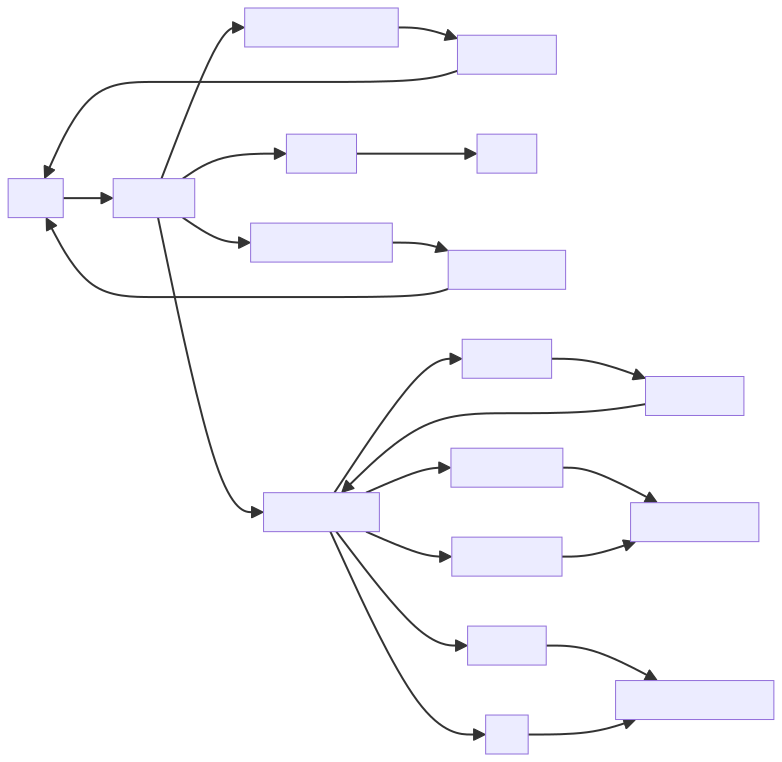
\includegraphics[keepaspectratio,alt={Diagram of RFC status}]{rfc-diagram.png}}
\caption{Diagram of RFC status}
\end{figure}

When reading an RFC, you might notice an error, or have comments or
suggestions. It is possible to report a significant error by following
the \emph{Submit Errata} link on the info page. If you have technical
comments or suggestions, consider joining the relevant working group by
\href{https://www.ietf.org/participate/}{participating in the IETF} or
\href{https://www.irtf.org/}{IRTF}.

An important RFC is the latest version of
\href{https://www.rfc-editor.org/info/bcp220}{IPv6 Node Requirements},
which cites numerous other RFCs. However, at the time of this writing,
there are already at least 12 more recent IPv6 RFCs from the IETF since
the last update of the node requirements. The documents of the main IETF
working groups concerned with IPv6 are listed at the
\href{https://datatracker.ietf.org/wg/6man/documents/}{6MAN} and
\href{https://datatracker.ietf.org/wg/v6ops/documents/}{V6OPS} web
pages. Beware of the fact that these pages list unapproved drafts and
obsolete RFCs as well as current RFCs.

In a few cases in this book, we refer to unapproved drafts (usually
known as Internet-Drafts or I-Ds). Officially, it is inappropriate to
use I-Ds as reference material. While sometimes very useful and
up-to-date, such drafts do not have the same status as RFCs and should
not be relied on as stable documents
{[}\href{https://datatracker.ietf.org/doc/draft-wkumari-not-a-draft/}{draft-wkumari-not-a-draft}{]}.
They have not been thoroughly reviewed, they may be wrong, and there is
a high probability that they will never be published as an RFC. A draft
whose file name starts "draft-ietf-" has been adopted by an IETF working
group, so it has passed a preliminary review, but it is still a draft,
it may still be wrong, and may never become an RFC.

Drafts whose names do \emph{not} start "draft-ietf-" are named according
to an agreed
\href{https://authors.ietf.org/naming-your-internet-draft}{convention},
but they have almostly certainly not been adopted by an IETF working
group and should be read with caution. The definitive source of
information about I-Ds is the \href{https://datatracker.ietf.org/}{IETF
data tracker}.

All I-Ds are open to comment and contain contact information. Feel free
to email their authors or the relevant mailing list. This diagram gives
an overview:

\begin{figure}
\centering
\pandocbounded{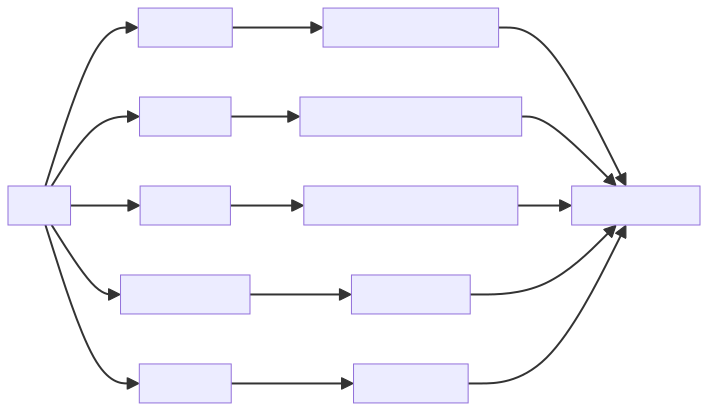
\includegraphics[keepaspectratio,alt={Diagram of I-D status}]{id-diagram.png}}
\caption{Diagram of I-D status}
\end{figure}

There are also numerous books, book chapters, and other documents about
IPv6. However, any source that is more than one or two years old is
likely to be out of date in some aspects, and discuss obsolete
deployment options. Here are some starting points:

\begin{itemize}
\item
  \href{https://docs.google.com/document/d/1WohukYWdlFcEaSm-SQtX5Zgrkr-FZiZnfhlvoFi5Bl0/edit}{Inessential
  IPv6}. This project overlaps in intent with book6 so we will attempt
  to coordinate.
\item
  \href{https://repository.jisc.ac.uk/8349/1/janet-ipv6-technical-guide.pdf}{The
  JANET technical guide to IPv6} (2021)
\item
  \href{https://academy.apnic.net/en/course/ipv6-fundamentals}{The APNIC
  IPv6 Fundamentals Course}
\item
  The RIPE NCC \emph{Advanced IPv6} training course. Everyone can
  download their excellent 264 slides, which cover very many topics:
  \href{https://www.ripe.net/documents/3822/AdvancedIPv6-Slides_xDUF4U9.pdf}{download
  37MB}.
\item
  Olivier Bonaventure\textquotesingle s
  \href{https://beta.computer-networking.info/syllabus/default/protocols/ipv6.html\#ip-version-6}{Computer
  Networking : Principles, Protocols and Practice} (2019)
\item
  ISOC\textquotesingle s
  \href{https://www.internetsociety.org/resources/deploy360/ipv6/security/ipv4-engineers/}{IPv6
  Security for IPv4 Engineers} (2019)
\item
  ISOC\textquotesingle s
  \href{https://www.internetsociety.org/deploy360/ipv6/security/faq/}{IPv6
  Security FAQ} (2019)
\item
  Graziani, Rick. IPv6 Fundamentals: A Straightforward Approach to
  Understanding IPv6 (2nd edition), Cisco Press, ISBN 978-1587144776
  (2017). A very good book, but years\textquotesingle{} worth of
  progress has happened since then!
\item
  Great IPv6 blogging from \href{https://ipv6.iljitsch.com/}{Iljitsch
  van Beijnum}
\item
  van Beijnum, Iljitsch.
  \href{https://www.iljitsch.com/2022/11-18-new-e-book-internet-routing-with-bgp.html}{Internet
  Routing with BGP} (2022). This contains a lot about IPv6 inter-domain
  routing.
\item
  more suggestions welcome!
\end{itemize}

\hyperref[rfc-bibliography]{RFC bibliography}

\subsubsection{\texorpdfstring{\hyperref[list-of-contents]{Back to main
Contents}}{Back to main Contents}}\label{back-to-main-contents-10}

\pagebreak

\subsection{RFC bibliography}\label{rfc-bibliography}

This section is a machine-generated list of all current RFCs that
mention IPv6 or DHCPv6 in their title or come from the major IPv6
working groups. Obsolete RFCs are not included. There are subsections
for Standards, BCPs, Informational and Experimental RFCs. Be
\emph{cautious} about old Informational or Experimental RFCs - they may
be misleading as well as out of date. Also see
\hyperref[obsolete-features-in-ipv6]{10. Obsolete Features in IPv6}.

RFCbib6 run at 2026-02-12 15:56:16 UTC+1300 (504 RFCs found)

\subsubsection{Standards Track (271
RFCs)}\label{standards-track-271-rfcs}

\begin{itemize}
\tightlist
\item
  \href{https://www.rfc-editor.org/info/rfc2080}{RFC 2080}: RIPng for
  IPv6
\item
  \href{https://www.rfc-editor.org/info/rfc2428}{RFC 2428}: FTP
  Extensions for IPv6 and NATs
\item
  \href{https://www.rfc-editor.org/info/rfc2464}{RFC 2464}: Transmission
  of IPv6 Packets over Ethernet Networks
\item
  \href{https://www.rfc-editor.org/info/rfc2467}{RFC 2467}: Transmission
  of IPv6 Packets over FDDI Networks
\item
  \href{https://www.rfc-editor.org/info/rfc2470}{RFC 2470}: Transmission
  of IPv6 Packets over Token Ring Networks
\item
  \href{https://www.rfc-editor.org/info/rfc2473}{RFC 2473}: Generic
  Packet Tunneling in IPv6 Specification
\item
  \href{https://www.rfc-editor.org/info/rfc2474}{RFC 2474}: Definition
  of the Differentiated Services Field (DS Field) in the IPv4 and IPv6
  Headers
\item
  \href{https://www.rfc-editor.org/info/rfc2491}{RFC 2491}: IPv6 over
  Non-Broadcast Multiple Access (NBMA) networks
\item
  \href{https://www.rfc-editor.org/info/rfc2492}{RFC 2492}: IPv6 over
  ATM Networks
\item
  \href{https://www.rfc-editor.org/info/rfc2497}{RFC 2497}: Transmission
  of IPv6 Packets over ARCnet Networks
\item
  \href{https://www.rfc-editor.org/info/rfc2526}{RFC 2526}: Reserved
  IPv6 Subnet Anycast Addresses
\item
  \href{https://www.rfc-editor.org/info/rfc2529}{RFC 2529}: Transmission
  of IPv6 over IPv4 Domains without Explicit Tunnels
\item
  \href{https://www.rfc-editor.org/info/rfc2545}{RFC 2545}: Use of BGP-4
  Multiprotocol Extensions for IPv6 Inter-Domain Routing
\item
  \href{https://www.rfc-editor.org/info/rfc2590}{RFC 2590}: Transmission
  of IPv6 Packets over Frame Relay Networks Specification
\item
  \href{https://www.rfc-editor.org/info/rfc2675}{RFC 2675}: IPv6
  Jumbograms
\item
  \href{https://www.rfc-editor.org/info/rfc2710}{RFC 2710}: Multicast
  Listener Discovery (MLD) for IPv6
\item
  \href{https://www.rfc-editor.org/info/rfc2711}{RFC 2711}: IPv6 Router
  Alert Option
\item
  \href{https://www.rfc-editor.org/info/rfc2894}{RFC 2894}: Router
  Renumbering for IPv6
\item
  \href{https://www.rfc-editor.org/info/rfc3056}{RFC 3056}: Connection
  of IPv6 Domains via IPv4 Clouds
\item
  \href{https://www.rfc-editor.org/info/rfc3111}{RFC 3111}: Service
  Location Protocol Modifications for IPv6
\item
  \href{https://www.rfc-editor.org/info/rfc3122}{RFC 3122}: Extensions
  to IPv6 Neighbor Discovery for Inverse Discovery Specification
\item
  \href{https://www.rfc-editor.org/info/rfc3146}{RFC 3146}: Transmission
  of IPv6 Packets over IEEE 1394 Networks
\item
  \href{https://www.rfc-editor.org/info/rfc3162}{RFC 3162}: RADIUS and
  IPv6
\item
  \href{https://www.rfc-editor.org/info/rfc3175}{RFC 3175}: Aggregation
  of RSVP for IPv4 and IPv6 Reservations
\item
  \href{https://www.rfc-editor.org/info/rfc3226}{RFC 3226}: DNSSEC and
  IPv6 A6 aware server/resolver message size requirements
\item
  \href{https://www.rfc-editor.org/info/rfc3306}{RFC 3306}:
  Unicast-Prefix-based IPv6 Multicast Addresses
\item
  \href{https://www.rfc-editor.org/info/rfc3307}{RFC 3307}: Allocation
  Guidelines for IPv6 Multicast Addresses
\item
  \href{https://www.rfc-editor.org/info/rfc3319}{RFC 3319}: Dynamic Host
  Configuration Protocol (DHCPv6) Options for Session Initiation
  Protocol (SIP) Servers
\item
  \href{https://www.rfc-editor.org/info/rfc3595}{RFC 3595}: Textual
  Conventions for IPv6 Flow Label
\item
  \href{https://www.rfc-editor.org/info/rfc3596}{RFC 3596}
  (\href{https://www.rfc-editor.org/info/std88}{STD 88}): DNS Extensions
  to Support IP Version 6
\item
  \href{https://www.rfc-editor.org/info/rfc3646}{RFC 3646}: DNS
  Configuration options for Dynamic Host Configuration Protocol for IPv6
  (DHCPv6)
\item
  \href{https://www.rfc-editor.org/info/rfc3776}{RFC 3776}: Using IPsec
  to Protect Mobile IPv6 Signaling Between Mobile Nodes and Home Agents
\item
  \href{https://www.rfc-editor.org/info/rfc3898}{RFC 3898}: Network
  Information Service (NIS) Configuration Options for Dynamic Host
  Configuration Protocol for IPv6 (DHCPv6)
\item
  \href{https://www.rfc-editor.org/info/rfc3956}{RFC 3956}: Embedding
  the Rendezvous Point (RP) Address in an IPv6 Multicast Address
\item
  \href{https://www.rfc-editor.org/info/rfc4007}{RFC 4007}: IPv6 Scoped
  Address Architecture
\item
  \href{https://www.rfc-editor.org/info/rfc4075}{RFC 4075}: Simple
  Network Time Protocol (SNTP) Configuration Option for DHCPv6
\item
  \href{https://www.rfc-editor.org/info/rfc4193}{RFC 4193}: Unique Local
  IPv6 Unicast Addresses
\item
  \href{https://www.rfc-editor.org/info/rfc4213}{RFC 4213}: Basic
  Transition Mechanisms for IPv6 Hosts and Routers
\item
  \href{https://www.rfc-editor.org/info/rfc4283}{RFC 4283}: Mobile Node
  Identifier Option for Mobile IPv6 (MIPv6)
\item
  \href{https://www.rfc-editor.org/info/rfc4291}{RFC 4291}: IP Version 6
  Addressing Architecture
\item
  \href{https://www.rfc-editor.org/info/rfc4295}{RFC 4295}: Mobile IPv6
  Management Information Base
\item
  \href{https://www.rfc-editor.org/info/rfc4311}{RFC 4311}: IPv6
  Host-to-Router Load Sharing
\item
  \href{https://www.rfc-editor.org/info/rfc4338}{RFC 4338}: Transmission
  of IPv6, IPv4, and Address Resolution Protocol (ARP) Packets over
  Fibre Channel
\item
  \href{https://www.rfc-editor.org/info/rfc4380}{RFC 4380}: Teredo:
  Tunneling IPv6 over UDP through Network Address Translations (NATs)
\item
  \href{https://www.rfc-editor.org/info/rfc4429}{RFC 4429}: Optimistic
  Duplicate Address Detection (DAD) for IPv6
\item
  \href{https://www.rfc-editor.org/info/rfc4443}{RFC 4443}
  (\href{https://www.rfc-editor.org/info/std89}{STD 89}): Internet
  Control Message Protocol (ICMPv6) for the Internet Protocol Version 6
  (IPv6) Specification
\item
  \href{https://www.rfc-editor.org/info/rfc4449}{RFC 4449}: Securing
  Mobile IPv6 Route Optimization Using a Static Shared Key
\item
  \href{https://www.rfc-editor.org/info/rfc4489}{RFC 4489}: A Method for
  Generating Link-Scoped IPv6 Multicast Addresses
\item
  \href{https://www.rfc-editor.org/info/rfc4580}{RFC 4580}: Dynamic Host
  Configuration Protocol for IPv6 (DHCPv6) Relay Agent Subscriber-ID
  Option
\item
  \href{https://www.rfc-editor.org/info/rfc4649}{RFC 4649}: Dynamic Host
  Configuration Protocol for IPv6 (DHCPv6) Relay Agent Remote-ID Option
\item
  \href{https://www.rfc-editor.org/info/rfc4659}{RFC 4659}: BGP-MPLS IP
  Virtual Private Network (VPN) Extension for IPv6 VPN
\item
  \href{https://www.rfc-editor.org/info/rfc4668}{RFC 4668}: RADIUS
  Authentication Client MIB for IPv6
\item
  \href{https://www.rfc-editor.org/info/rfc4669}{RFC 4669}: RADIUS
  Authentication Server MIB for IPv6
\item
  \href{https://www.rfc-editor.org/info/rfc4704}{RFC 4704}: The Dynamic
  Host Configuration Protocol for IPv6 (DHCPv6) Client Fully Qualified
  Domain Name (FQDN) Option
\item
  \href{https://www.rfc-editor.org/info/rfc4727}{RFC 4727}: Experimental
  Values In IPv4, IPv6, ICMPv4, ICMPv6, UDP, and TCP Headers
\item
  \href{https://www.rfc-editor.org/info/rfc4776}{RFC 4776}: Dynamic Host
  Configuration Protocol (DHCPv4 and DHCPv6) Option for Civic Addresses
  Configuration Information
\item
  \href{https://www.rfc-editor.org/info/rfc4798}{RFC 4798}: Connecting
  IPv6 Islands over IPv4 MPLS Using IPv6 Provider Edge Routers (6PE)
\item
  \href{https://www.rfc-editor.org/info/rfc4818}{RFC 4818}: RADIUS
  Delegated-IPv6-Prefix Attribute
\item
  \href{https://www.rfc-editor.org/info/rfc4861}{RFC 4861}: Neighbor
  Discovery for IP version 6 (IPv6)
\item
  \href{https://www.rfc-editor.org/info/rfc4862}{RFC 4862}: IPv6
  Stateless Address Autoconfiguration
\item
  \href{https://www.rfc-editor.org/info/rfc4866}{RFC 4866}: Enhanced
  Route Optimization for Mobile IPv6
\item
  \href{https://www.rfc-editor.org/info/rfc4877}{RFC 4877}: Mobile IPv6
  Operation with IKEv2 and the Revised IPsec Architecture
\item
  \href{https://www.rfc-editor.org/info/rfc4944}{RFC 4944}: Transmission
  of IPv6 Packets over IEEE 802.15.4 Networks
\item
  \href{https://www.rfc-editor.org/info/rfc4994}{RFC 4994}: DHCPv6 Relay
  Agent Echo Request Option
\item
  \href{https://www.rfc-editor.org/info/rfc5007}{RFC 5007}: DHCPv6
  Leasequery
\item
  \href{https://www.rfc-editor.org/info/rfc5026}{RFC 5026}: Mobile IPv6
  Bootstrapping in Split Scenario
\item
  \href{https://www.rfc-editor.org/info/rfc5072}{RFC 5072}: IP Version 6
  over PPP
\item
  \href{https://www.rfc-editor.org/info/rfc5094}{RFC 5094}: Mobile IPv6
  Vendor Specific Option
\item
  \href{https://www.rfc-editor.org/info/rfc5095}{RFC 5095}: Deprecation
  of Type 0 Routing Headers in IPv6
\item
  \href{https://www.rfc-editor.org/info/rfc5096}{RFC 5096}: Mobile IPv6
  Experimental Messages
\item
  \href{https://www.rfc-editor.org/info/rfc5121}{RFC 5121}: Transmission
  of IPv6 via the IPv6 Convergence Sublayer over IEEE 802.16 Networks
\item
  \href{https://www.rfc-editor.org/info/rfc5172}{RFC 5172}: Negotiation
  for IPv6 Datagram Compression Using IPv6 Control Protocol
\item
  \href{https://www.rfc-editor.org/info/rfc5175}{RFC 5175}: IPv6 Router
  Advertisement Flags Option
\item
  \href{https://www.rfc-editor.org/info/rfc5213}{RFC 5213}: Proxy Mobile
  IPv6
\item
  \href{https://www.rfc-editor.org/info/rfc5269}{RFC 5269}: Distributing
  a Symmetric Fast Mobile IPv6 (FMIPv6) Handover Key Using SEcure
  Neighbor Discovery (SEND)
\item
  \href{https://www.rfc-editor.org/info/rfc5308}{RFC 5308}: Routing IPv6
  with IS-IS
\item
  \href{https://www.rfc-editor.org/info/rfc5340}{RFC 5340}: OSPF for
  IPv6
\item
  \href{https://www.rfc-editor.org/info/rfc5350}{RFC 5350}: IANA
  Considerations for the IPv4 and IPv6 Router Alert Options
\item
  \href{https://www.rfc-editor.org/info/rfc5380}{RFC 5380}: Hierarchical
  Mobile IPv6 (HMIPv6) Mobility Management
\item
  \href{https://www.rfc-editor.org/info/rfc5447}{RFC 5447}: Diameter
  Mobile IPv6: Support for Network Access Server to Diameter Server
  Interaction
\item
  \href{https://www.rfc-editor.org/info/rfc5453}{RFC 5453}: Reserved
  IPv6 Interface Identifiers
\item
  \href{https://www.rfc-editor.org/info/rfc5460}{RFC 5460}: DHCPv6 Bulk
  Leasequery
\item
  \href{https://www.rfc-editor.org/info/rfc5533}{RFC 5533}: Shim6: Level
  3 Multihoming Shim Protocol for IPv6
\item
  \href{https://www.rfc-editor.org/info/rfc5534}{RFC 5534}: Failure
  Detection and Locator Pair Exploration Protocol for IPv6 Multihoming
\item
  \href{https://www.rfc-editor.org/info/rfc5555}{RFC 5555}: Mobile IPv6
  Support for Dual Stack Hosts and Routers
\item
  \href{https://www.rfc-editor.org/info/rfc5568}{RFC 5568}: Mobile IPv6
  Fast Handovers
\item
  \href{https://www.rfc-editor.org/info/rfc5678}{RFC 5678}: Dynamic Host
  Configuration Protocol (DHCPv4 and DHCPv6) Options for IEEE 802.21
  Mobility Services (MoS) Discovery
\item
  \href{https://www.rfc-editor.org/info/rfc5701}{RFC 5701}: IPv6 Address
  Specific BGP Extended Community Attribute
\item
  \href{https://www.rfc-editor.org/info/rfc5722}{RFC 5722}: Handling of
  Overlapping IPv6 Fragments
\item
  \href{https://www.rfc-editor.org/info/rfc5778}{RFC 5778}: Diameter
  Mobile IPv6: Support for Home Agent to Diameter Server Interaction
\item
  \href{https://www.rfc-editor.org/info/rfc5779}{RFC 5779}: Diameter
  Proxy Mobile IPv6: Mobile Access Gateway and Local Mobility Anchor
  Interaction with Diameter Server
\item
  \href{https://www.rfc-editor.org/info/rfc5844}{RFC 5844}: IPv4 Support
  for Proxy Mobile IPv6
\item
  \href{https://www.rfc-editor.org/info/rfc5845}{RFC 5845}: Generic
  Routing Encapsulation (GRE) Key Option for Proxy Mobile IPv6
\item
  \href{https://www.rfc-editor.org/info/rfc5846}{RFC 5846}: Binding
  Revocation for IPv6 Mobility
\item
  \href{https://www.rfc-editor.org/info/rfc5847}{RFC 5847}: Heartbeat
  Mechanism for Proxy Mobile IPv6
\item
  \href{https://www.rfc-editor.org/info/rfc5871}{RFC 5871}: IANA
  Allocation Guidelines for the IPv6 Routing Header
\item
  \href{https://www.rfc-editor.org/info/rfc5881}{RFC 5881}:
  Bidirectional Forwarding Detection (BFD) for IPv4 and IPv6 (Single
  Hop)
\item
  \href{https://www.rfc-editor.org/info/rfc5908}{RFC 5908}: Network Time
  Protocol (NTP) Server Option for DHCPv6
\item
  \href{https://www.rfc-editor.org/info/rfc5942}{RFC 5942}: IPv6 Subnet
  Model: The Relationship between Links and Subnet Prefixes
\item
  \href{https://www.rfc-editor.org/info/rfc5949}{RFC 5949}: Fast
  Handovers for Proxy Mobile IPv6
\item
  \href{https://www.rfc-editor.org/info/rfc5952}{RFC 5952}: A
  Recommendation for IPv6 Address Text Representation
\item
  \href{https://www.rfc-editor.org/info/rfc5954}{RFC 5954}: Essential
  Correction for IPv6 ABNF and URI Comparison in RFC 3261
\item
  \href{https://www.rfc-editor.org/info/rfc5969}{RFC 5969}: IPv6 Rapid
  Deployment on IPv4 Infrastructures (6rd) -\/- Protocol Specification
\item
  \href{https://www.rfc-editor.org/info/rfc5970}{RFC 5970}: DHCPv6
  Options for Network Boot
\item
  \href{https://www.rfc-editor.org/info/rfc6052}{RFC 6052}: IPv6
  Addressing of IPv4/IPv6 Translators
\item
  \href{https://www.rfc-editor.org/info/rfc6059}{RFC 6059}: Simple
  Procedures for Detecting Network Attachment in IPv6
\item
  \href{https://www.rfc-editor.org/info/rfc6085}{RFC 6085}: Address
  Mapping of IPv6 Multicast Packets on Ethernet
\item
  \href{https://www.rfc-editor.org/info/rfc6089}{RFC 6089}: Flow
  Bindings in Mobile IPv6 and Network Mobility (NEMO) Basic Support
\item
  \href{https://www.rfc-editor.org/info/rfc6119}{RFC 6119}: IPv6 Traffic
  Engineering in IS-IS
\item
  \href{https://www.rfc-editor.org/info/rfc6146}{RFC 6146}: Stateful
  NAT64: Network Address and Protocol Translation from IPv6 Clients to
  IPv4 Servers
\item
  \href{https://www.rfc-editor.org/info/rfc6147}{RFC 6147}: DNS64: DNS
  Extensions for Network Address Translation from IPv6 Clients to IPv4
  Servers
\item
  \href{https://www.rfc-editor.org/info/rfc6153}{RFC 6153}: DHCPv4 and
  DHCPv6 Options for Access Network Discovery and Selection Function
  (ANDSF) Discovery
\item
  \href{https://www.rfc-editor.org/info/rfc6157}{RFC 6157}: IPv6
  Transition in the Session Initiation Protocol (SIP)
\item
  \href{https://www.rfc-editor.org/info/rfc6164}{RFC 6164}: Using
  127-Bit IPv6 Prefixes on Inter-Router Links
\item
  \href{https://www.rfc-editor.org/info/rfc6221}{RFC 6221}: Lightweight
  DHCPv6 Relay Agent
\item
  \href{https://www.rfc-editor.org/info/rfc6275}{RFC 6275}: Mobility
  Support in IPv6
\item
  \href{https://www.rfc-editor.org/info/rfc6276}{RFC 6276}: DHCPv6
  Prefix Delegation for Network Mobility (NEMO)
\item
  \href{https://www.rfc-editor.org/info/rfc6282}{RFC 6282}: Compression
  Format for IPv6 Datagrams over IEEE 802.15.4-Based Networks
\item
  \href{https://www.rfc-editor.org/info/rfc6334}{RFC 6334}: Dynamic Host
  Configuration Protocol for IPv6 (DHCPv6) Option for Dual-Stack Lite
\item
  \href{https://www.rfc-editor.org/info/rfc6355}{RFC 6355}: Definition
  of the UUID-Based DHCPv6 Unique Identifier (DUID-UUID)
\item
  \href{https://www.rfc-editor.org/info/rfc6384}{RFC 6384}: An FTP
  Application Layer Gateway (ALG) for IPv6-to-IPv4 Translation
\item
  \href{https://www.rfc-editor.org/info/rfc6437}{RFC 6437}: IPv6 Flow
  Label Specification
\item
  \href{https://www.rfc-editor.org/info/rfc6438}{RFC 6438}: Using the
  IPv6 Flow Label for Equal Cost Multipath Routing and Link Aggregation
  in Tunnels
\item
  \href{https://www.rfc-editor.org/info/rfc6440}{RFC 6440}: The EAP
  Re-authentication Protocol (ERP) Local Domain Name DHCPv6 Option
\item
  \href{https://www.rfc-editor.org/info/rfc6463}{RFC 6463}: Runtime
  Local Mobility Anchor (LMA) Assignment Support for Proxy Mobile IPv6
\item
  \href{https://www.rfc-editor.org/info/rfc6475}{RFC 6475}: Proxy Mobile
  IPv6 Management Information Base
\item
  \href{https://www.rfc-editor.org/info/rfc6515}{RFC 6515}: IPv4 and
  IPv6 Infrastructure Addresses in BGP Updates for Multicast VPN
\item
  \href{https://www.rfc-editor.org/info/rfc6516}{RFC 6516}: IPv6
  Multicast VPN (MVPN) Support Using PIM Control Plane and Selective
  Provider Multicast Service Interface (S-PMSI) Join Messages
\item
  \href{https://www.rfc-editor.org/info/rfc6543}{RFC 6543}: Reserved
  IPv6 Interface Identifier for Proxy Mobile IPv6
\item
  \href{https://www.rfc-editor.org/info/rfc6550}{RFC 6550}: RPL: IPv6
  Routing Protocol for Low-Power and Lossy Networks
\item
  \href{https://www.rfc-editor.org/info/rfc6553}{RFC 6553}: The Routing
  Protocol for Low-Power and Lossy Networks (RPL) Option for Carrying
  RPL Information in Data-Plane Datagrams
\item
  \href{https://www.rfc-editor.org/info/rfc6554}{RFC 6554}: An IPv6
  Routing Header for Source Routes with the Routing Protocol for
  Low-Power and Lossy Networks (RPL)
\item
  \href{https://www.rfc-editor.org/info/rfc6564}{RFC 6564}: A Uniform
  Format for IPv6 Extension Headers
\item
  \href{https://www.rfc-editor.org/info/rfc6572}{RFC 6572}: RADIUS
  Support for Proxy Mobile IPv6
\item
  \href{https://www.rfc-editor.org/info/rfc6602}{RFC 6602}: Bulk Binding
  Update Support for Proxy Mobile IPv6
\item
  \href{https://www.rfc-editor.org/info/rfc6603}{RFC 6603}: Prefix
  Exclude Option for DHCPv6-based Prefix Delegation
\item
  \href{https://www.rfc-editor.org/info/rfc6607}{RFC 6607}: Virtual
  Subnet Selection Options for DHCPv4 and DHCPv6
\item
  \href{https://www.rfc-editor.org/info/rfc6610}{RFC 6610}: DHCP Options
  for Home Information Discovery in Mobile IPv6 (MIPv6)
\item
  \href{https://www.rfc-editor.org/info/rfc6611}{RFC 6611}: Mobile IPv6
  (MIPv6) Bootstrapping for the Integrated Scenario
\item
  \href{https://www.rfc-editor.org/info/rfc6620}{RFC 6620}: FCFS SAVI:
  First-Come, First-Served Source Address Validation Improvement for
  Locally Assigned IPv6 Addresses
\item
  \href{https://www.rfc-editor.org/info/rfc6644}{RFC 6644}: Rebind
  Capability in DHCPv6 Reconfigure Messages
\item
  \href{https://www.rfc-editor.org/info/rfc6705}{RFC 6705}: Localized
  Routing for Proxy Mobile IPv6
\item
  \href{https://www.rfc-editor.org/info/rfc6724}{RFC 6724}: Default
  Address Selection for Internet Protocol Version 6 (IPv6)
\item
  \href{https://www.rfc-editor.org/info/rfc6757}{RFC 6757}: Access
  Network Identifier (ANI) Option for Proxy Mobile IPv6
\item
  \href{https://www.rfc-editor.org/info/rfc6775}{RFC 6775}: Neighbor
  Discovery Optimization for IPv6 over Low-Power Wireless Personal Area
  Networks (6LoWPANs)
\item
  \href{https://www.rfc-editor.org/info/rfc6784}{RFC 6784}: Kerberos
  Options for DHCPv6
\item
  \href{https://www.rfc-editor.org/info/rfc6788}{RFC 6788}: The
  Line-Identification Option
\item
  \href{https://www.rfc-editor.org/info/rfc6791}{RFC 6791}: Stateless
  Source Address Mapping for ICMPv6 Packets
\item
  \href{https://www.rfc-editor.org/info/rfc6909}{RFC 6909}: IPv4 Traffic
  Offload Selector Option for Proxy Mobile IPv6
\item
  \href{https://www.rfc-editor.org/info/rfc6911}{RFC 6911}: RADIUS
  Attributes for IPv6 Access Networks
\item
  \href{https://www.rfc-editor.org/info/rfc6930}{RFC 6930}: RADIUS
  Attribute for IPv6 Rapid Deployment on IPv4 Infrastructures (6rd)
\item
  \href{https://www.rfc-editor.org/info/rfc6935}{RFC 6935}: IPv6 and UDP
  Checksums for Tunneled Packets
\item
  \href{https://www.rfc-editor.org/info/rfc6936}{RFC 6936}:
  Applicability Statement for the Use of IPv6 UDP Datagrams with Zero
  Checksums
\item
  \href{https://www.rfc-editor.org/info/rfc6939}{RFC 6939}: Client
  Link-Layer Address Option in DHCPv6
\item
  \href{https://www.rfc-editor.org/info/rfc6946}{RFC 6946}: Processing
  of IPv6 "Atomic" Fragments
\item
  \href{https://www.rfc-editor.org/info/rfc6957}{RFC 6957}: Duplicate
  Address Detection Proxy
\item
  \href{https://www.rfc-editor.org/info/rfc6977}{RFC 6977}: Triggering
  DHCPv6 Reconfiguration from Relay Agents
\item
  \href{https://www.rfc-editor.org/info/rfc6980}{RFC 6980}: Security
  Implications of IPv6 Fragmentation with IPv6 Neighbor Discovery
\item
  \href{https://www.rfc-editor.org/info/rfc7037}{RFC 7037}: RADIUS
  Option for the DHCPv6 Relay Agent
\item
  \href{https://www.rfc-editor.org/info/rfc7045}{RFC 7045}: Transmission
  and Processing of IPv6 Extension Headers
\item
  \href{https://www.rfc-editor.org/info/rfc7048}{RFC 7048}: Neighbor
  Unreachability Detection Is Too Impatient
\item
  \href{https://www.rfc-editor.org/info/rfc7050}{RFC 7050}: Discovery of
  the IPv6 Prefix Used for IPv6 Address Synthesis
\item
  \href{https://www.rfc-editor.org/info/rfc7077}{RFC 7077}: Update
  Notifications for Proxy Mobile IPv6
\item
  \href{https://www.rfc-editor.org/info/rfc7078}{RFC 7078}: Distributing
  Address Selection Policy Using DHCPv6
\item
  \href{https://www.rfc-editor.org/info/rfc7112}{RFC 7112}: Implications
  of Oversized IPv6 Header Chains
\item
  \href{https://www.rfc-editor.org/info/rfc7136}{RFC 7136}: Significance
  of IPv6 Interface Identifiers
\item
  \href{https://www.rfc-editor.org/info/rfc7148}{RFC 7148}: Prefix
  Delegation Support for Proxy Mobile IPv6
\item
  \href{https://www.rfc-editor.org/info/rfc7156}{RFC 7156}: Diameter
  Support for Proxy Mobile IPv6 Localized Routing
\item
  \href{https://www.rfc-editor.org/info/rfc7217}{RFC 7217}: A Method for
  Generating Semantically Opaque Interface Identifiers with IPv6
  Stateless Address Autoconfiguration (SLAAC)
\item
  \href{https://www.rfc-editor.org/info/rfc7222}{RFC 7222}:
  Quality-of-Service Option for Proxy Mobile IPv6
\item
  \href{https://www.rfc-editor.org/info/rfc7225}{RFC 7225}: Discovering
  NAT64 IPv6 Prefixes Using the Port Control Protocol (PCP)
\item
  \href{https://www.rfc-editor.org/info/rfc7335}{RFC 7335}: IPv4 Service
  Continuity Prefix
\item
  \href{https://www.rfc-editor.org/info/rfc7341}{RFC 7341}:
  DHCPv4-over-DHCPv6 (DHCP 4o6) Transport
\item
  \href{https://www.rfc-editor.org/info/rfc7343}{RFC 7343}: An IPv6
  Prefix for Overlay Routable Cryptographic Hash Identifiers Version 2
  (ORCHIDv2)
\item
  \href{https://www.rfc-editor.org/info/rfc7346}{RFC 7346}: IPv6
  Multicast Address Scopes
\item
  \href{https://www.rfc-editor.org/info/rfc7371}{RFC 7371}: Updates to
  the IPv6 Multicast Addressing Architecture
\item
  \href{https://www.rfc-editor.org/info/rfc7388}{RFC 7388}: Definition
  of Managed Objects for IPv6 over Low-Power Wireless Personal Area
  Networks (6LoWPANs)
\item
  \href{https://www.rfc-editor.org/info/rfc7389}{RFC 7389}: Separation
  of Control and User Plane for Proxy Mobile IPv6
\item
  \href{https://www.rfc-editor.org/info/rfc7400}{RFC 7400}: 6LoWPAN-GHC:
  Generic Header Compression for IPv6 over Low-Power Wireless Personal
  Area Networks (6LoWPANs)
\item
  \href{https://www.rfc-editor.org/info/rfc7428}{RFC 7428}: Transmission
  of IPv6 Packets over ITU-T G.9959 Networks
\item
  \href{https://www.rfc-editor.org/info/rfc7527}{RFC 7527}: Enhanced
  Duplicate Address Detection
\item
  \href{https://www.rfc-editor.org/info/rfc7552}{RFC 7552}: Updates to
  LDP for IPv6
\item
  \href{https://www.rfc-editor.org/info/rfc7559}{RFC 7559}: Packet-Loss
  Resiliency for Router Solicitations
\item
  \href{https://www.rfc-editor.org/info/rfc7563}{RFC 7563}: Extensions
  to the Proxy Mobile IPv6 (PMIPv6) Access Network Identifier Option
\item
  \href{https://www.rfc-editor.org/info/rfc7598}{RFC 7598}: DHCPv6
  Options for Configuration of Softwire Address and Port-Mapped Clients
\item
  \href{https://www.rfc-editor.org/info/rfc7653}{RFC 7653}: DHCPv6
  Active Leasequery
\item
  \href{https://www.rfc-editor.org/info/rfc7668}{RFC 7668}: IPv6 over
  BLUETOOTH(R) Low Energy
\item
  \href{https://www.rfc-editor.org/info/rfc7676}{RFC 7676}: IPv6 Support
  for Generic Routing Encapsulation (GRE)
\item
  \href{https://www.rfc-editor.org/info/rfc7678}{RFC 7678}:
  Attribute-Value Pairs for Provisioning Customer Equipment Supporting
  IPv4-Over-IPv6 Transitional Solutions
\item
  \href{https://www.rfc-editor.org/info/rfc7755}{RFC 7755}: SIIT-DC:
  Stateless IP/ICMP Translation for IPv6 Data Center Environments
\item
  \href{https://www.rfc-editor.org/info/rfc7756}{RFC 7756}: Stateless
  IP/ICMP Translation for IPv6 Internet Data Center Environments
  (SIIT-DC): Dual Translation Mode
\item
  \href{https://www.rfc-editor.org/info/rfc7757}{RFC 7757}
  (\href{https://www.rfc-editor.org/info/std103}{STD 103}): Explicit
  Address Mappings for Stateless IP/ICMP Translation
\item
  \href{https://www.rfc-editor.org/info/rfc7774}{RFC 7774}: Multicast
  Protocol for Low-Power and Lossy Networks (MPL) Parameter
  Configuration Option for DHCPv6
\item
  \href{https://www.rfc-editor.org/info/rfc7775}{RFC 7775}: IS-IS Route
  Preference for Extended IP and IPv6 Reachability
\item
  \href{https://www.rfc-editor.org/info/rfc7794}{RFC 7794}: IS-IS Prefix
  Attributes for Extended IPv4 and IPv6 Reachability
\item
  \href{https://www.rfc-editor.org/info/rfc7864}{RFC 7864}: Proxy Mobile
  IPv6 Extensions to Support Flow Mobility
\item
  \href{https://www.rfc-editor.org/info/rfc7881}{RFC 7881}: Seamless
  Bidirectional Forwarding Detection (S-BFD) for IPv4, IPv6, and MPLS
\item
  \href{https://www.rfc-editor.org/info/rfc7949}{RFC 7949}: OSPFv3 over
  IPv4 for IPv6 Transition
\item
  \href{https://www.rfc-editor.org/info/rfc8025}{RFC 8025}: IPv6 over
  Low-Power Wireless Personal Area Network (6LoWPAN) Paging Dispatch
\item
  \href{https://www.rfc-editor.org/info/rfc8026}{RFC 8026}: Unified
  IPv4-in-IPv6 Softwire Customer Premises Equipment (CPE): A
  DHCPv6-Based Prioritization Mechanism
\item
  \href{https://www.rfc-editor.org/info/rfc8028}{RFC 8028}: First-Hop
  Router Selection by Hosts in a Multi-Prefix Network
\item
  \href{https://www.rfc-editor.org/info/rfc8064}{RFC 8064}:
  Recommendation on Stable IPv6 Interface Identifiers
\item
  \href{https://www.rfc-editor.org/info/rfc8066}{RFC 8066}: IPv6 over
  Low-Power Wireless Personal Area Network (6LoWPAN) ESC Dispatch Code
  Points and Guidelines
\item
  \href{https://www.rfc-editor.org/info/rfc8105}{RFC 8105}: Transmission
  of IPv6 Packets over Digital Enhanced Cordless Telecommunications
  (DECT) Ultra Low Energy (ULE)
\item
  \href{https://www.rfc-editor.org/info/rfc8106}{RFC 8106}: IPv6 Router
  Advertisement Options for DNS Configuration
\item
  \href{https://www.rfc-editor.org/info/rfc8114}{RFC 8114}: Delivery of
  IPv4 Multicast Services to IPv4 Clients over an IPv6 Multicast Network
\item
  \href{https://www.rfc-editor.org/info/rfc8115}{RFC 8115}: DHCPv6
  Option for IPv4-Embedded Multicast and Unicast IPv6 Prefixes
\item
  \href{https://www.rfc-editor.org/info/rfc8138}{RFC 8138}: IPv6 over
  Low-Power Wireless Personal Area Network (6LoWPAN) Routing Header
\item
  \href{https://www.rfc-editor.org/info/rfc8156}{RFC 8156}: DHCPv6
  Failover Protocol
\item
  \href{https://www.rfc-editor.org/info/rfc8159}{RFC 8159}: Keyed IPv6
  Tunnel
\item
  \href{https://www.rfc-editor.org/info/rfc8163}{RFC 8163}: Transmission
  of IPv6 over Master-Slave/Token-Passing (MS/TP) Networks
\item
  \href{https://www.rfc-editor.org/info/rfc8168}{RFC 8168}: DHCPv6
  Prefix-Length Hint Issues
\item
  \href{https://www.rfc-editor.org/info/rfc8191}{RFC 8191}: Home Network
  Prefix Renumbering in Proxy Mobile IPv6 (PMIPv6)
\item
  \href{https://www.rfc-editor.org/info/rfc8200}{RFC 8200}
  (\href{https://www.rfc-editor.org/info/std86}{STD 86}): Internet
  Protocol, Version 6 (IPv6) Specification
\item
  \href{https://www.rfc-editor.org/info/rfc8201}{RFC 8201}
  (\href{https://www.rfc-editor.org/info/std87}{STD 87}): Path MTU
  Discovery for IP version 6
\item
  \href{https://www.rfc-editor.org/info/rfc8215}{RFC 8215}: Local-Use
  IPv4/IPv6 Translation Prefix
\item
  \href{https://www.rfc-editor.org/info/rfc8250}{RFC 8250}: IPv6
  Performance and Diagnostic Metrics (PDM) Destination Option
\item
  \href{https://www.rfc-editor.org/info/rfc8305}{RFC 8305}: Happy
  Eyeballs Version 2: Better Connectivity Using Concurrency
\item
  \href{https://www.rfc-editor.org/info/rfc8319}{RFC 8319}: Support for
  Adjustable Maximum Router Lifetimes per Link
\item
  \href{https://www.rfc-editor.org/info/rfc8371}{RFC 8371}: Mobile Node
  Identifier Types for MIPv6
\item
  \href{https://www.rfc-editor.org/info/rfc8425}{RFC 8425}: IANA
  Considerations for IPv6 Neighbor Discovery Prefix Information Option
  Flags
\item
  \href{https://www.rfc-editor.org/info/rfc8505}{RFC 8505}: Registration
  Extensions for IPv6 over Low-Power Wireless Personal Area Network
  (6LoWPAN) Neighbor Discovery
\item
  \href{https://www.rfc-editor.org/info/rfc8539}{RFC 8539}: Softwire
  Provisioning Using DHCPv4 over DHCPv6
\item
  \href{https://www.rfc-editor.org/info/rfc8638}{RFC 8638}: IPv4
  Multicast over an IPv6 Multicast in Softwire Mesh Networks
\item
  \href{https://www.rfc-editor.org/info/rfc8676}{RFC 8676}: YANG Modules
  for IPv4-in-IPv6 Address plus Port (A+P) Softwires
\item
  \href{https://www.rfc-editor.org/info/rfc8691}{RFC 8691}: Basic
  Support for IPv6 Networks Operating Outside the Context of a Basic
  Service Set over IEEE Std 802.11
\item
  \href{https://www.rfc-editor.org/info/rfc8754}{RFC 8754}: IPv6 Segment
  Routing Header (SRH)
\item
  \href{https://www.rfc-editor.org/info/rfc8781}{RFC 8781}: Discovering
  PREF64 in Router Advertisements
\item
  \href{https://www.rfc-editor.org/info/rfc8883}{RFC 8883}: ICMPv6
  Errors for Discarding Packets Due to Processing Limits
\item
  \href{https://www.rfc-editor.org/info/rfc8925}{RFC 8925}: IPv6-Only
  Preferred Option for DHCPv4
\item
  \href{https://www.rfc-editor.org/info/rfc8929}{RFC 8929}: IPv6
  Backbone Router
\item
  \href{https://www.rfc-editor.org/info/rfc8930}{RFC 8930}: On
  Forwarding 6LoWPAN Fragments over a Multi-Hop IPv6 Network
\item
  \href{https://www.rfc-editor.org/info/rfc8931}{RFC 8931}: IPv6 over
  Low-Power Wireless Personal Area Network (6LoWPAN) Selective Fragment
  Recovery
\item
  \href{https://www.rfc-editor.org/info/rfc8947}{RFC 8947}: Link-Layer
  Address Assignment Mechanism for DHCPv6
\item
  \href{https://www.rfc-editor.org/info/rfc8948}{RFC 8948}: Structured
  Local Address Plan (SLAP) Quadrant Selection Option for DHCPv6
\item
  \href{https://www.rfc-editor.org/info/rfc8950}{RFC 8950}: Advertising
  IPv4 Network Layer Reachability Information (NLRI) with an IPv6 Next
  Hop
\item
  \href{https://www.rfc-editor.org/info/rfc8956}{RFC 8956}:
  Dissemination of Flow Specification Rules for IPv6
\item
  \href{https://www.rfc-editor.org/info/rfc8981}{RFC 8981}: Temporary
  Address Extensions for Stateless Address Autoconfiguration in IPv6
\item
  \href{https://www.rfc-editor.org/info/rfc8983}{RFC 8983}: Internet Key
  Exchange Protocol Version 2 (IKEv2) Notification Status Types for
  IPv4/IPv6 Coexistence
\item
  \href{https://www.rfc-editor.org/info/rfc8986}{RFC 8986}: Segment
  Routing over IPv6 (SRv6) Network Programming
\item
  \href{https://www.rfc-editor.org/info/rfc8987}{RFC 8987}: DHCPv6
  Prefix Delegating Relay Requirements
\item
  \href{https://www.rfc-editor.org/info/rfc9008}{RFC 9008}: Using RPI
  Option Type, Routing Header for Source Routes, and IPv6-in-IPv6
  Encapsulation in the RPL Data Plane
\item
  \href{https://www.rfc-editor.org/info/rfc9034}{RFC 9034}: Packet
  Delivery Deadline Time in the Routing Header for IPv6 over Low-Power
  Wireless Personal Area Networks (6LoWPANs)
\item
  \href{https://www.rfc-editor.org/info/rfc9131}{RFC 9131}: Gratuitous
  Neighbor Discovery: Creating Neighbor Cache Entries on First-Hop
  Routers
\item
  \href{https://www.rfc-editor.org/info/rfc9159}{RFC 9159}: IPv6 Mesh
  over BLUETOOTH(R) Low Energy Using the Internet Protocol Support
  Profile (IPSP)
\item
  \href{https://www.rfc-editor.org/info/rfc9164}{RFC 9164}: Concise
  Binary Object Representation (CBOR) Tags for IPv4 and IPv6 Addresses
  and Prefixes
\item
  \href{https://www.rfc-editor.org/info/rfc9243}{RFC 9243}: A YANG Data
  Model for DHCPv6 Configuration
\item
  \href{https://www.rfc-editor.org/info/rfc9252}{RFC 9252}: BGP Overlay
  Services Based on Segment Routing over IPv6 (SRv6)
\item
  \href{https://www.rfc-editor.org/info/rfc9259}{RFC 9259}: Operations,
  Administration, and Maintenance (OAM) in Segment Routing over IPv6
  (SRv6)
\item
  \href{https://www.rfc-editor.org/info/rfc9343}{RFC 9343}: IPv6
  Application of the Alternate-Marking Method
\item
  \href{https://www.rfc-editor.org/info/rfc9352}{RFC 9352}: IS-IS
  Extensions to Support Segment Routing over the IPv6 Data Plane
\item
  \href{https://www.rfc-editor.org/info/rfc9354}{RFC 9354}: Transmission
  of IPv6 Packets over Power Line Communication (PLC) Networks
\item
  \href{https://www.rfc-editor.org/info/rfc9428}{RFC 9428}: Transmission
  of IPv6 Packets over Near Field Communication
\item
  \href{https://www.rfc-editor.org/info/rfc9486}{RFC 9486}: IPv6 Options
  for In Situ Operations, Administration, and Maintenance (IOAM)
\item
  \href{https://www.rfc-editor.org/info/rfc9487}{RFC 9487}: Export of
  Segment Routing over IPv6 Information in IP Flow Information Export
  (IPFIX)
\item
  \href{https://www.rfc-editor.org/info/rfc9513}{RFC 9513}: OSPFv3
  Extensions for Segment Routing over IPv6 (SRv6)
\item
  \href{https://www.rfc-editor.org/info/rfc9514}{RFC 9514}: Border
  Gateway Protocol - Link State (BGP-LS) Extensions for Segment Routing
  over IPv6 (SRv6)
\item
  \href{https://www.rfc-editor.org/info/rfc9527}{RFC 9527}: DHCPv6
  Options for the Homenet Naming Authority
\item
  \href{https://www.rfc-editor.org/info/rfc9568}{RFC 9568}: Virtual
  Router Redundancy Protocol (VRRP) Version 3 for IPv4 and IPv6
\item
  \href{https://www.rfc-editor.org/info/rfc9603}{RFC 9603}: Path
  Computation Element Communication Protocol (PCEP) Extensions for IPv6
  Segment Routing
\item
  \href{https://www.rfc-editor.org/info/rfc9673}{RFC 9673}: IPv6
  Hop-by-Hop Options Processing Procedures
\item
  \href{https://www.rfc-editor.org/info/rfc9685}{RFC 9685}: Listener
  Subscription for IPv6 Neighbor Discovery Multicast and Anycast
  Addresses
\item
  \href{https://www.rfc-editor.org/info/rfc9686}{RFC 9686}: Registering
  Self-Generated IPv6 Addresses Using DHCPv6
\item
  \href{https://www.rfc-editor.org/info/rfc9740}{RFC 9740}: New IPFIX
  Information Elements for TCP Options and IPv6 Extension Headers
\item
  \href{https://www.rfc-editor.org/info/rfc9762}{RFC 9762}: Using Router
  Advertisements to Signal the Availability of DHCPv6 Prefix Delegation
  to Clients
\item
  \href{https://www.rfc-editor.org/info/rfc9777}{RFC 9777}
  (\href{https://www.rfc-editor.org/info/std101}{STD 101}): Multicast
  Listener Discovery Version 2 (MLDv2) for IPv6
\item
  \href{https://www.rfc-editor.org/info/rfc9805}{RFC 9805}: Deprecation
  of the IPv6 Router Alert Option for New Protocols
\item
  \href{https://www.rfc-editor.org/info/rfc9819}{RFC 9819}: Argument
  Signaling for BGP Services in Segment Routing over IPv6 (SRv6)
\item
  \href{https://www.rfc-editor.org/info/rfc9844}{RFC 9844}: Entering
  IPv6 Zone Identifiers in User Interfaces
\item
  \href{https://www.rfc-editor.org/info/rfc9915}{RFC 9915}
  (\href{https://www.rfc-editor.org/info/std102}{STD 102}): Dynamic Host
  Configuration Protocol for IPv6 (DHCPv6)
\item
  \href{https://www.rfc-editor.org/info/rfc9926}{RFC 9926}: Prefix
  Registration for IPv6 Neighbor Discovery
\end{itemize}

\subsubsection{Best Current Practice (16
RFCs)}\label{best-current-practice-16-rfcs}

\begin{itemize}
\tightlist
\item
  \href{https://www.rfc-editor.org/info/rfc3901}{RFC 3901}
  (\href{https://www.rfc-editor.org/info/bcp91}{BCP 91}): DNS IPv6
  Transport Operational Guidelines
\item
  \href{https://www.rfc-editor.org/info/rfc5855}{RFC 5855}
  (\href{https://www.rfc-editor.org/info/bcp155}{BCP 155}): Nameservers
  for IPv4 and IPv6 Reverse Zones
\item
  \href{https://www.rfc-editor.org/info/rfc6177}{RFC 6177}
  (\href{https://www.rfc-editor.org/info/bcp157}{BCP 157}): IPv6 Address
  Assignment to End Sites
\item
  \href{https://www.rfc-editor.org/info/rfc6540}{RFC 6540}
  (\href{https://www.rfc-editor.org/info/bcp177}{BCP 177}): IPv6 Support
  Required for All IP-Capable Nodes
\item
  \href{https://www.rfc-editor.org/info/rfc6853}{RFC 6853}
  (\href{https://www.rfc-editor.org/info/bcp180}{BCP 180}): DHCPv6
  Redundancy Deployment Considerations
\item
  \href{https://www.rfc-editor.org/info/rfc7227}{RFC 7227}
  (\href{https://www.rfc-editor.org/info/bcp187}{BCP 187}): Guidelines
  for Creating New DHCPv6 Options
\item
  \href{https://www.rfc-editor.org/info/rfc7526}{RFC 7526}
  (\href{https://www.rfc-editor.org/info/bcp196}{BCP 196}): Deprecating
  the Anycast Prefix for 6to4 Relay Routers
\item
  \href{https://www.rfc-editor.org/info/rfc7608}{RFC 7608}
  (\href{https://www.rfc-editor.org/info/bcp198}{BCP 198}): IPv6 Prefix
  Length Recommendation for Forwarding
\item
  \href{https://www.rfc-editor.org/info/rfc7610}{RFC 7610}
  (\href{https://www.rfc-editor.org/info/bcp199}{BCP 199}):
  DHCPv6-Shield: Protecting against Rogue DHCPv6 Servers
\item
  \href{https://www.rfc-editor.org/info/rfc7772}{RFC 7772}
  (\href{https://www.rfc-editor.org/info/bcp202}{BCP 202}): Reducing
  Energy Consumption of Router Advertisements
\item
  \href{https://www.rfc-editor.org/info/rfc7934}{RFC 7934}
  (\href{https://www.rfc-editor.org/info/bcp204}{BCP 204}): Host Address
  Availability Recommendations
\item
  \href{https://www.rfc-editor.org/info/rfc8180}{RFC 8180}
  (\href{https://www.rfc-editor.org/info/bcp210}{BCP 210}): Minimal IPv6
  over the TSCH Mode of IEEE 802.15.4e (6TiSCH) Configuration
\item
  \href{https://www.rfc-editor.org/info/rfc8421}{RFC 8421}
  (\href{https://www.rfc-editor.org/info/bcp217}{BCP 217}): Guidelines
  for Multihomed and IPv4/IPv6 Dual-Stack Interactive Connectivity
  Establishment (ICE)
\item
  \href{https://www.rfc-editor.org/info/rfc8504}{RFC 8504}
  (\href{https://www.rfc-editor.org/info/bcp220}{BCP 220}): IPv6 Node
  Requirements
\item
  \href{https://www.rfc-editor.org/info/rfc9096}{RFC 9096}
  (\href{https://www.rfc-editor.org/info/bcp234}{BCP 234}): Improving
  the Reaction of Customer Edge Routers to IPv6 Renumbering Events
\item
  \href{https://www.rfc-editor.org/info/rfc9812}{RFC 9812}
  (\href{https://www.rfc-editor.org/info/bcp242}{BCP 242}):
  Clarification of IPv6 Address Allocation Policy
\end{itemize}

\subsubsection{Informational (192 RFCs)}\label{informational-192-rfcs}

\begin{itemize}
\tightlist
\item
  \href{https://www.rfc-editor.org/info/rfc1809}{RFC 1809}: Using the
  Flow Label Field in IPv6
\item
  \href{https://www.rfc-editor.org/info/rfc1881}{RFC 1881}: IPv6 Address
  Allocation Management
\item
  \href{https://www.rfc-editor.org/info/rfc1887}{RFC 1887}: An
  Architecture for IPv6 Unicast Address Allocation
\item
  \href{https://www.rfc-editor.org/info/rfc1924}{RFC 1924}: A Compact
  Representation of IPv6 Addresses
\item
  \href{https://www.rfc-editor.org/info/rfc2185}{RFC 2185}: Routing
  Aspects of IPv6 Transition
\item
  \href{https://www.rfc-editor.org/info/rfc2375}{RFC 2375}: IPv6
  Multicast Address Assignments
\item
  \href{https://www.rfc-editor.org/info/rfc2928}{RFC 2928}: Initial IPv6
  Sub-TLA ID Assignments
\item
  \href{https://www.rfc-editor.org/info/rfc3053}{RFC 3053}: IPv6 Tunnel
  Broker
\item
  \href{https://www.rfc-editor.org/info/rfc3089}{RFC 3089}: A
  SOCKS-based IPv6/IPv4 Gateway Mechanism
\item
  \href{https://www.rfc-editor.org/info/rfc3142}{RFC 3142}: An
  IPv6-to-IPv4 Transport Relay Translator
\item
  \href{https://www.rfc-editor.org/info/rfc3178}{RFC 3178}: IPv6
  Multihoming Support at Site Exit Routers
\item
  \href{https://www.rfc-editor.org/info/rfc3314}{RFC 3314}:
  Recommendations for IPv6 in Third Generation Partnership Project
  (3GPP) Standards
\item
  \href{https://www.rfc-editor.org/info/rfc3363}{RFC 3363}: Representing
  Internet Protocol version 6 (IPv6) Addresses in the Domain Name System
  (DNS)
\item
  \href{https://www.rfc-editor.org/info/rfc3364}{RFC 3364}: Tradeoffs in
  Domain Name System (DNS) Support for Internet Protocol version 6
  (IPv6)
\item
  \href{https://www.rfc-editor.org/info/rfc3493}{RFC 3493}: Basic Socket
  Interface Extensions for IPv6
\item
  \href{https://www.rfc-editor.org/info/rfc3531}{RFC 3531}: A Flexible
  Method for Managing the Assignment of Bits of an IPv6 Address Block
\item
  \href{https://www.rfc-editor.org/info/rfc3542}{RFC 3542}: Advanced
  Sockets Application Program Interface (API) for IPv6
\item
  \href{https://www.rfc-editor.org/info/rfc3574}{RFC 3574}: Transition
  Scenarios for 3GPP Networks
\item
  \href{https://www.rfc-editor.org/info/rfc3582}{RFC 3582}: Goals for
  IPv6 Site-Multihoming Architectures
\item
  \href{https://www.rfc-editor.org/info/rfc3587}{RFC 3587}: IPv6 Global
  Unicast Address Format
\item
  \href{https://www.rfc-editor.org/info/rfc3701}{RFC 3701}: 6bone (IPv6
  Testing Address Allocation) Phaseout
\item
  \href{https://www.rfc-editor.org/info/rfc3750}{RFC 3750}: Unmanaged
  Networks IPv6 Transition Scenarios
\item
  \href{https://www.rfc-editor.org/info/rfc3756}{RFC 3756}: IPv6
  Neighbor Discovery (ND) Trust Models and Threats
\item
  \href{https://www.rfc-editor.org/info/rfc3769}{RFC 3769}: Requirements
  for IPv6 Prefix Delegation
\item
  \href{https://www.rfc-editor.org/info/rfc3789}{RFC 3789}: Introduction
  to the Survey of IPv4 Addresses in Currently Deployed IETF Standards
  Track and Experimental Documents
\item
  \href{https://www.rfc-editor.org/info/rfc3790}{RFC 3790}: Survey of
  IPv4 Addresses in Currently Deployed IETF Internet Area Standards
  Track and Experimental Documents
\item
  \href{https://www.rfc-editor.org/info/rfc3791}{RFC 3791}: Survey of
  IPv4 Addresses in Currently Deployed IETF Routing Area Standards Track
  and Experimental Documents
\item
  \href{https://www.rfc-editor.org/info/rfc3792}{RFC 3792}: Survey of
  IPv4 Addresses in Currently Deployed IETF Security Area Standards
  Track and Experimental Documents
\item
  \href{https://www.rfc-editor.org/info/rfc3793}{RFC 3793}: Survey of
  IPv4 Addresses in Currently Deployed IETF Sub-IP Area Standards Track
  and Experimental Documents
\item
  \href{https://www.rfc-editor.org/info/rfc3794}{RFC 3794}: Survey of
  IPv4 Addresses in Currently Deployed IETF Transport Area Standards
  Track and Experimental Documents
\item
  \href{https://www.rfc-editor.org/info/rfc3795}{RFC 3795}: Survey of
  IPv4 Addresses in Currently Deployed IETF Application Area Standards
  Track and Experimental Documents
\item
  \href{https://www.rfc-editor.org/info/rfc3796}{RFC 3796}: Survey of
  IPv4 Addresses in Currently Deployed IETF Operations \& Management
  Area Standards Track and Experimental Documents
\item
  \href{https://www.rfc-editor.org/info/rfc3849}{RFC 3849}: IPv6 Address
  Prefix Reserved for Documentation
\item
  \href{https://www.rfc-editor.org/info/rfc3904}{RFC 3904}: Evaluation
  of IPv6 Transition Mechanisms for Unmanaged Networks
\item
  \href{https://www.rfc-editor.org/info/rfc3919}{RFC 3919}: Remote
  Network Monitoring (RMON) Protocol Identifiers for IPv6 and Multi
  Protocol Label Switching (MPLS)
\item
  \href{https://www.rfc-editor.org/info/rfc3964}{RFC 3964}: Security
  Considerations for 6to4
\item
  \href{https://www.rfc-editor.org/info/rfc4029}{RFC 4029}: Scenarios
  and Analysis for Introducing IPv6 into ISP Networks
\item
  \href{https://www.rfc-editor.org/info/rfc4038}{RFC 4038}: Application
  Aspects of IPv6 Transition
\item
  \href{https://www.rfc-editor.org/info/rfc4057}{RFC 4057}: IPv6
  Enterprise Network Scenarios
\item
  \href{https://www.rfc-editor.org/info/rfc4074}{RFC 4074}: Common
  Misbehavior Against DNS Queries for IPv6 Addresses
\item
  \href{https://www.rfc-editor.org/info/rfc4076}{RFC 4076}: Renumbering
  Requirements for Stateless Dynamic Host Configuration Protocol for
  IPv6 (DHCPv6)
\item
  \href{https://www.rfc-editor.org/info/rfc4135}{RFC 4135}: Goals of
  Detecting Network Attachment in IPv6
\item
  \href{https://www.rfc-editor.org/info/rfc4147}{RFC 4147}: Proposed
  Changes to the Format of the IANA IPv6 Registry
\item
  \href{https://www.rfc-editor.org/info/rfc4177}{RFC 4177}:
  Architectural Approaches to Multi-homing for IPv6
\item
  \href{https://www.rfc-editor.org/info/rfc4192}{RFC 4192}: Procedures
  for Renumbering an IPv6 Network without a Flag Day
\item
  \href{https://www.rfc-editor.org/info/rfc4215}{RFC 4215}: Analysis on
  IPv6 Transition in Third Generation Partnership Project (3GPP)
  Networks
\item
  \href{https://www.rfc-editor.org/info/rfc4218}{RFC 4218}: Threats
  Relating to IPv6 Multihoming Solutions
\item
  \href{https://www.rfc-editor.org/info/rfc4219}{RFC 4219}: Things
  Multihoming in IPv6 (MULTI6) Developers Should Think About
\item
  \href{https://www.rfc-editor.org/info/rfc4225}{RFC 4225}: Mobile IP
  Version 6 Route Optimization Security Design Background
\item
  \href{https://www.rfc-editor.org/info/rfc4241}{RFC 4241}: A Model of
  IPv6/IPv4 Dual Stack Internet Access Service
\item
  \href{https://www.rfc-editor.org/info/rfc4260}{RFC 4260}: Mobile IPv6
  Fast Handovers for 802.11 Networks
\item
  \href{https://www.rfc-editor.org/info/rfc4285}{RFC 4285}:
  Authentication Protocol for Mobile IPv6
\item
  \href{https://www.rfc-editor.org/info/rfc4339}{RFC 4339}: IPv6 Host
  Configuration of DNS Server Information Approaches
\item
  \href{https://www.rfc-editor.org/info/rfc4472}{RFC 4472}: Operational
  Considerations and Issues with IPv6 DNS
\item
  \href{https://www.rfc-editor.org/info/rfc4477}{RFC 4477}: Dynamic Host
  Configuration Protocol (DHCP): IPv4 and IPv6 Dual-Stack Issues
\item
  \href{https://www.rfc-editor.org/info/rfc4487}{RFC 4487}: Mobile IPv6
  and Firewalls: Problem Statement
\item
  \href{https://www.rfc-editor.org/info/rfc4554}{RFC 4554}: Use of VLANs
  for IPv4-IPv6 Coexistence in Enterprise Networks
\item
  \href{https://www.rfc-editor.org/info/rfc4584}{RFC 4584}: Extension to
  Sockets API for Mobile IPv6
\item
  \href{https://www.rfc-editor.org/info/rfc4640}{RFC 4640}: Problem
  Statement for bootstrapping Mobile IPv6 (MIPv6)
\item
  \href{https://www.rfc-editor.org/info/rfc4651}{RFC 4651}: A Taxonomy
  and Analysis of Enhancements to Mobile IPv6 Route Optimization
\item
  \href{https://www.rfc-editor.org/info/rfc4670}{RFC 4670}: RADIUS
  Accounting Client MIB for IPv6
\item
  \href{https://www.rfc-editor.org/info/rfc4671}{RFC 4671}: RADIUS
  Accounting Server MIB for IPv6
\item
  \href{https://www.rfc-editor.org/info/rfc4692}{RFC 4692}:
  Considerations on the IPv6 Host Density Metric
\item
  \href{https://www.rfc-editor.org/info/rfc4779}{RFC 4779}: ISP IPv6
  Deployment Scenarios in Broadband Access Networks
\item
  \href{https://www.rfc-editor.org/info/rfc4852}{RFC 4852}: IPv6
  Enterprise Network Analysis - IP Layer 3 Focus
\item
  \href{https://www.rfc-editor.org/info/rfc4864}{RFC 4864}: Local
  Network Protection for IPv6
\item
  \href{https://www.rfc-editor.org/info/rfc4882}{RFC 4882}: IP Address
  Location Privacy and Mobile IPv6: Problem Statement
\item
  \href{https://www.rfc-editor.org/info/rfc4890}{RFC 4890}:
  Recommendations for Filtering ICMPv6 Messages in Firewalls
\item
  \href{https://www.rfc-editor.org/info/rfc4891}{RFC 4891}: Using IPsec
  to Secure IPv6-in-IPv4 Tunnels
\item
  \href{https://www.rfc-editor.org/info/rfc4919}{RFC 4919}: IPv6 over
  Low-Power Wireless Personal Area Networks (6LoWPANs): Overview,
  Assumptions, Problem Statement, and Goals
\item
  \href{https://www.rfc-editor.org/info/rfc4942}{RFC 4942}: IPv6
  Transition/Co-existence Security Considerations
\item
  \href{https://www.rfc-editor.org/info/rfc4943}{RFC 4943}: IPv6
  Neighbor Discovery On-Link Assumption Considered Harmful
\item
  \href{https://www.rfc-editor.org/info/rfc4966}{RFC 4966}: Reasons to
  Move the Network Address Translator - Protocol Translator (NAT-PT) to
  Historic Status
\item
  \href{https://www.rfc-editor.org/info/rfc4968}{RFC 4968}: Analysis of
  IPv6 Link Models for 802.16 Based Networks
\item
  \href{https://www.rfc-editor.org/info/rfc5014}{RFC 5014}: IPv6 Socket
  API for Source Address Selection
\item
  \href{https://www.rfc-editor.org/info/rfc5118}{RFC 5118}: Session
  Initiation Protocol (SIP) Torture Test Messages for Internet Protocol
  Version 6 (IPv6)
\item
  \href{https://www.rfc-editor.org/info/rfc5149}{RFC 5149}: Service
  Selection for Mobile IPv6
\item
  \href{https://www.rfc-editor.org/info/rfc5180}{RFC 5180}: IPv6
  Benchmarking Methodology for Network Interconnect Devices
\item
  \href{https://www.rfc-editor.org/info/rfc5181}{RFC 5181}: IPv6
  Deployment Scenarios in 802.16 Networks
\item
  \href{https://www.rfc-editor.org/info/rfc5220}{RFC 5220}: Problem
  Statement for Default Address Selection in Multi-Prefix Environments:
  Operational Issues of RFC 3484 Default Rules
\item
  \href{https://www.rfc-editor.org/info/rfc5221}{RFC 5221}: Requirements
  for Address Selection Mechanisms
\item
  \href{https://www.rfc-editor.org/info/rfc5270}{RFC 5270}: Mobile IPv6
  Fast Handovers over IEEE 802.16e Networks
\item
  \href{https://www.rfc-editor.org/info/rfc5271}{RFC 5271}: Mobile IPv6
  Fast Handovers for 3G CDMA Networks
\item
  \href{https://www.rfc-editor.org/info/rfc5375}{RFC 5375}: IPv6 Unicast
  Address Assignment Considerations
\item
  \href{https://www.rfc-editor.org/info/rfc5419}{RFC 5419}: Why the
  Authentication Data Suboption is Needed for Mobile IPv6 (MIPv6)
\item
  \href{https://www.rfc-editor.org/info/rfc5569}{RFC 5569}: IPv6 Rapid
  Deployment on IPv4 Infrastructures (6rd)
\item
  \href{https://www.rfc-editor.org/info/rfc5570}{RFC 5570}: Common
  Architecture Label IPv6 Security Option (CALIPSO)
\item
  \href{https://www.rfc-editor.org/info/rfc5637}{RFC 5637}:
  Authentication, Authorization, and Accounting (AAA) Goals for Mobile
  IPv6
\item
  \href{https://www.rfc-editor.org/info/rfc5757}{RFC 5757}: Multicast
  Mobility in Mobile IP Version 6 (MIPv6): Problem Statement and Brief
  Survey
\item
  \href{https://www.rfc-editor.org/info/rfc5902}{RFC 5902}: IAB Thoughts
  on IPv6 Network Address Translation
\item
  \href{https://www.rfc-editor.org/info/rfc5963}{RFC 5963}: IPv6
  Deployment in Internet Exchange Points (IXPs)
\item
  \href{https://www.rfc-editor.org/info/rfc6018}{RFC 6018}: IPv4 and
  IPv6 Greynets
\item
  \href{https://www.rfc-editor.org/info/rfc6092}{RFC 6092}: Recommended
  Simple Security Capabilities in Customer Premises Equipment (CPE) for
  Providing Residential IPv6 Internet Service
\item
  \href{https://www.rfc-editor.org/info/rfc6097}{RFC 6097}: Local
  Mobility Anchor (LMA) Discovery for Proxy Mobile IPv6
\item
  \href{https://www.rfc-editor.org/info/rfc6104}{RFC 6104}: Rogue IPv6
  Router Advertisement Problem Statement
\item
  \href{https://www.rfc-editor.org/info/rfc6105}{RFC 6105}: IPv6 Router
  Advertisement Guard
\item
  \href{https://www.rfc-editor.org/info/rfc6127}{RFC 6127}: IPv4 Run-Out
  and IPv4-IPv6 Co-Existence Scenarios
\item
  \href{https://www.rfc-editor.org/info/rfc6144}{RFC 6144}: Framework
  for IPv4/IPv6 Translation
\item
  \href{https://www.rfc-editor.org/info/rfc6169}{RFC 6169}: Security
  Concerns with IP Tunneling
\item
  \href{https://www.rfc-editor.org/info/rfc6180}{RFC 6180}: Guidelines
  for Using IPv6 Transition Mechanisms during IPv6 Deployment
\item
  \href{https://www.rfc-editor.org/info/rfc6214}{RFC 6214}: Adaptation
  of RFC 1149 for IPv6
\item
  \href{https://www.rfc-editor.org/info/rfc6219}{RFC 6219}: The China
  Education and Research Network (CERNET) IVI Translation Design and
  Deployment for the IPv4/IPv6 Coexistence and Transition
\item
  \href{https://www.rfc-editor.org/info/rfc6224}{RFC 6224}: Base
  Deployment for Multicast Listener Support in Proxy Mobile IPv6
  (PMIPv6) Domains
\item
  \href{https://www.rfc-editor.org/info/rfc6264}{RFC 6264}: An
  Incremental Carrier-Grade NAT (CGN) for IPv6 Transition
\item
  \href{https://www.rfc-editor.org/info/rfc6279}{RFC 6279}: Proxy Mobile
  IPv6 (PMIPv6) Localized Routing Problem Statement
\item
  \href{https://www.rfc-editor.org/info/rfc6294}{RFC 6294}: Survey of
  Proposed Use Cases for the IPv6 Flow Label
\item
  \href{https://www.rfc-editor.org/info/rfc6324}{RFC 6324}: Routing Loop
  Attack Using IPv6 Automatic Tunnels: Problem Statement and Proposed
  Mitigations
\item
  \href{https://www.rfc-editor.org/info/rfc6342}{RFC 6342}: Mobile
  Networks Considerations for IPv6 Deployment
\item
  \href{https://www.rfc-editor.org/info/rfc6343}{RFC 6343}: Advisory
  Guidelines for 6to4 Deployment
\item
  \href{https://www.rfc-editor.org/info/rfc6436}{RFC 6436}: Rationale
  for Update to the IPv6 Flow Label Specification
\item
  \href{https://www.rfc-editor.org/info/rfc6459}{RFC 6459}: IPv6 in 3rd
  Generation Partnership Project (3GPP) Evolved Packet System (EPS)
\item
  \href{https://www.rfc-editor.org/info/rfc6547}{RFC 6547}: RFC 3627 to
  Historic Status
\item
  \href{https://www.rfc-editor.org/info/rfc6568}{RFC 6568}: Design and
  Application Spaces for IPv6 over Low-Power Wireless Personal Area
  Networks (6LoWPANs)
\item
  \href{https://www.rfc-editor.org/info/rfc6583}{RFC 6583}: Operational
  Neighbor Discovery Problems
\item
  \href{https://www.rfc-editor.org/info/rfc6586}{RFC 6586}: Experiences
  from an IPv6-Only Network
\item
  \href{https://www.rfc-editor.org/info/rfc6589}{RFC 6589}:
  Considerations for Transitioning Content to IPv6
\item
  \href{https://www.rfc-editor.org/info/rfc6606}{RFC 6606}: Problem
  Statement and Requirements for IPv6 over Low-Power Wireless Personal
  Area Network (6LoWPAN) Routing
\item
  \href{https://www.rfc-editor.org/info/rfc6612}{RFC 6612}: Interactions
  between Proxy Mobile IPv6 (PMIPv6) and Mobile IPv6 (MIPv6): Scenarios
  and Related Issues
\item
  \href{https://www.rfc-editor.org/info/rfc6629}{RFC 6629}:
  Considerations on the Application of the Level 3 Multihoming Shim
  Protocol for IPv6 (Shim6)
\item
  \href{https://www.rfc-editor.org/info/rfc6653}{RFC 6653}: DHCPv6
  Prefix Delegation in Long-Term Evolution (LTE) Networks
\item
  \href{https://www.rfc-editor.org/info/rfc6654}{RFC 6654}:
  Gateway-Initiated IPv6 Rapid Deployment on IPv4 Infrastructures (GI
  6rd)
\item
  \href{https://www.rfc-editor.org/info/rfc6666}{RFC 6666}: A Discard
  Prefix for IPv6
\item
  \href{https://www.rfc-editor.org/info/rfc6782}{RFC 6782}: Wireline
  Incremental IPv6
\item
  \href{https://www.rfc-editor.org/info/rfc6866}{RFC 6866}: Problem
  Statement for Renumbering IPv6 Hosts with Static Addresses in
  Enterprise Networks
\item
  \href{https://www.rfc-editor.org/info/rfc6877}{RFC 6877}: 464XLAT:
  Combination of Stateful and Stateless Translation
\item
  \href{https://www.rfc-editor.org/info/rfc6879}{RFC 6879}: IPv6
  Enterprise Network Renumbering Scenarios, Considerations, and Methods
\item
  \href{https://www.rfc-editor.org/info/rfc6883}{RFC 6883}: IPv6
  Guidance for Internet Content Providers and Application Service
  Providers
\item
  \href{https://www.rfc-editor.org/info/rfc6948}{RFC 6948}: Some
  Measurements on World IPv6 Day from an End-User Perspective
\item
  \href{https://www.rfc-editor.org/info/rfc6964}{RFC 6964}: Operational
  Guidance for IPv6 Deployment in IPv4 Sites Using the Intra-Site
  Automatic Tunnel Addressing Protocol (ISATAP)
\item
  \href{https://www.rfc-editor.org/info/rfc6992}{RFC 6992}: Routing for
  IPv4-Embedded IPv6 Packets
\item
  \href{https://www.rfc-editor.org/info/rfc7010}{RFC 7010}: IPv6 Site
  Renumbering Gap Analysis
\item
  \href{https://www.rfc-editor.org/info/rfc7031}{RFC 7031}: DHCPv6
  Failover Requirements
\item
  \href{https://www.rfc-editor.org/info/rfc7040}{RFC 7040}: Public
  IPv4-over-IPv6 Access Network
\item
  \href{https://www.rfc-editor.org/info/rfc7059}{RFC 7059}: A Comparison
  of IPv6-over-IPv4 Tunnel Mechanisms
\item
  \href{https://www.rfc-editor.org/info/rfc7066}{RFC 7066}: IPv6 for
  Third Generation Partnership Project (3GPP) Cellular Hosts
\item
  \href{https://www.rfc-editor.org/info/rfc7084}{RFC 7084}: Basic
  Requirements for IPv6 Customer Edge Routers
\item
  \href{https://www.rfc-editor.org/info/rfc7098}{RFC 7098}: Using the
  IPv6 Flow Label for Load Balancing in Server Farms
\item
  \href{https://www.rfc-editor.org/info/rfc7113}{RFC 7113}:
  Implementation Advice for IPv6 Router Advertisement Guard (RA-Guard)
\item
  \href{https://www.rfc-editor.org/info/rfc7123}{RFC 7123}: Security
  Implications of IPv6 on IPv4 Networks
\item
  \href{https://www.rfc-editor.org/info/rfc7157}{RFC 7157}: IPv6
  Multihoming without Network Address Translation
\item
  \href{https://www.rfc-editor.org/info/rfc7269}{RFC 7269}: NAT64
  Deployment Options and Experience
\item
  \href{https://www.rfc-editor.org/info/rfc7278}{RFC 7278}: Extending an
  IPv6 /64 Prefix from a Third Generation Partnership Project (3GPP)
  Mobile Interface to a LAN Link
\item
  \href{https://www.rfc-editor.org/info/rfc7368}{RFC 7368}: IPv6 Home
  Networking Architecture Principles
\item
  \href{https://www.rfc-editor.org/info/rfc7381}{RFC 7381}: Enterprise
  IPv6 Deployment Guidelines
\item
  \href{https://www.rfc-editor.org/info/rfc7404}{RFC 7404}: Using Only
  Link-Local Addressing inside an IPv6 Network
\item
  \href{https://www.rfc-editor.org/info/rfc7421}{RFC 7421}: Analysis of
  the 64-bit Boundary in IPv6 Addressing
\item
  \href{https://www.rfc-editor.org/info/rfc7439}{RFC 7439}: Gap Analysis
  for Operating IPv6-Only MPLS Networks
\item
  \href{https://www.rfc-editor.org/info/rfc7445}{RFC 7445}: Analysis of
  Failure Cases in IPv6 Roaming Scenarios
\item
  \href{https://www.rfc-editor.org/info/rfc7511}{RFC 7511}: Scenic
  Routing for IPv6
\item
  \href{https://www.rfc-editor.org/info/rfc7561}{RFC 7561}: Mapping
  Quality of Service (QoS) Procedures of Proxy Mobile IPv6 (PMIPv6) and
  WLAN
\item
  \href{https://www.rfc-editor.org/info/rfc7690}{RFC 7690}: Close
  Encounters of the ICMP Type 2 Kind (Near Misses with ICMPv6 Packet Too
  Big (PTB))
\item
  \href{https://www.rfc-editor.org/info/rfc7707}{RFC 7707}: Network
  Reconnaissance in IPv6 Networks
\item
  \href{https://www.rfc-editor.org/info/rfc7721}{RFC 7721}: Security and
  Privacy Considerations for IPv6 Address Generation Mechanisms
\item
  \href{https://www.rfc-editor.org/info/rfc7739}{RFC 7739}: Security
  Implications of Predictable Fragment Identification Values
\item
  \href{https://www.rfc-editor.org/info/rfc7824}{RFC 7824}: Privacy
  Considerations for DHCPv6
\item
  \href{https://www.rfc-editor.org/info/rfc7849}{RFC 7849}: An IPv6
  Profile for 3GPP Mobile Devices
\item
  \href{https://www.rfc-editor.org/info/rfc7872}{RFC 7872}: Observations
  on the Dropping of Packets with IPv6 Extension Headers in the Real
  World
\item
  \href{https://www.rfc-editor.org/info/rfc7943}{RFC 7943}: A Method for
  Generating Semantically Opaque Interface Identifiers (IIDs) with the
  Dynamic Host Configuration Protocol for IPv6 (DHCPv6)
\item
  \href{https://www.rfc-editor.org/info/rfc7973}{RFC 7973}: Assignment
  of an Ethertype for IPv6 with Low-Power Wireless Personal Area Network
  (LoWPAN) Encapsulation
\item
  \href{https://www.rfc-editor.org/info/rfc8021}{RFC 8021}: Generation
  of IPv6 Atomic Fragments Considered Harmful
\item
  \href{https://www.rfc-editor.org/info/rfc8043}{RFC 8043}:
  Source-Address-Dependent Routing and Source Address Selection for IPv6
  Hosts: Overview of the Problem Space
\item
  \href{https://www.rfc-editor.org/info/rfc8065}{RFC 8065}: Privacy
  Considerations for IPv6 Adaptation-Layer Mechanisms
\item
  \href{https://www.rfc-editor.org/info/rfc8096}{RFC 8096}: The
  IPv6-Specific MIB Modules Are Obsolete
\item
  \href{https://www.rfc-editor.org/info/rfc8136}{RFC 8136}: Additional
  Transition Functionality for IPv6
\item
  \href{https://www.rfc-editor.org/info/rfc8219}{RFC 8219}: Benchmarking
  Methodology for IPv6 Transition Technologies
\item
  \href{https://www.rfc-editor.org/info/rfc8273}{RFC 8273}: Unique IPv6
  Prefix per Host
\item
  \href{https://www.rfc-editor.org/info/rfc8354}{RFC 8354}: Use Cases
  for IPv6 Source Packet Routing in Networking (SPRING)
\item
  \href{https://www.rfc-editor.org/info/rfc8369}{RFC 8369}:
  Internationalizing IPv6 Using 128-Bit Unicode
\item
  \href{https://www.rfc-editor.org/info/rfc8468}{RFC 8468}: IPv4, IPv6,
  and IPv4-IPv6 Coexistence: Updates for the IP Performance Metrics
  (IPPM) Framework
\item
  \href{https://www.rfc-editor.org/info/rfc8475}{RFC 8475}: Using
  Conditional Router Advertisements for Enterprise Multihoming
\item
  \href{https://www.rfc-editor.org/info/rfc8501}{RFC 8501}: Reverse DNS
  in IPv6 for Internet Service Providers
\item
  \href{https://www.rfc-editor.org/info/rfc8585}{RFC 8585}: Requirements
  for IPv6 Customer Edge Routers to Support IPv4-as-a-Service
\item
  \href{https://www.rfc-editor.org/info/rfc8678}{RFC 8678}: Enterprise
  Multihoming using Provider-Assigned IPv6 Addresses without Network
  Prefix Translation: Requirements and Solutions
\item
  \href{https://www.rfc-editor.org/info/rfc8683}{RFC 8683}: Additional
  Deployment Guidelines for NAT64/464XLAT in Operator and Enterprise
  Networks
\item
  \href{https://www.rfc-editor.org/info/rfc8978}{RFC 8978}: Reaction of
  IPv6 Stateless Address Autoconfiguration (SLAAC) to Flash-Renumbering
  Events
\item
  \href{https://www.rfc-editor.org/info/rfc8992}{RFC 8992}: Autonomic
  IPv6 Edge Prefix Management in Large-Scale Networks
\item
  \href{https://www.rfc-editor.org/info/rfc9030}{RFC 9030}: An
  Architecture for IPv6 over the Time-Slotted Channel Hopping Mode of
  IEEE 802.15.4 (6TiSCH)
\item
  \href{https://www.rfc-editor.org/info/rfc9098}{RFC 9098}: Operational
  Implications of IPv6 Packets with Extension Headers
\item
  \href{https://www.rfc-editor.org/info/rfc9099}{RFC 9099}: Operational
  Security Considerations for IPv6 Networks
\item
  \href{https://www.rfc-editor.org/info/rfc9288}{RFC 9288}:
  Recommendations on the Filtering of IPv6 Packets Containing IPv6
  Extension Headers at Transit Routers
\item
  \href{https://www.rfc-editor.org/info/rfc9313}{RFC 9313}: Pros and
  Cons of IPv6 Transition Technologies for IPv4-as-a-Service (IPv4aaS)
\item
  \href{https://www.rfc-editor.org/info/rfc9365}{RFC 9365}: IPv6
  Wireless Access in Vehicular Environments (IPWAVE): Problem Statement
  and Use Cases
\item
  \href{https://www.rfc-editor.org/info/rfc9386}{RFC 9386}: IPv6
  Deployment Status
\item
  \href{https://www.rfc-editor.org/info/rfc9433}{RFC 9433}: Segment
  Routing over IPv6 for the Mobile User Plane
\item
  \href{https://www.rfc-editor.org/info/rfc9453}{RFC 9453}:
  Applicability and Use Cases for IPv6 over Networks of
  Resource-constrained Nodes (6lo)
\item
  \href{https://www.rfc-editor.org/info/rfc9602}{RFC 9602}: Segment
  Routing over IPv6 (SRv6) Segment Identifiers in the IPv6 Addressing
  Architecture
\item
  \href{https://www.rfc-editor.org/info/rfc9637}{RFC 9637}: Expanding
  the IPv6 Documentation Space
\item
  \href{https://www.rfc-editor.org/info/rfc9663}{RFC 9663}: Using DHCPv6
  Prefix Delegation (DHCPv6-PD) to Allocate Unique IPv6 Prefixes per
  Client in Large Broadcast Networks
\item
  \href{https://www.rfc-editor.org/info/rfc9723}{RFC 9723}: BGP Colored
  Prefix Routing (CPR) for Services Based on Segment Routing over IPv6
  (SRv6)
\item
  \href{https://www.rfc-editor.org/info/rfc9818}{RFC 9818}: DHCPv6
  Prefix Delegation on IPv6 Customer Edge (CE) Routers in LANs
\item
  \href{https://www.rfc-editor.org/info/rfc9872}{RFC 9872}:
  Recommendations for Discovering IPv6 Prefix Used for IPv6 Address
  Synthesis
\item
  \href{https://www.rfc-editor.org/info/rfc9898}{RFC 9898}: Neighbor
  Discovery Considerations in IPv6 Deployments
\end{itemize}

\subsubsection{Experimental (25 RFCs)}\label{experimental-25-rfcs}

\begin{itemize}
\tightlist
\item
  \href{https://www.rfc-editor.org/info/rfc4620}{RFC 4620}: IPv6 Node
  Information Queries
\item
  \href{https://www.rfc-editor.org/info/rfc5514}{RFC 5514}: IPv6 over
  Social Networks
\item
  \href{https://www.rfc-editor.org/info/rfc5572}{RFC 5572}: IPv6 Tunnel
  Broker with the Tunnel Setup Protocol (TSP)
\item
  \href{https://www.rfc-editor.org/info/rfc5726}{RFC 5726}: Mobile IPv6
  Location Privacy Solutions
\item
  \href{https://www.rfc-editor.org/info/rfc5739}{RFC 5739}: IPv6
  Configuration in Internet Key Exchange Protocol Version 2 (IKEv2)
\item
  \href{https://www.rfc-editor.org/info/rfc6058}{RFC 6058}: Transient
  Binding for Proxy Mobile IPv6
\item
  \href{https://www.rfc-editor.org/info/rfc6296}{RFC 6296}: IPv6-to-IPv6
  Network Prefix Translation
\item
  \href{https://www.rfc-editor.org/info/rfc6618}{RFC 6618}: Mobile IPv6
  Security Framework Using Transport Layer Security for Communication
  between the Mobile Node and Home Agent
\item
  \href{https://www.rfc-editor.org/info/rfc6743}{RFC 6743}: ICMP Locator
  Update Message for the Identifier-Locator Network Protocol for IPv6
  (ILNPv6)
\item
  \href{https://www.rfc-editor.org/info/rfc6744}{RFC 6744}: IPv6 Nonce
  Destination Option for the Identifier-Locator Network Protocol for
  IPv6 (ILNPv6)
\item
  \href{https://www.rfc-editor.org/info/rfc6751}{RFC 6751}: Native IPv6
  behind IPv4-to-IPv4 NAT Customer Premises Equipment (6a44)
\item
  \href{https://www.rfc-editor.org/info/rfc7028}{RFC 7028}: Multicast
  Mobility Routing Optimizations for Proxy Mobile IPv6
\item
  \href{https://www.rfc-editor.org/info/rfc7109}{RFC 7109}: Flow
  Bindings Initiated by Home Agents for Mobile IPv6
\item
  \href{https://www.rfc-editor.org/info/rfc7161}{RFC 7161}: Proxy Mobile
  IPv6 (PMIPv6) Multicast Handover Optimization by the Subscription
  Information Acquisition through the LMA (SIAL)
\item
  \href{https://www.rfc-editor.org/info/rfc7287}{RFC 7287}: Mobile
  Multicast Sender Support in Proxy Mobile IPv6 (PMIPv6) Domains
\item
  \href{https://www.rfc-editor.org/info/rfc7411}{RFC 7411}: Multicast
  Listener Extensions for Mobile IPv6 (MIPv6) and Proxy Mobile IPv6
  (PMIPv6) Fast Handovers
\item
  \href{https://www.rfc-editor.org/info/rfc7417}{RFC 7417}: Extensions
  to Generic Aggregate RSVP for IPv4 and IPv6 Reservations over
  Pre-Congestion Notification (PCN) Domains
\item
  \href{https://www.rfc-editor.org/info/rfc7600}{RFC 7600}: IPv4
  Residual Deployment via IPv6 - A Stateless Solution (4rd)
\item
  \href{https://www.rfc-editor.org/info/rfc7837}{RFC 7837}: IPv6
  Destination Option for Congestion Exposure (ConEx)
\item
  \href{https://www.rfc-editor.org/info/rfc8135}{RFC 8135}: Complex
  Addressing in IPv6
\item
  \href{https://www.rfc-editor.org/info/rfc8885}{RFC 8885}: Proxy Mobile
  IPv6 Extensions for Distributed Mobility Management
\item
  \href{https://www.rfc-editor.org/info/rfc9229}{RFC 9229}: IPv4 Routes
  with an IPv6 Next Hop in the Babel Routing Protocol
\item
  \href{https://www.rfc-editor.org/info/rfc9268}{RFC 9268}: IPv6 Minimum
  Path MTU Hop-by-Hop Option
\item
  \href{https://www.rfc-editor.org/info/rfc9631}{RFC 9631}: The IPv6
  Compact Routing Header (CRH)
\item
  \href{https://www.rfc-editor.org/info/rfc9837}{RFC 9837}: The IPv6 VPN
  Service Destination Option
\end{itemize}

\subsubsection{\texorpdfstring{\hyperref[chapter-template]{Next}
\hyperref[further-reading]{Top}}{Next Top}}\label{next-top-9}

\pagebreak

\section{Chapter Template}\label{chapter-template}

This chapter shows how to write a new chapter. It is intentionally
listed in the contents of the book itself, and is intended to be a
living chapter of a living book. You should also check
\href{https://github.com/becarpenter/book6/blob/main/CONTRIBUTING.md}{CONTRIBUTING}
and
\href{https://github.com/becarpenter/book6/blob/main/LICENSE.md}{LICENSE}
before contributing.

The second section in this chapter shows how to write a new section.

We use the GitHub dialect of Markdown. There is some information about
this in the \hyperref[markdown-usage]{Markdown Usage} section below,
including how to include diagrams.

A chapter lives in its own directory, e.g. this chapter lives in the
directory \texttt{99.\ Chapter\ Template}. Of course, the spaces are
part of the directory name and the name is case-sensitive.

The first nine chapters are \emph{numbered} 1 through 9 but as from
January 2025, their directories are \emph{named} "01" through "09" to
match the way GitHub sorts directories.

The introduction to the chapter (like this file) is a markdown file with
the same name again, e.g. \texttt{99.\ Chapter\ Template.md}.

The first line in this file is:

\begin{verbatim}
  # Chapter Template
\end{verbatim}

so that makes three repetitions of \texttt{Chapter\ Template}.

Start with the general intro for a chapter. Tell the reader what the
chapter is all about. Then give a list of the sections. It would be
possible to embed the sections right here, but maintenance by multiple
authors will be easier with a separate file per section. So write the
introductory text and then add a list of sections that you intend to
write. For example, after the introduction, put:

\begin{verbatim}
  ## First Section
  ## Next Section
  ## Last Section
\end{verbatim}

Please keep the section names short. They are also used as filenames.
The text of the section \texttt{Next\ Section} will be in a file called
\texttt{Next\ Section.md}.

Please do not add text inside or after the list of sections. That will
confuse things. (However, for a short chapter with short sections, this
request can be ignored. If you do something like:

\begin{verbatim}
  ## Section A
  A sentence or three.
  ## Section B
  A few more sentences.
\end{verbatim}

then separate files for each section are not required.)

Important: Markdown can\textquotesingle t handle file names with spaces
in them. When creating links, we have to replace spaces with \%20, or
avoid spaces in the file names. So here is the template for the list of
sections after inserting links:

\begin{verbatim}
  ## [First Section](First%20Section.md)
  ## [Next Section](Next%20Section.md)
  ## [Last Section](Last%20Section.md)
\end{verbatim}

That\textquotesingle s a bit complicated, and since file names are
case-sensitive, errors are easy to make. Therefore, there exists a
Python program called makeBook, which can be run occasionally to create
such links automatically, and reconcile differences between the actual
chapter contents and the main \hyperref[list-of-contents]{Contents}
page.

It does some other things as well, to help authors:

\begin{enumerate}
\def\labelenumi{\arabic{enumi}.}
\item
  If it finds a chapter in the main contents, but there is no
  corresponding chapter directory, it creates the latter with
  appropriate template files that the author(s) can edit. So adding
  \texttt{25.\ Interesting\ Stuff} at the obvious place in Contents.md
  would work.
\item
  If it finds a section in a chapter introduction, but there is no
  corresponding Markdown file, it creates such a file. The author only
  has to add the content.
\item
  If it finds a Markdown file in the chapter directory, but
  it\textquotesingle s not in the chapter contents, it adds it to the
  list of contents.
\item
  It automatically inserts links at the bottom of each section pointing
  to the previous and next sections (if they exist) and back to the
  chapter introduction.
\item
  It expands certain references, as explained in
  \hyperref[markdown-usage]{Markdown Usage}.
\end{enumerate}

makeBook has to be run on the main Github branch from time to time. At
this writing, there is limited practical experience with this -
patience, please. If it goes wrong, there is nothing that
can\textquotesingle t be fixed manually. The main rule is:
don\textquotesingle t mess with the automatically generated links.

So, to repeat: add a new \#\# item to the chapter introduction, and
makeBook will create the necessary .md file. Add a new .md file to the
chapter directory, and makeBook will add it to the chapter contents.

\emph{Pro tip:} Adding a new chapter, renaming or deleting a section or
chapter, or moving a section from one chapter to another, etc., are not
automated at present and may require a good deal of manual work. For
that, see the
\href{https://github.com/becarpenter/book6/blob/main/utilities/chapterReorg.md}{special
instructions}.

\hyperref[first-section]{First Section}

\hyperref[section-template]{Section Template}

\hyperref[markdown-usage]{Markdown Usage}

\hyperref[last-section]{Last Section}

\subsubsection{\texorpdfstring{\hyperref[list-of-contents]{Back to main
Contents}}{Back to main Contents}}\label{back-to-main-contents-11}

\pagebreak

\subsection{First Section}\label{first-section}

Section text goes here

\subsubsection{\texorpdfstring{\hyperref[section-template]{Next}
\hyperref[chapter-template]{Top}}{Next Top}}\label{next-top-10}

\pagebreak

\subsection{Section Template}\label{section-template}

The section text goes here, all in Markdown. Don\textquotesingle t try
to insert or correct the following links by hand; the makeBook program
will do that later.

\subsubsection{\texorpdfstring{\hyperref[first-section]{Previous}
\hyperref[markdown-usage]{Next}
\hyperref[chapter-template]{Top}}{Previous Next Top}}\label{previous-next-top-39}

\pagebreak

\subsection{Markdown Usage}\label{markdown-usage}

The basics of using the GitHub dialect of markdown are
\href{https://docs.github.com/en/get-started/writing-on-github/getting-started-with-writing-and-formatting-on-github/basic-writing-and-formatting-syntax}{here}.
As a general rule, please use the simpler constructs and avoid fancy
formatting.

And don\textquotesingle t forget, a separate .md file for each new
section in any chapter of the book.

For some markdown editing tools, flowed text with no line breaks is a
nuisance. Preferably, wrap the text at \textasciitilde72 characters.
makeBook will do this whenever it needs to write a file back, using the
\texttt{mdformat} tool.

Web references can be done in basic markdown form, i.e.:

\begin{verbatim}
  [text](URL)               to refer to any valid URL
\end{verbatim}

but a feature adapted from kramdown is also available, e.g.

\begin{verbatim}
  {{RFC8200}}               to refer to an RFC
  {{BCP198}}                to refer to an IETF Best Current Practice
  {{STD86}}                 to refer to an IETF Internet Standard
  {{I-D.ietf-v6ops-xxx}}    to refer to an Internet Draft
  {{draft-ietf-v6ops-xxx}}  the same!
  {{Last Section}}          to refer to a section in the present chapter
  {{2. Addresses}}          to refer to a section in another chapter  (the single space is required) 
\end{verbatim}

Such references will be fixed up by the next run of makeBook, since they
are unknown to GitHub\textquotesingle s built-in markdown. There is some
checking of the RFCs, draft names, etc. (but only when makeBook has web
access).

\emph{Note 1:} References will be surrounded by square brackets thus:
{[}\href{https://www.rfc-editor.org/info/rfc8200}{RFC8200}{]}. If you
want them without square brackets for grammatical reasons, such as using
\href{https://www.rfc-editor.org/info/rfc8200}{RFC 8200} as a noun, use
\emph{three} curly brackets:

\begin{verbatim}
  {{{RFC8200}}}
  {{{2. Addresses}}}
\end{verbatim}

\emph{Note 2:} If you string several references together, e.g.,

\begin{verbatim}
  {{RFC4291}}{{RFC8200}}
\end{verbatim}

they will be shown in a single pair of square brackets with commas:
{[}\href{https://www.rfc-editor.org/info/rfc4291}{RFC4291},
\href{https://www.rfc-editor.org/info/rfc8200}{RFC 8200}{]}.

\emph{Note 3:} If you need to refer to a specific section of an RFC
\emph{and} you know the appropriate hashtag, you can use this format:

\begin{verbatim}
  Section 2.5.6 of {{{RFC3513#section-2.5.6}}}
\end{verbatim}

However, makeBook cannot algorithmically create or check the hashtag, so
you must get it right.

Diagrams can be ASCII art when applicable, using
\texttt{\textasciitilde{}\textasciitilde{}\textasciitilde{}} before and
after, e.g.:

\begin{verbatim}
   +-+-+-+-+-+-+-+-+-+-+-+-+-+-+-+-+-+-+-+-+-+-+-+-+-+-+-+-+-+-+-+-+
   |Version| Traffic Class |           Flow Label                  |
   +-+-+-+-+-+-+-+-+-+-+-+-+-+-+-+-+-+-+-+-+-+-+-+-+-+-+-+-+-+-+-+-+
   |         Payload Length        |  Next Header  |   Hop Limit   |
   +-+-+-+-+-+-+-+-+-+-+-+-+-+-+-+-+-+-+-+-+-+-+-+-+-+-+-+-+-+-+-+-+
   |                              etc.                             |
\end{verbatim}

More complex diagrams may be included using PNG generated by a separate
drawing tool such as \href{https://mermaid.live}{\emph{mermaid}} or
\href{http://dia-installer.de/}{\emph{dia}}, with the PNG file also
stored here on GitHub, e.g.:

Source of \emph{mermaid} diagram:

\begin{verbatim}
```mermaid
flowchart LR
    S[Start here] --> E[End here]
```
\end{verbatim}

Embedded in markdown as a PNG file generated by
\href{https://mermaid.live}{\emph{mermaid.live}}:

\begin{verbatim}
<img src="./example1.png" width=250 alt="Start here, end here">
\end{verbatim}

Displayed thus:

\begin{figure}
\centering
\pandocbounded{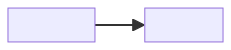
\includegraphics[keepaspectratio,alt={Start here, end here}]{example1.png}}
\caption{Start here, end here}
\end{figure}

Example generated with \emph{dia}:

\begin{verbatim}
<img src="./diag.png" alt="Disk feeding tape">
\end{verbatim}

\begin{figure}
\centering
\pandocbounded{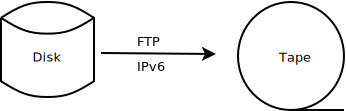
\includegraphics[keepaspectratio,alt={Disk feeding tape}]{diag.png}}
\caption{Disk feeding tape}
\end{figure}

Please add alternate text to help people with visual difficulties.

\emph{Note 4:} Direct use of \emph{mermaid} in markdown source is not
recommended, as it causes difficulty when generating a PDF version of
book6.

\emph{Note 5:} Earlier versions of this section recommended SVG format.
This has been removed since SVG causes difficulty when generating a PDF
version of book6.

Existing diagrams in JPG format can be inserted in the same way.

\subsubsection{\texorpdfstring{\hyperref[section-template]{Previous}
\hyperref[last-section]{Next}
\hyperref[chapter-template]{Top}}{Previous Next Top}}\label{previous-next-top-40}

\pagebreak

\subsection{Last Section}\label{last-section}

Section text goes here

\subsubsection{\texorpdfstring{\hyperref[markdown-usage]{Previous}
\hyperref[chapter-template]{Next}
\hyperref[chapter-template]{Top}}{Previous Next Top}}\label{previous-next-top-41}

\pagebreak

\section{book6 Main Index}\label{book6-main-index}

\begin{figure}
\centering
\pandocbounded{\includegraphics[keepaspectratio,alt={book6 logo}]{book6logo.png}}
\caption{book6 logo}
\end{figure}

Generated at 2026-02-12 16:00:42 UTC+1300

This index was created automatically, so it\textquotesingle s dumb. It
is not case-sensitive. It has links to each section that mentions each
keyword. If you think any keywords are missing, please raise an issue
(use link on GitHub toolbar).

\hyperref[dual-stack-scenarios]{464XLAT ¶}
\hyperref[translation-and-ipv4-as-a-service]{¶}
\hyperref[deployment-by-carriers]{¶}

\hyperref[tunnels]{6PE ¶}

\hyperref[obsolete-techniques]{6to4 ¶}

\hyperref[address-and-prefix-management]{address accountability ¶}

\hyperref[address-and-prefix-management]{address management ¶}

\hyperref[how-a-user-sees-ipv6]{address ¶}
\hyperref[how-an-application-programmer-sees-ipv6]{¶}
\hyperref[why-version-6]{¶} \hyperref[ipv6-basic-technology]{¶}
\hyperref[address-resolution]{¶} \hyperref[addresses]{¶}
\hyperref[auto-configuration]{¶} \hyperref[dns]{¶}
\hyperref[layer-2-functions]{¶} \hyperref[managed-configuration]{¶}
\hyperref[packet-format]{¶} \hyperref[routing]{¶}
\hyperref[source-and-destination-address-selection]{¶}
\hyperref[coexistence-with-legacy-ipv4]{¶}
\hyperref[dual-stack-scenarios]{¶}
\hyperref[ipv6-primary-differences-from-ipv4]{¶}
\hyperref[obsolete-techniques]{¶}
\hyperref[translation-and-ipv4-as-a-service]{¶} \hyperref[tunnels]{¶}
\hyperref[security]{¶} \hyperref[filtering]{¶}
\hyperref[layer-2-considerations]{¶} \hyperref[topology-obfuscation]{¶}
\hyperref[network-design]{¶} \hyperref[address-planning]{¶}
\hyperref[prefix-per-host]{¶}
\hyperref[address-and-prefix-management]{¶}
\hyperref[basic-windows-commands]{¶} \hyperref[energy-consumption]{¶}
\hyperref[multi-prefix-operation]{¶} \hyperref[multihoming]{¶}
\hyperref[routing-operation]{¶} \hyperref[security-operation]{¶}
\hyperref[cern-and-the-lhc]{¶} \hyperref[deployment-by-carriers]{¶}
\hyperref[deployment-in-the-enterprise]{¶}
\hyperref[deployment-in-the-home]{¶} \hyperref[troubleshooting]{¶}
\hyperref[advanced-troubleshooting]{¶} \hyperref[tools]{¶}
\hyperref[obsolete-features-in-ipv6]{¶} \hyperref[markdown-usage]{¶}

\hyperref[addresses]{anycast ¶}

\hyperref[address-resolution]{ARP ¶}
\hyperref[ipv6-primary-differences-from-ipv4]{¶}
\hyperref[layer-2-considerations]{¶} \hyperref[troubleshooting]{¶}

\hyperref[routing]{Babel ¶}

\hyperref[addresses]{BGP ¶} \hyperref[routing]{¶}
\hyperref[filtering]{¶} \hyperref[multi-prefix-operation]{¶}
\hyperref[multihoming]{¶} \hyperref[routing-operation]{¶}
\hyperref[tools]{¶} \hyperref[further-reading]{¶}

\hyperref[managed-configuration]{broadcast ¶}
\hyperref[ipv6-primary-differences-from-ipv4]{¶}

\hyperref[address-and-prefix-management]{BYOD ¶}

\hyperref[dual-stack-scenarios]{CGN ¶} \hyperref[obsolete-techniques]{¶}
\hyperref[tunnels]{¶}

\hyperref[coexistence-with-legacy-ipv4]{coexistence ¶}
\hyperref[dual-stack-scenarios]{¶} \hyperref[obsolete-techniques]{¶}
\hyperref[translation-and-ipv4-as-a-service]{¶} \hyperref[tunnels]{¶}
\hyperref[network-design]{¶} \hyperref[energy-consumption]{¶}
\hyperref[multihoming]{¶} \hyperref[security-operation]{¶}
\hyperref[obsolete-features-in-ipv6]{¶}

\hyperref[address-resolution]{DAD ¶} \hyperref[auto-configuration]{¶}
\hyperref[layer-2-considerations]{¶}
\hyperref[address-and-prefix-management]{¶}

\hyperref[auto-configuration]{DHCP ¶} \hyperref[dns]{¶}
\hyperref[managed-configuration]{¶} \hyperref[routing]{¶}
\hyperref[source-and-destination-address-selection]{¶}
\hyperref[dual-stack-scenarios]{¶}
\hyperref[ipv6-primary-differences-from-ipv4]{¶} \hyperref[filtering]{¶}
\hyperref[layer-2-considerations]{¶} \hyperref[address-planning]{¶}
\hyperref[prefix-per-host]{¶}
\hyperref[address-and-prefix-management]{¶}
\hyperref[multi-prefix-operation]{¶} \hyperref[cern-and-the-lhc]{¶}
\hyperref[troubleshooting]{¶} \hyperref[advanced-troubleshooting]{¶}

\hyperref[packet-format]{differentiated services ¶}
\hyperref[routing]{¶} \hyperref[traffic-class-and-flow-label]{¶}
\hyperref[transport-protocols]{¶}

\hyperref[dual-stack-scenarios]{DNS64 ¶}
\hyperref[translation-and-ipv4-as-a-service]{¶}
\hyperref[advanced-troubleshooting]{¶} \hyperref[tools]{¶}

\hyperref[how-an-application-programmer-sees-ipv6]{DNS ¶}
\hyperref[addresses]{¶} \hyperref[auto-configuration]{¶}
\hyperref[dns]{¶} \hyperref[managed-configuration]{¶}
\hyperref[dual-stack-scenarios]{¶}
\hyperref[translation-and-ipv4-as-a-service]{¶}
\hyperref[management-and-operations]{¶}
\hyperref[address-and-prefix-management]{¶}
\hyperref[benchmarking-and-monitoring]{¶}
\hyperref[multi-prefix-operation]{¶} \hyperref[multihoming]{¶}
\hyperref[deployment-in-the-enterprise]{¶}
\hyperref[deployment-in-the-home]{¶} \hyperref[status]{¶}
\hyperref[troubleshooting]{¶} \hyperref[advanced-troubleshooting]{¶}
\hyperref[tools]{¶}

\hyperref[dual-stack-scenarios]{DS-Lite ¶}
\hyperref[translation-and-ipv4-as-a-service]{¶} \hyperref[tunnels]{¶}

\hyperref[how-an-application-programmer-sees-ipv6]{dual stack ¶}
\hyperref[routing]{¶} \hyperref[transport-protocols]{¶}
\hyperref[coexistence-with-legacy-ipv4]{¶}
\hyperref[dual-stack-scenarios]{¶}
\hyperref[translation-and-ipv4-as-a-service]{¶} \hyperref[tunnels]{¶}
\hyperref[network-design]{¶} \hyperref[address-and-prefix-management]{¶}
\hyperref[energy-consumption]{¶} \hyperref[cern-and-the-lhc]{¶}
\hyperref[deployment-in-the-home]{¶} \hyperref[troubleshooting]{¶}
\hyperref[advanced-troubleshooting]{¶}

\hyperref[packet-format]{ECN ¶}
\hyperref[traffic-class-and-flow-label]{¶}
\hyperref[transport-protocols]{¶}

\hyperref[layer-2-functions]{encapsulation ¶}
\hyperref[dual-stack-scenarios]{¶}
\hyperref[translation-and-ipv4-as-a-service]{¶} \hyperref[tunnels]{¶}

\hyperref[layer-2-functions]{Ethertype ¶}

\hyperref[extension-headers-and-options]{firewall ¶}
\hyperref[dual-stack-scenarios]{¶} \hyperref[security]{¶}
\hyperref[topology-obfuscation]{¶} \hyperref[network-design]{¶}
\hyperref[address-and-prefix-management]{¶}
\hyperref[benchmarking-and-monitoring]{¶} \hyperref[multihoming]{¶}
\hyperref[advanced-troubleshooting]{¶}

\hyperref[packet-format]{flow label ¶} \hyperref[routing]{¶}
\hyperref[traffic-class-and-flow-label]{¶} \hyperref[markdown-usage]{¶}

\hyperref[how-an-application-programmer-sees-ipv6]{getaddrinfo ¶}
\hyperref[dns]{¶} \hyperref[dual-stack-scenarios]{¶}

\hyperref[layer-2-functions]{GRE ¶} \hyperref[tunnels]{¶}

\hyperref[addresses]{GUA ¶} \hyperref[auto-configuration]{¶}
\hyperref[source-and-destination-address-selection]{¶}
\hyperref[ipv6-primary-differences-from-ipv4]{¶}
\hyperref[translation-and-ipv4-as-a-service]{¶}
\hyperref[topology-obfuscation]{¶} \hyperref[address-planning]{¶}
\hyperref[multi-prefix-operation]{¶}

\hyperref[how-an-application-programmer-sees-ipv6]{happy eyeballs ¶}
\hyperref[multihoming]{¶} \hyperref[deployment-in-the-home]{¶}
\hyperref[troubleshooting]{¶} \hyperref[advanced-troubleshooting]{¶}

\hyperref[why-version-6]{IANA ¶} \hyperref[addresses]{¶}
\hyperref[auto-configuration]{¶}
\hyperref[extension-headers-and-options]{¶}
\hyperref[managed-configuration]{¶} \hyperref[packet-format]{¶}
\hyperref[filtering]{¶} \hyperref[obsolete-features-in-ipv6]{¶}

\hyperref[address-resolution]{ICMPv6 ¶} \hyperref[auto-configuration]{¶}
\hyperref[extension-headers-and-options]{¶}
\hyperref[dual-stack-scenarios]{¶}
\hyperref[translation-and-ipv4-as-a-service]{¶} \hyperref[security]{¶}
\hyperref[filtering]{¶} \hyperref[troubleshooting]{¶}
\hyperref[advanced-troubleshooting]{¶}

\hyperref[addresses]{IID ¶}
\hyperref[ipv6-primary-differences-from-ipv4]{¶}
\hyperref[translation-and-ipv4-as-a-service]{¶}
\hyperref[layer-2-considerations]{¶}
\hyperref[multi-prefix-operation]{¶} \hyperref[multihoming]{¶}

\hyperref[address-and-prefix-management]{IPAM ¶}

\hyperref[extension-headers-and-options]{IPsec ¶}
\hyperref[packet-format]{¶} \hyperref[security]{¶}

\hyperref[coexistence-with-legacy-ipv4]{IPv4 as a Service ¶}
\hyperref[dual-stack-scenarios]{¶}
\hyperref[translation-and-ipv4-as-a-service]{¶}
\hyperref[network-design]{¶} \hyperref[multihoming]{¶}
\hyperref[deployment-in-the-home]{¶}

\hyperref[how-a-network-operations-center-sees-ipv6]{IPv4 ¶}
\hyperref[how-an-application-programmer-sees-ipv6]{¶}
\hyperref[why-version-6]{¶} \hyperref[address-resolution]{¶}
\hyperref[addresses]{¶} \hyperref[dns]{¶}
\hyperref[extension-headers-and-options]{¶}
\hyperref[layer-2-functions]{¶} \hyperref[managed-configuration]{¶}
\hyperref[routing]{¶}
\hyperref[source-and-destination-address-selection]{¶}
\hyperref[traffic-class-and-flow-label]{¶}
\hyperref[transport-protocols]{¶}
\hyperref[coexistence-with-legacy-ipv4]{¶}
\hyperref[dual-stack-scenarios]{¶}
\hyperref[ipv6-primary-differences-from-ipv4]{¶}
\hyperref[obsolete-techniques]{¶}
\hyperref[translation-and-ipv4-as-a-service]{¶} \hyperref[tunnels]{¶}
\hyperref[security]{¶} \hyperref[filtering]{¶}
\hyperref[layer-2-considerations]{¶} \hyperref[topology-obfuscation]{¶}
\hyperref[network-design]{¶} \hyperref[address-planning]{¶}
\hyperref[address-and-prefix-management]{¶}
\hyperref[benchmarking-and-monitoring]{¶}
\hyperref[energy-consumption]{¶} \hyperref[multi-prefix-operation]{¶}
\hyperref[multihoming]{¶} \hyperref[packet-size-and-jumbo-frames]{¶}
\hyperref[routing-operation]{¶} \hyperref[cern-and-the-lhc]{¶}
\hyperref[deployment-by-carriers]{¶}
\hyperref[deployment-in-the-home]{¶} \hyperref[status]{¶}
\hyperref[troubleshooting]{¶} \hyperref[advanced-troubleshooting]{¶}
\hyperref[tools]{¶} \hyperref[obsolete-features-in-ipv6]{¶}
\hyperref[further-reading]{¶}

\hyperref[dual-stack-scenarios]{IPv6-mostly ¶}

\hyperref[routing]{IPv6-only ¶}
\hyperref[source-and-destination-address-selection]{¶}
\hyperref[coexistence-with-legacy-ipv4]{¶}
\hyperref[dual-stack-scenarios]{¶}
\hyperref[translation-and-ipv4-as-a-service]{¶} \hyperref[tunnels]{¶}
\hyperref[security]{¶} \hyperref[cern-and-the-lhc]{¶}
\hyperref[deployment-by-carriers]{¶}
\hyperref[advanced-troubleshooting]{¶}

\hyperref[routing]{IS-IS ¶} \hyperref[routing-operation]{¶}

\hyperref[addresses]{ISP ¶} \hyperref[routing]{¶}
\hyperref[dual-stack-scenarios]{¶}
\hyperref[translation-and-ipv4-as-a-service]{¶} \hyperref[tunnels]{¶}
\hyperref[address-planning]{¶}
\hyperref[address-and-prefix-management]{¶}
\hyperref[multi-prefix-operation]{¶} \hyperref[multihoming]{¶}
\hyperref[deployment-in-the-enterprise]{¶}
\hyperref[deployment-in-the-home]{¶}

\hyperref[packet-size-and-jumbo-frames]{Jumbo frames ¶}

\hyperref[address-resolution]{link-local ¶} \hyperref[addresses]{¶}
\hyperref[auto-configuration]{¶} \hyperref[dns]{¶}
\hyperref[source-and-destination-address-selection]{¶}
\hyperref[filtering]{¶} \hyperref[network-design]{¶}
\hyperref[basic-windows-commands]{¶} \hyperref[energy-consumption]{¶}
\hyperref[multi-prefix-operation]{¶}
\hyperref[deployment-in-the-home]{¶} \hyperref[troubleshooting]{¶}
\hyperref[tools]{¶}

\hyperref[addresses]{loopback ¶}

\hyperref[translation-and-ipv4-as-a-service]{Lw6o4 ¶}

\hyperref[address-resolution]{MAC address ¶} \hyperref[addresses]{¶}
\hyperref[address-and-prefix-management]{¶}

\hyperref[translation-and-ipv4-as-a-service]{MAP ¶}

\hyperref[address-resolution]{MLD ¶}
\hyperref[layer-2-considerations]{¶} \hyperref[troubleshooting]{¶}
\hyperref[advanced-troubleshooting]{¶}

\hyperref[layer-2-functions]{MPLS ¶} \hyperref[tunnels]{¶}

\hyperref[transport-protocols]{MPTCP ¶} \hyperref[multihoming]{¶}

\hyperref[extension-headers-and-options]{MTU ¶}
\hyperref[layer-2-functions]{¶} \hyperref[packet-format]{¶}
\hyperref[packet-size-and-jumbo-frames]{¶}
\hyperref[advanced-troubleshooting]{¶}

\hyperref[address-resolution]{multicast ¶} \hyperref[addresses]{¶}
\hyperref[auto-configuration]{¶} \hyperref[layer-2-functions]{¶}
\hyperref[ipv6-primary-differences-from-ipv4]{¶} \hyperref[filtering]{¶}
\hyperref[layer-2-considerations]{¶} \hyperref[energy-consumption]{¶}
\hyperref[troubleshooting]{¶} \hyperref[advanced-troubleshooting]{¶}

\hyperref[multi-prefix-operation]{multihoming ¶}
\hyperref[multihoming]{¶} \hyperref[deployment-in-the-enterprise]{¶}

\hyperref[translation-and-ipv4-as-a-service]{NAT464 ¶}

\hyperref[dual-stack-scenarios]{NAT64 ¶}
\hyperref[obsolete-techniques]{¶}
\hyperref[translation-and-ipv4-as-a-service]{¶}
\hyperref[advanced-troubleshooting]{¶} \hyperref[tools]{¶}

\hyperref[ipv6-primary-differences-from-ipv4]{NAT66 ¶}
\hyperref[translation-and-ipv4-as-a-service]{¶} \hyperref[security]{¶}

\hyperref[transport-protocols]{NAT ¶} \hyperref[dual-stack-scenarios]{¶}
\hyperref[obsolete-techniques]{¶}
\hyperref[translation-and-ipv4-as-a-service]{¶} \hyperref[tunnels]{¶}
\hyperref[security]{¶} \hyperref[topology-obfuscation]{¶}
\hyperref[address-planning]{¶} \hyperref[multihoming]{¶}
\hyperref[deployment-in-the-enterprise]{¶}

\hyperref[address-resolution]{neighbor discovery ¶}
\hyperref[auto-configuration]{¶} \hyperref[managed-configuration]{¶}
\hyperref[layer-2-considerations]{¶}
\hyperref[address-and-prefix-management]{¶}
\hyperref[troubleshooting]{¶} \hyperref[advanced-troubleshooting]{¶}
\hyperref[tools]{¶} \hyperref[obsolete-features-in-ipv6]{¶}

\hyperref[translation-and-ipv4-as-a-service]{NPTv6 ¶}
\hyperref[security]{¶} \hyperref[multihoming]{¶}

\hyperref[how-to-keep-up-to-date]{obsolete ¶} \hyperref[addresses]{¶}
\hyperref[dns]{¶} \hyperref[obsolete-techniques]{¶}
\hyperref[tunnels]{¶} \hyperref[obsolete-features-in-ipv6]{¶}
\hyperref[further-reading]{¶}

\hyperref[routing]{OSPF ¶} \hyperref[routing-operation]{¶}

\hyperref[dual-stack-scenarios]{performance ¶}
\hyperref[ipv6-primary-differences-from-ipv4]{¶} \hyperref[filtering]{¶}
\hyperref[network-design]{¶} \hyperref[management-and-operations]{¶}
\hyperref[multihoming]{¶} \hyperref[packet-size-and-jumbo-frames]{¶}
\hyperref[troubleshooting]{¶} \hyperref[advanced-troubleshooting]{¶}
\hyperref[tools]{¶}

\hyperref[auto-configuration]{PIO ¶}

\hyperref[extension-headers-and-options]{PMTUD ¶}
\hyperref[filtering]{¶} \hyperref[packet-size-and-jumbo-frames]{¶}

\hyperref[layer-2-functions]{PPP ¶}

\hyperref[managed-configuration]{prefix delegation ¶}
\hyperref[prefix-per-host]{¶}
\hyperref[address-and-prefix-management]{¶}

\hyperref[addresses]{prefix ¶} \hyperref[auto-configuration]{¶}
\hyperref[managed-configuration]{¶} \hyperref[routing]{¶}
\hyperref[source-and-destination-address-selection]{¶}
\hyperref[dual-stack-scenarios]{¶}
\hyperref[ipv6-primary-differences-from-ipv4]{¶}
\hyperref[translation-and-ipv4-as-a-service]{¶} \hyperref[tunnels]{¶}
\hyperref[security]{¶} \hyperref[filtering]{¶}
\hyperref[layer-2-considerations]{¶} \hyperref[topology-obfuscation]{¶}
\hyperref[network-design]{¶} \hyperref[address-planning]{¶}
\hyperref[prefix-per-host]{¶}
\hyperref[address-and-prefix-management]{¶}
\hyperref[multi-prefix-operation]{¶} \hyperref[multihoming]{¶}
\hyperref[advanced-troubleshooting]{¶}
\hyperref[obsolete-features-in-ipv6]{¶}

\hyperref[addresses]{privacy ¶} \hyperref[auto-configuration]{¶}
\hyperref[source-and-destination-address-selection]{¶}
\hyperref[ipv6-primary-differences-from-ipv4]{¶} \hyperref[security]{¶}
\hyperref[layer-2-considerations]{¶}
\hyperref[basic-windows-commands]{¶}
\hyperref[multi-prefix-operation]{¶} \hyperref[security-operation]{¶}

\hyperref[transport-protocols]{QUIC ¶} \hyperref[multihoming]{¶}

\hyperref[address-resolution]{RA messages ¶}
\hyperref[auto-configuration]{¶} \hyperref[managed-configuration]{¶}
\hyperref[routing]{¶} \hyperref[prefix-per-host]{¶}
\hyperref[multi-prefix-operation]{¶}
\hyperref[advanced-troubleshooting]{¶} \hyperref[tools]{¶}
\hyperref[obsolete-features-in-ipv6]{¶}

\hyperref[addresses]{registry ¶} \hyperref[auto-configuration]{¶}
\hyperref[extension-headers-and-options]{¶} \hyperref[filtering]{¶}
\hyperref[address-planning]{¶} \hyperref[multi-prefix-operation]{¶}
\hyperref[multihoming]{¶} \hyperref[deployment-in-the-enterprise]{¶}
\hyperref[status]{¶}

\hyperref[dns]{reverse DNS ¶}

\hyperref[routing]{RIPng ¶}

\hyperref[why-version-6]{route ¶} \hyperref[ipv6-basic-technology]{¶}
\hyperref[address-resolution]{¶} \hyperref[addresses]{¶}
\hyperref[auto-configuration]{¶} \hyperref[dns]{¶}
\hyperref[extension-headers-and-options]{¶}
\hyperref[layer-2-functions]{¶} \hyperref[managed-configuration]{¶}
\hyperref[packet-format]{¶} \hyperref[routing]{¶}
\hyperref[traffic-class-and-flow-label]{¶}
\hyperref[coexistence-with-legacy-ipv4]{¶}
\hyperref[dual-stack-scenarios]{¶}
\hyperref[ipv6-primary-differences-from-ipv4]{¶}
\hyperref[translation-and-ipv4-as-a-service]{¶} \hyperref[tunnels]{¶}
\hyperref[filtering]{¶} \hyperref[layer-2-considerations]{¶}
\hyperref[topology-obfuscation]{¶} \hyperref[network-design]{¶}
\hyperref[address-planning]{¶} \hyperref[management-and-operations]{¶}
\hyperref[address-and-prefix-management]{¶}
\hyperref[energy-consumption]{¶} \hyperref[multi-prefix-operation]{¶}
\hyperref[multihoming]{¶} \hyperref[packet-size-and-jumbo-frames]{¶}
\hyperref[routing-operation]{¶} \hyperref[security-operation]{¶}
\hyperref[deployment-by-carriers]{¶}
\hyperref[deployment-in-the-enterprise]{¶}
\hyperref[deployment-in-the-home]{¶} \hyperref[troubleshooting]{¶}
\hyperref[advanced-troubleshooting]{¶} \hyperref[tools]{¶}
\hyperref[obsolete-features-in-ipv6]{¶} \hyperref[further-reading]{¶}

\hyperref[routing]{RPL ¶}

\hyperref[transport-protocols]{RTP ¶}

\hyperref[transport-protocols]{SCTP ¶}

\hyperref[dns]{security ¶} \hyperref[extension-headers-and-options]{¶}
\hyperref[managed-configuration]{¶} \hyperref[packet-format]{¶}
\hyperref[source-and-destination-address-selection]{¶}
\hyperref[dual-stack-scenarios]{¶}
\hyperref[ipv6-primary-differences-from-ipv4]{¶}
\hyperref[obsolete-techniques]{¶}
\hyperref[translation-and-ipv4-as-a-service]{¶} \hyperref[security]{¶}
\hyperref[filtering]{¶} \hyperref[layer-2-considerations]{¶}
\hyperref[topology-obfuscation]{¶}
\hyperref[address-and-prefix-management]{¶}
\hyperref[multi-prefix-operation]{¶} \hyperref[security-operation]{¶}
\hyperref[deployment-in-the-enterprise]{¶}
\hyperref[obsolete-features-in-ipv6]{¶} \hyperref[further-reading]{¶}

\hyperref[why-version-6]{SIP ¶} \hyperref[transport-protocols]{¶}
\hyperref[dual-stack-scenarios]{¶}
\hyperref[translation-and-ipv4-as-a-service]{¶}
\hyperref[multihoming]{¶}

\hyperref[auto-configuration]{SLAAC ¶}
\hyperref[managed-configuration]{¶} \hyperref[routing]{¶}
\hyperref[ipv6-primary-differences-from-ipv4]{¶} \hyperref[security]{¶}
\hyperref[filtering]{¶} \hyperref[layer-2-considerations]{¶}
\hyperref[address-and-prefix-management]{¶}
\hyperref[multi-prefix-operation]{¶}

\hyperref[transport-protocols]{STUN ¶}

\hyperref[why-version-6]{TCP ¶} \hyperref[addresses]{¶}
\hyperref[extension-headers-and-options]{¶} \hyperref[packet-format]{¶}
\hyperref[traffic-class-and-flow-label]{¶}
\hyperref[transport-protocols]{¶} \hyperref[multihoming]{¶}

\hyperref[obsolete-techniques]{Teredo ¶}

\hyperref[layer-2-functions]{tunnel ¶}
\hyperref[traffic-class-and-flow-label]{¶}
\hyperref[coexistence-with-legacy-ipv4]{¶}
\hyperref[dual-stack-scenarios]{¶} \hyperref[obsolete-techniques]{¶}
\hyperref[tunnels]{¶} \hyperref[layer-2-considerations]{¶}

\hyperref[extension-headers-and-options]{UDP ¶}
\hyperref[managed-configuration]{¶} \hyperref[packet-format]{¶}
\hyperref[transport-protocols]{¶} \hyperref[obsolete-techniques]{¶}

\hyperref[addresses]{ULA ¶} \hyperref[auto-configuration]{¶}
\hyperref[dns]{¶} \hyperref[source-and-destination-address-selection]{¶}
\hyperref[ipv6-primary-differences-from-ipv4]{¶}
\hyperref[translation-and-ipv4-as-a-service]{¶} \hyperref[filtering]{¶}
\hyperref[topology-obfuscation]{¶} \hyperref[multi-prefix-operation]{¶}
\hyperref[multihoming]{¶}

\hyperref[address-resolution]{wireless ¶}
\hyperref[auto-configuration]{¶} \hyperref[layer-2-functions]{¶}
\hyperref[managed-configuration]{¶} \hyperref[routing]{¶}
\hyperref[ipv6-primary-differences-from-ipv4]{¶}
\hyperref[layer-2-considerations]{¶} \hyperref[network-design]{¶}
\hyperref[address-planning]{¶} \hyperref[prefix-per-host]{¶}
\hyperref[address-and-prefix-management]{¶}
\hyperref[multi-prefix-operation]{¶} \hyperref[multihoming]{¶}
\hyperref[deployment-by-carriers]{¶}
\hyperref[deployment-in-the-home]{¶}
\hyperref[advanced-troubleshooting]{¶}

\subsubsection{\texorpdfstring{\hyperref[list-of-contents]{Back to main
Contents}}{Back to main Contents}}\label{back-to-main-contents-12}

\pagebreak

\section{book6 Citation Index}\label{book6-citation-index}

\begin{figure}
\centering
\pandocbounded{\includegraphics[keepaspectratio,alt={book6 logo}]{book6logo.png}}
\caption{book6 logo}
\end{figure}

Generated at 2026-02-12 16:00:42 UTC+1300

This index was created automatically, so it\textquotesingle s dumb. It
has links to each section that mentions each citation.

\hyperref[addresses]{BCP157 ¶}

\hyperref[coexistence-with-legacy-ipv4]{BCP177 ¶}

\hyperref[addresses]{BCP198 ¶} \hyperref[routing]{¶}
\hyperref[markdown-usage]{¶}

\hyperref[energy-consumption]{BCP202 ¶}

\hyperref[ipv6-basic-technology]{BCP220 ¶} \hyperref[further-reading]{¶}

\hyperref[extension-headers-and-options]{BCP230 ¶}

\hyperref[filtering]{BCP38 ¶}

\hyperref[multi-prefix-operation]{BCP84 ¶}

\hyperref[dns]{BCP91 ¶}

\hyperref[why-version-6]{RFC1190 ¶}

\hyperref[why-version-6]{RFC1475 ¶}

\hyperref[why-version-6]{RFC1606 ¶}

\hyperref[why-version-6]{RFC1700 ¶}

\hyperref[why-version-6]{RFC1819 ¶}

\hyperref[why-version-6]{RFC1883 ¶}

\hyperref[dual-stack-scenarios]{RFC1918 ¶} \hyperref[tunnels]{¶}
\hyperref[obsolete-features-in-ipv6]{¶}

\hyperref[routing]{RFC2080 ¶}

\hyperref[routing]{RFC2081 ¶}

\hyperref[layer-2-functions]{RFC2464 ¶}

\hyperref[packet-format]{RFC2474 ¶}
\hyperref[traffic-class-and-flow-label]{¶}
\hyperref[transport-protocols]{¶}

\hyperref[obsolete-techniques]{RFC2529 ¶}

\hyperref[routing]{RFC2545 ¶} \hyperref[routing-operation]{¶}

\hyperref[packet-size-and-jumbo-frames]{RFC2675 ¶}

\hyperref[obsolete-techniques]{RFC3053 ¶}

\hyperref[obsolete-techniques]{RFC3056 ¶}

\hyperref[obsolete-techniques]{RFC3068 ¶}

\hyperref[obsolete-techniques]{RFC3089 ¶}

\hyperref[packet-format]{RFC3168 ¶}
\hyperref[traffic-class-and-flow-label]{¶}
\hyperref[transport-protocols]{¶}

\hyperref[transport-protocols]{RFC3261 ¶}

\hyperref[source-and-destination-address-selection]{RFC3484 ¶}

\hyperref[obsolete-features-in-ipv6]{RFC3513 ¶}
\hyperref[markdown-usage]{¶}

\hyperref[dual-stack-scenarios]{RFC3542 ¶}

\hyperref[transport-protocols]{RFC3550 ¶}

\hyperref[multihoming]{RFC3582 ¶}

\hyperref[addresses]{RFC3587 ¶}

\hyperref[dns]{RFC3596 ¶}

\hyperref[managed-configuration]{RFC3633 ¶}

\hyperref[layer-2-considerations]{RFC3756 ¶}

\hyperref[address-resolution]{RFC3810 ¶}

\hyperref[transport-protocols]{RFC3828 ¶}

\hyperref[addresses]{RFC3849 ¶}

\hyperref[addresses]{RFC3879 ¶} \hyperref[obsolete-features-in-ipv6]{¶}

\hyperref[security]{RFC3971 ¶} \hyperref[layer-2-considerations]{¶}
\hyperref[obsolete-features-in-ipv6]{¶}

\hyperref[addresses]{RFC4007 ¶}

\hyperref[layer-2-functions]{RFC4029 ¶} \hyperref[tunnels]{¶}

\hyperref[addresses]{RFC4038 ¶}

\hyperref[addresses]{RFC4048 ¶}

\hyperref[filtering]{RFC4193 ¶} \hyperref[multihoming]{¶}

\hyperref[dual-stack-scenarios]{RFC4213 ¶} \hyperref[tunnels]{¶}

\hyperref[routing]{RFC4271 ¶} \hyperref[routing-operation]{¶}

\hyperref[obsolete-features-in-ipv6]{RFC4283 ¶}

\hyperref[obsolete-features-in-ipv6]{RFC4285 ¶}

\hyperref[address-resolution]{RFC4291 ¶} \hyperref[addresses]{¶}
\hyperref[filtering]{¶} \hyperref[obsolete-features-in-ipv6]{¶}
\hyperref[markdown-usage]{¶}

\hyperref[security]{RFC4301 ¶}

\hyperref[extension-headers-and-options]{RFC4303 ¶}
\hyperref[packet-format]{¶}

\hyperref[obsolete-techniques]{RFC4380 ¶}

\hyperref[routing]{RFC4456 ¶} \hyperref[routing-operation]{¶}

\hyperref[address-resolution]{RFC4541 ¶}
\hyperref[layer-2-considerations]{¶}

\hyperref[traffic-class-and-flow-label]{RFC4594 ¶}

\hyperref[filtering]{RFC4641 ¶}

\hyperref[routing]{RFC4760 ¶} \hyperref[routing-operation]{¶}

\hyperref[tunnels]{RFC4798 ¶}

\hyperref[address-resolution]{RFC4861 ¶}
\hyperref[auto-configuration]{¶}

\hyperref[auto-configuration]{RFC4862 ¶}
\hyperref[address-and-prefix-management]{¶}

\hyperref[topology-obfuscation]{RFC4864 ¶}

\hyperref[filtering]{RFC4890 ¶}

\hyperref[transport-protocols]{RFC4960 ¶}

\hyperref[layer-2-functions]{RFC5072 ¶}

\hyperref[filtering]{RFC5082 ¶}

\hyperref[traffic-class-and-flow-label]{RFC5127 ¶}

\hyperref[layer-2-functions]{RFC5172 ¶}

\hyperref[obsolete-techniques]{RFC5214 ¶}

\hyperref[routing]{RFC5308 ¶} \hyperref[routing-operation]{¶}

\hyperref[routing]{RFC5340 ¶} \hyperref[routing-operation]{¶}

\hyperref[multihoming]{RFC5533 ¶}

\hyperref[obsolete-techniques]{RFC5569 ¶}

\hyperref[filtering]{RFC5635 ¶}

\hyperref[address-resolution]{RFC5757 ¶}

\hyperref[traffic-class-and-flow-label]{RFC5865 ¶}

\hyperref[translation-and-ipv4-as-a-service]{RFC5902 ¶}

\hyperref[auto-configuration]{RFC5942 ¶}

\hyperref[addresses]{RFC5952 ¶}

\hyperref[tunnels]{RFC5969 ¶}

\hyperref[layer-2-functions]{RFC6085 ¶}

\hyperref[layer-2-considerations]{RFC6105 ¶}
\hyperref[obsolete-features-in-ipv6]{¶}

\hyperref[translation-and-ipv4-as-a-service]{RFC6144 ¶}

\hyperref[translation-and-ipv4-as-a-service]{RFC6146 ¶}

\hyperref[translation-and-ipv4-as-a-service]{RFC6147 ¶}

\hyperref[dual-stack-scenarios]{RFC6157 ¶} \hyperref[multihoming]{¶}

\hyperref[address-planning]{RFC6177 ¶}

\hyperref[coexistence-with-legacy-ipv4]{RFC6180 ¶}

\hyperref[filtering]{RFC6192 ¶}

\hyperref[obsolete-techniques]{RFC6264 ¶} \hyperref[tunnels]{¶}

\hyperref[obsolete-features-in-ipv6]{RFC6275 ¶}

\hyperref[translation-and-ipv4-as-a-service]{RFC6296 ¶}
\hyperref[security]{¶} \hyperref[multihoming]{¶}

\hyperref[translation-and-ipv4-as-a-service]{RFC6314 ¶}
\hyperref[multihoming]{¶}

\hyperref[dual-stack-scenarios]{RFC6333 ¶}
\hyperref[translation-and-ipv4-as-a-service]{¶} \hyperref[tunnels]{¶}

\hyperref[obsolete-techniques]{RFC6343 ¶}

\hyperref[traffic-class-and-flow-label]{RFC6437 ¶}

\hyperref[traffic-class-and-flow-label]{RFC6438 ¶}

\hyperref[obsolete-features-in-ipv6]{RFC6494 ¶}

\hyperref[obsolete-features-in-ipv6]{RFC6495 ¶}

\hyperref[routing]{RFC6550 ¶}

\hyperref[address-resolution]{RFC6583 ¶}
\hyperref[layer-2-considerations]{¶}

\hyperref[address-planning]{RFC6598 ¶}

\hyperref[layer-2-considerations]{RFC6620 ¶}

\hyperref[address-resolution]{RFC6636 ¶}

\hyperref[addresses]{RFC6666 ¶} \hyperref[filtering]{¶}

\hyperref[how-an-application-programmer-sees-ipv6]{RFC6724 ¶}
\hyperref[dns]{¶} \hyperref[source-and-destination-address-selection]{¶}
\hyperref[multi-prefix-operation]{¶}
\hyperref[obsolete-features-in-ipv6]{¶}

\hyperref[obsolete-techniques]{RFC6751 ¶}

\hyperref[address-resolution]{RFC6775 ¶}

\hyperref[dual-stack-scenarios]{RFC6877 ¶}
\hyperref[translation-and-ipv4-as-a-service]{¶}

\hyperref[dual-stack-scenarios]{RFC6888 ¶}

\hyperref[addresses]{RFC6890 ¶} \hyperref[filtering]{¶}

\hyperref[transport-protocols]{RFC6936 ¶}

\hyperref[multi-prefix-operation]{RFC6950 ¶}

\hyperref[obsolete-features-in-ipv6]{RFC6980 ¶}

\hyperref[filtering]{RFC7045 ¶}

\hyperref[obsolete-techniques]{RFC7050 ¶}

\hyperref[managed-configuration]{RFC7066 ¶}

\hyperref[dns]{RFC7078 ¶}
\hyperref[source-and-destination-address-selection]{¶}
\hyperref[multi-prefix-operation]{¶}

\hyperref[routing]{RFC7084 ¶}

\hyperref[traffic-class-and-flow-label]{RFC7098 ¶}
\hyperref[topology-obfuscation]{¶}

\hyperref[layer-2-considerations]{RFC7112 ¶}

\hyperref[layer-2-considerations]{RFC7113 ¶}
\hyperref[obsolete-features-in-ipv6]{¶}

\hyperref[filtering]{RFC7123 ¶}

\hyperref[multihoming]{RFC7157 ¶}

\hyperref[security-operation]{RFC7217 ¶}

\hyperref[tunnels]{RFC7439 ¶}

\hyperref[filtering]{RFC7454 ¶}

\hyperref[obsolete-techniques]{RFC7526 ¶}

\hyperref[auto-configuration]{RFC7527 ¶}

\hyperref[tunnels]{RFC7552 ¶}

\hyperref[multihoming]{RFC7556 ¶}

\hyperref[dual-stack-scenarios]{RFC7596 ¶}
\hyperref[translation-and-ipv4-as-a-service]{¶}

\hyperref[dual-stack-scenarios]{RFC7597 ¶}
\hyperref[translation-and-ipv4-as-a-service]{¶}

\hyperref[dual-stack-scenarios]{RFC7599 ¶}
\hyperref[translation-and-ipv4-as-a-service]{¶}

\hyperref[layer-2-considerations]{RFC7610 ¶}

\hyperref[why-version-6]{RFC762 ¶}

\hyperref[layer-2-functions]{RFC7676 ¶} \hyperref[tunnels]{¶}

\hyperref[transport-protocols]{RFC768 ¶}

\hyperref[extension-headers-and-options]{RFC7690 ¶}
\hyperref[packet-size-and-jumbo-frames]{¶}

\hyperref[security-operation]{RFC7721 ¶}

\hyperref[routing]{RFC7775 ¶} \hyperref[routing-operation]{¶}

\hyperref[layer-2-considerations]{RFC7849 ¶}

\hyperref[extension-headers-and-options]{RFC7872 ¶}

\hyperref[translation-and-ipv4-as-a-service]{RFC7915 ¶}

\hyperref[why-version-6]{RFC791 ¶}
\hyperref[traffic-class-and-flow-label]{¶}

\hyperref[security-operation]{RFC7943 ¶}

\hyperref[auto-configuration]{RFC8028 ¶}
\hyperref[multi-prefix-operation]{¶}

\hyperref[addresses]{RFC8064 ¶} \hyperref[auto-configuration]{¶}
\hyperref[layer-2-functions]{¶}

\hyperref[traffic-class-and-flow-label]{RFC8100 ¶}

\hyperref[auto-configuration]{RFC8106 ¶}

\hyperref[how-to-keep-up-to-date]{RFC8200 ¶}
\hyperref[ipv6-basic-technology]{¶} \hyperref[address-resolution]{¶}
\hyperref[extension-headers-and-options]{¶} \hyperref[packet-format]{¶}
\hyperref[filtering]{¶} \hyperref[further-reading]{¶}
\hyperref[markdown-usage]{¶}

\hyperref[packet-size-and-jumbo-frames]{RFC8201 ¶}

\hyperref[filtering]{RFC8210 ¶}

\hyperref[prefix-per-host]{RFC8273 ¶}

\hyperref[transport-protocols]{RFC8304 ¶}

\hyperref[how-an-application-programmer-sees-ipv6]{RFC8305 ¶}
\hyperref[dual-stack-scenarios]{¶} \hyperref[multihoming]{¶}
\hyperref[deployment-in-the-home]{¶}

\hyperref[layer-2-functions]{RFC8376 ¶} \hyperref[energy-consumption]{¶}

\hyperref[managed-configuration]{RFC8415 ¶}
\hyperref[address-planning]{¶} \hyperref[prefix-per-host]{¶}

\hyperref[multi-prefix-operation]{RFC8475 ¶}

\hyperref[dns]{RFC8501 ¶}

\hyperref[address-resolution]{RFC8505 ¶}

\hyperref[routing]{RFC8585 ¶} \hyperref[dual-stack-scenarios]{¶}

\hyperref[traffic-class-and-flow-label]{RFC8622 ¶}

\hyperref[multi-prefix-operation]{RFC8678 ¶}

\hyperref[translation-and-ipv4-as-a-service]{RFC8683 ¶}

\hyperref[transport-protocols]{RFC8684 ¶} \hyperref[multihoming]{¶}

\hyperref[energy-consumption]{RFC8724 ¶}

\hyperref[extension-headers-and-options]{RFC8754 ¶}

\hyperref[translation-and-ipv4-as-a-service]{RFC8781 ¶}

\hyperref[traffic-class-and-flow-label]{RFC8837 ¶}

\hyperref[translation-and-ipv4-as-a-service]{RFC8880 ¶}

\hyperref[extension-headers-and-options]{RFC8899 ¶}

\hyperref[dual-stack-scenarios]{RFC8925 ¶}

\hyperref[address-resolution]{RFC8928 ¶}

\hyperref[address-resolution]{RFC8929 ¶}

\hyperref[routing]{RFC8950 ¶}

\hyperref[routing]{RFC8966 ¶}

\hyperref[addresses]{RFC8981 ¶} \hyperref[auto-configuration]{¶}
\hyperref[layer-2-considerations]{¶} \hyperref[topology-obfuscation]{¶}
\hyperref[prefix-per-host]{¶}
\hyperref[address-and-prefix-management]{¶}
\hyperref[multi-prefix-operation]{¶} \hyperref[security-operation]{¶}

\hyperref[transport-protocols]{RFC9000 ¶}

\hyperref[routing]{RFC9008 ¶}

\hyperref[routing]{RFC9010 ¶}

\hyperref[routing]{RFC9096 ¶}

\hyperref[extension-headers-and-options]{RFC9098 ¶}

\hyperref[security]{RFC9099 ¶}
\hyperref[address-and-prefix-management]{¶}
\hyperref[security-operation]{¶}

\hyperref[address-resolution]{RFC9119 ¶} \hyperref[layer-2-functions]{¶}

\hyperref[address-resolution]{RFC9131 ¶}

\hyperref[extension-headers-and-options]{RFC9288 ¶}
\hyperref[filtering]{¶} \hyperref[security-operation]{¶}

\hyperref[coexistence-with-legacy-ipv4]{RFC9313 ¶}
\hyperref[dual-stack-scenarios]{¶}
\hyperref[translation-and-ipv4-as-a-service]{¶}

\hyperref[dual-stack-scenarios]{RFC9386 ¶}
\hyperref[deployment-by-carriers]{¶}
\hyperref[deployment-in-the-enterprise]{¶} \hyperref[status]{¶}

\hyperref[addresses]{RFC9592 ¶}

\hyperref[addresses]{RFC9637 ¶}

\hyperref[managed-configuration]{RFC9663 ¶}
\hyperref[prefix-per-host]{¶}

\hyperref[extension-headers-and-options]{RFC9673 ¶}

\hyperref[address-resolution]{RFC9685 ¶}

\hyperref[address-and-prefix-management]{RFC9686 ¶}

\hyperref[address-and-prefix-management]{RFC9724 ¶}

\hyperref[managed-configuration]{RFC9762 ¶}
\hyperref[prefix-per-host]{¶}

\hyperref[extension-headers-and-options]{RFC9805 ¶}
\hyperref[obsolete-features-in-ipv6]{¶}

\hyperref[prefix-per-host]{RFC9818 ¶}

\hyperref[addresses]{RFC9844 ¶}

\hyperref[translation-and-ipv4-as-a-service]{RFC9872 ¶}

\hyperref[transport-protocols]{STD7 ¶}

\hyperref[ipv6-basic-technology]{STD86 ¶}
\hyperref[extension-headers-and-options]{¶} \hyperref[markdown-usage]{¶}

\hyperref[extension-headers-and-options]{STD87 ¶}

\subsubsection{\texorpdfstring{\hyperref[list-of-contents]{Back to main
Contents}}{Back to main Contents}}\label{back-to-main-contents-13}

\pagebreak

\end{document}
